% Author Alfredo Sánchez Alberca (asalber@ceu.es)
%!TEX program = pdflatex
\documentclass[a4paper,titlepage]{article}
%===============================================
\usepackage[spanish]{babel}
\usepackage[utf8]{inputenc}
\usepackage[top=3cm, bottom=3cm, left=2.54cm, right=2.54cm, marginparwidth=2mm]{geometry}

% COLORS
\usepackage[table]{xcolor}
\definecolor{color1}{RGB}{5,161,230} % Light blue
\definecolor{color2}{RGB}{238,50,36} % Red
\definecolor{color3}{RGB}{0,205,0} % Light Green
\definecolor{ocre}{RGB}{243,102,25} % Define the orange color used for highlighting throughout the book
\definecolor{blueceu}{RGB}{5,161,230} % Blue color of CEU logo
\definecolor{greenceu}{RGB}{185,209,16} % Green color of CEU logo
\definecolor{redceu}{RGB}{238,50,36} % Red color of CEU logo
\definecolor{grayceu}{RGB}{111,107,83} % Gray color of CEU logo
\definecolor{chaptergrey}{RGB}{5,161,230} % Blue color of CEU logo

% MATH
\usepackage{amsmath}
\usepackage{amssymb}
\usepackage{amsthm}
\DeclareMathOperator{\sen}{sen}
\DeclareMathOperator{\arcsen}{arcsen}
\DeclareMathOperator{\tg}{tg}
\DeclareMathOperator{\arctg}{arctg}

% GRAPHICS
\usepackage{graphicx}
\usepackage{tikz}
\usepackage{pgfplots}

\usepackage{multicol}
\usepackage[inline]{enumitem}
\usepackage{fancyhdr}
\pagestyle{fancy}
\lhead{\textsc{\textcolor{blueceu}{Universidad CEU San Pablo}}}
\rhead{\textsl{\textsf{\textcolor{blueceu}{Departamento de Matemática Aplicada y Estadística}}}}
\renewcommand{\headrulewidth}{0pt}

\usepackage{booktabs}


% SECTIONS
\usepackage{titlesec}
\titleformat*{\section}{\normalfont\Large\bfseries\color{color1}}


% % SOLUTIONS
% \newif\ifsolution
% % \solutiontrue  % Comment to hide solutions
%
% \newtheoremstyle{solution} % Theorem style name
% {-5pt} % Space above
% {7pt} % Space below
% {\normalfont} % Body font
% {-28pt} % Indent amount
% {\bf} % Theorem head font
% {\kern-11.5pt} % Punctuation after theorem head
% {19pt} % Space after theorem head
% {\begin{tikzpicture}
% \draw (0,0) node [fill=color2, xshift=4mm, inner
% sep=2pt]{\includegraphics[scale=0.3]{img/bulb}};
% \end{tikzpicture}}
%
% \theoremstyle{solution}
% \newtheorem{solutionT}{Solution}
%
% \RequirePackage[framemethod=default]{mdframed}
%
% % Solution box
% \newmdenv[skipabove=7pt,
% skipbelow=10pt,
% rightline=false,
% leftline=true,
% topline=false,
% bottomline=false,
% linecolor=color2,
% backgroundcolor=black!5,
% innerleftmargin=5pt,
% innerrightmargin=5pt,
% innertopmargin=4pt,
% innerbottommargin=5pt,
% leftmargin=0pt,
% rightmargin=0pt,
% linewidth=4pt]{solBox}
%
% \usepackage{comment}
% \ifsolution
%   \newenvironment{sol}{\ifsolution\begin{solBox}\begin{solutionT}}{\end{solutionT}\end{solBox}\fi}
% \else
%   \excludecomment{sol}
% \fi

% PDF
\usepackage[colorlinks=true]{hyperref}
\hypersetup{pdfauthor={Alfredo Sánchez Alberca (asalber@ceu.es)}, pdftitle={Ejercicios de Estadística} }
\usepackage{url}

\renewcommand{\floatpagefraction}{.8}
\renewcommand{\textfraction}{.1}

% SOLUTIONS SETTINGS
\usepackage{probsoln-alf}
\reversemarginpar
\showshortanswers
%\showanswers
%\PSNrandseed{2007}

\begin{document}
\sloppy

\title{\vskip 2cm
\Huge \textbf{\textsf{\quad \textcolor{blueceu}{EJERCICIOS DE ESTADÍSTICA}\quad}}\\
   \vskip 1cm
\Large \sffamily
\begin{tabular}{rl}
\textcolor{blueceu}{Asignatura:} & Estadística Aplicada a las Ciencias de la Salud\\
\textcolor{blueceu}{Curso:} & Segundo\\
\textcolor{blueceu}{Grado:} &  Fisioterapia\\
\textcolor{blueceu}{Año:} & 2021-2022\\
\textcolor{blueceu}{Autores:} %& Pablo Ares Gastesi (\url{pablo.aresgastesi@ceu.es})\\
%& Eduardo L\'opez Ram\'irez (\url{elopez@ceu.es})\\
%& Anselmo Romero Lim\'on (\url{arlimon@ceu.es})\\
& Gloria Anemone (\url{gloria.anemone@ceu.es})\\
& Alfredo S\'anchez Alberca (\url{asalber@ceu.es})
\end{tabular}
}

\author{}
\date{
\includegraphics[scale=0.3]{img/logo_uspceu}}

\maketitle
\newpage
\tableofcontents
\newpage

% Author Alfredo Sánchez Alberca (asalber@ceu.es)

\newproblem{des-1}{far}{}
%ENUNCIADO
{Se realizó una encuesta a 40 personas de más de 70 años sobre el número de medicamentos distintos que tomaban habitualmente. El resultado de dicha encuesta fue el siguiente:
\begin{center}
3 -- 1 -- 2 -- 2 -- 0 -- 1 -- 4 -- 2 -- 3 -- 5 -- 1 -- 3 -- 2 -- 3 -- 1 -- 4 -- 2 -- 4 -- 3 -- 2 \\
3 -- 5 -- 0 -- 1 -- 2 -- 0 -- 2 -- 3 -- 0 -- 1 -- 1 -- 5 -- 3 -- 4 -- 2 -- 3 -- 0 -- 1 -- 2 -- 3
\end{center}
Se pide:
\begin{enumerate}
\item Obtener la distribución de frecuencias de la muestra.
\item Dibujar el diagrama de barras y el polígono de frecuencias asociados.
\item Dibujar el diagrama de frecuencias acumuladas.
\item Calcular la media aritmética, la mediana y la moda.
\item Calcular la varianza y la desviación típica.
\item Calcular el coeficiente de variación de Pearson.
\end{enumerate}
}
%SOLUCIÓN
{\begin{enumerate}[start=4]
\item $ \bar{x} = 2.225$ medicamentos, $Med =2$ medicamentos y $Mod= 2$ y $3$ medicamentos.
\item $s^2 = 1.974$ medicamentos$^2$, $s= 1.405$ medicamentos.
\item $cv = 0.632$, lo que indica que la hay una dispersión moderada-alta.
\end{enumerate}
}
%RESOLUCIÓN
{}


\newproblem{des-2}{far}{}
%ENUNCIADO
{En un hospital se realizó un estudio sobre el número de personas que ingresaron en urgencias en el mes de noviembre. Los datos observados fueron:
\begin{center}
15 -- 23 -- 12 -- 10 -- 28 -- 7 -- 12 -- 17 -- 20 -- 21 -- 18 -- 13 -- 11 -- 12 -- 26 \\
30 -- 6 -- 16 -- 19 -- 22 -- 14 -- 17 -- 21 -- 28 -- 9 -- 16 -- 13 -- 11 -- 16 -- 20
\end{center}
Se pide:
\begin{enumerate}
\item  Obtener una distribución de frecuencias agrupadas.
\item  Dibujar el histograma y el polígono de frecuencias correspondientes.
\item  Calcular la media aritmética, la mediana y la moda.
\item  Calcular la varianza y la desviación típica.
\item  Calcular el coeficiente de variación de Pearson.
\item  Calcular el tercer decil.
\item  Calcular el percentil 62.
\end{enumerate}
}
%SOLUCIÓN
{
Agrupando en las clases $(5,10]$, $(10,15]$, $(15,20]$, $(20,25]$, $(25,30]$.
\begin{enumerate}[start=3]
\item $ \bar{x} = 16.67$ ingresos, $Med =16.11$ ingresos y $Mod= (10,15]$ y $(15,20]$ ingrsos.
\item $s^2 = 36.75$ ingresos$^2$, $s= 6.06$ ingresos.
\item $cv = 0.365$, lo que indica que hay poca dispersión. 
\item $D_3=12.78$ ingresos.
\item $P_{62}=18.1$ ingresos.
\end{enumerate}
}
%RESOLUCIÓN
{}


\newproblem{des-3}{fis}{*}
%ENUNCIADO
{El número de lesiones padecidas durante una temporada por cada jugador de un equipo de fútbol fue el siguiente:
\begin{center}
0 -- 1 -- 2 -- 1 -- 3 -- 0 -- 1 -- 0 -- 1 -- 2 -- 0 -- 1 \\
1 -- 1 -- 2 -- 0 -- 1 -- 3 -- 2 -- 1 -- 2 -- 1 -- 0 -- 1
\end{center}
Se pide:
\begin{enumerate}
\item Construir la tabla de frecuencias.
\item Dibujar el polígono de frecuencias.
\item Calcular los cuartiles y el rango intercuartílico e interpretarlo.
\item Calcular el coeficiente de asimetría e interpretarlo.
\end{enumerate}
}
%SOLUCIÓN
{\begin{enumerate}[start=3]
\item $C_1 = 0.5$ lesión, $C_2=1$ lesiones y $C_3=2$ lesiones. $RI=1.5$ lesiones, lo que indica que hay bastante dispersión central.
\item $\bar{x}= 1.125$ lesiones, $s^2= 0.776$ lesiones$^2$, $s= 0.88$ lesiones y $g_1=0.49$ lo que indica que la distribución es un poco asimétrica a la derecha.
\end{enumerate}
}
%RESOLUCIÓN
{}


\newproblem{des-4}{gen}{}
%ENUNCIADO
{La siguiente tabla expresa la distribución de las puntuaciones obtenidas por un grupo de alumnos:
\[
\begin{tabular}{|c|c|c|c|c|c|c|c|c|c|}
\hline
0-10 & 10-20 & 20-30 & 30-40 & 40-50 & 50-60 & 60-70 & 70-80 & 80-90 & 90-100
\\ \hline
7 & 8 & 13 & 6 & 7 & 6 & 6 & 5 & 6 & 2 \\ \hline
\end{tabular}
\]
Se pide:
\begin{enumerate}
\item  Dibujar el histograma y polígono de frecuencias.
\item  Calcular la media aritmética, la mediana y la moda.
\item  Calcular el percentil 92.
\item  Calcular la desviación típica.
\item  Calcular el coeficiente de asimetría.
\item  Calcular del coeficiente de curtosis.
\end{enumerate}
}
%SOLUCIÓN
{
\begin{enumerate}[start=2]
\item $ \bar{x} = 42.42$ puntos, $Med =38.3$ puntos y $Mod= (20,30]$ puntos.
\item $P_{92}=84.53$ puntos.
\item $s^2 = 695$ puntos$^2$, $s= 26.36$ puntos.
\item $g_1 = 0.335$, que indica que la distribución es un poco asimétrica hacia la derecha.
\item $g_2 = -1.06$, que indica que la distribución es bastante platicúrtica.
\end{enumerate}
}
%RESOLUCIÓN
{}


\newproblem{des-5}{amb}{}
%ENUNCIADO
{Con el fin de realizar un estudio sobre el aprovechamiento de la energía solar, se han contabilizado las horas de sol registradas durante el mes de enero en las estaciones meteorológicas españolas.
Los datos obtenidos son los siguientes:
\[
\begin{tabular}{|l|c|}
\hline
Horas de Sol & N$^o$ de estaciones \\ \hline\hline
De 50 a 70 & 2 \\ \hline
De 70 a 90 & 6 \\ \hline
De 90 a 110 & 12 \\ \hline
De 110 a 130 & 12 \\ \hline
De 130 a 150 & 16 \\ \hline
De 150 a 170 & 18 \\ \hline
De 170 a 190 & 10 \\ \hline
De 190 a 210 & 2 \\ \hline
De 210 a 230 & 2 \\ \hline
De 230 a 250 & 2 \\ \hline
\end{tabular}
\]
Hallar la media de horas de sol habidas en dicho mes, la desviación típica y el coeficiente de asimetría e interpretarlos.
}
%SOLUCIÓN
{
$\bar x= 140$ horas, $s^2 = 1480$ horas$^2$ y $s= 38.47$ horas, lo que indica que hay poca dispersión y la media es bastante representativa. $g_1=0.226$, lo que indica que la distribución es un poco asimétrica hacia la derecha.
}
%RESOLUCIÓN
{}


\newproblem{des-6}{med}{}
%ENUNCIADO
{En un hospital se ha tomado nota de la concentración de anticuerpos de inmunoglobulina M en el suero sanguíneo de personas sanas, y han resultado los siguientes datos por litro.
Entre paréntesis figura el sexo de la persona (H para hombre y M para mujer).
\begin{center}
\begin{tabular}{lllll}
(H) 1.071 & (H) 0.955 & (H) 0.730 & (M) 0.908 & (M) 0.859  \\
(H) 0.927 & (M) 0.962 & (M) 1.543 & (H) 1.094 & (M) 0.847  \\
(H) 1.214 & (M) 1.456 & (M) 1.516 & (M) 1.002 & (M) 0.799  \\
(M) 0.881 & (M) 1.096 & (M) 0.964 & (H) 0.973 & (H) 1.222  \\
(H) 0.887 & (H) 1.022 & (M) 0.881 & (M) 1.420 & (M) 1.205  \\
(M) 0.822 & (M) 0.920 & (M) 0.544 & (H) 1.254 & (H) 2.048  \\
(M) 1.053 & (M) 0.673 & (M) 1.454 & (H) 1.160 & (H) 1.327  \\
(M) 1.005 & (H) 1.017 & (M) 0.806 & (H) 1.337 & (H) 0.926  \\
(M) 1.029 & (H) 1.516 & (M) 1.231 & (H) 1.249 & (M) 1.627  \\
(M) 1.081 & (H) 1.416 & (M) 1.033 & (M) 1.417 & (M) 1.031  \\
\end{tabular}
\end{center}
Se pide
\begin{enumerate}
\item Construir la tabla de frecuencias desde 0.5 en clases de amplitud 0.1.
\item Dibujar el histograma de frecuencias relativas y frecuencias relativas acumuladas.
\item ¿En qué población es más representativa la media, en la de hombres o en la de mujeres?
\end{enumerate}
}
%SOLUCIÓN
{Llamando $X$ a la concentración de inmunoglobulina en hombres e $Y$ a la concentración en mujeres:
\begin{enumerate}[start=3]
\item $\bar x = 1.175$, $s_x = 0.284$, $cv_x=0.24$, $\bar y=1.077$, $s_y=0.279$, $cv_y=0.26$, lo que indica que hay una poca menos dispersión en los hombres y su media es un poco más representativa. 
\end{enumerate}
}
%RESOLUCIÓN
{}


\newproblem{des-7}{med}{*}
%ENUNCIADO
{En un estudio sobre el crecimiento se tomaron dos muestras, una de niños recién nacidos y otra de niños con un año de edad. Las estaturas observadas en cada muestra fueron:
\begin{quote}
Recién nacidos: 51-50-51-53-49-50-53-50-47-50.\\
Niños de un año: 62-65-69-71-65-66-68-69.
\end{quote}

¿Según el coeficiente de variación, en cuál de las dos muestras es más representativa la media?
}
%SOLUCIÓN
{Llamando $X$ a las estaturas de los niños recién nacidos e $Y$ a las estaturas de los niños de 1 año: 
$\bar x = 50.4$ cm, $s_x = 1.685$ cm, $cv_x=0.034$, $\bar y=66.875$ cm, $s_y=2.713$ cm, $cv_y=0.041$, lo que indica que ambas medias son muy representativas pero un poco más la de los niños recién nacidos.  
}
%RESOLUCIÓN
{Llamemos $X$ a las estaturas de los niños recién nacidos e $Y$ a las estaturas de los niños de 1 año. 
La media muestral es tanto más representativa cuanto más pequeño es el coeficiente de variación.
Por tanto, para ver en qué muestra es más representativa la media, tenemos que comparar los coeficientes de correlación de ambas muestras.
El coeficiente de correlación esta definido por la fórmula
\[
cv=\frac{s}{\bar{x}},
\]
de modo que, para calcular los coeficientes de variación tenemos que calcular la media y la desviación típica de cada muestra. 
Llamando $X_{1}$ a la talla de los recién nacidos y $X_{2}$ a la talla de los niños de un año, tenemos
\begin{eqnarray*}
\bar{x} & = & \frac{\sum_{i}^{}x_{i}}{n_{x}} =
\frac{51+50+\cdots +50}{10} = \frac{504}{10} =50.4 \mbox{cm}, \\
s_{x}^2 & = & \frac{\sum_{i}^{}x_{i}^2}{n_{x}}-\bar{x}^2 =
\frac{51^2+50^2+\cdots 50^2}{10}-50.4^2 = 2543-2540.16 = 2.84 \mbox{cm}^2,  \\
s_{x} & = & \sqrt{2.84} = 1.69 \mbox{cm},  \\
\bar{y} & = & \frac{\sum_{i}^{}y_{i}}{n_{y}} =
\frac{62+65+\cdots +69}{8} = \frac{535}{8} = 66.875 \mbox{cm},  \\
s_{y}^2 & = & \frac{\sum_{i}^{}y_{i}^2}{n_{y}}-\bar{y}^2 =
\frac{62^2+65^2+\cdots 69^2}{8}-66.875^2 = 4479.625-4472.266 = 7.36 \mbox{cm}^2,  \\
s_{y} & = & \sqrt{7.36} = 2.713 \mbox{cm}.  \\
\end{eqnarray*}
Sustituyendo ahora en la fórmula del coeficiente de variación obtenemos
\[ 
cv_{x}=\frac{s_{x}}{\bar{x}} = \frac{1.69}{50.4} = 0.034 \qquad
cv_{y}=\frac{s_{y}}{\bar{y}} = \frac{2.713}{66.875} = 0.041.
\]
En consecuencia, como $cv_{x}<cv_{y}$, la media es más representativa en la muestra de niños recien nacidos.
}


\newproblem*{des-8}{amb}{}
%ENUNCIADO
{Las temperaturas medias mensuales (en $^\circ$C) durante el año 2001 en Madrid y Sevilla fueron:
\begin{center}
\begin{tabular}{|l|r|r|r|r|r|r|r|r|r|r|r|r|}
\hline
Ciudad &    Ene &    Feb &    Mar &    Abr &    May &    Jun &    Jul &    Ago &    Sep &    Oct &    Nov &    Dic \\
\hline
 Madrid                  &  $7.2$ &  $8.4$ & $12.2$ & $13.7$ & $16.7$ & $23.3$ & $24.2$ & $25.5$ & $20.4$ & $16.2$ &  $8.1$ &  $4.2$ \\
\hline
 Sevilla                 & $12.1$ & $13.6$ & $16.8$ & $19.0$ & $20.9$ & $27.0$ & $26.6$ & $28.2$ & $24.7$ & $21.3$ & $13.8$ & $11.5$ \\
\hline
\end{tabular}
\end{center}
¿En cuál de la dos ciudades ha habido una mayor variación de temperatura?
}


\newproblem*{des-9}{amb}{}
%ENUNCIADO
{El siguiente diagrama muestra los datos de una muestra de consumo de energía primaria en la industria española durante el año 2002.
\[
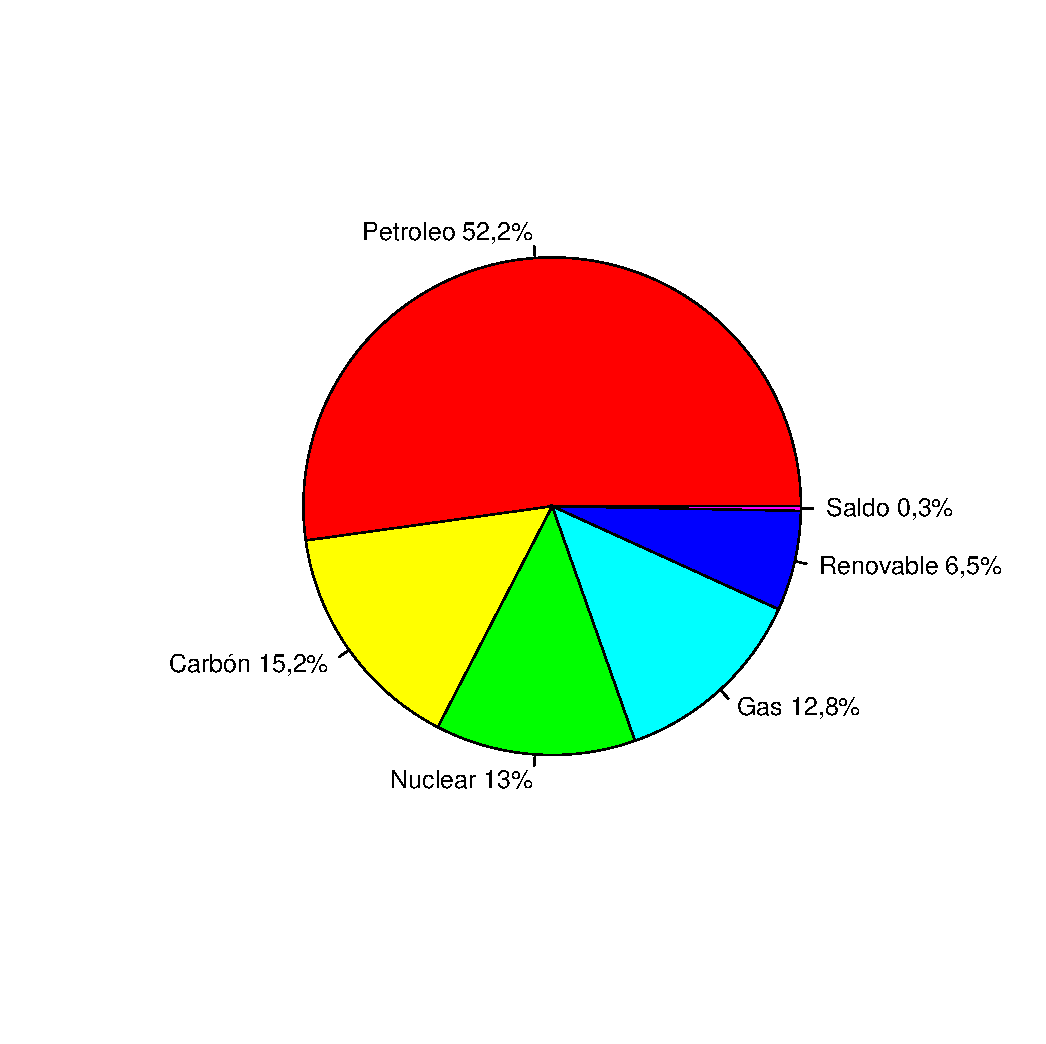
\includegraphics[scale=0.5]{img/energias-des-9}
\]
Realizar un estudio descriptivo de los datos que incluya todos los estadísticos posibles.
}


\newproblem{des-10}{gen}{*}
%ENUNCIADO
{El siguiente diagrama refleja el porcentaje de calificaciones obtenidas en un examen realizado a 80 alumnos:
\[
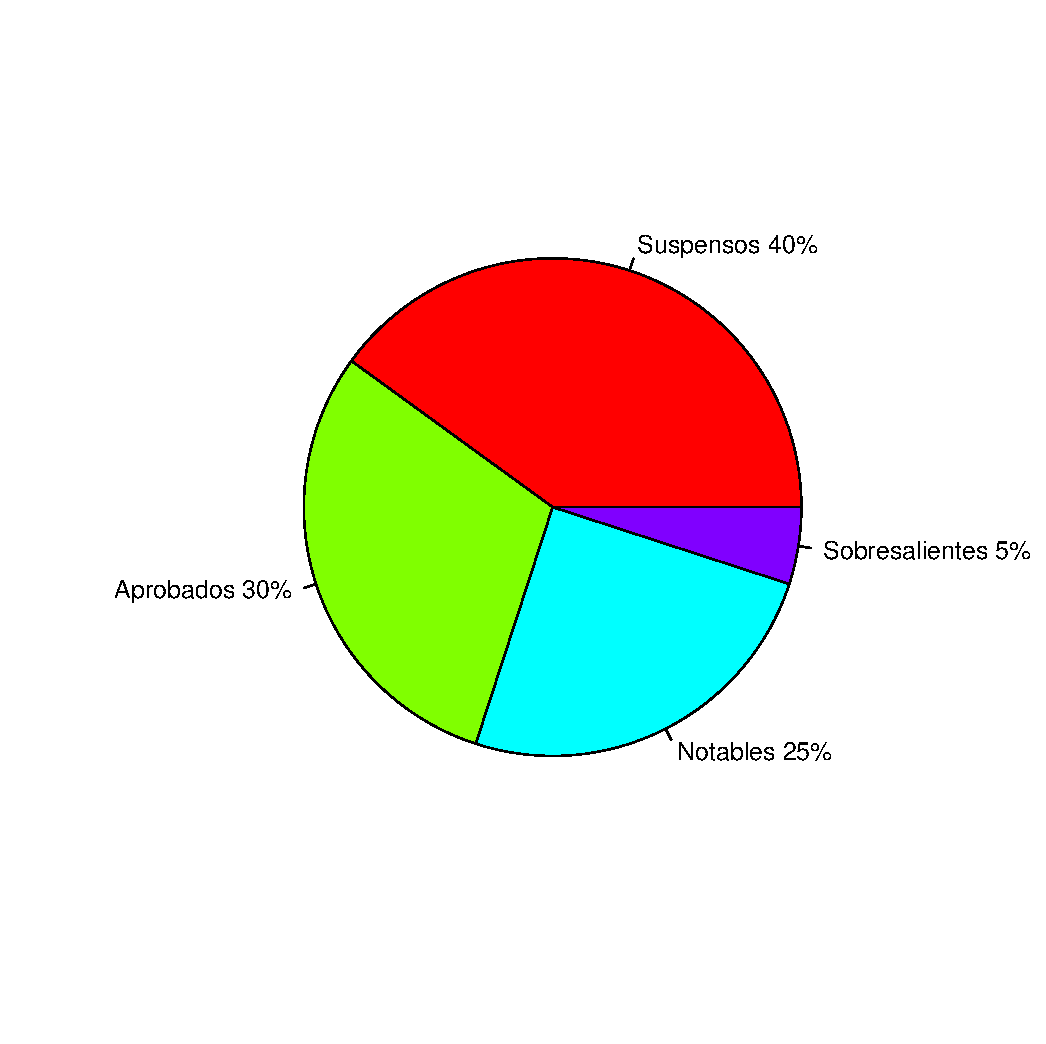
\includegraphics[scale=0.5]{img/sectores-des-10}
\]
Se pide:
\begin{enumerate}
\item Construir la tabla de frecuencias para las calificaciones.
\item Dibujar el polígono de frecuencias acumuladas.
\item Calcular todos los estadísticos de tendencia central que sean posibles.
\item A partir de la variable calificación, construir la variable nota con los siguientes intervalos: Suspenso $[0,5)$, Aprobado $[5,7)$, Notable $[7,9)$ y Sobresaliente $[9,10]$, y calcular la nota media y estudiar su representatividad.
\end{enumerate}
Nota: En los tres primeros apartados se debe trabajar con la variable calificación, mientras que en el último debe utilizarse la variable nota.
}
%SOLUCIÓN
{\begin{enumerate}[start=3]
\item $Me=\mbox{Aprobado}$ y $Mo=\mbox{Suspenso}$.
\item $\bar x = 5.275$ puntos, $s=2.447$ puntos y $cv=0.464$, de manera que la media es moderadamente representativa.  
\end{enumerate}
}
%RESOLUCIÓN
{}


\newproblem{des-11}{gen}{*}
%ENUNCIADO
{Sea la variable estadística agrupada en intervalos cuya distribución de frecuencias viene dada por la siguiente tabla:
\[
\begin{tabular}{|c|c|c|c|c|}
\hline
Intervalos & $n_{i}$ & $f_{i}$ & $N_{i}$ & $F_{i}$ \\ \hline
$\left[ 0,10\right) $ & 10 & 0.25 &  &  \\ \hline
$\left[ 10,20\right) $ &  &  & 22 &  \\ \hline
$\left[ 20,30\right) $ &  & 0.30 &  &  \\ \hline
$\left[ 30,40\right) $ &  &  &  &  \\ \hline
\end{tabular}
\]
\begin{enumerate}
\item  Completar la tabla y hallar la desviación típica.
\item  Calcular la mediana y el rango intercuartílico e interpretarlos.
\end{enumerate}
}
%SOLUCIÓN
{\begin{enumerate}
\item $\bar{x}= 18.5$, $s^2=102.75$ y $s=10.14$. 
\item $Med = 18.33$, $C_1=10$, $C_3 = 26.27$ y $RI= 16.17$ lo que indica, teniendo en cuenta que el rango de toda la distribución es 40, que la dispersión es moderada.
\end{enumerate}
}
%RESOLUCIÓN
{}


\newproblem{des-12}{gen}{}
%ENUNCIADO
{Dada la gráfica correspondiente a un polígono acumulativo de frecuencias relativas de una variable estadística agrupada en intervalos de una muestra de tamaño 20:
\[
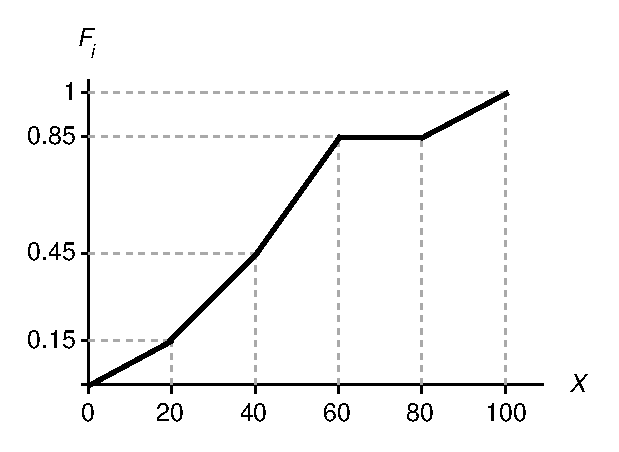
\includegraphics[scale=0.8]{img/poligono-des-12}
\]
se pide:
\begin{enumerate}
\item Construir la tabla de frecuencias.
\item Dibujar el histograma correspondiente.
\item Calcular la mediana y la moda.
\item Calcular la media aritmética y la desviación típica.
\end{enumerate}
}
%SOLUCIÓN
{\begin{enumerate}[start=3]
\item $Med =42.5$ y $Mod= (40,60)$.
\item $\bar = 44$, $s^2 = 564$, $s= 23.75$.
\end{enumerate}
}
%RESOLUCIÓN
{}


\newproblem{des-13}{gen}{*}
%ENUNCIADO
{Dada la siguiente tabla de frecuencias:
\[
\begin{tabular}{|c|c|c|c|c|}
\hline
Intervalos & $n_{i}$ & $f_{i}$ & $N_{i}$ & $F_{i}$ \\ \hline
$\left[ 0,5\right) $ & 2 &  &  &  \\ \hline
$\left[ 5,10\right) $ &  &  & 8 &  \\ \hline
$\left[ 10,15\right) $ &  &  &  & 0.7 \\ \hline
$\left[ 15,20\right) $ & 6 &  &  &  \\ \hline
\end{tabular}
\]
\begin{enumerate}
\item Completar la tabla.
\item Calcular el coeficiente de variación y el rango intercuartílico e interpretar los resultados.
\end{enumerate}
}
%SOLUCIÓN
{$\bar x= 11.5$, $s^2= 24$, $s=4.9$, $cv=0.426$, lo que indica que hay una dispersión moderada. $C_1=7.5$, $C_3=15.83$, $RI=8.33$, lo que indica que la dispersión central también es moderada.
}
%RESOLUCIÓN
{}


\newproblem{des-14}{med}{*}
%ENUNCIADO
{Para obtener información acerca del número de consultas al médico, $X$, que los abonados de una compañía de seguro médico realizan cada mes, trabajando con una muestra de 200 abonados, la distribución de frecuencias fue:
\[
\begin{array}{cc}
\hline
x_i & n_i \\
\hline
0 & 83\\
1 & 51\\
2 & 26\\
3 & 15\\
4 & 9\\
5 & 6\\
6 & 5\\
7 & 3\\
8 & 1\\
9 & 1\\
\hline
\end{array}
\]
Y se pide calcular:
\begin{enumerate}
\item Media, desviación típica y coeficiente de variación del número de visitas al médico. Interpretar el coeficiente de variación.
\item Coeficiente de asimetría de la distribución. Interpretarlo.
\item Percentiles 10 y 90. Interpretarlos.
\end{enumerate}
}
%SOLUCIÓN
{\begin{enumerate}
\item $\bar x=1.41$ consultas, $s^2=3.2919$ consultas$^2$, $s=1.8144$ consultas y $cv=1.29$, lo que indica que hay muchas dispersión y la
media no es muy representativa.
\item $g_1=1.66$ lo cual indica que la distribución es bastante asimétrica hacia la derecha, pero no lo suficiente para considerarla
anormal.
\item $P_{10}=0$ lo que indica que el 10\% de las personas de la muestra que menos consultas realizaron, realizaron 0 consultas, y $P_{90}=4$ lo que indica que el 10\% de las personas de la muestra que más consultas realizaron, realizaron 4 o más consultas.
\end{enumerate}
}
%RESOLUCIÓN
{}


\newproblem{des-15}{med}{*}
%ENUNCIADO
{Los siguientes datos corresponden a 49 mediciones del colesterol HDL (en mg/dl) tomadas en personas de edades y hábitos similares:
\[
\begin{array}{ccccccc}
69.4 & 68.3 & 60.4 & 70.1 & 93.1 & 71.1 & 58.2 \\
73.6 & 70.9 & 71.5 & 57.1 & 58.7 & 56.9 & 74.8 \\
55.6 & 66.6 & 63.7 & 74.5 & 77.3 & 88.0 & 70.3 \\
75.9 & 67.5 & 70.0 & 67.3 & 67.6 & 77.8 & 70.6 \\
64.9 & 68.0 & 85.1 & 72.8 & 61.6 & 69.2 & 69.6 \\
68.1 & 50.1 & 60.2 & 52.0 & 76.4 & 77.2 & 82.4 \\
74.6 & 71.9 & 73.8 & 82.2 & 71.9 & 73.6 & 69.1 \\
\end{array}
\]
\begin{enumerate}
\item Agrupar los datos en 6 clases comenzando en 50 y terminando en $93,2$.
\item Calcular el rango intercuartílico e interpretarlo.
\item Razonar si la media de estos datos es representativa de los mismos.
\end{enumerate}
}
%SOLUCIÓN
{\begin{enumerate}[start=2]
\item $C_1=64.874$ mg/dl, $C_3=75.071$ mg/dl y $RI=10.197$ mg/dl. Esto es bastante menos de la mitad del recorrido de la variable, lo que indica que los datos centrales están bastante concentrados.
\item $\bar x= 69.469$ mg/dl, $s^2=71.952$ (mg/dl)$^2$, $s=8.482$ mg/dl y $cv=0.122$, lo que indica que hay poca dispersión y por tanto la media es muy representativa.
\end{enumerate}
}
%RESOLUCIÓN
{}


\newproblem{des-16}{med}{}
%ENUNCIADO
{Se ha llevado a cabo un estudio sobre el número de radiografías realizadas durante el último año a un grupo de 200 personas, y la información se presenta en la siguiente tabla incompleta:
\[
\begin{array}{|c|c|c|c|}
\hline
\mbox{Radiografías} & \mbox{Personas} & f_i & F_i \\
\hline
0 &    & 0.20 &      \\
1 & 84 &      &      \\
2 &    &      & 0.72 \\
3 &    &      &      \\
4 & 24 &      &      \\
5 &    & 0.02 &      \\  
\hline
\end{array}
\]
\begin{enumerate}
\item Completar tabla.
\item Calcular media, mediana, desviación típica y coeficiente de variación e interpretar los resultados.
\end{enumerate}
}
%SOLUCIÓN
{\begin{enumerate}[start=2]
\item $\bar x= 1.62$ radiografías, $s^2=1.875$ radiografías$^2$, $s=1.37$ radiografías y $cv=0.845$, lo que indica que hay bastante dispersión y la media no es muy representativa.
\end{enumerate}
}
%RESOLUCIÓN
{}


\newproblem{des-17}{far}{*}
%ENUNCIADO
{En un estudio diseñado para investigar la efectividad de un nuevo producto anestésico local, la misma cantidad de producto fue suministrada a 20 pacientes, y se midió el tiempo transcurrido hasta lograr cierto grado de sensibilidad. Los resultados, en minutos, son los siguientes:
\begin{center}
38, 43, 52, 64, 39, 54, 51, 47, 42, 58, 63, 36, 39, 47, 49, 46, 52, 44, 38, 57
\end{center}
\begin{enumerate}
\item Agrupar los datos desde 35 a 65 en 6 clases diferentes.
\item Una vez agrupados, calcular: Media, Desviación Típica y Coeficiente de Asimetría.
\item Teniendo en cuenta la distribución agrupada y suponiendo que todos aquellos datos que se encuentren por arriba del percentil 95 tienen un comportamiento anormal, ¿cuáles de los pacientes se puede considerar que han tenido un tiempo de insensibilidad anormal?
\end{enumerate}
}
%SOLUCIÓN
{\begin{enumerate}[start=2]
\item $\bar x= 47.75$ minutos, $s^2=66.188$ minutos$^2$, $s=8.136$ minutos. $g_1=0.268$ lo que indica que la distribución es ligeramente asimétrica hacia la derecha.
\item $P_{95}=62.5$ minutos. 
\end{enumerate}
}
%RESOLUCIÓN
{}


\newproblem{des-18}{gen}{*}
%ENUNCIADO
{Si a todos los datos de una muestra se les suma una misma cantidad positiva, ¿cómo se ve afectada la representatividad de la media?
¿Y si se multiplican por un mismo número distinto de 0?
Razonar la respuesta.
}
%SOLUCIÓN
{La representatividad de la media aumenta cuando se suma una constante a los datos y se mantiene igual cuando se multiplican por una constante.
}
%RESOLUCIÓN
{Sea $X$ una variable cualquiera y consideremos la variable $Y=X+c$ resultante de sumar una constante $c> 0$ a los valores de $X$. Entonces, aplicando las propiedades de las transformaciones lineales tenemos
\[
cv_{y} = \frac{s_y}{|\bar y|} = \frac{s_x}{|\bar x +c|} < \frac{s_x}{|\bar x|} = cv_{x},
\]
luego al ser menor el coeficiente de variación $Y$ hay menos dispersión relativa y su media es más representativa.

Por otro lado si ahora tomamos $Y=cX$ como la variable resultante de multiplicar los datos de $X$ por una constante $c\neq 0$, tenemos, de nuevo apliando las propiedades de las transformaciones lineales,
\[
cv_{y} = \frac{s_y}{|\bar y|} = \frac{cs_x}{|c\bar x|} = \frac{s_x}{|\bar x|} = cv_{x},
\]
de modo que el coeficiente de variación no se altera y por tanto la representatividad de la media es la misma.
}


\newproblem{des-19}{med}{*}
%ENUNCIADO
{Como parte de un proyecto de investigación, los investigadores obtuvieron los siguientes datos respecto a los niveles de peróxido lípido (en nmol/ml) en el suero de 30 individuos adultos bajo tratamiento de Diabetes Mellitus:
\[
\begin{array}{cccccccccc}
3.09 & 6.06 & 7.34 & 5.32 & 4.29 & 5.36 & 6.01 & 7.84 & 3.87 & 5.23 \\
4.67 & 7.89 & 5.16 & 6.32 & 6.45 & 3.21 & 5.98 & 6.45 & 7.12 & 4.13 \\
5.16 & 3.04 & 4.56 & 5.67 & 5.98 & 6.23 & 7.34 & 5.32 & 4.21 & 7.13 \\
\end{array}
\]
Agrupar los datos en 5 clases de amplitud unidad, comenzando en 3, y sobre la distribución obtenida:
\begin{enumerate}
\item Calcular media, desviación típica y coeficiente de variación de los niveles de peróxido lípido.
Interpretar el coeficiente de variación.
\item Calcular cuartiles de la distribución e interpretarlos.
\item Dibujar el diagrama de caja y bigotes y comprobar si hay o no datos atípicos.
\end{enumerate}
}
%SOLUCIÓN
{\begin{enumerate}
\item $\bar x = 5.667$ nmol/ml, $s^2= 1.668$ (nmol/ml)$^2$, $s= 1.292$ nmol/ml y $cv=0.228$, lo que indica que hay poca dispersión y la media es bastante representativa.
\item $C_1=4.7$ nmol/ml, $C_2=5.667$ nmol/ml y $C_3= 6.75$ nmol/ml.
\item Las vallas son $v_1=1.625$ y $v_2=9.825$. Todos los datos están entre las vallas y no hay datos atípicos. Los bigotes son $b_1=3.04$ nmol/ml y $b_2=7.89$ nmol/ml.
\end{enumerate}
}
%RESOLUCIÓN
{}


\newproblem{des-20}{med}{*}
%ENUNCIADO
{A continuación figura la distribución de edades de una muestra de 65 individuos sujetos a rehabilitación tras un infarto de miocardio:
\begin{center}
\begin{tabular}{|c|c|c|c|c|c|}
\hline
Edad & [40-50) & [50-60) & [60-70) & [70-80) & [80-90)  \\ \hline
$n_i$ & 6 & 12 & 23 & 19 & 5  \\ \hline
\end{tabular}
\end{center}
\begin{enumerate}
\item Sabemos que una distribución normal es simétrica y mesocúrtica.
Por tanto, una primera idea de si los datos muestrales provienen de una distribución normal nos la puede dar ver si estos valores se encuentran en el intervalo [-2, 2].
¿Podríamos suponer según esto que los datos provienen de una distribución normal?
\item Calcular la edad, por encima de la cuál se encuentra el 15\% de los individuos sujetos a rehabilitación tras un infarto de miocardio,
en esta muestra.
\end{enumerate}
}
%SOLUCIÓN
{\begin{enumerate}
\item $\bar x= 65.769$ años, $s^2= 114.823$ años, $s=10.716$ años. $g_1=-0.228$ y $g_2=-0.55$, como tanto el coefiente de asimetría como el de apuntamiento están entre -2 y 2, podemos suponer que los datos provienen de una población normal.
\item $P_{85}=77.5$ años.  
\end{enumerate}
}
%RESOLUCIÓN
{}


\newproblem{des-21}{med}{*}
%ENUNCIADO
{Para obtener información acerca del porcentaje de albúmina en el suero proteico de personas adultas, se analizaron muestras de 32 personas, con los siguientes resultados:
\[
\begin{array}{cccccccc}
70.2 & 63.5 & 65.8 & 67.9 & 60.1 & 69.7 & 64.2 & 65.3 \\
62.8 & 68.4 & 65.2 & 66.3 & 70.7 & 71.8 & 68.7 & 71.9 \\
64.4 & 62.4 & 60.4 & 67.0 & 62.9 & 65.9 & 67.5 & 66.6 \\
67.8 & 70.5 & 63.1 & 65.3 & 69.5 & 71.4 & 61.0 & 64.3 \\
\end{array}
\]
\begin{enumerate}
\item Agrupar la distribución de porcentajes de albúmina en 6 clases de igual amplitud, desde 60 hasta 72.
\item En la distribución agrupada calcular media, desviación típica, y cuartiles.
\item ¿Es representativa la media de la muestra de porcentajes de albúmina?
\item Dibujar el diagrama de caja y bigotes de la distribución y determinar si hay o no algún dato atípico.
\end{enumerate}
}
%SOLUCIÓN
{\begin{enumerate}[start=2]
\item $\bar x=66.3125\%$, $s^2=9.9023\%^2$, $s=3.1468\%$. $C_1=64\%$, $C_2=66\%$, $C_3=69\%$.
\item $cv=0.05$ lo que indica que hay muy poca dispersión y la media es muy representativa.
\end{enumerate}
}
%RESOLUCIÓN
{}


\newproblem*{des-22}{amb}{}
%ENUNCIADO
%CAMBIAR DATOS PARA QUE SALGA MÁS ASIMÉTRICA
{Para determinar la validez de un terreno para un determinado cultivo, se realizó un muestreo sistemático del terreno obteniendo 18 valoraciones del PH del suelo-agua (en relación 1:2.5).
Los valores obtenidos fueron:
\[
\begin{array}{ccccccccc}
5.82 & 6.23 & 6.17 & 7.11 & 6.44 & 6.08 & 6.03 & 5.91 & 6.83 \\
6.55 & 6.24 & 6.12 & 6.32 & 5.86 & 6.64 & 6.73 & 7.24 & 6.02
\end{array}
\]
Se pide:
\begin{enumerate}
\item Calcular el coeficiente de asimetría e interpretarlo.
\item Aplicar una transformación a la variable para obtener otra variable con una simetría más normal.
\end{enumerate}
}


\newproblem{des-23}{far}{}
%ENUNCIADO
{Para determinar la eficacia de un nuevo método para la medición del hematocrito en sangre, se repitió la medida 8 veces sobre una misma muestra de sangre, obteniéndose los siguientes resultados (en porcentaje de hematocrito sobre volumen de plasma sanguíneo):
\[
\begin{array}{cccccccc}
42.2 & 42.1 & 41.9 & 41.8 & 42 & 42.1 & 41.9 & 42.
\end{array}
\]
¿Se puede afirmar que se trata de un buen método de medición?
}
%SOLUCIÓN
{$\bar x= 42\%$, $s^2=0.015\%^2$, $s=0.1225\%$ y $cv=0.003$ lo que indica que la variabilidad entre las mediciones es ínfima y por tanto se trata de un buen método de medición.
}
%RESOLUCIÓN
{Para ver si se trata de un buen método de medición, tenemos que comprobar que entre las sucesivas mediciones no haya grandes diferencias. Se trata, por tanto, de medir la variabilidad de la muestra y para ello calculamos el coeficiente de variación:
\begin{align*}
\bar x & = \frac{\sum x_i}{n} = \frac{42.2+\cdots+42}{8} = \frac{336}{8}= 42\%,\\
s^2 & = \frac{\sum x_i^2}{n}-\bar x^2 = \frac{42.2^2+\cdots+42^2}{8}-42^2 = \frac{14112.12}{8}-42^2= 0.015\%^2,\\
s &= \sqrt{0.015} = 0.1225\%,\\
cv &= \frac{s}{|\bar x|} = \frac{0.1225}{42} = 0.003.
\end{align*}
Como el coeficiente de variación es muy pequeño, podemos concluir que la variabilidad entre las mediciones es ínfima y por tanto se trata de un buen método de medición.
}


\newproblem{des-24}{fis}{}
%ENUNCIADO
{En cuestionario sobre la dependencia de las personas mayores de 75 años se preguntaba sobre la necesidad de ayuda en el desarrollo normal de su vida. Las posibles respuestas eran:
\begin{enumerate}
\item Ninguna ayuda.
\item Ayuda al subir las escaleras.
\item Ayuda al subir las escaleras y al incorporarse de una posición sentada o tumbada.
\item Ayuda al subir las escaleras, al incorporarse, y al vestirse.
\item Ayuda para prácticamente todo.
\end{enumerate}
El cuestionario lo respondieron 20 personas, y los resultado obtenidos fueron
\begin{center}
b -- d -- a -- b -- c -- c -- b -- c -- d -- e -- a -- b -- c -- e -- a -- b -- c -- d -- b -- b
\end{center}
Se pide:
\begin{enumerate}
\item Representar gráficamente la distribución de frecuencias.
\item Calcular las medidas de tendencia central.
\item Calcular los cuartiles y el decil 8.
\item ¿Qué se puede decir sobre la dispersión?
\end{enumerate}
}
%SOLUCIÓN
{\begin{enumerate}[start=2]
\item $Me$ ente b y c y $Mo=b$. 
\item $C_1=$b, $C_2$ entre b y c, $C_3=$ entre c y d, $D_8=d$.
\item Suponiendo que hay la misma distancia entre categorías y asignando rangos a cada valor ($a=1,b=2,c=3,d=4,e=5$), tenemos $\bar x=2.7$, $s^2=1.41$, $s=1.187$ y $cv=0.44$, lo que indica una dispersión moderada. 
\end{enumerate}
}
%RESOLUCIÓN
{}


\newproblem{des-25}{amb}{*}
%ENUNCIADO
{Como parte de un proyecto de investigación, los investigadores obtuvieron los siguientes datos respecto a los niveles (en partes por millón) de cierto contaminante químico en 30 suelos diferentes de la Comunidad de Madrid:
\begin{center}
\[
\begin{array}{cccccccccc}
3.09 & 6.06 & 7.34 & 5.32 & 4.29 & 5.36 & 6.01 & 7,84 & 3.87 & 5.23 \\
4.67 & 7.89 & 5.16 & 6.32 & 6.45 & 3.21 & 5.98 & 6.45 & 7.12 & 4.13 \\
5.16 & 3.04 & 4.56 & 5.67 & 5.98 & 6.23 & 7.34 & 5.32 & 4.21 & 7.13 \\
\end{array}
\]
\end{center}
Agrupar los datos en 5 clases de amplitud unidad, comenzando en 3, y sobre la distribución obtenida:
\begin{enumerate}
\item Calcular media, desviación típica y coeficiente de variación de los niveles de contaminante.
Interpretar el coeficiente de variación.
\item Calcular cuartiles de la distribución e interpretarlos.
\item Dibujar el diagrama de caja y bigotes y comprobar si hay o no datos atípicos.
\end{enumerate}
}
%SOLUCIÓN
{\begin{enumerate}
\item $\bar x = 5.667$ ppm, $s^2= 1.668$ ppm$^2$, $s= 1.292$ ppm y $cv=0.228$, lo que indica que hay poca dispersión y la media es bastante representativa.
\item $C_1=4.7$ ppm, $C_2=5.667$ ppm y $C_3= 6.75$ ppm.
\item Las vallas son $v_1=1.625$ y $v_2=9.825$. Todos los datos están entre las vallas y no hay datos atípicos. Los bigotes son $b_1=3.04$ ppm y $b_2=7.89$ ppm.
\end{enumerate}
}
%RESOLUCIÓN
{}


\newproblem{des-26}{fis}{*}
%ENUNCIADO
{Se desea realizar un estudio sobre los días necesarios para tratar una determinada lesión deportiva.
Se utilizaron para ello dos tratamientos diferentes, y se observaron 50 pacientes con cada uno de los tratamientos, obteniendo los siguientes resultados:
\begin{center}
\begin{tabular}{|c|c|c|}
\hline
Nº Sesiones & Tratamiento A & Tratamiento B \\
\hline
20-40 & 5 & 8  \\
\hline
40-60 & 20 & 15  \\
\hline
60-80 & 18 & 20  \\
\hline
80-100 & 7 & 7  \\
\hline
\end{tabular}
\end{center}
\begin{enumerate}
\item Calcular el número de sesiones por debajo del cual está el 86\% de los pacientes, en cada tratamiento.
\item ¿En cuál de los dos tratamientos es más representativa la media del número de sesiones necesarias?
Justificar numéricamente la respuesta.
\item ¿Qué distribución presenta mayor asimetría?
Justificar numéricamente la respuesta.
\end{enumerate}
}
%SOLUCIÓN
{\begin{enumerate}
\item Tratamiento $A$: $P_{86} = 80$ sesiones. Tratamiento $B$: $P_{86}=80$ sesiones.
\item $\bar x_A=60.8$ sesiones, $s^2_A=291.36$ sesiones$^2$, $s_A=17.0693$ sesiones y $cv_A = 0.28$.\\
$\bar x_B=60.4$ sesiones, $s^2_B= 339.84$ sesiones$^2$, $s_B=18.4348$ sesiones y $cv_B = 0.31$.\\
Así pues, como $cv_A<cv_B$ la media es un poco más representativa para el tratamiento $A$. 
\item $g_{1_A} = 0.068$ y $g_{1_B} = -0.14$ lo que indica que la distribución para el tratamiento $A$ es ligeramente asimétrica hacia la derecha y la del tratamiento $B$ ligeramente asimétrica hacia la izquierda, aunque ambas son casi simétricas. 
\end{enumerate}
}
%RESOLUCIÓN
{}


\newproblem{des-27}{gen}{*}
%ENUNCIADO
{El número de muertos en  accidentes de carretera durante el 2005 en España fue el siguiente
\begin{center}
\begin{tabular}{|l|cccccccccccc|}
\hline
Mes & Ene & Feb & Mar & Abr & May & Jun & Jul & Ago & Sep & Oct & Nov & Dic\\
\hline
Muertos & 272 & 269 & 293 & 274 & 308 & 314 & 374 & 354 & 310 & 318 & 269 & 297\\
\hline
\end{tabular}
\end{center}
Se pide:
\begin{enumerate}
\item Calcular el coeficiente de variación del número mensual de muertos e interpretarlo.
\item Calcular la mediana del número mensual de muertos.
\end{enumerate}
}
%SOLUCIÓN
{\begin{enumerate}
\item $\bar x=304.333$ muertos, $s^2=1024.425$ muertos$^2$, $s=32.007$ muertos y $cv =0.105$, lo que indica que hay poca variabilidad en los datos y la media es muy representativa.
\item $Me=302.5$ muertos.
\end{enumerate}
}
%RESOLUCIÓN
{\begin{enumerate}
\item Para calcular el coeficiente de variación necesitamos tanto la media como la desviación típica de la variable. Si llamamos $X$ al número mensual de muertos, teniendo en cuenta que los valores se repiten una única vez, y trabajando con ellos sin agrupar, ya que sólo tenemos 12 valores diferentes correspondientes a los 12 meses
del año, podemos completar fácilmente la tabla necesaria para el cálculo:
\[
\begin{array}{|c|c|}
\hline
x_i & x_i^2 \\
\hline
272 & 73984 \\
269 & 72361 \\
293 & 85849 \\
274 & 75076 \\
308 & 94864 \\
314 & 98596 \\
374 & 139876 \\
354 & 125316 \\
310 & 96100 \\
318 & 101124 \\
269 & 72361 \\
297 & 88209 \\
\sum x_i=2652 & \sumx_i^2=1123716 \\
\hline
\end{array}
\]

Con ello:
\begin{align*}
\bar x &= \frac{{\sum {x_i} }} {12} = \frac{{3651}} {{12}} = 304.333\\
s^2  &= \frac{{\sum {x_i ^2} }} {12} - \bar x^2 = \frac{{1123716}}
{{12}} - 304.333^2  = 1024.425 \Rightarrow s = + \sqrt {1024.425} =
32.007
\end{align*}

Y el coeficiente de variación vale:
\[
Cv = \frac{s}{{\left| {\bar x} \right|}} =
\frac{{32.007}}{{304.333}} = 0.105=10.5\%
\]
Por lo tanto, la dispersión relativa de la muestra es bastante pequeña ($10.5\%$) y podemos afirmar que la media de la distribución es bastante representativa.

\item Ordenando los datos de menor a mayor obtenemos la siguiente secuencia:
\[
269,269,272,274,293,297,308,310,314,318,354,374
\]

Y para calcular la mediana, una vez ordenados los 12 datos de mayor a menor, nos debemos fijar en los valores de la variable que ocupan las dos posiciones centrales, sexta y séptima, ya que tenemos un número par de datos. En la sexta posición encontramos 297 muertos, y en la séptima 308. Por lo tanto:
\[
Me = \frac{{297 + 308}}{2} = 302.5
\]
\end{enumerate}
}


\newproblem*{des-28}{med}{*}
%ENUNCIADO
{Un médico de familia analiza el número de recetas que ha expedido entre sus abonados en los dos últimos meses, obteniendo la siguiente distribución:
\begin{center}
\begin{tabular}{|l|ccccccccc|}
\hline
Recetas & 0 & 1 & 2 & 3 & 4 & 6 & 7 & 9 & 12\\
\hline
Abonados & 401 & 203 & 95 & 150 & 166 & 40 & 10 & 12 & 3\\
\hline
\end{tabular}
\end{center}

\begin{enumerate}
\item Calcular la media, desviación tí­pica y coeficiente de variación del número de recetas e interpretar este último.
\item Si un número medio de recetas superior a 2 puede suponer un fraude, ¿existen pruebas significativas para afirmar que no hay fraude? Justificar la respuesta.
\item Teniendo en cuenta la definición dada más abajo, calcular le Media Recortada 10\% ($MR_{0.1}$) del número de recetas.
¿Cuándo crees que será conveniente la utilización de la media recortada en lugar de la media aritmética?\\
\textbf{Definición}: La \emph{media recortada} $p$\% es la media aritmética de la muestra que queda al quitar el $p$\%
de valores menores y el $p$\% de valores mayores de la muestra original.
\end{enumerate}
}


\newproblem{des-29}{far}{*}
%ENUNCIADO
{El siguiente histograma refleja la distribución del índice de masa corporal en una muestra de hombres y mujeres.
\begin{center}
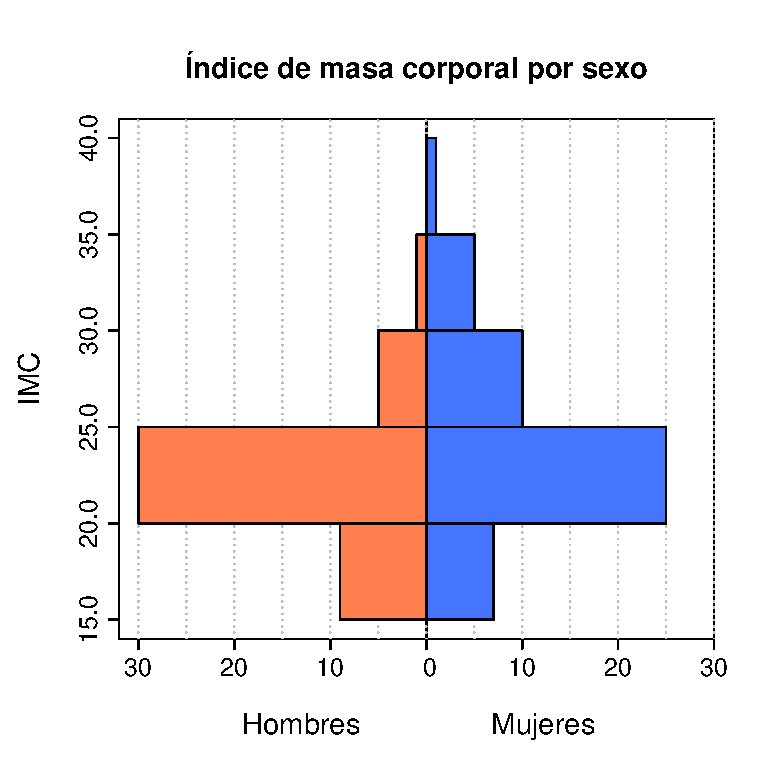
\includegraphics[scale=0.7]{img/histograma-des-29}
\end{center}
Se pide:
\begin{enumerate}
\item Construir la tabla de frecuencias para hombres y mujeres por separado.
\item Dibujar el diagrama de sectores para el sexo.
\item ¿En qué grupo es más representativa la media? Justificar la respuesta.
\item ¿Cómo calcularías la media de toda la muestra a partir de las medias de hombres y mujeres? ¿Cuánto vale?
\item Calcular el rango intercuartílico del índice de masa corporal en los hombres.
\end{enumerate}
}
%SOLUCIÓN
{\begin{enumerate}[start=3]
\item $\bar{m} =24.17$ Kg/m$^2$, $s_{m}^2=21.1806$ (Kg/m$^2$)$^2$, $s_m=4.6$ Kg/m$^2$ y $cv_m = 0.19$.\\
$\bar{h} =22.28$ Kg/m$^2$, $s_{m}^2=9.9506$ (Kg/m$^2$)$^2$, $s_m=3.15$ Kg/m$^2$ y $cv_h = 0.14$, luego es más representativa la media en los
hombres.
\item $\bar{x}=23.25$ Kg/m$^2$.
\item $RI=3.75$ Kg/m$^2$.
\end{enumerate}
}
%RESOLUCIÓN
{Lamemos $H$ a la variable que mide el índice de masa corporal para los hombres y $M$ para las mujeres.
\begin{enumerate}
\item A partir del histograma de frecuencias absolutas de las mujeres podemos obtener fácilmente las frecuencias absolutas de los intervalos mirando la altura de las barras, y a partir de las frecuencias absolutas podemos calcular el resto de frecuencias.
La tabla de frecuencias para las mujeres es:
\[
\begin{array}{|c|r|r|r|r|}
\hline
   M   & n_i &  f_i & N_i &  F_i \\
\hline
 15-20 &   7 & 0.15 &   7 & 0.15 \\
 20-25 &  25 & 0.52 &  32 & 0.67 \\
 25-30 &  10 & 0.21 &  42 & 0.88 \\
 30-35 &   5 & 0.10 &  47 & 0.98 \\
 35-40 &   1 & 0.02 &  48 & 1.00 \\
\hline
\mbox{Suma} & 48 & 1.00 & & \\
\hline
\end{array}
\]
Del mismo modo, a partir del histograma de frecuencias absolutas de los hombres obtenemos la tabla de frecuencias para hombres:
\[
\begin{array}{|c|r|r|r|r|}
\hline
   H   & n_i &  f_i & N_i &  F_i \\
\hline
 15-20 &   9 & 0.20 &   9 & 0.20 \\
 20-25 &  30 & 0.67 &  39 & 0.87 \\
 25-30 &   5 & 0.11 &  44 & 0.98 \\
 30-35 &   1 & 0.02 &  45 & 1.00 \\
\hline
\mbox{Suma} & 45 & 1.00 & & \\
\hline
\end{array}
\]

\item La variable Sexo sólo tiene dos categorías que son Hombre y Mujer, de modo que el diagrama de sectores asociado sólo tendrá dos sectores. La tabla de frecuencias de la variable sexo es:
\[
\begin{array}{|c|r|r|}
\hline
  \textrm{Sexo}  & n_i &   f_i \\
\hline
 \textrm{Mujer}  &  48 & 0.516 \\
\hline
 \textrm{Hombre} &  45 & 0.484 \\
\hline
  \textrm{Suma}  &  93 & 1.000 \\
\hline
\end{array}
\]
Así pues, para calcular el ángulo correspondiente a cada sector basta con multiplicar $360^{\circ}$ (el ángulo de la circunferencia completa) por la frecuencia relativa de cada categoría:
\[
\alpha_m=360^{\circ}0.516=186^{\circ}\qquad \alpha_h=360^{\circ}0.484=174^{\circ}.
\]
Y el diagrama de sectores asociados es:
\begin{center}
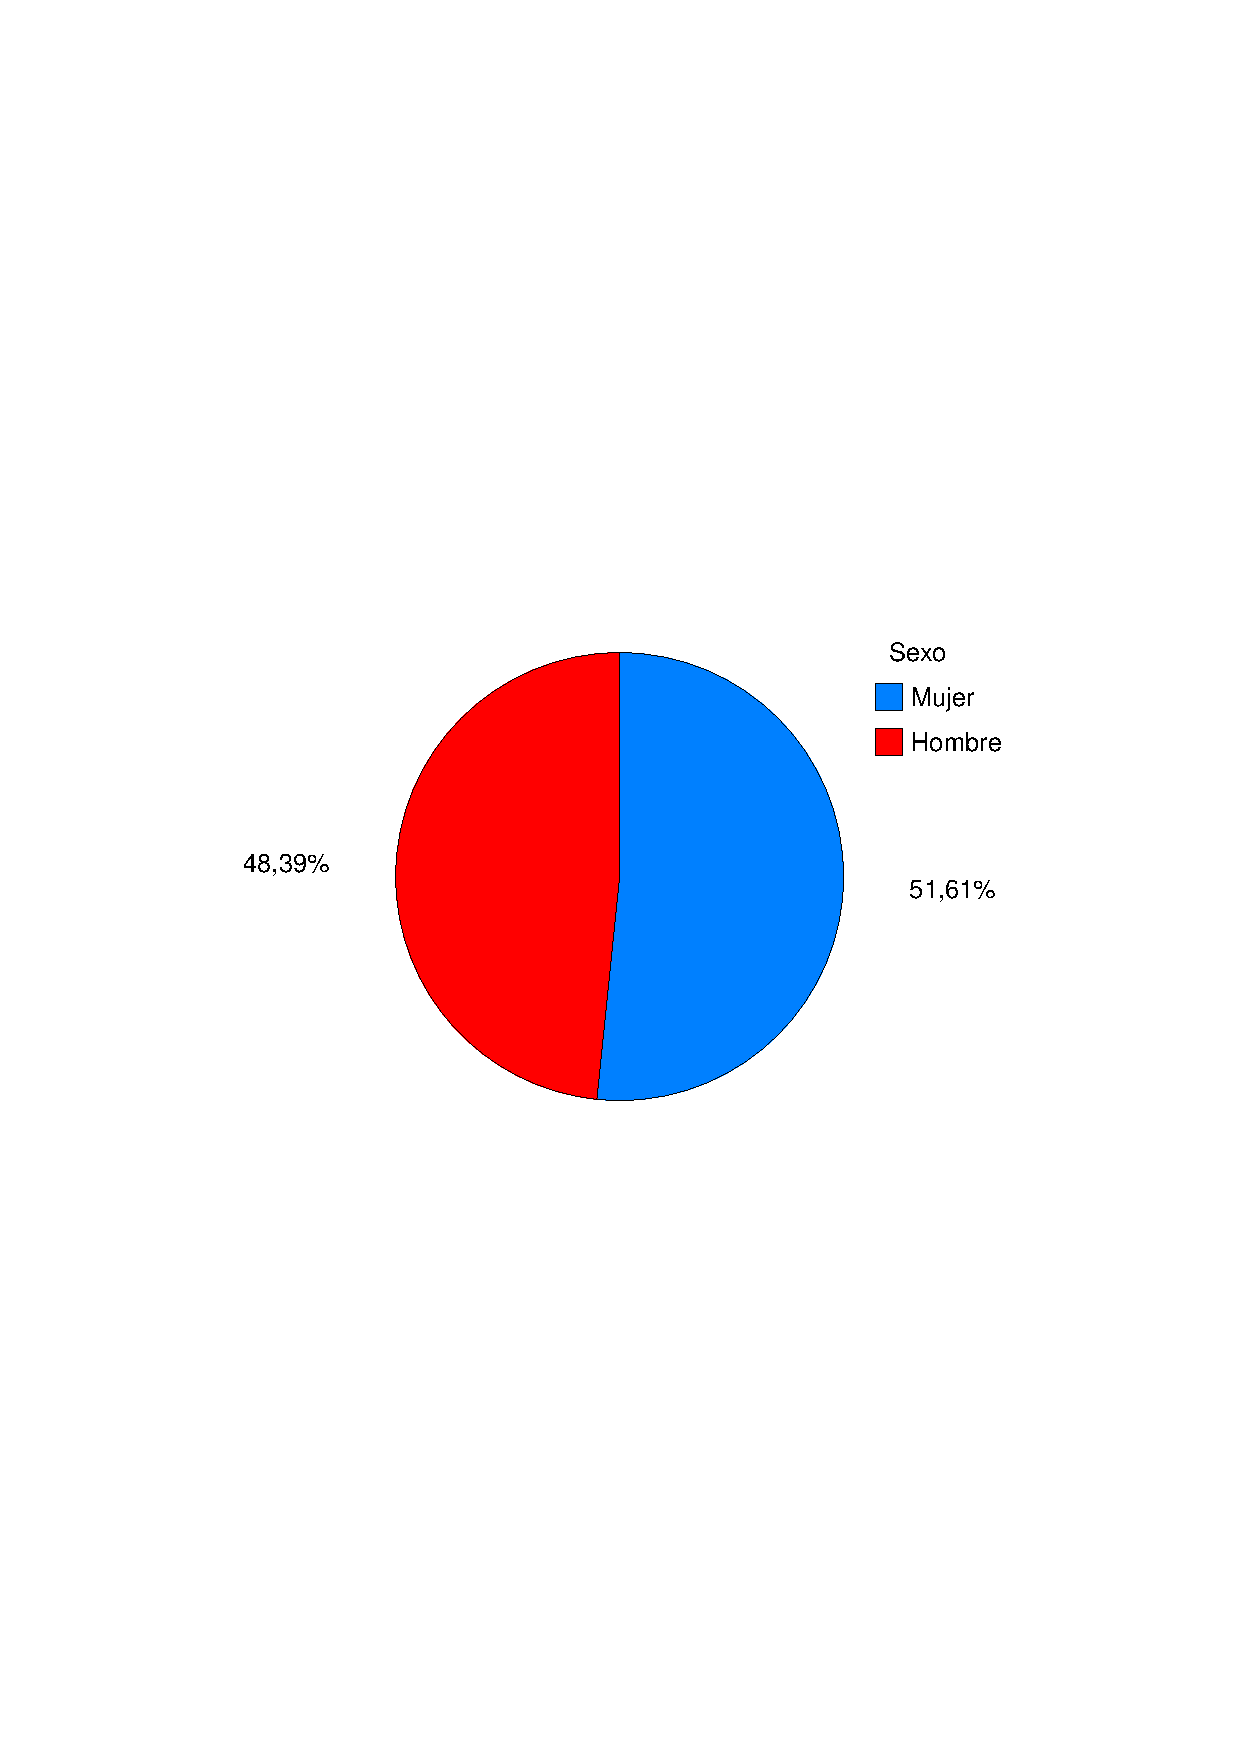
\includegraphics[scale=0.6]{img/sectores-des-29}
\end{center}

\item La media será más representativa en el grupo que tenga menos dispersión, y para comparar la dispersión de ambos grupos necesitamos el coeficiente de variación.
Calculamos para ello los estadísticos necesarios a partir de las tablas de frecuencias. Para las mujeres tenemos:
\[
\begin{array}{|c|r|r|r|r|}
\hline
   M   & m_i & n_i & m_in_i & m_i^2n_i \\
\hline
 15-20 & 17.5 &  7 & 122.5 & 2143.75 \\
 20-25 & 22.5 & 25 & 562.5 & 12656.25\\
 25-30 & 27.5 & 10 & 275.0 & 7562.50 \\
 30-35 & 32.5 &  5 & 162.5 & 5281.25 \\
 35-40 & 37.5 &  1 &  37.5 & 1406.25 \\
\hline
\mbox{Suma} & & 48 & 1160.0& 29050.00 \\
\hline
\end{array}
\]

\begin{align*}
\bar{m} & = \frac{\sum m_{i}}{n_m}=\frac{1160}{48}=24.17,  \\
s_{m}^2 &= \frac{\sum m_{i}^2}{n_m}-\bar{m}^2 = \frac{29050}{48}-24.17^2=21.1806,  \\
s_m &= \sqrt{21.1806} = 4.6,\\
cv_m &= \frac{s_m}{|\bar{m}|}=\frac{4.6}{24.17} = 0.19.
\end{align*}

Y para los hombres:
\[
\begin{array}{|c|r|r|r|r|}
\hline
   H   & h_i &  n_i & h_in_i &  h_i^2n_i \\
\hline
 15-20 &  17.5 &  9 & 157.5 &  2756.25 \\
 20-25 &  22.5 & 30 & 675.0 & 15187.50 \\
 25-30 &  27.5 &  5 & 137.5 &  3781.25 \\
 30-35 &  32.5 &  1 &  32.5 &  1056.25 \\
\hline
\mbox{Suma} & & 45 & 1002.5 & 22781.25 \\
\hline
\end{array}
\]

\begin{align*}
\bar{h} & = \frac{\sum h_{i}}{n_h}=\frac{1002.5}{45}=22.28,  \\
s_{h}^2 & = \frac{\sum h_{i}^2}{n_h}-\bar{h}^2 =
\frac{22781.25}{45}-22.28^2=9.9506,  \\
s_h &= \sqrt{9.9506} = 3.15,\\
cv_h &= \frac{s_h}{|\bar{h}|}=\frac{3.15}{22.28} = 0.14.
\end{align*}

Así pues, ambas muestras tienen un coeficiente de variación bajo y por tanto las medias son muy representativas, pero lo es un poco más la de los hombres ya que tienen una poca menos dispersión.

\item Para calcular la media de toda la muestra podemos hacer una media ponderada de las medias de las mujeres y l
os hombres donde los pesos son los tamaños muestrales de cada grupo.
\[
\bar{x}=\frac{p_m\bar{m}+p_h\bar{h}}{p_m+p_h}=\frac{45\cdot 22.28+48\cdot 24.17}{45+48}=23.25.
\]

\item El rango intercuartílico es la diferencia entre el tercer y el primer cuartil, así que procedemos a calcular ambos cuartiles.
La frecuencia acumulada correspondiente al primer cuartil es $n_h/4=11.25$, lo cual nos indica, mirando la columna de frecuencia acumuladas de los hombres, que dicho cuartil está en el intervalo $20-25$.
Interpolando en dicho intervalo tenemos:
\[C_1=20+\frac{11.25-9}{30}5 = 20.375.\]
Del mismo modo, la frecuencia acumulada correspondiente al tercer cuartil es $3n_h/4=33.75$, lo que indica que este cuartil también está en el intervalo $20-25$.
Interpolando en dicho intervalo tenemos:
\[C_3=20+\frac{33.75-9}{30}5 = 24.125.\]
Así pues, el rango intercuartílico es $RI=C_3-C_1=24.125-20.375=3.75$.
\end{enumerate}
}


\newproblem*{des-30}{med}{*}
%ENUNCIADO
{Se ha medido el tiempo necesario, en días, para curar un tipo concreto de infección (tiempo transcurrido desde el comienzo del tratamiento hasta el alta) en dos grupos de pacientes a los que se han aplicado antibióticos diferentes.
En un grupo de 80 pacientes tratados con el antibiótico A, los resultados obtenidos fueron:
\[
\begin{array}{|c|c|}
\hline
\mbox{Tiempo (días)} & n_i \\
\hline
{[0,30)} & 50 \\
{[30,60)} & 20 \\
{[60,90)} & 10 \\
\hline
\end{array}
\]

Mientras que en un grupo de 100 pacientes tratados con el antibiótico B se obtuvo:
\[
\begin{array}{|c|c|}
\hline
\mbox{Tiempo (días)} & n_i \\
\hline
{[0,30)} & 40 \\
{[30,60)} & 50 \\
{[60,90)} & 10 \\
\hline
\end{array}
\]

\begin{enumerate}
\item Calcular la media y la desviación típica del número de días hasta el alta, para cada uno de los antibióticos.
\item ¿En qué antibiótico es más representativa la media?. Justificar la respuesta numéricamente.
\item ¿Cuánto vale el percentil 90 del tiempo de curación para los pacientes tratados con B?
\item ¿Qué tiempo de recuperación ha sido relativamente más alto, uno de 40 días de un paciente tratado con A, o uno de 45 días de otro tratado con B? Justificar la respuesta numéricamente.
\end{enumerate}
}


\newproblem{des-31}{med}{*}
%ENUNCIADO
{Para  estudiar la eficacia de un nuevo fármaco en el tratamiento de la hipertensión arterial, se tomaron los valores
de la tensión arterial diastólica (TAD) en 8 pacientes antes del tratamiento ($X$) y después de un mes de tratamiento
($Y$), obteniéndose los siguientes resultados:
\begin{center}
\begin{tabular}{|c|r|r|r|r|r|r|r|r|}
\hline
$X$ & 100 & 104 & 96 & 98 & 105 & 106 & 110 & 100 \\
\hline
$Y$ & 92 & 97 & 94 & 100 & 94 & 92 & 95 & 104 \\
\hline
\end{tabular}
\end{center}

\begin{enumerate}
\item ¿En qué variable es más representativa la media?
\item Hallar el coeficiente de asimetría de la variable $Y$ e interpretarlo.
\end{enumerate}
}
%SOLUCIÓN
{\begin{enumerate}
\item $\bar x=102.375$, $s_x^2=18.9844$, $s_x=4.3571$ y $cv_x =0.0426$.\\
$\bar y=96$, $s_y^2=15.25$, $s_y=3.9051$ y $cv_y = 0.0407$.\\
Como ambos coeficientes de variación son casi iguales podemos concluir que ambas medias son igual de representativas.
\item $g_1=0.9068$ lo que indica que es asimétrica hacia la derecha.
\end{enumerate}
}
%RESOLUCIÓN
{\begin{enumerate}
\item Para ver en qué muestra es más representativa la media tenemos que comparar las dispersiones de ambas muestras mediante el coeficiente de variación. Para ello, procedemos al cálculo de los estadísticos necesarios:
\begin{align*}
\bar{x} & = \frac{\sum x_{i}}{n}=\frac{100+\cdots+100}{8}=\frac{819}{8}=102.375,  \\
s_{x}^2 & = \frac{\sum x_{i}^2}{n}-\bar{x}^2 =
\frac{100^2+\cdots+100^2}{8}-102.375^2=\frac{83997}{8}-10480,6406=18.9844,  \\
s_{x} & = \sqrt{18.9844}=4.3571,  \\
cv_x &= \frac{s_x}{|\bar{x}|}= \frac{4.3571}{102.375}=0.0426,\\
\bar{y} & = \frac{\sum y_{j}}{n}=\frac{92+\cdots+104}{8}=
\frac{768}{8}=96,  \\
s_{y}^2 & = \frac{\sum y_{j}^2}{n}-\bar{y}^2 =
\frac{92^2+\cdots+104^2}{8}-96^2=\frac{73850}{8}-9216=15.25,  \\
s_{y} & = \sqrt{15.25}=3.9051,  \\
cv_y &= \frac{s_y}{|\bar{y}|}= \frac{3.9051}{96}=0.0407,\\
\end{align*}
Ambos coeficientes de variación son muy pequeños, lo cual indica que hay muy poca dispersión en las muestras y las medias son muy representativas, aunque un poco más la de $Y$ por tener un coeficiente de variación más pequeño.

\item El coeficiente de asimetría de $Y$ es 
\[g_1=\frac{\sum(y_j-\bar{y})^3/n}{s_y^3}=
\frac{\left((92-96)^3+\cdots +(104-96)^3\right)/8}{3.9051^3}=\frac{432/8}{59,552}=0.9068,\]
lo que indica que la distribución es asimétrica a la derecha aunque no los suficiente como para rechazar la hipótesis de que los datos provienen de una población normal.
\end{enumerate}
}


\newproblem{des-32}{amb}{*}
%ENUNCIADO
{Una piscifactoría realiza un estudio para determinar si una especie de pez está en peligro extinción en los ríos de una región.
Para ello se midió el número de peces en 10 sitios diferentes obteniendo los siguientes resultados en unidades
por hectómetro cúbico:
\begin{center}
  36 -- 11 -- 7 -- 18 -- 35 -- 27 -- 21 -- 15 -- 25 -- 12
\end{center}
Se pide:
\begin{enumerate}
\item Calcular las medidas de tendencia central.
\item Calcular el coeficiente de apuntamiento e interpretarlo.
\end{enumerate}
}
%SOLUCIÓN
{\begin{enumerate}
\item $\bar{x} = 20.7$ peces, $Me=19.5$ peces, no hay moda porque todos los valores tienen frecuencia 1. 
\item $g_2= -1.13$ lo que indica que es una distribución bastante platicúrtica. 
\end{enumerate}
}
%RESOLUCIÓN
{Llamemos $X$ al número de peces por hectómetro cúbico.
\begin{enumerate}
\item Las medidas de tendencia central son la media aritmética, la mediana y la moda. Calculamos primero la media:
\[
\bar{x} = \frac{\sum x_{i}}{n}=\frac{36+\cdots+12}{10}=\frac{207}{10}=20.7 \mbox{ peces},
\]

Para calcular la mediana ordenamos los valores de la muestra:
\begin{center}
  7 -- 11 -- 12 -- 15 -- 18 -- 21 -- 25 -- 27 -- 35 -- 36
\end{center}
Como el tamaño de la muestra es par, habrá dos individuos que ocupen las posiciones centrales de la muestra, y estos serán los que ocupen las posiciones $n/2=10/2=5$ y $n/2+1=6$, es decir, los valores 18 y 21. Así pues la mediana es
\[
Me=\frac{18+21}{2}=19.5 \mbox{ peces}.
\]

Por último, no podemos decir que haya moda porque todos los valores tienen frecuencia 1.

\item La fórmula del coeficiente de apuntamiento es 
\[
g_2=\frac{\sum (x_i-\bar{x})^4}{ns^4}-3,
\]
así que necesitamos calcular previamente la desviación típica:
\begin{align*}
s^2 & = \frac{\sum x_{i}^2}{n}-\bar{x}^2 =
\frac{36^2+\cdots+12^2}{10}-20.7^2=\frac{5179}{10}-428,49=89.41,\\
s &=\sqrt{89.41}=9.4557.
\end{align*}
Así pues, tenemos
\[
g_2=\frac{(36-20.7)^4+\cdots + (12-20.7)^4}{10\cdot 9.4557^4}-3=\frac{149449.657}{79941,9504}-3=-1.13,
\]
lo que indica que la distribución es bastante platicúrtica, es decir, con menos apuntamiento que una distribución normal.
\end{enumerate}
}


\newproblem{des-33}{amb}{*}
%ENUNCIADO
{Las temperaturas (en ºC) observadas en Barcelona y La Coruña en 12 días elegidos aleatoriamente el último año fueron:
\begin{center}
\begin{tabular}{|l|cccccccccccc|}
\hline
Barcelona & 13 & 14 & 16 & 18 & 21 & 25 & 28 & 28 & 25 & 21 & 17 & 13\\ \hline
La Coruña & 13 & 13 & 15 & 16 & 17 & 20 & 22 & 23 & 22 & 19 & 15 & 13\\ \hline
\end{tabular}
\end{center}
Se pide:

\begin{enumerate}
\item ¿En cuál de las dos ciudades hay mayor variación de temperaturas?
\item ¿Por debajo de qué valor estarán las temperaturas de la mitad de los días en ambas ciudades?
\end{enumerate}
}
%SOLUCIÓN
{\begin{enumerate}
\item $cv_b = 0.2684$ y $cv_c =0.2071$ lo que indica que hay una ligera mayor variación de temperaturas en Barcelona.
\item $Me_b = 19,5.$ y $Me_c= 16.5$.
\end{enumerate}
}
%RESOLUCIÓN
{Llamemos $B$ a la variable que mide las temperaturas en Barcelona, y $C$ a la que mide las temperaturas en La Coruña.
\begin{enumerate}
\item Para ver en qué ciudad hay mayor variación de temperatura tenemos que calcular los coeficientes de variación de ambas ciudades y compararlos.
\begin{align*}
\bar{b} &=\frac{\sum b_i}{n}= \frac{13+14+\cdots+13}{12}=\frac{239}{12}=19.9167,\\
s_b^2 &= \frac{\sum b_i^2}{n}-\bar{b}^2=\frac{13^2+14^2+\cdots+13^2}{12}-19.9167^2=\frac{5103}{12}-396.6749=28.5764,\\
s_b &=\sqrt{28.5764}=5.3457,\\
cv_b &= \frac{s_b}{|\bar{b}|}=\frac{5.3457}{19.9167}=0.2684,\\
\bar{c} &=\frac{\sum c_i}{n}= \frac{13+13+\cdots+13}{12}=\frac{208}{12}=17.3333,\\
s_c^2 &= \frac{\sum c_i^2}{n}-\bar{c}^2=\frac{13^2+13^2+\cdots+13^2}{12}-17.3333^2=\frac{3760}{12}-300.4433=12.8889,\\
s_c &=\sqrt{12.8889}=3.5901,\\
cv_c &= \frac{s_c}{|\bar{c}|}=\frac{3.5901}{17.3333}=0.2071.
\end{align*}
Por consiguiente, como el coeficiente de variación es mayor en Barcelona, es en esta ciudad donde hay mayor variación de temperaturas.

\item El valor que cumple que por debajo del mismo están la mitad de los valores de la muestra es la mediana.
Para calcular la mediana en ambas ciudades ordenamos los valores de la muestra de menor a mayor, y puesto que tenemos un tamaño muestral par $n=12$, buscamos los dos valores centrales, que ocuparan las posiciones $n/2=6$ y $n/2+1=7$.
En el caso de Barcelona tenemos que dichos valores son
\begin{center}
\begin{tabular}{|c|cccccccccccc|}
\hline
Posición & 1 & 2 & 3 & 4 & 5 & 6 & 7 & 8 & 9 & 10 & 11 & 12   \\ \hline
B & 13 & 13 & 14 & 16 & 17 & \fbox{18} & \fbox{21} & 21 & 25 & 25 & 28 & 28 \\ \hline
\end{tabular}
\end{center}
Como son valores diferentes, la mediana es $Me_b=\dfrac{18+21}{2}=19,5.$

En el caso de La Coruña tenemos
\begin{center}
\begin{tabular}{|c|cccccccccccc|}
\hline
Posición & 1 & 2 & 3 & 4 & 5 & 6 & 7 & 8 & 9 & 10 & 11 & 12   \\ \hline
C & 13 & 13 & 13 &  15 & 15 & \fbox{16} & \fbox{17} & 19 & 20 & 22 & 22 & 23 \\ \hline
\end{tabular}
\end{center}
Y al igual que antes, la mediana es $Me_c=\dfrac{16+17}{2}=16,5.$
\end{enumerate}
}


\newproblem{des-34}{gen}{*}
%ENUNCIADO
{Las pruebas de determinación del cociente intelectual realizadas en un colectivo de alumnos universitarios
reflejan los siguientes resultados:
\begin{center}
\begin{tabular}{|c|c|}
\hline
   C.I.    & Nº de alumnos \\
\hline
  [80,90)  &       3       \\
\hline
 [90,100)  &      12       \\
\hline
 [100,110) &      21       \\
\hline
 [110,120) &      24       \\
\hline
 [120,130) &      13       \\
\hline
 [130,140) &       2       \\
\hline
\end{tabular}
\end{center}
\begin{enumerate}
\item Calcular el coeficiente de variación del cociente intelectual. ¿Es representativa la media?
\item Si se considera ``muy inteligente'' a una persona cuyo cociente intelectual se encuentra en el 10\% de los más inteligentes, ¿cuál será el cociente que delimita la categoría ``muy inteligente'' en el colectivo de alumnos?
\end{enumerate}
}
%SOLUCIÓN 
{\begin{enumerate}
\item $cv=0.1$ lo que indica que hay poca dispersión y la media es muy representativa.
\item $P_{90}=125.77$.
\end{enumerate}
}
%RESOLUCIÓN
{\begin{enumerate}
\item Para calcular el coeficiente de variación necesitamos la media y la desviación típica.
Para facilitar los cálculos, añadimos dos nuevas columnas a la tabla de distribución de frecuencias:
\[
\begin{array}{|c|c|r|r|r|}
\hline
   \textrm{C.I.}   & x_i & \multicolumn{1}{c|}{n_i} & \multicolumn{1}{c|}{x_in_i} & \multicolumn{1}{c|}{x_i^2n_i}\\
\hline\hline
  [80,90)  &  85  &   3       & 255 & 21675 \\
\hline
 [90,100)  &  95 &    12       & 1140 & 108300 \\
\hline
 [100,110) &  105 &    21       & 2205 & 231525\\
\hline
 [110,120) &  115 &    24       & 2760 & 317400\\
\hline
 [120,130) &  125 &    13       & 1625 & 203125\\
\hline
 [130,140) &  135 &     2       & 270 & 36450\\
\hline\hline
 \textrm{Sumas} &  & 75 & 8255 & 918475 \\
\hline
\end{array}
\]
A partir de aquí calculamos los estadísticos que necesitamos.
\begin{align*}
\bar{x} & = \frac{\sum x_in_i}{N}=\frac{8255}{75}=110.07,\\
s^2 & =\frac{\sum x_i^2n_i}{N}-\bar{x}^2= \frac{918475}{75}-110.07^2=131.6622,\\
s & =\sqrt{131.6622}=11.47.
\end{align*}
Finalmente calculamos el coeficiente de variación:
\[
cv=\frac{s}{|\bar{x}|}=\frac{11.47}{110.07}= 0.1.
\]
Puesto que el coeficiente de variación es pequeño, podemos concluir que hay poca dispersión en la muestra y por tanto, la media es representativa.

\item Buscamos el coeficiente intelectual por encima del cual está el 10\% más inteligente de la clase, o lo que es lo mismo, por debajo del cual está el 90\% menos inteligente de la clase. En definitiva se trata de calcular el percentil 90. 
Para ello necesitamos la columna de frecuencias acumuladas en la tabla
\[
\begin{array}{|c|r|r|}
\hline
   \textrm{C.I.}    & \multicolumn{1}{c|}{n_i} & \multicolumn{1}{c|}{N_i} \\
\hline\hline
  [80,90)  &       3       & 3 \\
\hline
 [90,100)  &      12       & 15 \\
\hline
 [100,110) &      21       & 36 \\
\hline
 [110,120) &      24       & 60 \\
\hline
 [120,130) &      13       & 73 \\
\hline
 [130,140) &       2       & 75 \\
\hline
\end{array}
\]

La frecuencia acumulada correspondiente al percentil 90 es $N_{P_{90}}=90\cdot 75/100=67.5$. Mirando el la  columna de frecuencias acumuladas de la tabla de frecuencias comprobamos que dicha frecuencia se alcanza dentro del intervalo $[120,130)$.
Interpolando en este intervalo obtenemos el percentil que buscamos \[P_{90}=120+\frac{67.5-60}{13}10=125.77.\]
\end{enumerate}
}


\newproblem{des-35}{far}{*}
%ENUNCIADO
{En un laboratorio farmacéutico se van a fabricar dos tipos de cápsulas $A$ y $B$, cuyos contenidos en principio
activo debe ser 250 y 500 mg. respectivamente. Para ello se prueban dos máquinas dosificadoras, una para cada tipo de
cápsulas, siendo los contenidos en principio activo de las cápsulas fabricadas con ellas los siguientes:
\[
\begin{array}{c|c}
A & B  \\ \hline
238 & 488  \\
245 & 494  \\
236 & 476  \\
248 & 483  \\
241 & 492  \\
243 &
\end{array}
 \]
¿En cuál de las dos máquinas es más representativa la media?
Razonar la respuesta.
}
%SOLUCIÓN
{$cv_{A} = 0.0167$ y $cv_{B}=0.0133$, luego es un poco más representativa la media en la máquina $B$. 
}
%RESOLUCIÓN
{Llamaremos $A$ a la variable que mide la cantidad de principio activo que pone la máquina $A$ en cada cápsula y $B$ a la variable que mide la cantidad de principio activo que pone la máquina $B$ en cada cápsula.
Para ver en cual de las dos muestras es más representativa la media, tenemos que calcular los coeficientes de variación en cada caso. 

Calculamos primero los estadísticos necesarios para la máquina $A$:
\begin{align*}
\bar{A} & = \frac{\sum A_{i}}{n_{A}}=\frac{1451}{6}=241.833,\\
s_{A}^2 & =  \frac{\sum{A_{i}^2}{n_{A}}}-\bar{A}^2= \frac{350999}{6}-241.833^2=16.472,\\
s_{A} & = \sqrt{16.472}= 4.058,\\
cv_{A} & = \frac{s_{A}}{\bar{A}}=\frac{4.058}{241.833}=0.0167,
\end{align*}

En el caso de la máquina $B$ tenemos:
\begin{align*}
\bar{B} & = \frac{\sum B_{i}}{n_{B}}=\frac{2433}{5}=486.6,\\
s_{B}^2 & = \frac{\sum{B_{i}^2}{n_{B}}}-\bar{B}^2= \frac{1184109}{5}-486.6^2=42.24,\\
s_{B} & = \sqrt{42.24}= 6.499,\\
cv_{B} & = \frac{s_{B}}{\bar{B}}=\frac{6.499}{486.6}=0.0133.
\end{align*}

Como el coeficiente de variación de la muestra de $B$ es un poco menor que el de $A$, la dispersión será menor en la muestra de $B$ y $\bar{B}$ será un poco más representativa que $\bar{A}$.
}


\newproblem{des-36}{gen}{*}
%ENUNCIADO
{En un centro de reclutamiento se han medido las alturas de 150 jóvenes, obteniéndose la siguiente tabla de frecuencias:
\[
\begin{tabular}{|c|c|}
\hline
Altura: & Número de jóvenes: \\ \hline
1.50-1.60 & 12 \\ \hline
1.60-1.70 & 30 \\ \hline
1.70-1.80 & 52 \\ \hline
1.80-1.90 & 42 \\ \hline
1.90-2.00 & 11 \\ \hline
2.00-2.10 & 3 \\ \hline
\end{tabular}
\]

\begin{enumerate}
\item Calcular el coeficiente de variación. ¿Es representativa la media?
\item  Si se considera alto a un joven cuya altura corresponde como mínimo a la del percentil 85, ¿cuál es la
mínima altura que tendrá un alto?
\end{enumerate}
}
%SOLUCIÓN
{\begin{enumerate}
\item $cv=0.065$ lo que indica muy poca dispersión y una media muy representativa.
\item $ P_{85}=1.88$ mt.
\end{enumerate}
}
%RESOLUCIÓN
{\begin{enumerate}
\item  El coeficiente de variación se define como
\[
cv=\dfrac{s}{|\bar{x}|},
\]
de modo que necesitamos calcular la media y la desviación típica, pero antes de nada, completamos la tabla de frecuencias.
\[
\begin{array}{|c|c|c|c|c|}
\hline
x_{i} & n_{i} & N_{i} & x_{i}n_{i} & x_{i}^2n_{i}\\ \hline
1.50-1.60 & 12 & 12 & 18.6 & 28.83 \\
1.60-1.70 & 30 & 42 & 49.5 & 81.68 \\
1.70-1.80 & 52 & 94 & 91 & 159.25\\
1.80-1.90 & 42 & 136 & 77.7 & 143.75\\
1.90-2.00 & 11 & 147 & 21.45 & 41.83\\
2.00-2.10 & 3 & 150 & 6.15 & 12.61\\ \hline
\mbox{Sumas} & 150 & & 264.4 & 467.94 \\
\hline
\end{array}
\]
Ahora calculamos la media y la desviación típica:
\begin{eqnarray*}
\bar{x} & = & \frac{\sum
x_{i}n_{i}}{N}=\frac{264.4}{150}=1.7627.\\
s^2 & = & \frac{\sum x_{i}^2 n_{i}}{N}-\bar{x}^2 =
\frac{467.94}{150}-1.7627^2=0.013.\\
s & = & \sqrt{0.02}=0.114.
\end{eqnarray*}
Por consiguiente, el coeficiente de variación es
\[ cv=\frac{0.114}{1.7627}=0.065, \]
lo que indica que hay muy poca dispersión y la media es muy representativa.

\item Tenemos que calcular el percentil 85 para ver a partir de qué estatura un joven es considerado alto.
La frecuencia absoluta acumulada correspondiente al percentil 85 es $85\cdot N/100=85\cdot 150/100 = 127.5$. 
Mirando la tabla de frecuencias en la columna de las frecuencias absolutas acumuladas podemos comprobar que la frecuencia 127.5 se alcanza en algún punto del intervalo 1.80-1.90.
Para obtener el percentil 85 interpolamos en dicho intervalo:
\[ P_{85}=1.80+\frac{127.5-94}{42}(1.90-1.80)=1.88. \]
\end{enumerate}
}


\newproblem{des-37}{med}{*}
%ENUNCIADO
{Se ha realizado un estudio sobre la tensión arterial en dos ciudades A y B. Se tomó una muestra de 20 individuos, que arrojó los siguientes valores:
\begin{center}
\begin{tabular}{l}
\begin{tabular}{|l|c|c|c|c|c|c|c|c|c|c|}
\hline
 Tensión & 135 & 128 & 137 & 110 & 154 & 142 & 121 & 127 & 114 & 103 \\
\hline
 Ciudad  &  A  &  B  &  A  &  B  &  A  &  A  &  A  &  B  &  B  &  B  \\
\hline
\end{tabular}
\\[.5cm]
\begin{tabular}{|l|c|c|c|c|c|c|c|c|c|c|}
\hline
 Tensión & 98 & 96 & 114 & 123 & 132 & 141 & 132 & 121 & 98 & 136 \\
\hline
 Ciudad  & A  & B  &  A  &  B  &  A  &  B  &  A  &  B  & B  &  A  \\
\hline
\end{tabular}
\end{tabular}
\end{center}
Se pide:
\begin{enumerate}
\item Construir la tabla de frecuencias para la tensión, agrupando en clases de amplitud 10, entre 95 y 155.
\item Dibujar el polígono de frecuencias acumuladas correspondiente a la tabla anterior.
\item Calcular el coeficiente de asimetría e interpretarlo.
\item Calcular el tercer decil e interpretarlo.
\item Considerando los datos sin agrupar, ¿en qué ciudad son más homogéneas las tensiones?
\end{enumerate}
}
%SOLUCIÓN
{\begin{enumerate}[start=3]
\item $\bar x = 123$ mmHg, $s^2= 251$ mmHg$^2$, $s=15.843$ mmHg y $g_1=-0.12$, por lo que la distribución es un poco asimétrica hacia la izquierda.
\item $D_3= 111,67$ mmHg.
\item $\bar x_A=130.1$ mmHg, $s^2_A=219.89$ mmHg$^2$, $s_A=14.8287$ mmHg y $cv_A =0.1139$.\\
$\bar x_B=116.1$ mmHg, $s^2_B=189.69$ mmHg$^2$, $s_B=13.7728$ mmHg y y $cv_B = 0.1186$.
Así pues, como el $cv_A<cv_B$ las tensiones son un poco más homogéneas en la ciudad $A$, aunque en ambos casos las muestras son muy homogéneas. 
\end{enumerate}
}
%RESOLUCIÓN
{Llamemos $X$ a la variable que mide la tensión arterial.
\begin{enumerate}
\item Agrupando en clases de amplitud 10, obtenemos 6 clases entre 95 y 155. La tabla de frecuencias correspondiente es 
\[
\begin{array}{|c|r|r|r|r|r|}
\hline
   X  & \multicolumn{1}{c|}{x_i} & \multicolumn{1}{c|}{n_i} & \multicolumn{1}{c|}{f_i} & \multicolumn{1}{c|}{N_i} & \multicolumn{1}{c|}{F_i}\\
\hline\hline
  [95,105)  &  100  &   4       & 0.2 & 4 & 0.2\\
\hline
 [105,115)  &  110 &    3       & 0.15 & 7 & 0.35 \\
\hline
 [115,125) &  120 &    3       & 0.15 &  10 & 0.5\\
\hline
 [125,135) &  130 &    4       & 0.2 & 14 & 0.7\\
\hline
 [135,145) &  140 &    5       & 0.25 & 19 & 0.95\\
\hline
 [145,155) &  150 &     1       & 0.05 & 10 & 1\\
\hline
\end{array}
\]

\item El polígono de frecuencias absolutas acumuladas correspondiente a esta tabla es el siguiente
\begin{center}
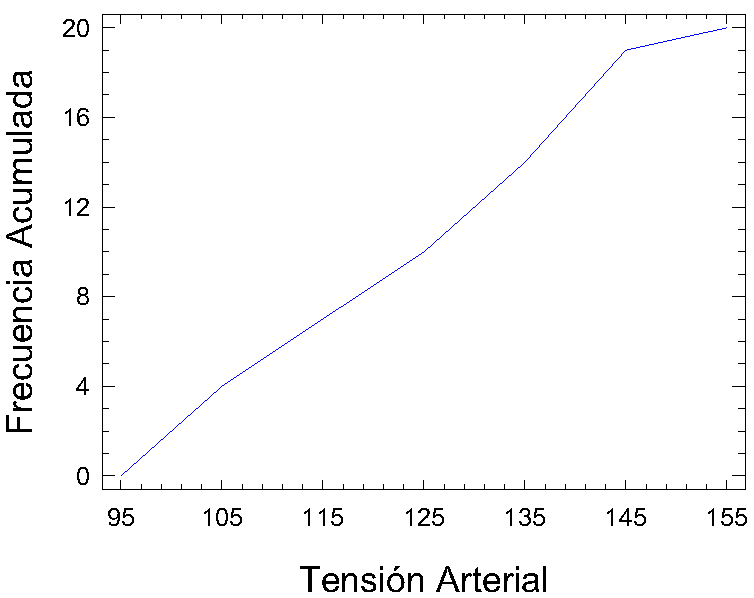
\includegraphics[scale=0.6]{img/poligono-tension-des-37}
\end{center}

\item El coeficiente de asimetría se calcula mediante la fórmula 
\[g_1=\frac{\sum (x-\bar{x})^3n_i/n}{s^3}.\]
A partir de la tabla anterior, calculamos los estadísticos necesarios: 
\[
\begin{array}{|c|r|r|r|r|}
\hline
   X  & \multicolumn{1}{c|}{x_i} & \multicolumn{1}{c|}{n_i} & \multicolumn{1}{c|}{x_in_i} & \multicolumn{1}{c|}{x_i^2n_i}\\
\hline\hline
  [95,105)  &  100  &   4       & 400 & 40000\\
\hline
 [105,115)  &  110 &    3       & 330 & 36300 \\
\hline
 [115,125) &  120 &    3       & 360 &  43200\\
\hline
 [125,135) &  130 &    4       & 520 & 67600 \\
\hline
 [135,145) &  140 &    5       & 700 & 98000 \\
\hline
 [145,155) &  150 &     1       & 150 & 22500\\
\hline
\hline
\textrm{Sumas} & & 20 & 2460 & 307600\\
\hline
\end{array}
\]

\begin{align*}
\bar{x} & = \frac{\sum x_in_i}{n}=\frac{2460}{20}=123,\\
s^2 & =\frac{\sum x_i^2n_i}{N}-\bar{x}^2= \frac{307600}{20}-123^2=251,\\
s & =\sqrt{251}=15.84.
\end{align*}

Por último calculamos el coeficiente de asimetría
\[
\begin{array}{|c|r|r|r|r|}
\hline
   X  & \multicolumn{1}{c|}{x_i} & \multicolumn{1}{c|}{n_i} & \multicolumn{1}{c|}{x_i-\bar{x}} & \multicolumn{1}{c|}{(x_i-\bar{x})^3n_i}\\
\hline\hline
  [95,105)  &  100  &   4       & -23 & -48668\\
\hline
 [105,115)  &  110 &    3       & -13 & -6591 \\
\hline
 [115,125) &  120 &    3       & -3 &  -81\\
\hline
 [125,135) &  130 &    4       & 7 & 1372 \\
\hline
 [135,145) &  140 &    5       & 17 & 24565 \\
\hline
 [145,155) &  150 &     1       & 27 & 19683\\
\hline
\hline
\textrm{Sumas} & & 20 &  & -9720\\
\hline
\end{array}
\]

\[
g_1=\frac{\sum (x-\bar{x})^3n_i/n}{s^3}=\frac{-9720/20}{15.84^3}=-0.12.
\]
Esto indica que la distribución es ligeramente asimétrica a la izquierda.

\item El tercer decil $D_3$ tiene frecuencia absoluta acumulada $N_{D_3}=3n/10=3\cdot 20/10=6$, y mirando en la columna de frecuencias absolutas acumuladas comprobamos que corresponderá a un individuo de la clase $[105,115)$. Interpolando en dicho intervalo tenemos que que el tercer decil es
\[ D_3=105+\frac{6-4}{3}10=111,67,
\]
lo cual indica que  el 30\% de la población tiene un tensión inferior a 111.67.

\item Llamemos $a$ y $b$ a las variables que miden las tensiones de las ciudades A y B respectivamente. Las tensiones serán más homogéneas en la ciudad que haya menos dispersión. Para comparar las dispersiones de ambas poblaciones utilizamos el coeficiente de variación que no depende de las unidades. Calculamos los estadísticos necesarios trabajando directamente desde la muestra sin agrupar:
\begin{align*}
\bar{a} & = \frac{\sum a_{i}}{n}=\frac{135+\cdots+136}{10}=\frac{1301}{10}=130.1,  \\
s_{a}^2 & = \frac{\sum a_{i}^2}{n}-\bar{a}^2 =
\frac{135^2+\cdots+136^2}{10}-130.1^2=\frac{171459}{10}-16926.01=219.89,  \\
s_{a} & = \sqrt{219.89}=14.83,  \\
cv_a &=\frac{s_a}{|\bar{a}|}=\frac{14.83}{130.1}=0.1139,\\
\bar{b} & = \frac{\sum b_{j}}{n}=\frac{128+\cdots+98}{10}=
\frac{1161}{10}=116.1,  \\
s_{b}^2 & = \frac{\sum b_{j}^2}{n}-\bar{b}^2 =
\frac{128^2+\cdots+98^2}{10}-116.1^2=\frac{136689}{10}-13479.21=189.69,  \\
s_{b} & = \sqrt{189.69}=13.77,  \\
cv_b &=\frac{s_b}{|\bar{b}|}=\frac{13.77}{116.1}=0.1186.
\end{align*}
Así pues, comparando los coeficientes de variación en ambas ciudades comprobamos que son prácticamente iguales aunque es un poco menor la dispersión en la ciudad A por lo que las tensiones serán un poco más homogéneas.
\end{enumerate}
}


\newproblem{des-38}{gen}{*}
%ENUNCIADO
{En un grupo de alumnos se ha medido el número de días que faltaron a clase una muestra de alumnos de primer año y otra de alumnos repetidores, obteniendo:
\[
\begin{array}{lcccccccc}
\mbox{Primer año:}  & 8 & 2 & 3  & 2  & 1  & 4 & 0 & 3 \\
\mbox{Repetidores:} & 4 & 6 & 20 & 12 & 16 & 8 & 5 &   \\
\end{array}
\]
Se pide:
\begin{enumerate}
\item Calcular la mediana en ambos casos.
\item ¿En cuál de las dos muestras hay menos dispersión?
\item ¿Comparar el apuntamiento de ambas muestras?
\end{enumerate}
}
%SOLUCIÓN
{\begin{enumerate}
\item $Me_{x}=2.5$ y $Me_{y}=8$.
\item $cv_x =0.7862$ y $cv_y =0.5538$, hay menos dispersión en los alumnos repetidores. 
\item $g_{2_x} =0.703$ y $g_{2_y} =-1.125$ lo que indica que la distribución de los alumnos de primer año es leptocúrtica y la de los repetidores platicúrtica.
\end{enumerate}
}
%RESOLUCIÓN
{Llamemos $X$ a la variable que mide el número de días que faltaron los alumnos de primer año, e $Y$ al de los alumnos repetidores
\begin{enumerate}
\item Para calcular la mediana primero ordenamos los datos de ambas muestras:
\[
\begin{array}{lcccccccc}
\mbox{Primer año:}  & 0 & 1 & 2  & 2  & 3  & 3 & 4 & 8 \\
\mbox{Repetidores:} & 4 & 5 & 6 & 8 & 12 & 16 & 20 &   \\
\end{array}
\]
En el primer caso, como el tamaño de la muestra es par, habrá dos valores que estarán en el centro de la distribución, que serán los que ocupen la posiciones $n/2=8/2=4$ y $n/2+1=5$, es decir, los valores 2 y 3, de modo que la mediana es su media:
\[
Me_{x}=\frac{2+3}{2}=2.5.
\]
En el segundo caso, como el tamaño muestral es impar, sólo habrá un valor central que será el que ocupe la posición $(n+1)/2=8/2=4$, es decir, el valor 8, y por tanto $Me_{y}=8$.

\item Para compara la dispersión de ambas muestras tenemos que calcular el coeficiente de variación, y para ello, previamente hay que calcular la media y la desviación típica de cada muestra:
\begin{align*}
\bar{x} & = \frac{\sum x_{i}}{n}=\frac{8+\cdots+3}{8}=\frac{23}{8}=2.875,  \\
s_{x}^2 & = \frac{\sum x_{i}^2}{n}-\bar{x}^2 =
\frac{8^2+\cdots+3^2}{8}-2.875^2=\frac{107}{8}-8,2656=5.1094,  \\
s_{x} & = \sqrt{5.1094}=2.2604,  \\
cv_x &=\frac{s_x}{|\bar{x}|}=\frac{2.2604}{2.875}=0.7862,\\
\bar{y} & = \frac{\sum y_{j}}{n}=\frac{4+\cdots+5}{7}=
\frac{71}{7}=10.143,  \\
s_{y}^2 & = \frac{\sum y_{j}^2}{n}-\bar{y}^2 =
\frac{4^2+\cdots+5^2}{7}-10.143^2=\frac{941}{7}-102.8804=31.5510,  \\
s_{y} & = \sqrt{31.5510}=5.617,  \\
cv_y &=\frac{s_y}{|\bar{y}|}=\frac{5.617}{10.143}=0.5538.
\end{align*}
Así pues, como el coeficiente de variación es menor en $Y$, hay menos dispersión el grupo de los repetidores.

\item El coeficiente de apuntamiento en ambas muestras es
\begin{align*}
g_{2_x} &=\frac{\sum (x_i-\bar{x})^4}{ns_x^4}-3= \frac{(8-2.875)^4+\cdots + (3-2.875)^4}{8\cdot 2.2604^4}-3=\frac{773.3379}{208.8484}-3=0.703,\\
g_{2_y} &=\frac{\sum (y_j-\bar{y})^4}{ns_y^4}-3= \frac{(4-10.143)^4+\cdots + (5-10.143)^4}{7\cdot 5.617^4}-3=\frac{13068.6239}{6968.1218}-3=-1.125.
\end{align*}
Por tanto, la primera muestra tiene un apuntamiento mayor de lo normal (leptocúrtica) mientras que la segunda muestra tiene un apuntamiento bastante menor de lo normal (platicúrtica). 
\end{enumerate}
}


\newproblem*{des-39}{nut}{*}
%ENUNCIADO
{Al realizar un estudio sobre el peso de las mujeres mayores de 30 años en una determinada población, se obtuvieron los siguientes datos:
\begin{center}
72 -- 66 -- 51 -- 87 -- 65 -- 57 -- 73 -- 84 -- 67 -- 78 \\
58 -- 62 -- 75 -- 56 -- 68 -- 74 -- 57 -- 65 -- 73 -- 67
\end{center}
Realizar un estudio descriptivo agrupando los datos en 4 clases de amplitud 10 comenzando en el 50, que incluya:
\begin{enumerate}
\item Histograma de frecuencias absolutas y frecuencias absolutas acumuladas y los correspondientes polígonos.
\item Rango intercuartílico e interpretación.
\item Estudiar la representatividad de la media.
\end{enumerate}
}


\newproblem*{des-40}{nut}{*}
%ENUNCIADO
{Se realiza un estudio sobre el nivel de colesterol en sangre de los trabajadores de una empresa que utilizan habitualmente el comedor de la misma. Los resultados fueron los siguientes:
\begin{center}
214 - 205 - 197 - 204 - 186 - 192 - 216 - 176 - 192 - 196\\
207 - 182 - 218 - 203 - 194 - 176 - 203 - 214 - 188 - 198 
\end{center}
Se pide:

\begin{enumerate}
\item Obtener la distribución de frecuencias agrupadas en clases de amplitud 10, comenzando en 170.
\item Dibujar el histograma y el polígono de frecuencias.
\item Calcular el coeficiente de variación de Pearson e interpretar los resultados.
\item Calcular el rango intercuartílico.
\end{enumerate}
}


\newproblem{des-41}{psi}{}
%ENUNCIADO
{En un grupo de alumnos universitarios se realiza un estudio sobre la velocidad de lectura.
Para ellos se les dio a leer un texto de un periódico y se contó el número de palabras que leyeron en un minuto, obteniendo los siguientes resultados:
\begin{center}
286 -- 242 -- 185 -- 244 -- 296 -- 211 -- 233 -- 179 -- 190 -- 274 \\
255 -- 222 -- 260 -- 216 -- 204 -- 247 -- 232 -- 257 -- 196 -- 261
\end{center}
Se pide:
\begin{enumerate}
\item Construir la tabla de frecuencias agrupando en intervalos de amplitud 25 comenzando en 175.
\item Calcular las medidas de tendencia central. ¿Es representativa la media?
\item Calcular el coeficiente de apuntamiento e interpretarlo.
\end{enumerate}
}
%SOLUCIÓN
{\begin{enumerate}[start=2]
\item $\bar{x}=233.75$, $Med=235$, $Mod= [225,250)$ y $[250-275]$. $s^2=1017.19$, $s=31.89$ y $cv=0.14$ lo que indica que hay poca dispersión y la media es muy representativa.
\item $g_2=-1.1$ de manera que la distribución es bastante platicúrtica. 
\end{enumerate}
}
%RESOLUCIÓN
{}


\newproblem*{des-42}{amb}{*}
%ENUNCIADO
{Una piscifactoría realiza un estudio para determinar si una especie de pez está en peligro extinción en los ríos de una región.
Para ello se midió el número de peces en 12 sitios diferentes obteniendo los siguientes resultados en unidades por hectómetro cúbico:
\begin{center}
  16 -- 11 -- 14 -- 18 -- 21 -- 27 -- 21 -- 15 -- 22 -- 12 -- 2 -- 19
\end{center}
Se pide:
\begin{enumerate}
\item Dibujar el diagrama de cajas y eliminar de la muestra los datos atípicos si existen.
\item Calcular las medidas de tendencia central. ¿Cuál de ellas es más representativa?
\item Calcular el coeficiente de apuntamiento e interpretarlo.
\end{enumerate}
}


\newproblem*{des-43}{gen}{*}
%ENUNCIADO
{Dado el siguiente polígono correspondiente a una muestra de 60 individuos
\begin{center}
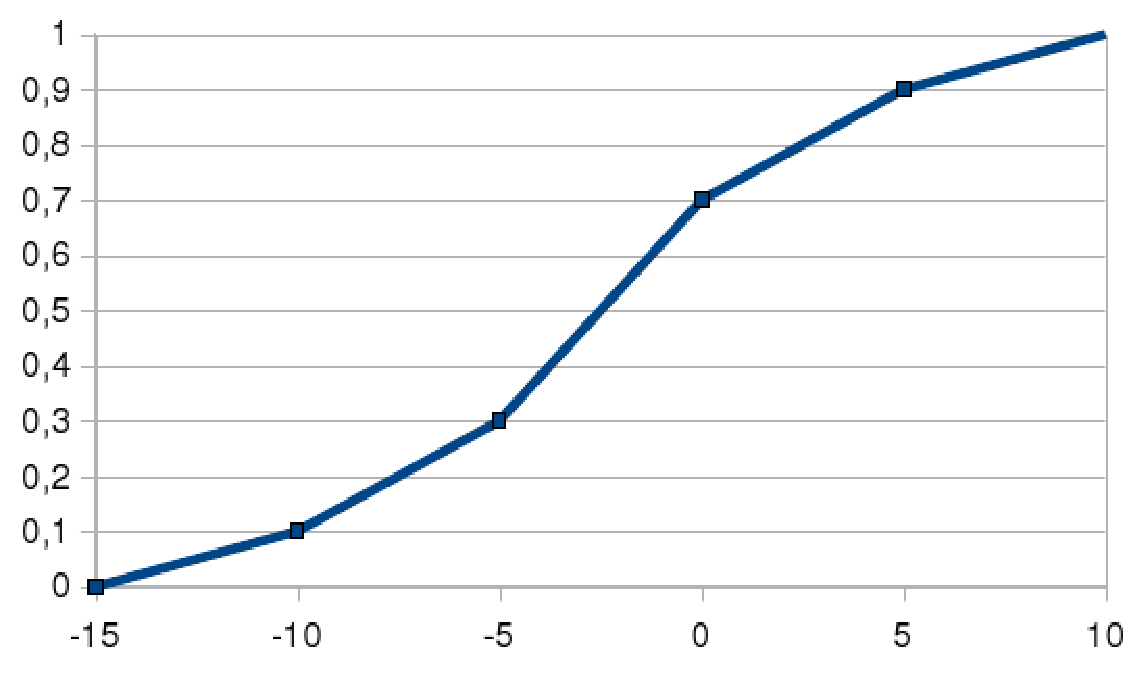
\includegraphics[scale=0.5]{img/poligono-acumuladas-des-43}
\end{center}
Calcular:
\begin{enumerate}
\item Tabla de frecuencias
\item Coeficiente de variación. ¿Se puede decir que hay mucha dispersión?
\item Decil 7.
\item Coeficiente de asimetría e interpretarlo.
\end{enumerate}
}


\newproblem*{des-44}{amb}{*}
%ENUNCIADO
{La siguiente tabla muestra los datos de emisiones de CO$_2$ y CH$_4$ (en Kg/hab) y el producto interior bruto per cápita (en miles US\$) de varios países en el último año:
\[
\begin{array}{|l|r|r|r|}
\hline
\mbox{País} & \mbox{CO}_2 & \mbox{CH}_4 & \mbox{PIB}\\
\hline\hline
\mbox{Austria}     & 7.60 & 0.97 & 38.40\\ \hline
\mbox{España}      & 6.73 & 0.81	& 30.12\\ \hline
\mbox{Francia}     & 5.71 & 0.94	& 33.19\\ \hline
\mbox{EEUU}        &19.40 & 1.72	&	45.84\\ \hline
\mbox{Alemania}    & 9.80 & 0.83	& 34.18\\ \hline
\mbox{Canadá}      &15.60 & 3.08	& 38.43\\ \hline
\mbox{Italia}      & 7.29 & 0.58	& 30.44\\ \hline
\mbox{Japón}       &	9.44 & 0.16	& 33.58\\ \hline
\mbox{Australia}   &17.48 & 6.36	& 36.26\\ \hline
\mbox{Reino Unido} & 8.99 & 0.76	& 35.13\\ \hline
\end{array}
\qquad
\begin{array}{|l|r|r|r|}
\hline
\mbox{País} & \mbox{CO}_2 & \mbox{CH}_4 & \mbox{PIB}\\
\hline\hline
\mbox{Bolivia}     & 1.05 & 3.44	& 40.13\\ \hline
\mbox{Niger}       &	0.1	 & 0.12	&	 0.67\\ \hline
\mbox{Senegal}     &	0.35 & 0.76 &  1.69\\ \hline
\mbox{Pakistán}    & 0.65 & 0.59	&  2.59\\ \hline
\mbox{Filipinas}   &	0.83 & 0.46	&  3.38\\ \hline
\mbox{Perú}        & 0.94 & 0.75	&  7.80\\ \hline
\mbox{Túnez}      & 2.17 & 0.48	&  7.47\\ \hline
\mbox{Nepal}       & 0.13 & 0.90	&  1.21\\ \hline
\mbox{Nicaragua}   & 0.7	 & 0.32	&  2.62\\ \hline
\mbox{Mauritania}  & 0.97 & 0.85	&  2.01\\ \hline
\end{array}
\]
Se pide:
Agrupar los datos de CH$_4$ en 5 clases desde el 0 hasta el 2 y calcular:
\begin{enumerate}
\item Media, varianza y coeficiente de variación. ¿Existe mucha dispersión? Justificar la respuesta.
\item Calcular el Rango Intercuartílico e interpretarlo.
\item Tipificar los datos y calcular el coeficiente de asimetría e interpretarlo.
\end{enumerate}
}


\newproblem{des-45}{amb}{}
%ENUNCIADO
{Se realizó una encuesta a 40 personas de más de 70 años sobre el número de medicamentos distintos que tomaban habitualmente.
El resultado de dicha encuesta fue el siguiente:
\begin{center}
3 -- 1 -- 2 -- 2 -- 0 -- 1 -- 4 -- 2 -- 3 -- 5 -- 1 -- 3 -- 2 -- 3 -- 1 -- 4 -- 2 -- 4 -- 3 -- 2 \\
3 -- 5 -- 0 -- 1 -- 2 -- 0 -- 2 -- 3 -- 0 -- 1 -- 1 -- 5 -- 3 -- 4 -- 2 -- 3 -- 0 -- 1 -- 2 -- 3
\end{center}
Se pide:
\begin{enumerate}
\item Obtener la distribución de frecuencias de la muestra.
\item Dibujar el diagrama de barras y el polígono de frecuencias asociados.
\item Dibujar el diagrama de frecuencias acumuladas.
\item Calcular la media aritmética, la mediana y la moda.
\item Calcular la varianza y la desviación típica.
\item Calcular el coeficiente de variación de Pearson.
\end{enumerate}
}
%SOLUCIÓN
{\begin{enumerate}[start=4]
\item $ \bar{x} = 2.225$, $Med =2$ y $Mod= 2$.
\item $s^2 = 1.974$, $s= 1.405$.
\item $cv = 0.632$.
\end{enumerate}
}
%RESOLUCIÓN
{}


\newproblem*{des-46}{gen}{*}
%ENUNCIADO
{Se considera la variable estadística agrupada en clases cuya distribución de frecuencias viene dada por la siguiente tabla:
\[
\begin{array}{|c|c|c|c|c|}
\hline
X & n_i & f_i & N_i & F_i\\
\hline
[0,20) & & 0.25 & &  \\
\hline
[20,40) & & 0,3 & & \\
\hline
[40,60) &  &  & &  0,9\\
\hline
[60,80) & 6 & & & \\
\hline
\end{array}
\]

\begin{enumerate}
\item Completar razonadamente la tabla.
\item Hallar el rango intercuartílico e interpretarlo.
\item Hallar el coeficiente de apuntamiento e interpretarlo.
\end{enumerate}
}


\newproblem{des-47}{gen}{*}
%ENUNCIADO
{Se han medido las estaturas, $X$, en metros de 15 individuos, obteniéndose los siguientes sumatorios:
\[
\sum\limits_{i = 1}^{15} {x_i  = 26.40\;} {\rm m}{\rm ,}\;\sum\limits_{i = 1}^{15} {x^2 _i  = 52.45\;{\rm m}^{\rm 2} } ,\;\sum\limits_{i = 1}^{15} {\left( {x_i  - \bar x} \right)^3 }  =  - 8.42\;{\rm m}^3
\]

Se pide:
\begin{enumerate}
\item Calcular media, desviación típica, coeficiente de variación y coeficiente de asimetría de la variable. Interpretar los dos últimos.
\item Si trabajamos con una nueva variable $Y=1.1X-0.2$, ¿cuánto valdrán los estadísticos anteriores? Justificar adecuadamente la respuesta.
\end{enumerate}
}
%SOLUCION
{\begin{enumerate}
\item $\bar x=1.76\; \mbox{m}$, $s^2=0.399\;\mbox{m}^2$, $s=0.631\;\mbox{m}$, $CV=0.359$ (dispersión moderada), $g_1=- 2.234$ (distribución muy asimétrica a la izquierda)
\item $\bar y=1.736$, $s_y=0.694$, $CV_y=0.40$, $g_{1y}=-2.234$.
\end{enumerate}
}
%RESOLUCIÓN
{\begin{enumerate}
\item Teniendo en cuenta los sumatorios que nos dan como datos, y el número total de datos en la muestra ($n=15$), obtenemos:
\begin{align*}
\bar x &= \frac{{\sum {x_i } }}{n} = \frac{{26.40}}{15} = 1.76\; \mbox{m},\\
s ^2  &= \frac{{\sum {x_i ^2 } }}{n} - \bar x^2  = \frac{{52.45}}{15} - 1.76^2  =0.399\;\mbox{m}^2,\\
s &=  + \sqrt {s^2 }  =  + \sqrt {0.399}  = 0.631\;\mbox{m},\\
CV &= \frac{s}{{\left| {\bar x} \right|}} = \frac{{0.631}}{{1.76}} = 0.359 = 35.9,\\
g_1 &= \frac{{\frac{{\sum {\left( {x_i  - \bar x} \right)^3 } }}{n}}}{{s^3 }} = \frac{{\frac{{ - 8.42}}{{15}}}}{{0.631^3 }} =  - 2.234.
\end{align*}

En cuanto a la interpretación del coeficiente de variación, su valor es igual a $0.359$, lo cual indica que la dispersión relativa en torno a la media es considerable (supera el 30\%), por lo que la media no es demasiado representativa de la distribución. Para el coeficiente de asimetría hemos obtenido un valor de $-2.234$, negativo lo cual indica que la distribución presenta cola a la izquierda.

\item Si tenemos una nueva variable obtenida mediante la transformación lineal: $Y=1.1 X -0.2$, le podemos aplicar el teorema que nos dice cuáles serán la nueva media y desviación típica de una variable $Y$ obtenida mediante una transformación lineal aplicada a otra $X$. Este teorema dice que si $Y=aX+b$, entonces $\bar y=a \bar x +b$, y $s_y = \left| a \right| s_x$. Por lo tanto:
\[
\bar y = 1.1 \cdot \bar x - 0.2 = 1.736,\qquad s_y  = 1.1 \cdot s_x  = 0.694.
\]

Con los resultados anteriores, el coeficiente de variación de la nueva variable resulta muy sencillo de calcular:
\[
CV_y = \frac{s_y}{{\left| {\bar y} \right|}} = \frac{{0.694}}{{1.736}} = 0.400 = 40.0\%
\]

Y para el coeficiente de asimetría utilizamos su definición basada en sumatorios:
\begin{align*}
g_{1y}  &= \dfrac{{\dfrac{{\sum {\left( {y_i  - \bar y} \right)^3 } }}{n}}}{{s_y ^3 }} = \dfrac{{\dfrac{{\sum {\left( {1.1 \cdot x_i  - 0.2 - \left( {1.1 \cdot \bar x - 0.2} \right)} \right)^3 } }}{{15}}}}{{\left( {1.1 \cdot s_x } \right)^3 }} =\\
&= \dfrac{{\dfrac{{\sum {\left( {1.1 \cdot x_i  - 1.1 \cdot \bar x} \right)^3 } }}{{15}}}}{{\left( {1.1 \cdot s_x } \right)^3 }} = \dfrac{{\dfrac{{1.1^3 \sum {\left( {x_i  - \bar x} \right)^3 } }}{{15}}}}{{1.1^3 \left( {s_x } \right)^3 }} = \dfrac{{\dfrac{{\sum {\left( {x_i  - \bar x} \right)^3 } }}{{15}}}}{{\left( {s_x } \right)^3 }} = g_{1x}  =  - 2.234.
\end{align*}
que como se puede comprobar no cambia.
\end{enumerate}
}


\newproblem{des-48}{gen}{}
%ENUNCIADO
{Dada la siguiente muestra del número de ingresos en urgencias en un determinado hospital,
\begin{center}
5 -- 7 -- 11 -- 7 -- 4 -- 7 -- 24 -- 7 -- 8 -- 8 -- 9 -- 8 -- 13 -- 7 -- 8 -- 17 -- 7 -- 6
\end{center}
estudiar la asimetría de la muestra y transformar los datos para conseguir una simetría más normal.
}
%SOLUCIÓN
{$\bar x=9.055$ ingresos, $s^2=21.4969$ ingresos$^2$, $s=4.6365$ ingresos y $g_1=2.02$.
Para corregir asimetría tomamos $Y=\ln(X)$ y resulta $\bar y= 2.108$, $s_y^2=0.1668$, $s_y=0.4084$ y $g_1=0.95$.
}
%RESOLUCIÓN
{}


\newproblem{des-49}{psi}{}
%ENUNCIADO
{En un experimento se ha medido el tiempo de respuesta a un determinado estímulo visual en grupo de 16 individuos, obteniendo los siguientes resultados (en centésimas de segundo):
\begin{center}
73, 42, 67, 55, 62, 52, 59, 82, 46, 61, 72, 51, 64, 55, 61.
\end{center}
Comprobar si hay datos atípicos en la muestra. En tal caso, sustituirlos por máximos o mínimos valores normales y hacer un resumen descriptivo de la muestra.
}
%SOLUCIÓN
{Los cuartiles son $C_1=52$ cs, $C_3=67$ cs y $RI=15$ cs. Las vallas son $v_1=29.5$ y $v_2=89.5$, luego no hay datos atípicos. $\bar x=60.13$ cs, $s^2=105.58$ cs$^2$, $s=10.28$ cs, $cv=0.17$, $g_1=0.26$ y $g_2=-0.37$.
}
%RESOLUCIÓN
{}


\newproblem{des-50}{psi}{}
%ENUNCIADO
{En un grupo de operarios se ha medido porcentaje de tareas bien realizadas de dos tipos $A$ y $B$, obteniendo los siguientes resultados:
\begin{center}
\begin{tabular}{ccccccccc}
\% A & 58 & 55 & 36 & 67 & 60 & 31 & 53 & 42\\
\% B & 76 & 81 & 82 & 84 & 80 & 75 & 87 & 79\\
\end{tabular}
\end{center}
Se pide:
\begin{enumerate}
\item Calcular las puntuaciones típicas de cada individuo en ambos tipos de tareas.
\item Teniendo en cuenta la distribuciones de puntuaciones de las tareas, ¿en qué tipo de tareas funciona mejor el primer individuo? ¿Y el último? Justificar la respuesta. 
\end{enumerate}
}
%SOLUCIÓN
{$\bar{x}_A=50.25\%$, $\bar{x}_B=80.5\%$, $s_A^2=138.44\%^2$, $s_B^2=13.75\%^2$, $s_A=11.7\%$ y $s_B=3.71\%$. Las puntuaciones típicas son
\begin{center}
\begin{tabular}{ccccccccc}
\% A & 0.66 & 0.4 & -1.21 & 1.42 & 0.83 & -1.64 & 0.23 & -0.7\\
\% B & -1.21 & 0.13 & 0.4 & 0.94 & -0.13 & -1.48 & 1.75 & -0.4\\
\end{tabular}
\end{center} 
}
%RESOLUCIÓN
{}


\newproblem{des-51}{gen}{}
%ENUNCIADO
{En un cuestionario se ha preguntado a un grupo de individuos por su nivel de estudios (SE: sin estudios, EB: estudios básicos, ES: estudios secundarios, EU: estudios universitarios, ED: estudios de doctorado) obteniendo los siguientes resultados:
\begin{center}
EU, ES, ES, EU, EB, EB, ED, SE, EB, SE, EU, ES, ES, ES, EB,\\
EB, SE, ED, EB, ES, ES, SE, EU, EU, EB, ES, EU, ES, EB, ES 
\end{center}
Se pide:
\begin{enumerate}
\item Construir la tabla de frecuencias y los diagramas asociados.
\item Dar una medida de representatividad.
\item Calcular los cuartiles y el percentil 90.
\end{enumerate}
}
%SOLUCIÓN
{\begin{enumerate}[start=2]
\item $Me=$ES y $Mo=$ES.
\item $C_1=$EB, $C_2=$ES, $C_3=$EU y $P_{90}=$EU.
\end{enumerate}
}
%RESOLUCIÓN
{}


\newproblem{des-52}{fis}{*}
%ENUNCIADO
{El tiempo de recuperación, medido en días, de 10 pacientes con una determinada lesión de rodilla ha sido
\begin{center}
46, 54, 48, 62, 51, 50, 54, 50, 49, 52.
\end{center}
Calcular el coeficiente de asimetría y de apuntamiento e interpretarlos. 
}
%SOLUCIÓN
{$g_1=1.22$ (bastante asimétrica hacia la derecha) y $g_2=1.17$ (bastante leptocúrtica).}
%RESOLUCIÓN
{Llamemos $X$ a la variable que mide el tiempo de recuperación de la lesión de rodilla.
Para calcular el coeficiente de asimetría y de apuntamiento necesitamos calcular primero la media y la desviación típica de la variable. Puesto que son pocos datos ($n=10$), trabajaremos con los datos muestrales sin agrupar.
\begin{align*}
\bar x &= \frac{\sum x_i}{n}=\frac{46+54+\cdots+52}{10}=\frac{516}{10}=51.6,\\
s_x^2 &= \frac{\sum x_i^2}{n}-\bar x^2=\frac{46^2+54^2+\cdots+52^2}{10}-51.6^2=\frac{26802}{10}-2662.56=17.64,\\
s_x &= \sqrt{17.64}=4.2
\end{align*}
El coeficiente de asimetría es
\[ g_1=\frac{\sum(x_i-\bar x)^3/n}{s^3}= \frac{((46-51.6)^3+\cdots+(52-51.6)^3)/10}{4.2^3}=\frac{904.32/10}{74.088}=1.22,
\]
lo que indica que la distribución es bastante asimétrica a la derecha.

El coeficiente de apuntamiento es
\[ g_2=\frac{\sum(x_i-\bar x)^4/n}{s^4}-3= \frac{((46-51.6)^4+\cdots+(52-51.6)^4)/10}{4.2^4}-3=\frac{12975.312/10}{311.1696}-3=1.17,
\]
lo que indica que la distribución es bastante más apuntada de lo normal, es decir, es leptocúrtica.
}


\newproblem{des-53}{nut}{*}
%ENUNCIADO
{ La ingesta calórica durante la comida para un individuo al que se ha hecho un seguimiento estricto durante 15 días, expresada en
kilocalorías, ha sido:
\begin{center}
1121, 1138, 1101, 1025, 1323, 1450, 1005, 1214, 1040, 1321 \\
1225, 1428, 1105, 1202, 1483, 1465, 1362, 1325, 1010, 1311
\end{center}
Agrupar los datos en 5 clases de amplitud 100, comenzando en 1000 kilocalorías, y utilizando dicha agrupación calcular: 
\begin{enumerate}
\item Coeficiente de variación.
\item Rango intercuartílico.
\item Coeficiente de asimetría.
\end{enumerate}
Interpretar los resultados.
}
%SOLUCIÓN
{Llamando $X$ al número de kilocalorías ingeridas al día:
\begin{enumerate}
\item $bar x= 1255$ kcal, $s_x^2=20475$ kcal$^2$, $s_x=143.091$ kcal y $cv_x=0.114$, lo que indica que hay poca dispersión y la media es
muy representativa.
\item $C_1=1125$ kcal, $C_3=1389$ kcal y $RI=255$ kcal.
\item $g_{1}=-0.0878$, lo que indica que la distribución es casi simétrica.
\end{enumerate}
}
%RESOLUCIÓN
{Llamemos $X$ al número de kilocalorías ingeridas al día.
\begin{enumerate}
\item Teniendo en cuenta la agrupación propuesta y lo que se nos pide en los apartados siguientes, la tabla que necesitamos es:

\[
\begin{array}{|c|r|r|r|r|r|r|r|} \hline
\textrm{Intervalos} & \multicolumn{1}{c|}{x_{i}} & \multicolumn{1}{c|}{n_{i}} &
\multicolumn{1}{c|}{N_{i}} & \multicolumn{1}{c|}{x_{i}n_{i}} &
\multicolumn{1}{c|}{x_{i}^{2}n_{i}} & \multicolumn{1}{c|}{x_{i}-\bar x} &
\multicolumn{1}{c|}{(x_{i}- \bar x)^3n_{i}}
\\ \hline
\left[ 1000,1100\right)  & 1050 & 4 & 4 & 4200 &  4410000 & -205 & -34460500
\\ \hline
\left[ 1100,1200\right)  & 1150 & 4 & 8 & 4600 & 5290000 & -105 & -4630500
\\ \hline
\left[ 1200,1300\right)  & 1250 & 3 & 11 & 3750 & 4687500 & -5 & -375
\\ \hline
\left[ 1300,1400\right)  & 1350 & 5 & 16 & 6750 &  9112500 & 95 & 4286875
\\ \hline
\left[ 1400,1500\right)  & 1450 & 4 & 20 & 5800 &  8410000 & 195 & 29659500
\\ \hline
\textrm{Sumas}&  & 20 &  & 25100 &  31910000 & & -5145000
\\ \hline
\end{array}
\]

De todo ello:
\begin{align*}
\bar x& =\dfrac{\sum x_{i}n_{i}}{\sum n_{i}}=\dfrac{25100}{20}=1255\text{ kcal},\\
s_{x}^{2}& =\dfrac{\sum x_{i}^{2}n_{i}}{\sum n_{i}}-\bar x^{2}=\dfrac{31910000}{20}-1255^{2}=20475\text{ kcal}^{2},\\
s_{x}& =+\sqrt{s_{x}^{2}}=143.091\text{ kcal},
\end{align*}
y el coeficiente de variación:
\[
cv_x=\dfrac{s_{x}}{\left| \overline{x}\right| }=0.114
\]
Para su interpretación, teniendo en cuenta que $0.114$ está cercano a 0, la desviación típica será muy pequeña en comparación con la media,
lo cual implica que la media muestral será bastante representativa.

\item El rango intercuartílico es la diferencia entre el tercer cuartil y el primero, así que se hay que calcular el primer y
el tercer cuartil. Para el primero de los cuartiles, teniendo en cuenta que le corresponde una frecuencia acumulada $n/4$, es decir 5, luego
se encuentra el intervalo $\left[ 1100,1200\right)$, y aplicando semejanza de triángulos:
\[
\dfrac{8-4}{1200-1100}=\dfrac{5-4}{C_{1}-1100} \Leftrightarrow C_{1}=1125\text{ kcal}.
\]

De la misma forma pero procediendo con una frecuencia acumulada $3n/4=15$ para $C_{3}$, lo cual indica que se encuentra en el intervalo
$\left[ 1300,1400\right)$:%
\[
\dfrac{16-11}{1400-1300}=\dfrac{15-11}{C_{3}-1300} \Leftrightarrow C_{3}=1380\text{ kcal}.
\]

Por lo tanto el rango intercuartílico vale $RI=C_{3}-C_{1}=1380-1125=255\text{ kcal,}$
\]
cuya interpretación es que entre 1125 kcal y 1380 kcal se encuentran el 50\% de los individuos de la muestra que comen una cantidad media de
kilocalorías (lejos de los ``excesos'' del 25\% que más kilocalorías toman, o de los ``defectos'' del 25\% que menos kilocalorías
ingieren). Se puede observar, así mismo, que estos datos centrales no están muy dispersos.

\item El coeficiente de asimetría es
\[
g_{1}=\dfrac{\dfrac{\sum \left( x_{i}-\bar x\right) ^{3}n_{i}}{N}}{s_{x}^{3}}=\dfrac{\dfrac{-5145000}{20}}{143.091^{3}}=-0.0878,
\]
cuya interpretación es que la distribución es casi simétrica, con una ligera asimetría a la izquierda.
\end{enumerate}
}


\newproblem{des-54}{med}{*}
%ENUNCIADO
{En un laboratorio se ha medido el número de hijos que tuvieron unas ratas que habían seguido un tratamiento de fertilidad, obteniendo los
siguientes resultados:
\begin{center}
7 -- 5 -- 6 -- 6 -- 8 -- 9 -- 10 -- 8 -- 7 -- 6 -- 8 -- 7 -- 9 -- 11 -- 8 -- 7 -- 7 -- 7 -- 6 -- 8
\end{center}

\begin{enumerate}
\item Existen datos atípicos en la muestra? Justificar la respuesta.\\
Nota: En caso de detectarse algn dato atípico, no quitarlo.
\item Calcular los coeficientes de asimetría y apuntamiento e interpretarlos. Se puede concluir que la muestra proviene de una población
normal?
\end{enumerate}
}
%SOLUCIÓN
{\begin{enumerate}
\item El 11 es un dato atípico. 
\item $g_1=0.61$ lo que indica que las distribución es asimétrica hacia la derecha, y $g_2=0.084$, lo que indica que la distribución es un
poco platicúrtica. Como ambos valores están en el intervalo $[-2,2]$ se puede suponer que la muestra viene de una población normal. 
\end{enumerate}
}
%RESOLUCIÓN
{}


\newproblem{des-55}{nut}{*}
%ENUNCIADO
{En un estudio sobre el número de kilocalorías diarias en la dieta de los españoles mayores de edad se han obtenido los siguientes datos, en
una muestra de tamaño 200, separada por sexos:
\begin{center}
\begin{tabular}{|l|c|c|}
\hline
Kilocaloras & Hombres & Mujeres \\
\hline
[1000, 1400) & 1 & 15\\
\hline
[1400, 1800) & 10 & 24\\
\hline
[1800, 2200) & 25 & 28\\
\hline
[2200, 2600) & 34 & 15\\
\hline
[2600, 3000) & 26 & 10\\
\hline
[3000, 3400) & 12 & 0\\
\hline
\end{tabular}
\end{center}

\begin{enumerate}
\item Qué media de consumo de kilocaloras es más representativa de su distribución, la de hombres o la de mujeres? Justificar adecuadamente
la respuesta.
\item Cuánto vale el percentil 90 del consumo de kilocaloras en los hombres?
\item Cuánto vale el coeficiente de apuntamiento de la distribución global, considerando hombres y mujeres? Interpretarlo.
\end{enumerate}
}
%SOLUCIÓN
{Llamando $h$ y $m$ al número de kilocalorías en hombres y mujeres respectivamente:
\begin{enumerate}
\item $\bar h=2407.407$ kcal, $s_h=468.1927$ kcal y $cv_h=0.1945$.\\
$\bar m=1917.391$ kcal  $s_m=484.6802$ kcal y $cv_m=0.2528$.
\item El percentil 90 en los hombres vale $3040$ kcal. 
\item $g_2=-0.73$, lo que indica que la distribución es platicúrtica. 
\end{enumerate}
}
%RESOLUCIÓN
{}



\newproblem{des-56}{gen}{*}
%ENUNCIADO
{En un examen de estadística al que se han presentado 66 alumnos se ha contado el número de exámenes finalizados cada media hora, 
obteniendo el siguiente polígono:
\begin{center}
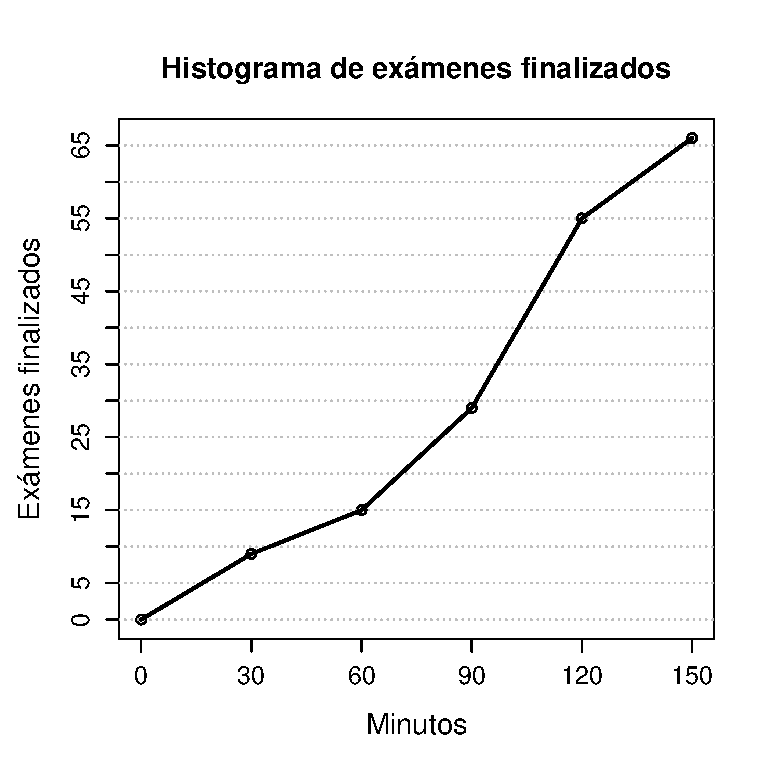
\includegraphics[scale=0.8]{img/poligono-des-56}
\end{center}
Se pide:
\begin{enumerate}
\item ¿Existe mucha dispersión en la muestra? Justificar la respuesta.
\item ¿Cuánto tiempo tiene que pasar para que hayan finalizado el examen la mitad de los alumnos?
\item Estudiar la asimetría de la distribución.  
\end{enumerate}
}
%SOLUCIÓN
{\begin{enumerate}
\item $\bar x= 85.9091$ min, $s^2 =1408.2645$ min$^2$, $s= 37.5268$ min y $cv= 0.4368$, luego existe una dispersión moderada.
\item $Me = 94.6154$ min.
\item $g_1= -0.618$, lo que indica que la distribución es asimétrica hacia la izquierda. 
\end{enumerate}
}
%RESOLUCIÓN
{\begin{enumerate}
\item Para ver si la muestra tienen mucha dispersión hay que calcular la desviación típica o el coeficiente de variación, pero antes necesitamos
conocer las frecuencias absolutas de cada clase. En la tabla que nos dan aparece el número de exámenes finalizados para cada instante, que es,
en realidad, la frecuencia absoluta acumulada. A partir de ella se puede obtener facilmente la frecuencia absoluta de cada clase simplemente
restando a la frecuencia absluta acumulada de la clase siguiente la de la clase actual. Así se obtiene la siguiente tabla de frecuencias. 
\[
\begin{array}{rrrr}
  \hline
 & x_i & n_i & N_i \\ 
  \hline
(0,30] & 15 & 9 & 9 \\ 
  (30,60] & 45 & 6 & 15 \\ 
  (60,90] & 75 & 14 & 29 \\ 
  (90,120] & 105 & 26 & 55 \\ 
  (120,150] & 135 & 11 & 66 \\ 
   \hline
\end{array}\]

Para calcular la desviación típica se añaden nuevas columnas a la tabla de frecuencias con los cálculos necesarios:
\[
\begin{array}{rrrrr}
  \hline
 & x_i & n_i & x_in_i & x_i^2n_i \\ 
  \hline
(0,30] & 15 & 9 & 135 & 2025 \\ 
  (30,60] & 45 & 6 & 270 & 12150 \\ 
  (60,90] & 75 & 14 & 1050 & 78750 \\ 
  (90,120] & 105 & 26 & 2730 & 286650 \\ 
  (120,150] & 135 & 11 & 1485 & 200475 \\ 
  \sum &  & 66 & 5670 & 580050 \\ 
   \hline
\end{array}\]

A partir de la tabla calculamos los estadísticos que se piden:
\begin{align*}
\bar x &= \frac{\sum x_in_i}{n_x} = \frac{5670}{66} = 85.9091,\\
s^2 & = \frac{\sum x_i^2n_i}{n_x}-\bar x^2 = \frac{580050}{66}-7380.3735 = 1408.2645,\\
s & = \sqrt{1408.2645} = 37.5268,\\
cv & = \frac{s}{|\bar x|} = \frac{37.5268}{|85.9091|} = 0.4368.
\end{align*}
Lo que indica que hay una dispersión moderada. 

\item El tiempo que transcurra hasta que hayan finalizado el examen la mitad de los alumnos es precisamente la mediana.
La frecuencia absoluta acumulada correspondiente a la mediana es $66/2 = 33$ de modo que la mediana cae en la clase $[90,120)$, e interpolando en esta clase se obtiene
\[
Me = 90+\frac{33-29}{26}30 = 94.6154 \text{ min}.
\]

\item Para estudiar la asimetría de la muestra se calcula el coeficiente de asimetría. Para ello se añade una nueva columna a la tabla de
frecuencias con las desviaciones a la media al cubo:
\[
\begin{array}{rrrrr}
  \hline
 & x_i & n_i & x_i-\bar x & (x_i-\bar x)^3n_i \\ 
  \hline
(0,30] & 15 & 9 & -70.9091 & -3208841.4726 \\ 
  (30,60] & 45 & 6 & -40.9091 & -410781.3674 \\ 
  (60,90] & 75 & 14 & -10.9091 & -18175.8077 \\ 
  (90,120] & 105 & 26 & 19.0909 & 180906.0856 \\ 
  (120,150] & 135 & 11 & 49.0909 & 1301355.3719 \\ 
  \sum &  & 66 &  & -2155537.1901 \\ 
   \hline
\end{array}\]

A partir de la tabla calculamos los estadísticos que se piden:
\[
g_{1} &= \frac{\sum (x_i-\bar x)^3 n_i/n_x}{s_x^3} = \frac{-2155537.1901/66}{37.5268^3} = -0.618.
\]

Lo que indica que la distribución es asimétrica hacia la la izquierda. 
\end{enumerate}
}


% Author Alfredo Sánchez Alberca (asalber@ceu.es)

\newproblem{reg-1}{gen}{}
% ENUNCIADO
{Dada la siguiente tabla de correlación:
\begin{center}
\begin{tabular}{|c||c|c|c|}
\hline
$X\setminus Y$ & 1 & 2 & 3 \\ \hline\hline
$\left[ -2,2\right) $ & 3 & 6 & 1 \\ \hline
$\left[ 2,6\right) $ & 4 & 7 & 3 \\ \hline
$\left[ 6,10\right) $ & 5 & 3 & 0 \\ \hline
\end{tabular}
\end{center}

Determinar:
\begin{enumerate}
\item  Las distribuciones marginales. Media, Moda y Mediana.
\item  Rectas de Regresión.
\item  Coeficiente de correlación lineal. Interpretar el resultado.
\end{enumerate}
}
%SOLUCIÓN
{}
%RESOLUCIÓN
{}


\newproblem{reg-2}{med}{}
%ENUNCIADO
{Una compañía de asistencia sanitaria hace un estudio del número de veces que, durante el último trimestre, han acudido sus asegurados a consultas de especialistas, en función de su edad. En la siguiente tabla se reflejan los resultados obtenidos:
\begin{center}
\begin{tabular}{|c||c|c|c|c|c|}
\hline
$\mbox{Edad}\setminus \mbox{Cons.}$ & 0 & 1 & 2 & 3 & 4 \\ \hline\hline
$\left[ 30,40\right) $ & 6 & 2 & 2 & 0 & 0  \\ \hline
$\left[ 40,50\right) $ & 4 & 3 & 6 & 4 & 1 \\ \hline
$\left[ 50,60\right) $ & 0 & 2 & 4 & 5 & 3 \\ \hline
$\left[ 60,70\right) $ & 0 & 0 & 3 & 4 & 5 \\ \hline
$\left[ 70,80\right) $ & 0 & 0 & 0 & 4 & 6 \\ \hline
\end{tabular}
\end{center}

Se pide:
\begin{enumerate}
\item Recta de regresión del número de consultas sobre la edad.
\item Coeficiente de correlación e interpretarlo.
\item ¿Cuántas consultas se espera que realice una persona de 52 años?¿Es fiable esta predicción?
\end{enumerate}
}
%SOLUCIÓN
{}
%RESOLUCIÓN
{}


\newproblem{reg-3}{far}{}
%ENUNCIADO
{Se determina la pérdida de actividad que experimenta un medicamento desde el momento de su fabricación a lo largo del
tiempo, obteniéndose el siguiente resultado: 

\begin{center}
\begin{tabular}{|c|c|c|c|c|c|}
\hline
Tiempo (en años) & 1 & 2 & 3 & 4 & 5 \\ \hline
Actividad restante (\%) & 96 & 84 & 70 & 58 & 52 \\ \hline
\end{tabular}
\end{center}

Se pide:
\begin{enumerate}
\item Calcular la recta de regresión de la actividad sobre el tiempo transcurrido.
\item Según el modelo lineal, ¿cuánto tiempo debe pasar para que la actividad del fármaco sea del 80\%? 
¿Cuándo será nula la actividad?
\end{enumerate}
}
%SOLUCIÓN
{Llamando $T$ al tiempo y $A$ a la actividad del fármaco:
\begin{enumerate}
\item $\bar t=3$ años, $\bar a=72\%$, $s_t^2=2$ años$^2$, $s_a^2=264\%^2$, $s_{ta}=-22.8$ años$\cdot\%$.\\
Recta de regresión de actividad sobre tiempo: $a=-11.4t+106.2$.
\item Recta de regresión de tiempo sobre actividad: $t=-0.086a+9.2182$.\\
$t(80)=2.3091$ años y $t(0)=9.2182$ años.
\end{enumerate}
}
%RESOLUCIÓN
{}


\newproblem{reg-4}{amb}{}
%ENUNCIADO
{Las temperaturas medias mensuales (en $^\circ$C) y las precipitaciones totales mensuales (en mm) durante el año 2001 en Madrid fueron:
\begin{center}
\begin{tabular}{|l|r|r|r|r|r|r|r|r|r|r|r|r|}
\cline{2-13}
\multicolumn{1}{c|}{} &    Ene &    Feb &    Mar &    Abr &    May &    Jun &    Jul &    Ago &    Sep &    Oct &    Nov &    Dic \\
\hline
Temp.               &  $7.2$ &  $8.4$ & $12.2$ & $13.7$ & $16.7$ & $23.3$ & $24.2$ & $25.5$ & $20.4$ & $16.2$ &  $8.1$ &  $4.2$ \\
\hline
Prec.                & $73.6$ & $31.7$ & $72.1$ & $20.7$ & $37.1$ & $3.8$ & $3.3$ & $1.5$ & $23.1$ & $67.0$ & $12.4$ & $18.0$ \\
\hline
\end{tabular}
\end{center}
¿Existe relación lineal entre las precipitaciones y la temperatura?
De acuerdo a esta relación, ¿qué cantidad de precipitaciones se espera que haya un mes con una temperatura media de 15$^\circ$C?¿Es fiable esta predicción?
}
%SOLUCIÓN
{}
%RESOLUCIÓN
{}


\newproblem{reg-5}{gen}{}
% ENUNCIADO
{Se ha realizado un estudio comparativo de las puntuaciones obtenidas por los alumnos en un test de ingreso en la
universidad ($X$), y el número de asignaturas aprobadas en el primer curso ($Y$). Los resultados obtenidos se expresan en
la siguiente tabla:

\begin{center}
\begin{tabular}{|c||c|c|c|c|c|}
\hline
$X\setminus Y$ & 0 & 1 & 2 & 3 & 4 \\ \hline\hline
$\left[ 0,10\right) $ & 2 & 2 & 1 & 0 & 0 \\ \hline
$\left[ 10,20\right) $ & 1 & 1 & 2 & 2 & 0 \\ \hline
$\left[ 20,30\right) $ & 0 & 1 & 3 & 4 & 1 \\ \hline
$\left[ 30,40\right) $ & 0 & 0 & 2 & 2 & 6 \\ \hline
\end{tabular}
\end{center}

Se desea calcular:
\begin{enumerate}
\item Recta de regresión de $X$ sobre $Y.$
\item Coeficiente de correlación e interpretación del mismo.
\item Si la universidad en cuestión sólo contara con alumnos que al menos logren aprobar dos asignaturas, ¿qué número
de preguntas respondidas correctamente exigirá en el test?
\end{enumerate}
}
%SOLUCIÓN
{
\begin{enumerate}
\item $\bar x=23$ puntos, $\bar y=2.4$ asignaturas, $s_x^2=116$ puntos$^2$, $s_y^2=1.5733$ asignaturas$^2$,
$s_x=10.7703$ puntos, $s_y=1.2453$ asignaturas y $s_{xy}=9.8$ puntos$\cdot$asignaturas.\\
Recta de regresión de $X$ sobre $Y$: $x=6.2288y+8.0508$.
\item $r=0.73$, lo que quiere decir que hay buena relación lineal entre las puntuaciones y las asignaturas aprobadas y
además es creciente (a mayor puntuación en el test, más asignaturas aprobadas).
\end{enumerate}
}
%RESOLUCIÓN
{}


\newproblem{reg-6}{nut}{*}
%ENUNCIADO
{La tabla siguiente representa la distribución bidimensional de frecuencias de una muestra de 80 personas en un estudio sobre la relación entre el nivel de colesterol en sangre ($X$) en mg/dl y la tensión arterial máxima ($Y$) en mmHg.
\[
\begin{array}{|c||c|c|c||c|}
\hline
X\setminus Y & [110,130) & [130,150) & [150,170) & n_x \\
\hline\hline
[170,190)   &           &     4     &           & 12\\
\hline
[190,210)   &    10     &    12     &     4     &   \\
\hline
[210,230)   &     7     &           &     8     &   \\
\hline
[230,250)   &     1     &           &           & 18\\
\hline\hline
n_y          &           &    30     &    24    &    \\
\hline
\end{array}
\]
Se pide:
\begin{enumerate}
\item Completar la tabla.
\item Calcular la recta de regresión del nivel de colesterol sobre la tensión.
\item Usar el modelo lineal para predecir el colesterol esperado para una persona con una tensión arterial de 160 mmHg.
\item Según el modelo lineal, ¿cuál es la tensión arterial máxima esperada para una persona cuyo nivel de colesterol es 270 mg/dl.
\end{enumerate}

Usar las siguientes sumas:
$\sum x_i=16960$ mg/dl, $\sum y_j=11160$ mmHg, $\sum x_i^2=3627200$ (mg/dl)$^2$, $\sum y_j^2=1576800$ mmHg$^2$ y
$\sum x_iy_j=2378800$ mg/dl$\cdot$mmHg.
}
%SOLUCIÓN
{
\begin{enumerate}
\item Tabla de frecuencias
\[
\begin{array}{|c||c|c|c||c|}
\hline
X\setminus Y & [110,130) & [130,150) & [150,170) & n_x \\
\hline\hline
[170,190)   &     8     &     4     &     0     & 12 \\
\hline
[190,210)   &    10     &    12     &     4     & 26 \\
\hline
[210,230)   &     7     &     9     &     8     & 24 \\
\hline
[230,250)   &     1     &     5     &    12     & 18 \\
\hline\hline
n_y          &   26     &    30     &    24     & 80 \\
\hline
\end{array}
\]
\item $\bar x=212$ mg/dl, $\bar y=139.5$ mmHg, $s_x^2=396$ (mg/dl)$^2$, $s_y^2=249.75$ mmHg$^2$ y $s_{xy}=161$
mg/dl$\cdot$mmHg. Recta de regresión del nivel de colesterol sobre la tensión arterial: $x=122.0721+0.6446y$. 
\item  $x(160)=225.2152$ mg/dl.
\item Recta de regresión de la tensión arterial sobre el colesterol: $y=0.4066x+53.3081$.\\
$y(270)=163.0808$ mmHg.
\end{enumerate}
}
%RESOLUCIÓN
{}


\newproblem{reg-7}{nut}{*}
%ENUNCIADO
{En un centro dietético se está probando una nueva dieta de adelgazamiento en una muestra de 12 individuos. Para cada
uno de ellos se ha medido el número de días que lleva con la dieta y el número de kilos perdidos desde entonces,
obteniéndose los siguientes resultados:
\begin{center}
(33 , 3.9), (51 , 5.9), (30 , 3.2), (55 , 6.0), (38 , 4.9), (62 , 6.2),\\
(35 , 4.5), (60 , 6.1), (44 , 5.6), (69 , 6.2), (47 , 5.8), (40 , 5.3)
\end{center}
Se pide:
\begin{enumerate}
\item Dibujar el diagrama de dispersión. Según la nube de puntos, ¿qué tipo de modelo explicaría mejor la relación
entre los días de dieta y los kilos perdidos? 
\item Calcular el modelo lineal y el logarítmico de los kilos perdidos con respecto a los días de dieta.
\item Utilizar el mejor de los modelos anteriores para predecir en número de kilos perdidos tras 40 días de dieta y tras 100 días.
¿Son fiables estas predicciones?
\end{enumerate}
Usar las siguientes sumas ($X$=Días de dieta e $Y$=Peso perdido): $\sum x_i=564$ días, $\sum \log(x_i)=45.8086$
$\log(\mbox{días})$, $\sum y_j=63.6$ kg, $\sum x_i^2=28234$ días$^2$, $\sum \log(x_i)^2=175.6603$ $\log(\mbox{días})^2$, $\sum y_j^2=347.7$ kg$^2$, $\sum x_iy_j=3108.5$ días$\cdot$kg, $\sum \log(x_i)y_j=245.4738$ $\log(\mbox{días})\cdot$kg.
}
%SOLUCIÓN
{Llamando $X$ a los días de dieta, $Y$ a los kg perdidos y $Z=\log X$.
\begin{enumerate}[start=2]
\item $\bar x=47$ días, $\bar y=5.3$ kg, $s_x^2=143.833$ días$^2$, $s_y^2=0.885$ kg$^2$, $s_{xy}=9.942$ días$\cdot$kg.
Modelo lineal: $y=0.069x+2.051$.\\ 
$\bar z=3.82$ $\log(\mbox{días})$, $s_z^2=0.07$ $\log^2(\mbox{días})$, $s_{yz}=0.22$ $\log(\mbox{días})\cdot\mbox{kg}$.\\
Modelo logarítmico: $y=3.4\log y-7.67$. 
\item Modelo lineal: $r^2=0.78$, modelo logarítmico: $r^2=0.86$.\\
Predicciones con el modelo logarítmico: $y(40)=4.86$ kg y $y(100)=7.98$ kg. 
Las predicciones son fiables ya que el coeficiente de determinación es alto, aunque la de 100 días no lo es tanto por estar fuera del rango de valores observados en la muestra. 
\end{enumerate}
}
%RESOLUCIÓN
{}


\newproblem{reg-8a}{far}{*}
%ENUNCIADO
{Al realizar un estudio sobre la dosificación de un cierto medicamento, se trataron 6 pacientes con dosis diarias de 2
mg, 7 pacientes con 3 mg y otros 7 pacientes con 4 mg. De los pacientes tratados con 2 mg, 2 curaron al cabo de 5 días,
y 4 al cabo de 6 días. De los pacientes tratados con 3 mg diarios, 2 curaron al cabo de 3 días, 4 al cabo de 5 días y 1
al cabo de 6 días. Y de los pacientes tratados con 4 mg diarios, 5 curaron al cabo de 3 días y 2 al cabo de 5 días.

Se pide:
\begin{enumerate}
\item Construir la tabla de la distribución conjunta de frecuencias.
\item Obtener las distribuciones de frecuencias marginales y calcular los principales estadísticos para cada variable. 
\item Calcular la covarianza e interpretarla. 
\end{enumerate}
}
%SOLUCIÓN
{Llamando $X$ a la dosis e $Y$ al tiempo de curación:
\begin{enumerate}[start=3]
\item $\bar x=3.05$ mg, $\bar y=4.55$ días, $s_x^2=0.648$ mg$^2$, $s_y^2=1.448$ días$^2$, $s_x=0.805$ mg, $s_y=1.203$
días y $s_{xy}=-0.678$ mg$\cdot$días, lo que indica que hay una relación lineal decreciente. 
\end{enumerate}
}
%RESOLUCIÓN
{}


\newproblem{reg-8b}{far}{*}
%ENUNCIADO
{Al realizar un estudio sobre la dosificación de un cierto medicamento, se trataron 6 pacientes con dosis diarias de 2
mg, 7 pacientes con 3 mg y otros 7 pacientes con 4 mg. De los pacientes tratados con 2 mg, 2 curaron al cabo de 5 días,
y 4 al cabo de 6 días. De los pacientes tratados con 3 mg diarios, 2 curaron al cabo de 3 días, 4 al cabo de 5 días y 1
al cabo de 6 días. Y de los pacientes tratados con 4 mg diarios, 5 curaron al cabo de 3 días y 2 al cabo de 5 días.

Se pide:
\begin{enumerate}
\item Dar el coeficiente de correlación e interpretación.
\item Determinar el tiempo esperado de curación para una dosis de 5 mg diarios.
\end{enumerate}
}
%SOLUCIÓN
{Llamando $X$ a la dosis e $Y$ al tiempo de curación:
\begin{enumerate}
\item $\bar x=3.05$ mg, $\bar y=4.55$ días, $s_x^2=0.648$ mg$^2$, $s_y^2=1.448$ días$^2$, $s_x=0.805$ mg, $s_y=1.203$
días y $s_{xy}=-0.678$ mg$\cdot$días.\\
$r=-0.7$, que quiere decir que hay buena relación lineal entre la dosis y el tiempo de curación, y además es
decreciente (a mayor dosis, menor tiempo de curación).
\item Recta de regresión del tiempo de curación sobre la dosis: $y=-1.046x+7.741$.\\
$y(5)=2.511$ días.
\end{enumerate}
}
%RESOLUCIÓN
{}


\newproblem{reg-9}{nut}{*}
%ENUNCIADO
{Después de tomar un litro de vino se ha medido la concentración de alcohol en la sangre en distintos instantes,
obteniendo:
\[
\begin{tabular}{|c|c|c|c|c|c|c|}
\hline
Tiempo después (minutos) & 30 & 60 & 90 & 120 & 150 & 180 \\ \hline
Concentración (gramos/litro) & 1.6 & 1.7 & 1.5 & 1.1 & 0.7 & 0.2 \\
\hline
\end{tabular}
\]

Se pide:
\begin{enumerate}
\item Calcular la recta de regresión de la concentración en función del tiempo.
\item ¿Qué concentración de alcohol habrá a los 100 minutos?
\item Si la concentración máxima de alcohol en la sangre que permite la ley para poder conducir es 0.8 g/l, ¿cuánto tiempo habrá que esperar después de tomarse un litro de vino para poder conducir sin infringir la ley?
\end{enumerate}
}
%SOLUCIÓN
{}
%RESOLUCIÓN
{}


\newproblem{reg-10}{gen}{}
%ENUNCIADO
{Se consideran dos variables aleatorias $X$ e $Y$ tales que:
\begin{itemize}
\item[--] La recta de regresión de $Y$ sobre $X$ viene dada por la ecuación: $y-x-2=0$.
\item[--] La recta de regresión de $X$ sobre $Y$ viene dada por la ecuación: $y-4x+22=0$.
\end{itemize}
Calcular:
\begin{enumerate}
\item  Valores de $\bar x$ e $\bar y$.
\item  Coeficiente de correlación lineal.
\end{enumerate}
}
%SOLUCIÓN
{
\begin{enumerate}
\item $\bar x=8$ y $\bar y=10$.
\item $r=0.5$.
\end{enumerate}
}
%RESOLUCIÓN
{}


\newproblem{reg-11}{gen}{}
%ENUNCIADO
{En el ajuste rectilíneo a una distribución bidimensional se sabe que $\bar x=2$, $\bar y=1$, y el coeficiente de correlación lineal es 0 ($r=0$).
\begin{enumerate}
\item  Si $x=10$, ¿cuál será el valor interpolado para $y$?.
\item  Si $y=5$, ¿cuál será el valor interpolado para $x$?.
\item  Dibuja las rectas de regresión de $Y$ sobre$X$, y la de $X$ sobre $Y$.
\end{enumerate}
}
%SOLUCIÓN
{
\begin{enumerate}
\item $y(10)=1$.
\item $x(5)=2$.
\end{enumerate}
}
%RESOLUCIÓN
{}


\newproblem{reg-12}{gen}{*}
%ENUNCIADO
{En un estudio para relacionar la longitud de la línea de la vida de la mano izquierda y la duración de la vida de una
persona se han obtenido datos de 50 personas con los siguientes resultados ($X$=longitud de la línea en cm, $Y$=edad al
morir en años):
\[ 
\sum y=3333 \quad \sum y^2=231933 \quad \sum x=459.9 \quad \sum x^2=4308.57 \quad \sum xy=30949. 
\]
A la vista de estos resultados, ¿cuanto vivirá, por termino medio, una persona con una línea de longitud 7.5 cm?
¿Es fiable esta estimación?  }
%SOLUCIÓN
{$\bar x=9.198$ cm, $\bar y=66.66$ años, $s_x^2=1.568$ cm$^2$, $s_y^2=195.104$ años$^2$ y $s_{xy}=6.393$
cm$\cdot$años.\\
Recta de regresión de la edad al morir sobre la longitud de la línea de la vida: $y=4.077x+29.158$.\\
$y(7.5)=59.736$ años.\\
$r^2=0.13$, lo que quiere decir que casi no hay relación lineal entre las variables y la predicción anterior no es
fiable.}
%RESOLUCIÓN
{}


\newproblem{reg-13}{gen}{*}
%ENUNCIADO
{En el estudio de regresión lineal con dos variables $X$ e $Y$ se sabe que $\overline{x}=30$, $\overline{y}=70$ y el
coeficiente de correlación lineal es $0.8$.
También se sabe que para $x=42$ el valor que predice la recta de regresión para $y$ es 78.

Se pide:
\begin{enumerate}
\item Calcular el valor de $x$ que se predice cuando $y=74$.
\item Explicar razonadamente en cuál de las dos variables es más representativa la media.
\end{enumerate}
}
%SOLUCIÓN
{
\begin{enumerate}
\item Recta de regresión de $X$ sobre $Y$: $x=0.96x-37.2$.\\
$x(74)=33.84$.
\item $cv_x=0.0408\sqrt{s_{xy}}>cv_y=0.0146\sqrt{s_{xy}}$ y por tanto es más representativa la media de $Y$ pues tiene
menor dispersión relativa.
\end{enumerate}
}
%RESOLUCIÓNl
{}


\newproblem{reg-14}{gen}{*}
%ENUNCIADO
{Se han medido dos variables $S$ y $T$ en 10 individuos, obteniéndose los siguientes resultados:
\begin{center}
(-1.5 , 2.25), (0.8 , 0.64), (-0.2 , 0.04), (-0.8 , 0.64), (0.4 , 0.16),\\
(0.2 , 0.04), (-2.1 , 4.41), (-0.4 , 0.16), (1.5 , 2.25), (2.1 ,
4.41).
\end{center}
Se pide:
\begin{enumerate}
\item Calcular la covarianza de $S$ y $T$.
\item ¿Se puede afirmar que $S$ y $T$ son independientes?
Justificar la respuesta.
\item ¿Qué valor predice la correspondiente recta de regresión para $t=2$?
\end{enumerate}
}
%SOLUCIÓN
{
\begin{enumerate}
\item $\bar s=0$, $\bar t=1.5$ y $s_{st}=0$.
\item No podemos afirmar que $S$ y $T$ son independientes, sólo se puede afirmar que no hay relación lineal.
\item $s(2)=0$.
\end{enumerate}
}
%RESOLUCIÓN
{}


\newproblem{reg-15}{amb}{}
%ENUNCIADO
{En un experimento se ha medido el número de bacterias por unidad de volumen en un cultivo, cada hora transcurrida,
obteniendo los siguientes resultados: 
\begin{center}
\begin{tabular}{c|ccccccccc}
Horas & 0 & 1 & 2 & 3 & 4 & 5 & 6 & 7 & 8  \\
\hline
Nº Bacterias & 25 & 28 & 47 & 65 & 86 & 121 & 190 & 290 & 362
\end{tabular}
\end{center}

Se pide:
\begin{enumerate}
\item Dibujar el diagrama de dispersión.
Según este diagrama, ¿qué tipo de modelo explicaría mejor la relación entre le número de bacterias y las horas
transcurridas?
\item Dibujar el diagrama de dispersión tomando una escala logarítmica para el número de bacterias.
\item Según el modelo anterior, ¿Cuántas bacterias tendríamos al cabo de 3 horas y media?
¿Y al cabo de 10 horas?
¿Son fiables estas predicciones?
\item ¿Cuánto tiempo tendría que transcurrir para que en el cultivo hubiese 100 bacterias?
\end{enumerate}
}
%SOLUCIÓN
{Llamando $X$ a las horas, $Y$ a las bacterias y $Z$ al logaritmo neperiano de las bacterias:
\begin{enumerate}[start=3]
\item $\bar x=4$ horas, $\bar z=4.5149$ log(bacterias), $s_x^2=6.6667$ horas$^2$, $s_z^2=0.8361$ log$^2$(bacterias) y
$s_{xz}=2.3466$ horas$\cdot$log(bacterias).\\
Modelo lineal del logaritmo de las bacterias sobre las horas: $z=0.3520x+3.1070$.\\
Modelo exponencial de las bacterias sobre las horas: $y=e^{0.3520x+3.1070}$.\\
$y(3.5)=76.6254$ bacterias y $y(10)=755.0986$ bacterias.
\item Modelo lineal de las horas sobre el logaritmo de las bacterias: $x=2.8218z-8.7403$.\\
Modelo logarítmico de las horas sobre las bacterias: $x=2.8218\log y-8.7403$.\\
$x(100)=4.25$ horas.
\end{enumerate}
}
%RESOLUCIÓN
{}


\newproblem{reg-16}{amb}{}
%ENUNCIADO
{Para evaluar la percepción de los ciudadanos sobre la contaminación atmosférica, se ha realizado un estudio en el que se ha medido en 12 ciudades la concentración media de CO (en mg/m$^3$ diarios), y la percepción mediana en la calidad el aire (en una muestra de individuos de tamaño fijo), medida en la escala MM=Muy Mala, M=Mala, A=Aceptable, B=Buena y MB=Muy Buena.
Los resultados obtenidos fueron:
\begin{center}
($12.8$ , A), ($11.6$ , A), ($9.8$ , B), ($10.3$ , MB), ($15.7$ , MM), ($18.2$ , M),\\
($11.8$ , B), ($16.7$ , M), ($14.5$ , M), ($12.1$ , A), ($19.4$ , MM), ($7.9$ , MB)
\end{center}
¿Existe relación entre la percepción de los habitantes de estas ciudades y la concentración de monóxido de carbono en la atmósfera de las mismas?
}
%SOLUCIÓN
{}
%RESOLUCIÓN
{}


\newproblem{reg-17}{med}{}
%ENUNCIADO
{En un estudio sobre la influencia del tabaco en los embarazos se ha medido en una muestra de 20 madres el número medio de cigarrillos diarios que fumaban las madres y el peso del recién nacido, obteniendo los siguientes resultados
\begin{center}
\begin{tabular}{|l|c|c|c|c|c|c|c|c|c|c|c|c|c|c|c|}
\hline
Cigarrillos &  2  &  3  & 10  &  8  & 12  &  6  &  6  &  5  &  4  &  9  & 14  &  3  &  7  & 8 &  2  \\
\hline
Peso (kg)  & 3.1 & 3.3 & 2.5 & 3.3 & 2.6 & 3.1 & 3.0 & 3.4 & 3.4 & 2.7 & 2.5 & 3.7 & 3.1 & 3 & 3.6 \\
\hline
\end{tabular}
\end{center}

Se pide:
\begin{enumerate}
\item Construir el modelo de regresión logarítmico del peso sobre el número de cigarrillos.
\item Según este modelo, ¿cuanto pesará el recién nacido si la madre fumaba 15 cigarrillos diários?
Es fiable esta predicción.
\item ¿Es mejor el modelo lineal a la hora de hacer predicciones?
\end{enumerate}
}
%SOLUCIÓN
{}
%RESOLUCIÓN
{}


\newproblem{reg-18}{med}{*}
%ENUNCIADO
{La tabla siguiente contiene los datos de las presiones sistólicas de 15 individuos en función de la edad de estos.
\[
\begin{array}{|c|c|c|c|c|c|}
\hline
\text{Edad} (x) & 20 & 30 & 40 & 50 & 60 \\
\hline
& 121 & 131 & 132 & 136 & 134\\
\text{Sistólica} (y) & 130 & 125 & 129 & 128 & 142 \\
& 125 & 128 & 131 & 134 & 137\\
\hline
\end{array}
\]

\begin{enumerate}
\item ¿Qué porcentaje de la varianza de la presión sistólica se explica, mediante un modelo de regresión lineal, por la
varianza de la edad? 
\item ¿Qué edad le correspondería a un individuo que presenta una presión sistólica de 133?
¿Es fiable esta predicción?
Razona la respuesta. 
\end{enumerate}
}
%SOLUCIÓN
{
\begin{enumerate}
\item $\bar x=40$ años, $\bar y=130.867$ mmHg, $s_x^2=200$ años$^2$, $s_y^2=26.295$ mmHg$^2$ y $s_{xy}=58.667$
años$\cdot$mmHg.\\
$r^2=0.654$, luego el modelo lineal explica el $65.4\%$ de la varianza de la presión sistólica.
\item Recta de regresión de la edad sobre la presión sistólica: $x=2.231y-251.978$.\\
$x(133)=44.745$ años. La predicción es bastante fiable pues el coeficiente de determinación es alto.
\end{enumerate}
}
%RESOLUCIÓN
{}


\newproblem{reg-19}{qui}{*}
%ENUNCIADO
{Se ha realizado un estudio de regresión para ver la relación que existe entre la velocidad de transformación de una determinada sustancia química en una reacción y la temperatura a la que se realiza dicha reacción (manteniendo las cantidades de reactivos constantes).
Según una recta de regresión, a 10 ºC le correspondería una velocidad de 5 gr/min, y a 30 ºC le correspondería una velocidad de 15 gr/min.
Y según la otra recta, a una velocidad de 8 gr/min le correspondería una temperatura de 17 ºC, y a una velocidad de 16 gr/min le correspondería una temperatura de \mbox{31 ºC}. Se pide:
\begin{enumerate}
\item Calcular las ecuaciones de las rectas de regresión.
\item Calcular las medias de ambas variables.
\item Calcular el coeficiente de determinación. ¿Podemos decir que las predicciones del enunciado son fiables? Justificar la respuesta.
\end{enumerate}
}
%SOLUCIÓN
{}
%RESOLUCIÓN
{}


\newproblem{reg-20}{amb}{*}
%ENUNCIADO
{En un estudio ambiental de una comunidad autónoma se afirma que el número de hectáreas quemadas en los últimos 6 años está relacionado con la cantidad de precipitación media caída en la comunidad, en litros por metro cuadrado. Los datos que han manejado son:
\begin{center}
\begin{tabular}{|l|l|l|}
\hline
\multicolumn{1}{|c|}{Año} & \multicolumn{1}{c|}{Hectáreas quemadas} & \multicolumn{1}{c|}{Precipitación (l/m$^2$)} \\
\hline
\multicolumn{1}{|c|}{2000} & \multicolumn{1}{c|}{1250} & \multicolumn{1}{c|}{420} \\
\hline
\multicolumn{1}{|c|}{2001} & \multicolumn{1}{c|}{1400} & \multicolumn{1}{c|}{380} \\
\hline
\multicolumn{1}{|c|}{2002} & \multicolumn{1}{c|}{850} & \multicolumn{1}{c|}{460} \\
\hline
\multicolumn{1}{|c|}{2003} & \multicolumn{1}{c|}{1650} & \multicolumn{1}{c|}{370} \\
\hline
\multicolumn{1}{|c|}{2004} & \multicolumn{1}{c|}{900} & \multicolumn{1}{c|}{410} \\
\hline
\multicolumn{1}{|c|}{2005} & \multicolumn{1}{c|}{1700} & \multicolumn{1}{c|}{310} \\
\hline
\end{tabular}
\end{center}

\begin{enumerate}
\item Calcular la recta de regresión del número de hectáreas quemadas en función de la precipitación media anual.
\item ¿Es el modelo lineal un buen modelo de ajuste para la nube de puntos? Justificar la respuesta.
\end{enumerate}
}
%SOLUCIÓN
{}
%RESOLUCIÓN
{}


\newproblem{reg-21}{far}{}
%ENUNCIADO
{Se desea comprobar si el número de ventas de un fármaco depende del descuento que se aplique sobre él.
Para ello se ha medido el número de ventas en farmacias que aplican distintos descuentos obteniendo la siguiente muestra:
\begin{center}
\begin{tabular}{|c||c|c|c|c|c|c|c|c|c|c|c|c|c|c|}
\hline Descuento (\%) & 20 & 16 & 15 & 10 & 12 & 11 & 16 & 8 & 18 & 12 & 12 & 10 & 15 & 14 \\
\hline Ventas & 98 & 46 & 40 & 15 & 21 & 19 & 50 & 8 & 71 & 24 & 21 & 16 & 39 & 32 \\
\hline
\end{tabular}
\end{center}
Se pide:
\begin{enumerate}
\item Construir los modelos exponencial y logarítmico.
\item ¿Cuál de ellos expresa mejor la relación entre el descuento y las ventas?
\item ¿Qué descuento tendremos que aplicar si queremos vender al menos 50 fármacos?
\end{enumerate}
}
%SOLUCIÓN
{}
%RESOLUCIÓN
{}


\newproblem{reg-22}{amb}{*}
% ENUNCIADO
{Para ver si un aditivo para la gasolina mejora la combustión aumentando la emisión de dióxido de carbono, se ha hecho un
estudio en el que se ha medido la cantidad de aditivo añadida a cada litro de gasolina y el porcentaje de CO$_2$ emitido
por un mismo motor, obteniendo la siguiente muestra: \[
\begin{array}{|l|rrrrrrrr|}
\hline
\mbox{Aditivo (cl/l)} &  0.2 &  0.4 &  0.6 &  0.8 &  1.0 &  1.2 &  1.4 &  1.6 \\
\hline
\mbox{CO$_2$ (\%)}         & 11.2 & 12.0 & 12.7 & 13.3 & 13.5 & 13.7 & 13.8 & 13.9 \\
\hline
\end{array}
\]
Se pide:
\begin{enumerate}
\item Calcular el modelo de regresión lineal y logarítmico del CO$_2$ sobre el aditivo.
¿Cuál de los dos modelos es mejor?
\item Según el mejor de los modelos anteriores, ¿cuánto CO$_2$ se producirá para $0.5$ cl de aditivo? ¿y para 2 cl?
¿Son fiables estas predicciones?
\item La normativa sobre emisión de gases exige que el porcentaje mínimo de CO$_2$ en la combustión debe superar al menos el $12.5\%$.
¿Cuánto aditivo es necesario para garantizar esto?
\end{enumerate}
}
%SOLUCIÓN
{}
%RESOLUCIÓN
{}


\newproblem{reg-23}{amb}{*}
%ENUNCIADO
{La siguiente tabla muestra los datos de emisiones de CO$_2$ y CH$_4$ (en kg/hab) y el producto interior bruto per cápita (en miles US\$) de varios países en el último año:
\[
\begin{array}{|l|r|r|r|}
\hline
\mbox{País} & \mbox{CO}_2 & \mbox{CH}_4 & \mbox{PIB}\\
\hline\hline
\mbox{Austria}     & 7.60 & 0.97 & 38.40\\ \hline
\mbox{España}      & 6.73 & 0.81	& 30.12\\ \hline
\mbox{Francia}     & 5.71 & 0.94	& 33.19\\ \hline
\mbox{EEUU}        &19.40 & 1.72	&	45.84\\ \hline
\mbox{Alemania}    & 9.80 & 0.83	& 34.18\\ \hline
\mbox{Canadá}      &15.60 & 3.08	& 38.43\\ \hline
\mbox{Italia}      & 7.29 & 0.58	& 30.44\\ \hline
\mbox{Japón}       &	9.44 & 0.16	& 33.58\\ \hline
\mbox{Australia}   &17.48 & 6.36	& 36.26\\ \hline
\mbox{Reino Unido} & 8.99 & 0.76	& 35.13\\ \hline
\end{array}
\qquad
\begin{array}{|l|r|r|r|}
\hline
\mbox{País} & \mbox{CO}_2 & \mbox{CH}_4 & \mbox{PIB}\\
\hline\hline
\mbox{Bolivia}     & 1.05 & 3.44	& 40.13\\ \hline
\mbox{Niger}       &	0.1	 & 0.12	&	 0.67\\ \hline
\mbox{Senegal}     &	0.35 & 0.76 &  1.69\\ \hline
\mbox{Pakistán}    & 0.65 & 0.59	&  2.59\\ \hline
\mbox{Filipinas}   &	0.83 & 0.46	&  3.38\\ \hline
\mbox{Perú}        & 0.94 & 0.75	&  7.80\\ \hline
\mbox{Túnez}      & 2.17 & 0.48	&  7.47\\ \hline
\mbox{Nepal}       & 0.13 & 0.90	&  1.21\\ \hline
\mbox{Nicaragua}   & 0.7	 & 0.32	&  2.62\\ \hline
\mbox{Mauritania}  & 0.97 & 0.85	&  2.01\\ \hline
\end{array}
\]
Utilizando los datos sin agrupar, calcular el modelo de regresión logarítmico que explique las emisiones de CO$_2$ en función del PIB y utilizarlo para predecir las emisiones de un país con 10 mil US\$ de PIB.
¿Es fiable la predicción?
}
%SOLUCIÓN
{}
%RESOLUCIÓN
{}


\newproblem{reg-24}{med}{*}
%ENUNCIADO
{En un banco de sangre se mantiene el plasma a 0ºF.
Cuando se necesita para una transfusión se calienta en un horno a una temperatura constante de 120ºF.
En un experimento se ha medido la temperatura del plasma a distintos instantes desde el comienzo del calentamiento.
Los resultados son: 
\begin{center}
\begin{tabular}{lrrrrrrrr}
\toprule
Tiempo (min)	& 5 & 8 & 15 & 25 & 30 & 37 & 45 & 60\\
Temperatura (ºF) & 25 & 50 & 86 & 102 & 110 & 114 & 118 & 120\\
\bottomrule
\end{tabular}
\end{center}
Se pide:
\begin{enumerate}
\item Dibujar el diagrama de dispersión. ¿Qué modelo expliaría la relación entre la temperatura y el tiempo?
\item ¿Qué transformación de escala tendríamos que realizar en las variables para tener una nube de puntos con una
tendencia lineal?
Hacer la representación gráfica. 
\item Construir el modelo de regresión logarítmico de la temperatura sobre el tiempo.
\item Según el modelo, ¿qué temperatura habrá a los 15 minutos?
¿Es fiable la predicción?
Justificar la respuesta.
\end{enumerate}
Usar las siguientes sumas (X=Tiempo e Y=Temperatura): $\sum x_i=225$ min, $\sum \log(x_i)=24.5289$ $\log(\mbox{min})$, $\sum y_j=725$ ºF, $\sum \log⁡(y_j)=35.2051$ $\log(\mbox{ºF})$, $\sum x_i^2=8833$ min$^2$, $\sum \log(x_i)^2=80.4703$ $\log(\mbox{min})^2$, $\sum y_j^2=74345$ ºF$^2$, $\sum \log⁡(y_j)^2=157.1023$ $\log(\mbox{ºF})^2$, $\sum x_iy_j=24393$ min$\cdot$ºF, $\sum x_i\log⁡(y_j)=1048.0142$ min$\cdot \log(\mbox{ºF})$, $\sum \log⁡(x_i)y_j=2431.7096$ $\log(\mbox{min})$ºF, $\sum \log⁡(x_i)\log⁡(y_j)=111.1165$ $\log(\mbox{min})\log(\mbox{ºF})$.
}
%SOLUCIÓN
{
\begin{enumerate}
\item Un modelo logarítmico.
\item Aplicar una transformación logarítmica al tiempo, $z=\log(x)$.
\item $\bar z=28.125$ $\log(\mbox{min})$, $s_z^2=0.6577$ $\log^2(\mbox{min})$, $\bar y=90.625$ ºF, $s_y^2=1080.2344$ ºF$^2$ y $s_{zy}=26.0969$ $\log(\mbox{min})$ºF.\\
Modelo logarítmico de la temperatura sobre el tiempo: $y=-31.0325+39.6781\log(x)$.
\item $y(15)=76.4176$ ºF. $r^2=0.9586$, que está muy cerca de 1, por lo que la predicción es fiable.
\end{enumerate}
}
%RESOLUCIÓN
{}


\newproblem{reg-25}{far}{*}
%ENUNCIADO
{La concentración de un fármaco en sangre, $C$ en mg/dl, es función del tiempo, $t$ en horas, y viene dada por la siguiente tabla: 
\begin{center}
\begin{tabular}{lrrrrrrr}
\toprule
Tiempo (horas) & 2 & 3 & 4 & 5 & 6 & 7 & 8\\
Concentración de fármaco en sangre & 25 & 36 & 48 & 64 & 86 & 114 & 168\\
\bottomrule
\end{tabular}
\end{center}
Se pide:
\begin{enumerate}
\item Construir el modelo de regresión lineal de la concentración del fármaco sobre el tiempo.
\item Construir el modelo de regresión exponencial de la concentración del fármaco sobre el tiempo.
\item Usar el mejor de los dos modelos anteriores para predecir la concentración de fármaco en sangre que habrá a las $4.8$ horas.
¿Es fiable la predicción?
\end{enumerate}

Usar las siguientes sumas ($C$=Concentración del fármaco y $T$=tiempo): $\sum t_i=35$ h, $\sum \log(t_i)=10.6046$
$\log(\mbox{h})$, $\sum c_j=541$ mg/dl, $\sum \log(c_j)= 29.147$ $\log(\mbox{mg/dl})$, $\sum t_i^2=203$ h$^2$,
$\sum \log(t_i)^2=17.5206$ $\log(\mbox{h})^2$, $\sum c_j^2=56937$ (mg/dl)$^2$, $\sum \log(c_j)^2=124.0131$
$\log(\mbox{mg/dl})^2$, $\sum t_ic_j=3328$ h$\cdot$mg/dl, $\sum t_i\log(c_j)=154.3387$
h$\cdot\log(\mbox{mg/dl})$, $\sum \log(t_i)c_j=951.6961$ $\log(\mbox{h})\cdot$mg/dl, $\sum
\log(t_i)\log(c_j)=46.08046$ $\log(\mbox{h})\cdot\log(\mbox{mg/dl})$.
}
%SOLUCIÓN
{Llamando $T$ al tiempo, $C$ a la concentración y $Z$ al logaritmo de la concentración:
\begin{enumerate}
\item $\bar t=5$ h, $\bar c=77.2857$ mg/dl, $s_t^2=4$ h$^2$,  $s_c^2=2160.7755$ (mg/dl)$^2$, $s_{tc}=89$ h(mg/dl).\\
Modelo lineal de $C$ sobre $T$: $c=−33.9643+22.25t$.\\
$r^2=0.9165$.
\item  $\bar z=4.1639$ $\log$(mg/dl), $s_z^2=0.3785$ $\log^2$(mg/dl),
$s_{tz}=1.2291$ h$\cdot\log$(mg/dl).\\
Modelo exponencial de $C$ sobre $T$: $c=e^{0.3073x+2.6275}$.\\
$r^2=0.9979$.
\item $c(4.8)= 60.498$ mg/dl y es bastante fiable ya que el coeficiente de determinación es muy alto.
\end{enumerate}
}
%RESOLUCIÓN
{En el primer apartado de este problema debemos trabajar con el modelo exponencial de la concentración en función del
tiempo, por lo que vamos a tener que calcular la recta de regresión de $z=\ln C$ en función de $t$. Además, en el
segundo apartado debemos trabajar con el modelo lineal de $t$ en función de $C$. Por lo tanto, la tabla con los
sumatorios precisos es:
\[
\begin{array}{|l|r|r|r|r|r|r|r|}
\hline
t_i & c_i & t_i^2 & c_i^2 & t_i \cdot c_i & z_i=\ln_i & z_i^2 & t_i \cdot z_i \\
\hline
2 & 25 & 4 & 625 & 50 & 3.219 & 10.362 & 6.438 \\
\hline
3 & 36 & 9 & 1296 & 108 & 3.584 & 12.845 & 10.752 \\
\hline
4 & 48 & 16 & 2304 & 192 & 3.871 & 14.985 & 15.484 \\
\hline
5 & 64 & 25 & 4096 & 320 & 4.159 & 17.297 & 20.795 \\
\hline
6 & 86 & 36 & 7396 & 516 & 4.454 & 19.838 & 26.724 \\
\hline
7 & 114 & 49 & 12996 & 798 & 4.736 & 22.430 & 33.152 \\
\hline
8 & 168 & 64 & 28224 & 1344 & 5.124 & 26.255 & 40.992 \\
\hline
\sum= 35 & 541 & 203 & 56937 & 3328 & 29.147 & 124.012 & 154.337 \\
\hline
\end{array}
\]

\begin{enumerate}
\item Para el modelo exponencial de la concentración en función del tiempo tenemos en cuenta que:
\[
C = a \cdot e^{bt}  \Leftrightarrow \ln C = \ln \left( {a \cdot e^{bt} } \right) = \ln a + bt
\]
Por lo tanto, si $z=\ln C$, entonces:
\[
z=\ln a +bt
\]
Y el modelo exponencial se transforma en un modelo lineal de $z$ en función de $t$.

Por otra parte, sabemos que la recta de regresión de $z$ en función de $t$ viene dada por:
\[
z-\bar z = \frac{s_{tz}}{s_t^2}(t-\bar t)
\]
Y teniendo en cuenta los sumatorios obtenidos:
\begin{align*}
\bar t &= \frac{\sum t_i}{n} = \frac{35}{7} = 5,\\
\bar z &= \frac{\sum z_i}{n} = \frac{29.147}{7} = 4.164,\\
s_t ^2  &= \frac{\sum t_i^2}{n}-\bar t^2 = \frac{203}{7}-5^2 = 4,\\
s_z ^2  &= \frac{\sum z_i^2}{n}-\bar z^2 = \frac{124.012}{7}-4.164^2 = 0.38,\\
s_{tz}  &= \frac{\sum t_i z_i}{n}-\bar t \cdot \bar z = \frac{154.337}{7}-5 \cdot 4.164 = 1.228.
\end{align*}

Donde la media de $t$ viene dada en horas, su varianza en horas al cuadrado, la media de $z$ no tiene unidades ($z$ es
un logaritmo neperiano), tampoco las tiene su varianza, y la covarianza tiene las unidades de $t$, es decir horas. 

Con todo ello, la ecuación de la recta de regresión de $z$ en función $t$ vale:
\[
z-4.164 = \frac{1.228}{4}(t-5)\Leftrightarrow z=2.629+0.307\cdot t
\]

Por lo tanto, teniendo en cuenta que:
\[
z=\ln a +b \cdot t=2.629+0.307 \cdot t
\]
obtenemos fácilmente que $b= 0.307$, y para $a$ despejamos tomando exponenciales:
\[
\ln a= 2.629\Leftrightarrow a=e^{2.629} =13.860.
\]
Con todo ello, cuando $t_0=4.8$ horas, el valor obtenido para $C_0$ (en mg/dl) vale:
\[
C(4.8)=13.860 e^{0.307 \cdot 4.8}=60.498 \text{ mg/dl}.
\]

Para ver si es fiable o no la predicción, calculamos el coeficiente de determinación (o el coeficiente de correlación):
\[
r^2  = \frac{{s_{tz} ^2 }}{{s_t ^2 s_z ^2 }} = \frac{{1.228^2 }}{{4 \cdot 0.377}} = 0.999,
\]
luego, mediante el modelo exponencial estamos explicando un $99.9\%$ de la variabilidad de la nube de puntos, y el
modelo exponencial es muy bueno. Por lo tanto, si el modelo es muy bueno y además la predicción la realizamos en
$t_0=4.8$, que está dentro del rango en el que hemos calculado el modelo, sin duda la predicción también será muy
fiable.

\item Para este nuevo apartado debemos predecir el tiempo que debe transcurrir para que la concentración sea de 100
mg/dl mediante un modelo lineal. Por lo tanto necesitamos la recta de regresión del tiempo en función de la concentración:
\[
t-\bar t = \frac{s_{tC}}{s_C^2}(C-\bar C)
\]
Mediante los sumatorios obtenidos en la tabla del comienzo, calculamos:
\begin{align*}
\bar C &= \frac{\sum C_i}{n} = \frac{541}{7} = 77.286,\\
s_C ^2 &= \frac{\sum z_i ^2}{n}-\bar z^2 = \frac{56937}{7}-77.286^2 = 2160.731,\\
s_{tC} &= \frac{\sum t_i C_i}{n}-\bar t \cdot \bar C = \frac{3328}{7}-5 \cdot 77.286 = 90.000.
\end{align*}
Donde la media de $C$ viene dada en mg/dl, su varianza en (mg/dl)$^2$, y la covarianza en horas$\cdot$(mg/dl).

Sustituyendo todo en la ecuación de la recta obtenemos:
\[
t-5 = \frac{90.000}{2160.731}(C-77.286)\Leftrightarrow t=0.0417 \cdot C+ 1.781
\]

Por lo tanto, si $C_0= 100$ entonces $t_0=5.951$ horas.
Para ver si la predicción es adecuada, de nuevo calculamos el coeficiente de determinación:
\[
r^2 = \frac{s_{tC}^2}{s_t^2 s_C^2} = \frac{90.000^2}{4 \cdot 2160.731} = 0.937.
\]
Lo cual nos confirma que el modelo lineal, aunque peor que el exponencial, sigue siendo un muy buen modelo.
Si a eso unimos que estamos realizando la predicción dentro del rango de concentraciones en las que lo hemos calculado,
concluimos que sí que será fiable. 
\end{enumerate}
}


\newproblem{reg-26}{fis}{}
%ENUNCIADO
{La actividad de una sustancia radiactiva en función del tiempo (en número de desintegraciones por segundo)
viene dada por la siguiente tabla:
\[
\begin{array}{|l|r|r|r|r|r|r|r|r|}
\hline
t\text{ (horas)} & 0 & 10 & 20 & 30 & 40 & 50 & 60 & 70 \\
\hline
A\text{ ($10^7$ desintegraciones/s)} & 25.9 & 8.16 & 2.57 & 0.81 & 0.25 & 0.08 & 0.03 & 0.01\\
\hline
\end{array}
\]

\begin{enumerate}
\item Representar los datos de la actividad en función del tiempo.
A la vista de la representación, ¿qué modelo de regresión explicaría mejor la relación entre la actividad y el tiempo
transcurrido?
\item Representar los datos de la actividad en función del tiempo en papel semilogarítmico (con escala logarítmica en
el eje de ordenadas).
\item Calcular la ecuación de la recta de regresión del logarítmo neperiaro de la actividad en función del tiempo.
\item Teniendo en cuenta que, en teoría, la actividad de una sustancia radiactiva en función del tiempo viene dada por
la ecuación:
\[
A(t) = A_0 e^{ - \lambda t}
\]
donde $A_0$ es la actividad inicial y $\lambda$ es la llamada constante de desintegración, propia de cada sustancia
radiactiva, utilizar la pendiente de la ecuación de la recta obtenida en el apartado anterior para calcular la
constante de desintegración radiactiva de la sustancia con la que se han generado los datos.
\end{enumerate}
}
%SOLUCIÓN
{Llamando $X$ al tiempo e $Y$ al logaritmo de la actividad
\begin{enumerate}[start=3]
\item $\bar x=35$, $\bar y=-0.7421$, $s_x^2=525$, $s_y^2=6.6664$ y $s_{xy}=-59.1434$.\\
Recta de regresión de $Y$ sobre $X$: $y=-0.1127x+3.2008$.
\item $\lambda=0.1127$.
\end{enumerate}
}
%RESOLUCIÓN
{}


\newproblem{reg-27}{fis}{}
%ENUNCIADO
{Para oscilaciones de pequeña amplitud, el periodo $T$ de oscilación de un péndulo simple viene dado por:
\[
T = 2\pi \sqrt {\frac{L}{g}}
\]
donde $L$ es la longitud del péndulo y $g$ la aceleración de la gravedad.
Para comprobar que dicha ley es cierta, se mide $T$ para varias longitudes del péndulo, obteniéndose la siguiente tabla:
\[
\begin{array}{|l|r|r|r|r|r|}
\hline
L\text{ (cm)} & 52.5 & 68.0 & 99.0 & 116.0 & 146.0 \\
\hline
T\text{ (seg)} & 1.449 & 1.639 & 1.999 & 2.153 & 2.408\\
\hline
\end{array}
\]

Se pide:
\begin{enumerate}
\item Representar los datos del periodo de oscilación frente a la longitud del péndulo.
¿Sería adecuado un modelo lineal para ajustar la nube de puntos?
\item Representar los datos del periodo de oscilación frente a la longitud en papel logarítmico (con escala logarítmica
tanto en el eje de abcisas como en el de ordenadas).
¿Qué modelo de regresión sería adecuado para ajustar la nube de puntos obtenida?
\item Tomar logaritmos neperianos tanto del periodo de oscilación como de la longitud y representar en una gráfica los
logaritmos obtenidos.
¿Qué modelo de regresión sería adecuado para ajustar la nube de puntos obtenida?
\item Calcular la ecuación de la recta de regresión que mejor ajusta la nube de puntos del apartado anterior.
\item Teniendo en cuenta el valor del término independiente de la recta obtenida en el apartado anterior, calcular el
valor de $g$.
\end{enumerate}
}
%SOLUCIÓN
{Llamando $X$ al logaritmo del la longitud e $Y$ al logaritmo del periodo:
\begin{enumerate}[start=4]
\item $\bar x=4.5025$ $\log$cm, $\bar y=0.6407$ $\log$s, $s_x^2=0.1353$ $\log^2$cm, $s_y^2=0.0339$ $\log^2$s, $s_{xy}=0.0677$ $\log$cm\cdot$\log$s.\\
Recta de regresión de $Y$ sobre $X$: $y=0.5006x-1.6132$.
\item $g=994,4145$ cm/s$^2$.
\end{enumerate}
}
%RESOLUCIÓN
{}


\newproblem{reg-28}{far}{}
%ENUNCIADO
{En análisis colorimétrico, es frecuente utilizar la fracción de luz que absorbe una determinada sustancia disuelta
como una medida de la concentración con la que dicha sustancia está presente en la disolución, siempre y cuando se
utilice luz monocromática y la misma longitud recorrida por la luz en cada una de las mediciones.
Si llamamos $I_0$ a la intensidad de luz incidente, $I$ a la intensidad de luz transmitida y $C$ a la concentración de
la sustancia analizada, en un experimento de análisis colorimétrico realizado con Mn y una longitud de onda de 525 nm,
se han obtenido los siguientes datos, donde la concentración de Mn viene dada en mg por cada 100 ml de disolución:
\[
\begin{array}{|l|r|r|r|r|}
\hline
C & 1.00 & 2.00 & 3.00 & 4.00\\
\hline
I/I_0 & 0.418 & 0.149 & 0.058 & 0.026\\
\hline
\end{array}
\]

Se pide:
\begin{enumerate}
\item Representar los datos considerando $I/I_0$ en función de función de $C$.
A la vista de la nube de puntos, ¿qué modelo de regresión sería el más adecuado para expresar la relación entre las
variables?
\item Representar los datos pero en papel semilogarítmico.
\item Calcular la ecuación de la recta de regresión del logaritmo neperiano de $I/I_0$ frente a $C$.
\end{enumerate}
}
%SOLUCIÓN
{Llamando $C$ a la concentración e $Z$ al logaritmo neperiano de $I/I_0$.
\begin{enumerate}[start=3]
\item $\bar c=2.5$ mg/100ml, $\bar z=-2.3183$, $s_c^2=1.25$ (mg/100ml)$^2$, $s_z^2=1.0788$ y $s_{cz}=-1.1595$.\\
Recta de regresión de $Z$ sobre $C$: $z=-0.9276c+0.0007$.
\end{enumerate}
}
%RESOLUCIÓN
{}


\newproblem{reg-29}{psi}{}
%ENUNCIADO
{Se han recogido por medio de unos cuestionarios los niveles de estrés y energía de 14 mujeres durante un año. A partir
de las respuestas del cuestionario se han asignado puntuaciones a cada una de ellas de manera que a mayor puntuación
mayor grado de estrés y energía. Los datos recogidos son:
\[
\begin{array}{rcccccccccccccc}
\hline
\mbox{Edad}   & 21 & 31 & 19 & 21 & 30 & 20 & 22 & 23 & 45 & 24 & 26 & 19 & 25 & 21\\
\mbox{Estrés} & 25 & 19 & 20 & 19 & 24 &  6 & 29 & 25 & 49 &  0 & 10 & 25 & 13 & 23\\
\mbox{Energía}& 25 & 20 & 45 & 60 & 50 & 50 & 10 & 60 & 40 & 60 & 50 & 60 & 85 & 50\\
\hline
\end{array}
\]

Se pide:
\begin{enumerate}
\item Dibujar un diagrama de dispersión que refleje la relación entre el estrés y la energía.
\item ¿Existe relación lineal entre el estrés y la energía?
¿Y entre el estrés y la edad?
Justificar la respuesta.
\item ¿Qué efecto tendría sobre el coeficiente de correlación lineal de la edad y el estrés la eliminación del individuo
de 45 años? Justificar la respuesta.
\item Calcular el coeficiente de correlación de Spearman entre estrés y energía e interpretarlo.
¿Coinciden las conclusiones con las que se deducen del coeficiente de correlación lineal? 
\end{enumerate}
}
%SOLUCIÓN
{Llamando $X$ a la edad, $Y$ al estrés y $Z$ a la energía:
\begin{enumerate}[start=2]
\item $r^2_{yz}=0.14$, lo que indica que casi no hay relación entre el estrés y la energía y $r^2_{xy}=0.31$ lo que
indica que hay una ligera relación entre el estrés y la edad.
\item El coeficiente de correlación lineal disminuye hasta valer casi 0, lo que indica que la relación lineal entre el
estrés y la edad del apartado anterior se debe a este dato atípico, así que, realmente no hay relación entre estrés y
edad.
\item $r_s=-0.41$ lo que indica que hay una ligera relación decreciente entre energía y estrés. 
\end{enumerate}
}
%RESOLUCIÓN
{}

\newproblem{reg-30}{psi}{}
%ENUNCIADO
{Para comprobar el efecto de la herencia genética sobre la inteligencia se desarrolló un estudio en el que se midió el
coeficiente intelectual de varias parejas de gemelos, obteniendo los siguientes resultados: 
\[
(128, 132)\ (116, 112)\ (86, 98)\ (65, 81)\ (104,96)\ (111,111)\ (101, 105)\ (72,75)
\]
Calcular el coeficiente de determinación lineal e interpretarlo.
¿Tiene sentido calcular el coeficiente de correlación?
}
%SOLUCIÓN
{Llamando $X$ al coeficiente intelectual del primer hermano e $Y$ al del segundo: $\bar x=97.875$, $\bar y=101.25$,
$s_x^2=418.3594$, $s_y^2=288.4375$, $s_{xy}=326.5313$ y $r^2=0.8836$, lo que indica que existe bastante relación
lineal entre el coeficiente intelectual de los gemelos. No tiene sentido el coeficiente de correlación lineal porque es
indiferente el orden en que tomemos a los gemelos.
}
%RESOLUCIÓN
{}


\newproblem{reg-31}{psi}{}
%ENUNCIADO
{En un estudio sobre la búsqueda visual se realiza un prueba que consiste en presentarle a un sujeto una matriz de $n$
símbolos y pedirle que pulse rápidamente un botón si entre los símbolos se encuentra uno concreto, u otro botón
diferente si no aparece dicho símbolo.
El tiempo de respuesta de cada participante (en centésimas de segundo) y el número de símbolos de cada matriz aparecen
en la siguiente tabla:
\[
\begin{array}{|l|c|ccccccccc|}
\hline
\mbox{Matrices con} & n & 4 & 5 & 6 & 7 & 8 & 9 & 10 & 11 & 12\\
\cline{2-11}
\mbox{el símbolo} & T & 22 & 24 & 23 & 31 & 33 & 45 & 42 & 46 & 50\\
\hline
\mbox{Matrices sin} & n & 4 & 5 & 6 & 7 & 8 & 9 & 10 & 11 & \\
\cline{2-11}
\mbox{el símbolo} & T & 25 & 24 & 32 & 35 & 43 & 49 & 52 & 56 &\\
\hline
\end{array}
\]

Se pide:
\begin{enumerate}
\item Construir la recta de regresión del tiempo de respuesta sobre el número de símbolos para las matrices con el
símbolo y también para las matrices sin el símbolo.
\item ¿En qué matrices, las que tienen el símbolo o las que no, explica mejor el tiempo de respuesta el número de símbolos?
Justificar la respuesta.
\item Según los modelos anteriores, ¿cuánto tiempo tardará en responder una persona elegida al azar en una matriz de 20
símbolos que contenga al símbolo?
¿Y si no lo contuviese? 
\end{enumerate}
}
%SOLUCIÓN
{Llamando $X$ al número de símbolos e $Y$ al tiempo de respuesta:
\begin{enumerate}
\item Matrices con el símbolo: $\bar x=8$ símbolos, $\bar y=35.1111$ seg, $s_x^2=6.6667$ símbolos$^2$, $s_y^2=104.4321$
seg$^2$, $s_{xy}=25.4446$ símbolos$\cdot$seg.\\
Recta de regresión del tiempo sobre el número de símbolos: $y=3.8333x+4.4444$.
Matrices sin el símbolo: $\bar x=7.5$ símbolos, $\bar y=39.5$ seg, $s_x^2=5.25$ símbolos$^2$, $s_y^2=132.25$
seg$^2$, $s_{xy}=26$ símbolos$\cdot$seg.\\
Recta de regresión del tiempo sobre el número de símbolos: $y=4.9525x+2.3571$.
\item $r^2=0.9292$ en las matrices con el símbolo y $r^2=0.9736$ en las matrices sin el símbolo, así que el número de
símbolos explica un poco mejor el tiempo de respuesta en las matrices sin el símbolo.
\item $y(20)=81.11$ seg si la matriz contiene el símbolo y $y(20)=101.4$ seg si la matriz no contiene el símbolo.
\end{enumerate}
}
%RESOLUCIÓN
{}


\newproblem{reg-32}{gen}{}
%ENUNCIADO
{Se ha realizado un estudio para averiguar la relación entre la edad y la fuerza física. Para ello se ha medido la edad
de 16 participantes y el máximo peso (en kg) que eran capaces de levantar. Los resultados obtenidos fueron: 
\begin{center}
\resizebox{0.7\textwidth}{!}{% Created by tikzDevice version 0.9 on 2016-03-02 18:10:58
% !TEX encoding = UTF-8 Unicode
\begin{tikzpicture}[x=1pt,y=1pt]
\definecolor{fillColor}{RGB}{255,255,255}
\path[use as bounding box,fill=fillColor,fill opacity=0.00] (0,0) rectangle (505.89,361.35);
\begin{scope}
\path[clip] ( 36.00, 36.00) rectangle (493.89,337.35);
\definecolor{fillColor}{RGB}{5,161,230}

\path[fill=fillColor] ( 52.96, 57.31) circle (  2.25);

\path[fill=fillColor] ( 77.90,123.26) circle (  2.25);

\path[fill=fillColor] (115.31,179.07) circle (  2.25);

\path[fill=fillColor] (152.72,229.80) circle (  2.25);

\path[fill=fillColor] (190.13,270.38) circle (  2.25);

\path[fill=fillColor] (215.07,300.82) circle (  2.25);

\path[fill=fillColor] (227.54,305.90) circle (  2.25);

\path[fill=fillColor] (252.48,300.82) circle (  2.25);

\path[fill=fillColor] (277.41,295.75) circle (  2.25);

\path[fill=fillColor] (302.35,280.53) circle (  2.25);

\path[fill=fillColor] (314.82,270.38) circle (  2.25);

\path[fill=fillColor] (352.23,260.24) circle (  2.25);

\path[fill=fillColor] (377.17,250.09) circle (  2.25);

\path[fill=fillColor] (402.11,250.09) circle (  2.25);

\path[fill=fillColor] (439.52,239.94) circle (  2.25);

\path[fill=fillColor] (476.93,229.80) circle (  2.25);
\end{scope}
\begin{scope}
\path[clip] (  0.00,  0.00) rectangle (505.89,361.35);
\definecolor{drawColor}{RGB}{0,0,0}

\node[text=drawColor,anchor=base,inner sep=0pt, outer sep=0pt, scale=  1.20] at (264.94,345.21) {\bfseries Diagrama de dispersión de Fuerza sobre Edad};

\node[text=drawColor,anchor=base,inner sep=0pt, outer sep=0pt, scale=  1.00] at (264.94,  4.80) {Edad};

\node[text=drawColor,rotate= 90.00,anchor=base,inner sep=0pt, outer sep=0pt, scale=  1.00] at ( 12.00,186.67) {Peso máximo levantado (kg)};
\end{scope}
\begin{scope}
\path[clip] (  0.00,  0.00) rectangle (505.89,361.35);
\definecolor{drawColor}{RGB}{0,0,0}

\path[draw=drawColor,line width= 0.4pt,line join=round,line cap=round] ( 52.96, 36.00) -- (489.40, 36.00);

\path[draw=drawColor,line width= 0.4pt,line join=round,line cap=round] ( 52.96, 36.00) -- ( 52.96, 32.99);

\path[draw=drawColor,line width= 0.4pt,line join=round,line cap=round] (115.31, 36.00) -- (115.31, 32.99);

\path[draw=drawColor,line width= 0.4pt,line join=round,line cap=round] (177.66, 36.00) -- (177.66, 32.99);

\path[draw=drawColor,line width= 0.4pt,line join=round,line cap=round] (240.01, 36.00) -- (240.01, 32.99);

\path[draw=drawColor,line width= 0.4pt,line join=round,line cap=round] (302.35, 36.00) -- (302.35, 32.99);

\path[draw=drawColor,line width= 0.4pt,line join=round,line cap=round] (364.70, 36.00) -- (364.70, 32.99);

\path[draw=drawColor,line width= 0.4pt,line join=round,line cap=round] (427.05, 36.00) -- (427.05, 32.99);

\path[draw=drawColor,line width= 0.4pt,line join=round,line cap=round] (489.40, 36.00) -- (489.40, 32.99);

\node[text=drawColor,anchor=base,inner sep=0pt, outer sep=0pt, scale=  0.80] at ( 52.96, 21.60) {10};

\node[text=drawColor,anchor=base,inner sep=0pt, outer sep=0pt, scale=  0.80] at (115.31, 21.60) {15};

\node[text=drawColor,anchor=base,inner sep=0pt, outer sep=0pt, scale=  0.80] at (177.66, 21.60) {20};

\node[text=drawColor,anchor=base,inner sep=0pt, outer sep=0pt, scale=  0.80] at (240.01, 21.60) {25};

\node[text=drawColor,anchor=base,inner sep=0pt, outer sep=0pt, scale=  0.80] at (302.35, 21.60) {30};

\node[text=drawColor,anchor=base,inner sep=0pt, outer sep=0pt, scale=  0.80] at (364.70, 21.60) {35};

\node[text=drawColor,anchor=base,inner sep=0pt, outer sep=0pt, scale=  0.80] at (427.05, 21.60) {40};

\node[text=drawColor,anchor=base,inner sep=0pt, outer sep=0pt, scale=  0.80] at (489.40, 21.60) {45};

\path[draw=drawColor,line width= 0.4pt,line join=round,line cap=round] ( 36.00, 47.16) -- ( 36.00,300.82);

\path[draw=drawColor,line width= 0.4pt,line join=round,line cap=round] ( 36.00, 47.16) -- ( 32.99, 47.16);

\path[draw=drawColor,line width= 0.4pt,line join=round,line cap=round] ( 36.00, 97.89) -- ( 32.99, 97.89);

\path[draw=drawColor,line width= 0.4pt,line join=round,line cap=round] ( 36.00,148.63) -- ( 32.99,148.63);

\path[draw=drawColor,line width= 0.4pt,line join=round,line cap=round] ( 36.00,199.36) -- ( 32.99,199.36);

\path[draw=drawColor,line width= 0.4pt,line join=round,line cap=round] ( 36.00,250.09) -- ( 32.99,250.09);

\path[draw=drawColor,line width= 0.4pt,line join=round,line cap=round] ( 36.00,300.82) -- ( 32.99,300.82);

\node[text=drawColor,anchor=base east,inner sep=0pt, outer sep=0pt, scale=  0.80] at ( 31.20, 44.41) {10};

\node[text=drawColor,anchor=base east,inner sep=0pt, outer sep=0pt, scale=  0.80] at ( 31.20, 95.14) {20};

\node[text=drawColor,anchor=base east,inner sep=0pt, outer sep=0pt, scale=  0.80] at ( 31.20,145.87) {30};

\node[text=drawColor,anchor=base east,inner sep=0pt, outer sep=0pt, scale=  0.80] at ( 31.20,196.60) {40};

\node[text=drawColor,anchor=base east,inner sep=0pt, outer sep=0pt, scale=  0.80] at ( 31.20,247.34) {50};

\node[text=drawColor,anchor=base east,inner sep=0pt, outer sep=0pt, scale=  0.80] at ( 31.20,298.07) {60};

\path[draw=drawColor,line width= 0.4pt,line join=round,line cap=round] ( 36.00, 36.00) --
	(493.89, 36.00) --
	(493.89,337.35) --
	( 36.00,337.35) --
	( 36.00, 36.00);
\end{scope}
\end{tikzpicture}
}
\end{center}
Se pide: 
\begin{enumerate}
\item Calcular el coeficiente de determinación lineal de la muestra completa.
\item Calcular el coeficiente de determinación lineal de la muestra de personas menores de 25 años.
\item Calcular el coeficiente de determinación lineal de la muestra de personas mayores de 25 años.
\item ¿Para qué grupo de edades es más fuerte la relación lineal entre la fuerza física y la edad?
\end{enumerate}

Usar las siguientes sumas ($X$=Edad e $Y$=Peso máximo levantado).
\begin{itemize}[label=--]
\item Muestra total: $\sum x_i=431$ años, $\sum y_j=769$ kg, $\sum x_i^2=13173$ años$^2$, $\sum y_j^2=39675$
kg$^2$ y $\sum x_iy_j=21792$ años$\cdot$kg.
\item Muestra menores de 25 años: $\sum x_i=123$ años, $\sum y_j=294$ kg, $\sum x_i^2=2339$ años$^2$, $\sum y_j^2=14418$
kg$^2$ and $\sum x_iy_j=5766$ años$\cdot$kg.
\item Muestra mayores de 25 años: $\sum x_i=308$ años, $\sum y_j=475$ kg, $\sum x_i^2=10834$ años$^2$, $\sum y_j^2=25257$
kg$^2$ y $\sum x_iy_j=16026$ años$\cdot$kg.
\end{itemize}
}
%SOLUCIÓN
{Llamando $X$ a la edad e $Y$ al peso levantado.
\begin{enumerate}
\item  $\bar x=26.9375$ años, $s_x^2=97.6836$ años$^2$, $\bar{y}=48.0625$ kg, $s_y^2=169.6836$ kg$^2$, $s_{xy}=67.3164$ años$\cdot$⋅kg y $r^2=0.2734$. 
\item $\bar x=15.5714$ años, $\bar y=42$ kg, $s_x^2=25.3878$ años$^2$, $s_y^2=295.7143$ kg$^2$, $s_{xy}=85.7143$ años$\cdot$kg y $r^2=0.9786$.
\item $\bar x=35.2222$ años, $\bar y=52.7778$ kg, $s_x^2=32.6173$ años$^2$, $s_y^2=20.8395$ kg$^2$,
$s_{xy}=-25.5062$ años$\cdot$kg y $r^2=0.9571$.
\item La relación lineal entre la edad y la fuerza física es un poco más fuerte en los menores de 25 años.
\end{enumerate}
}
%RESOLUCIÓN
{}


\newproblem{reg-33}{psi}{}
%ENUNCIADO
{Para evaluar la capacidad de aprendizaje en la realización de una tarea, se ha medido el tiempo que tarda en
realizarse una tarea en sucesivas repeticiones de la misma. Los resultados obtenidos son:
\[
\begin{array}{lcccccccccc}
\hline
\mbox{Repetición} & 1 & 2 & 3 & 4 & 5 & 6 & 7 & 8 & 9 & 10\\
\mbox{Tiempo (min)} & 80 & 65 & 56 & 50 & 48 & 43 & 41 & 38 & 37 & 35 \\
\hline
\end{array}
\]

Se pide:
\begin{enumerate}
\item Dibujar el diagrama de dispersión.
\item En vista del diagrama de dispersión, construir el modelo de regresión más adecuado del tiempo en función de las
repeticiones.
\item ¿Qué porcentaje de la variabilidad del tiempo explican las repeticiones?
\item ¿Cuanto tiempo tardará por término medio en la 5 repetición de la tarea?
\end{enumerate}
}
%SOLUCIÓN
{Llamando $X$ a las repeticiones, $Y$ al tiempo y $Z$ al logaritmo neperiano del tiempo, se tien:
\begin{enumerate}[start=2]
\item $\bar x=5.5$ repeticiones, $\bar z= 3.8644$ ln(min), $s_x^2=8.25$ repeticiones$^2$, $s_z^2=0.0637$ ln$^2$(min) y
$s_{xz}=-0.7014$ repeticiones$\cdot$ln(min).\\
Recta de regresión del logaritmo del tiempo sobre las repeticiones: $z=-0.085x+4.3320$.\\
Modelo exponencial del tiempo sobre las repeticiones: $y=e^{-0.085x+4.3320}$.
\item $R^2=0.9364$, es decir, un $93.64\%$.
\item $y(5)=49.74$ min.
\end{enumerate}
}
%RESOLUCIÓN
{}


\newproblem{reg-34}{psi}{}
%ENUNCIADO
{En un estudio se ha preguntado a un grupo de personas sobre su ideología política $X$ (izquierda, centro o derecha) y
su opinión sobre la subida o bajada de impuestos $Y$, obteniendo la siguiente tabla de frecuencias:
\begin{center}
\begin{tabular}{|l|c|c|c|}
\hline
$X\backslash Y$ & Bajada & Mantenimiento & Subida \\
\hline
Izquierda & 2 & 6 & 8 \\
\hline
Centro & 3 & 4 & 3 \\
\hline
Derecha & 6 & 5 & 3 \\
\hline
\end{tabular}
\end{center}
¿Se puede concluir que existe relación entre la ideología y la opinión sobre la subida o bajada de impuestos?
Justificar la respuesta.
}
%SOLUCIÓN
{$\chi^2=4.4$ y $C=0.49$ lo que indica que existe bastante relación entre las variables.}
%RESOLUCIÓN
{}


\newproblem{reg-35}{psi}{}
%ENUNCIADO
{Un estudio sobre 100 personas concluye que 26 personas son fumadores y bebedores habituales, 12 son bebedores pero no
fumadores, 18 son fumadores pero no bebedores y 44 no beben ni fuman habitualmente. Según estos datos, ¿podemos decir
que existe relación entre el tabaco y la bebida? Justificar la respuesta. 
}
%SOLUCIÓN
{$\chi^2=14.83$ y $C=0.36$ lo que indica que hay una relación moderada entre los hábitos de fumar y beber.}
%RESOLUCIÓN
{}


\newproblem{reg-36}{psi}{}
%ENUNCIADO
{En un estudio en el que participaron las 8 universidades de una región se ha valorado la excelencia docente e
investigadora, estableciendo los siguientes rankings (de mejor a peor):
\begin{center}
\begin{tabular}{lcccccccc}
Ranking docencia & 3 & 4 & 8 & 5 & 2 & 1 & 6 & 7\\
Ranking investigación & 6 & 5 & 4 & 3 & 7 & 8 & 1 & 2\\
\end{tabular}
\end{center}
¿Se puede decir que existe relación entre la excelencia docente e investigadora? Justificar la respuesta.
}
%SOLUCIÓN
{$r_s=-0.83$, lo que indica una fuerte relación inversa entre la excelencia docente y la excelencia investigadora.}
%RESOLUCIÓN
{}


\newproblem{reg-37}{fis}{*}
% ENUNCIADO
{En un grupo de pacientes se analiza el efecto de una sustancia dopante en el tiempo de respuesta a un determinado estímulo. Para ello, se
suministra en sucesivas dosis, de 0 a 70 mg, la misma cantidad de dopante a todos los miembros del grupo, y se anota el tiempo medio de
respuesta al estímulo, expresado en centésimas de segundo.
\[
\begin{array}{l|r|r|r|r|r|r|r|r}
X \text{ (mg)} & 0 & 10 & 20 & 30 & 40 & 50 & 60 & 70 \\
\hline
Y\ (10^{-2}\text{s}) & 28 & 46 & 62 & 81 & 100 & 132 & 195 & 302 \\
\end{array}
\]

\begin{enumerate}
\item Representar la nube de puntos. A la vista de la representación, ¿crees que el modelo lineal es el que mejor explica el tipo de
relación entre las variables?

\item Calcular la recta de regresión del tiempo en función de la cantidad de dopante, y utilizarla para predecir el tiempo de reacción medio
para una cantidad de dopante de 25 mg.

\item Hacer la misma predicción del apartado anterior con el modelo exponencial. ¿Qué predicción es mejor?

\item Si para el estímulo estudiado los tiempos de reacción superiores a un segundo se consideran peligrosos para la salud, ¿a partir de qué
nivel debería regularse, e incluso prohibirse, la administración de la sustancia dopante?

\end{enumerate}
}
%SOLUCIÓN
{\begin{enumerate}[start=2]
\item Recta de regresión de $Y$ sobre $X$: $y=3.44x-2.25$. $y(25)=83.82$ centésimas de segundo.
\item Recta de regresión de $X$ sobre $Y$: $x=0.25y+5.57$. $x(100)=30.46$ mg.
\end{enumerate}
}
%RESOLUCIÓN
{\begin{enumerate}
\item El diagrama de dispersión de $Y$ sobre $X$ es el siguiente
\[
\includegraphics[scale=0.5]{dispersion}\qquad
\]
A la vista del diagrama se puede decir que el modelo lineal no es el que mejor se ajustaría a la nube de puntos, sino posiblemente el exponencial.

\item La recta de regresión de $Y$ sobre $X$, tiene ecuación
\[
y=\bar y+\frac{s_{xy}}{s_{x}^2}(x-\bar x).
\]
Calculamos primero los estadísticos que necesitamos en la ecuación:
\begin{align*}
\bar x & = \frac{\sum x_{i}}{n}=\frac{0+10+\cdots+70}{8}=\frac{280}{8}=35,  \\
s_{x}^2 & = \frac{\sum x_{i}^2}{n}-\bar x^2 = \frac{0^2+10^2+\cdots+70^2}{8}-35^2=\frac{14000}{8}-35^2=7261.6875,  \\
s_{x} & = \sqrt{7261.6875}=22.91,  \\
\bar y & = \frac{\sum y_{j}}{n}=\frac{28+46+\cdots+302}{8}= \frac{946}{8}=118.25,  \\
s_{y}^2 & = \frac{\sum y_{j}^2}{n}-\bar y^2 = \frac{28^2+16^2+\cdots+302^2}{8}-118.25^2=\frac{169958}{8}-13983.0625=7261.6875,  \\
s_{y} & = \sqrt{7261.6875}=85.22,  \\
s_{xy} & = \frac{\sum x_{i}y_{j}}{N}-\bar x\bar y = \frac{0\cdot 28+10\cdot 46+\cdots +70\cdot 302}{8}-35\cdot 118.25 =\\
& = \frac{47570}{8}-4138.75=1807.5.  \\
\end{align*}
Sustituyendo en la ecuación anterior estos estadísticos calculados obtenemos la recta de regresión de $Y$ sobre $X$.
\[
y=118.25+\frac{1807.5}{525}(x-35)=3.44x-2.25.
\]
Según esta recta, el tiempo de reacción medio para una cantidad dopante de 25 mg sería
\[
y(25)=3.44\cdot 25-2.25=83.82 \textrm{ centésimas de segundo}.
\]

\item Para ver la cantidad dopante que le corresponde 1 segundo de tiempo de reacción, necesitamos utilizar la recta de regresión de $X$ sobre $Y$. La ecuación de esta recta es
\[
x=\bar x+\frac{s_{xy}}{s_{y}^2}(y-\bar y)= 35+\frac{1807.5}{7261.6875}(y-118.25)=0.25y+5.57.
\]
Y ana vez que tenemos la recta de regresión, para estimar la dosis correspondiente a 1 segundo, hacemos la predicción para $y=100$ centésimas de segundo (ya que las unidades de $X$ son centésimas de segundo $10^{-2}$ s). Sustituyendo en la ecuación anterior tenemos
\[ x(100)=0.25\cdot 100+5.57=30.46 \textrm{ mg}. \]
Como la relación entre $X$ e $Y$ es creciente ($s_{xy}>0$), a partir de $30.46$ mg el tiempo de reacción sería superior a un segundo, y por tanto, peligroso para la salud.
\end{enumerate}
}


\newproblem{reg-38}{fis}{*}
% ENUNCIADO
{La artrosis reumatoide es una enfermedad reumática que aparece con frecuencia en las personas mayores. Uno de los índices más utilizados
para ver el grado de actividad de la enfermedad es el RADAI (Rheumatoid Arthritis Disease Activity Index), que mide el grado de actividad en
una escala de 0 (mínima actividad) a 3 (máxima actividad). Para ver de qué manera influye la edad en el grado de actividad de la enfermedad
se ha seleccionado un grupo de personas mayores y se ha medido el índice RADAI en ellos, obteniendo la siguiente tabla de frecuencias:
\begin{center}
\begin{tabular}{|c|c|c|c|c|}
\hline
 RADAI$\backslash$Edad & 40-50 & 50-60 & 60-70 & 70-80 \\
\hline
         0-1          &   8   &   6   &   2   &   1   \\
\hline
         1-2          &   4   &   7   &   5   &   2   \\
\hline
         2-3          &   0   &   2   &   6   &   7   \\
\hline
\end{tabular}
\end{center}
Se pide:
\begin{enumerate}
\item Estudiar si existe relación lineal entre la edad y el RADAI.
\item Calcular la recta de regresión del RADAI sobre la edad. Según la recta, ¿cuánto aumentaría el grado de actividad de la enfermedad por
cada año que pasa?
\item Si se considera que los pacientes don un RADAI de 2 o superior necesitan ayuda en sus actividades diarias, ¿a qué edad se empezaría a
necesitar esta ayuda?
\end{enumerate}
}
%SOLUCIÓN
{Llamando $X$ a la variable que mide la edad e $Y$ a la que mide el RADAI.
\begin{enumerate}
\item $r=0.59$ que indica una relación lineal moderada. 
\item Recta de regresión de $Y$ sobre $X$: $y=0.0442x-1.1575$. Cada año que pase la actividad de la enfermedad aumentará $0.0442$ puntos en
el RADAI.
\item A los $63.4$ años.
\end{enumerate}
}
%RESOLUCIÓN
{Llamemos $X$ a la variable que mide la edad e $Y$ a la que mide el RADAI.
\begin{enumerate}
\item Para ver si existe relación lineal entre $X$ e $Y$, podemos calcular el
coeficiente de correlación lineal, pero para ello necesitamos la media y
desviación típica de cada variable y la covarianza. Antes de calcular estos
estadísticos, obtenemos las distribuciones marginales de cada variable a
partir de la tabla:
\[
\begin{array}{|c|c|c|c|c|c|}
\hline
 Y\backslash X & 40-50 & 50-60 & 60-70 & 70-80 & n_y \\
\hline
         0-1          &   8   &   6   &   2   &   1  & 17 \\
\hline
         1-2          &   4   &   7   &   5   &   2  & 18 \\
\hline
         2-3          &   0   &   2   &   6   &   7  & 15 \\
\hline
         n_x        &  12   &  15   &  13   &  10  & 50 \\
\hline
\end{array}
\]

A partir de aquí calculamos los estadísticos anteriores:
\begin{align*}
\overline{x} &=
\frac{\sum_{i}^{}x_{i}n_{i}}{n} = \frac{45\cdot 12+55\cdot 15+65\cdot
13+75\cdot 10}{50} = \frac{2960}{50} = 59.2,  \\
\overline{y} &=
\frac{\sum_{j}^{}y_{j}n_{j}}{n} = \frac{0.5\cdot 17+1.5\cdot 18+2.5\cdot
15}{50} = \frac{73}{50} = 1.46,  \\
s_{x}^{2} &= \frac{\sum_{i}^{}x_{i}^2n_{i}}{n}-\overline{x}^2 =
\frac{45^2\cdot 12+55^2\cdot 15+65^2\cdot
13+75\cdot 10}{50}-59.2^2 = \\
&= \frac{180850}{50}-3504.64 = 112.36,  \\
s_{x} &= \sqrt{112.36} = 10.6,  \\
s_{y}^{2} &= \frac{\sum_{j}^{}y_{j}^2n_{j}}{n}-\overline{y}^2 =
\frac{0.5^2\cdot 17+1.5^2\cdot 18+2.5^2\cdot
15}{50}-1.46^2 =\\
&= \frac{138.5}{50}-2.1316 = 0.6384,  \\
s_{y} &= \sqrt{0.6384} = 0.8,  \\
s_{xy} &=
\frac{\sum_{ij}^{}x_{i}y_{j}n_{ij}}{n}-\overline{x}\overline{y} =
\frac{45\cdot 0.5\cdot 8+55\cdot 1.5\cdot 4+ \cdots +75\cdot 2.5\cdot
7}{50}-59.2\cdot 1.46 =\\
&= \frac{4570}{50}-86.432 = 4.968.
\end{align*}

Con estos datos, el coeficiente de correlación lineal es
\[
r=\frac{s_{xy}}{s_xs_y}=\frac{4.968}{10.6\cdot 0.8}=0.59,
\]
que indica que existe relación lineal aunque no demasiado fuerte, sino más bien
moderada.

\item La recta de regresión de $Y$ sobre $X$ es
\[
 y=\overline{y}+\frac{s_{xy}}{s_{x}^{2}}(x-\overline{x})=1.46+\frac{4.968}{112.36}(x-59.2)=
 0.0442x-1.1575.
\]
El aumento del grado de actividad del RADAI por cada año que pasa nos lo da el
coeficiente de regresión de $Y$ sobre $X$, que es la pendiente de la recta de
regresión que hemos calculado, es decir, 0.0442 por cada año.

\item Para predecir a qué edad se empezaría a necesitar ayuda, necesitamos
calcular la recta de regresión de $X$ sobre $Y$, que tiene ecuación
\[
 x=\overline{x}+\frac{s_{xy}}{s_{y}^{2}}(y-\overline{y})=5.92+\frac{4.968}{0.6384}(y-1.46)=
 7.782y+47.83.
\]
Sustituyendo $y$ por 2 en esta ecuación tenemos
\[
x(2)=7.782\cdot 2+47.83=63.4 \textrm{ años}.
\]
\end{enumerate}}




\newproblem{reg-39}{fis}{*}
% ENUNCIADO
{En un equipo de baloncesto se ha introducido un programa de estiramientos para ver si se consigue reducir el número de lesiones. Durante
toda una temporada cada jugador realizó ejercicios de estiramiento durante un número fijo de minutos en cada entrenamiento. Al finalizar la
temporada se midió el número de lesiones y se obtuvieron los resultados de la siguiente tabla:
\begin{center}
\begin{tabular}{lrrrrrrrr}
\toprule
Minutos de estiramiento & 0 & 30 & 10 & 15 & 5 & 25 & 35 & 40\\
Lesiones & 4 & 1 & 2 & 2 & 3 & 1 & 0 & 1\\
\bottomrule
\end{tabular}
\end{center}
Se pide:
\begin{enumerate}
\item Calcular la recta de regresión del número de lesiones con respecto al tiempo de estiramiento. 
\item ¿Cual es la disminución de lesiones esperada por cada minuto de estiramiento?
\item ¿Cuántos minutos de estiramiento debe realizar un jugador para no tener ninguna lesión?
¿Es fiable esta predicción?
\end{enumerate}

Usar las siguientes sumas ($X$=Número de minutos de estiramiento, e $Y$=Número de lesiones):
$\sum x_i = 160$ minutos, $\sum y_j=14$ lesiones, $\sum x_i^2= 4700$ minutos$^2$, $\sum y_j^2=36$ lesiones$^2$ y $\sum
x_iy_j=160$  minutos$\cdot$lesiones.
}
%SOLUCIÓN
{Llamando $X$ a la variable que mide el tiempo de estiramiento, e $Y$ a la que mide el número de lesiones en cada jugador:
\begin{enumerate}
\item Recta de regresión de $Y$ sobre $X$: $y-0.08x+3.35$. 
\item Por cada minuto más de estiramiento habrá $0.08$ lesiones menos.
\item Para no tener ninguna lesión habrá que estirar al menos $38.26$ minutos. $r=-0.91$, luego la predicción es bastante fiable.
\end{enumerate}
}
%RESOLUCIÓN
{Llamemos $X$ a la variable que mide el tiempo de estiramiento, e $Y$ a la que
mide el número de lesiones en cada jugador.
\begin{enumerate}
\item La recta de regresión de $Y$ sobre $X$, tiene ecuación
\[
y=\overline{y}+\frac{s_{xy}}{s_{x}^2}(x-\overline{x}).
\]
Calculamos primero los estadísticos que necesitamos en la ecuación:
\begin{align*}
\overline{x} & = \frac{\sum x_{i}}{N}=\frac{0+30+\cdots+40}{8}=\frac{160}{8}=20,  \\
s_{x}^2 & = \frac{\sum x_{i}^2}{N}-\overline{x}^2 =
\frac{0^2+30^2+\cdots+40^2}{8}-20^2=\frac{4700}{8}-20^2=187.5,  \\
s_{x} & = \sqrt{187.5}=13.69,  \\
\overline{y} & = \frac{\sum y_{j}}{N}=\frac{4+1+\cdots+1}{8}=
\frac{14}{8}=1.75,  \\
s_{y}^2 & = \frac{\sum y_{j}^2}{N}-\overline{y}^2 =
\frac{4^2+1^2+\cdots+1^2}{8}-1.75^2=\frac{36}{8}-1.75^2=1.4375,  \\
s_{y} & = \sqrt{1.4375}=1.2,  \\
s_{xy} & = \frac{\sum x_{i}y_{j}}{N}-\overline{x}\overline{y} =
\frac{0\cdot 4+30\cdot 1+\cdots +40\cdot 1}{8}
-20\cdot 1.75 =\\
& = \frac{160}{8}-20\cdot 1.75=-15.  \\
\end{align*}
Sustituyendo en la ecuación anterior estos estadísticos calculados obtenemos la
recta de regresión de $Y$ sobre $X$.
\[
y=1.75-\frac{15}{187.5}(x-20)=-0.08x+3.35.
\]

El incremento que experimenta la variable $Y$ por cada unidad que se
incrementa la variable $X$ según la recta de regresión, es su pendiente o
coeficiente de regresión de $Y$ sobre $X$, que en este caso es $-0.08$. Así,
pues, por cada minuto más de estiramiento se espera tener $0.08$ lesiones
menos.

\item Para predecir el número de minutos que debería estirar un jugador que
quiere tener 0 lesiones, debemos calcular antes la recta de regresión de
tiempo de estiramiento sobre número de lesiones. La ecuación de esta recta
es
\[
x=\overline{x}+\frac{s_{xy}}{s_{y}^2}(y-\overline{y})=
20-\frac{15}{1.4375}(y-1.75)=-10.43y+38.26.
\]

Una vez que tenemos la recta de regresión, para estimar el valor de $X$ para $y=0$, basta con sustituir $y$ por $0$ en esta ecuación y
obtenemos \[ x(0)=-10.43\cdot 0+38.26=38.26. \]

Por último, para ver si esta estimación es fiable, calculamos el coeficiente de
correlación lineal
\[
r=\frac{s_{xy}}{s_{x}s_{y}}=\frac{-15}{13.69\cdot 1.2}=-0.91.
\]
Como el coeficiente de correlación lineal está próximo a -1, el modelo lineal es un
buen modelo y por tanto sus predicciones serán fiables.
\end{enumerate}
}


\newproblem{reg-40}{gen}{*}
% ENUNCIADO
{Un profesor está interesado en analizar la relación existente entre la nota que esperan obtener los alumnos en los exámenes de su
asignatura con la que de verdad obtienen una vez corregidos dichos exámenes. La tabla muestra la nota esperada y la obtenida para 10 alumnos
diferentes: 
\[
\begin{array}{ccc}
\hline
\text{Alumno} & \text{Nota esperada} & \text{Nota obtenida} \\
\hline \hline
   1    &      3.0      &      5.1      \\
\hline
   2    &      6.0      &      4.8      \\
\hline
   3    &      7.0      &      6.0      \\
\hline
   4    &      8.0      &      4.2      \\
\hline
   5    &      3.0      &      5.2      \\
\hline
   6    &      9.0      &      7.5      \\
\hline
   7    &      2.0      &      3.6      \\
\hline
   8    &      5.0      &      3.0      \\
\hline
   9    &      8.0      &      6.5      \\
\hline
   10   &      2.0      &      0.8      \\
\hline
\end{array}
\]

\begin{enumerate}
\item Calcular la recta de regresión de la nota obtenida en función de la nota esperada.
\item Calcular el coeficiente de correlación lineal e interpretarlo.
\item ¿Cuál es la nota que esperaba obtener un alumno que en realidad saca un 4.0?
\end{enumerate}
}
%SOLUCIÓN
{Llamando $X$ a la nota esperada e $Y$ a la nota real obtenida:
\begin{enumerate}
\item Recta de regresión de $Y$ sobre $X$: $y=0.485\,x+2.0994$.
\item $r=0.6786,$ lo que indica una relación creciente moderada.
\item $x(4)=4.6639$ puntos.
\end{enumerate}
}
%RESOLUCIÓN
{Llamemos $X$ a la nota esperada e $Y$ a la nota real obtenida.
\begin{enumerate}
\item La ecuación de la recta de regresión de $Y$ sobre $X$ es
\[
y=\bar y+\frac{s_{xy}}{s_{x}^2}(x-\bar x).
\]
Calculamos primero los estadísticos que necesitamos en la ecuación:
\begin{align*}
\bar x &= \frac{\sum x_{i}}{n}=\frac{53}{10}=5.3,  \\
s_{x}^2 &= \frac{\sum x_{i}^2}{n}-\bar x^2 = \frac{345}{10}-5.3^2=6.41,  \\
s_{x} &=\sqrt{6.41}=2.5318,\\
\bar y &= \frac{\sum y_{j}}{n}=\frac{46.7}{10}=4.67,  \\
s_{y}^2 &= \frac{\sum y_{j}^2}{n}-\bar y^2 =
\frac{250.83}{10}-4.67^2=3.2741,  \\
s_{y}&=\sqrt{3.2741}=1.8094,\\
s_{xy} &= \frac{\sum x_{i}y_{j}}{n}-\bar x\bar y = \frac{278.6}{10}-5.3\cdot 4.67 =3.109.  \\
\end{align*}
Sustituyendo en la ecuación anterior estos estadísticos calculados obtenemos la recta de regresión de $Y$ sobre $X$.
\[
y=4.67+\frac{3.109}{6.41}(x-5.3)=0.485\,x+2.0994.
\]

\item El coeficiente de correlación lineal es
\[
r=\frac{s_{xy}}{s_{x}s_{y}}=\frac{3.109}{2.5318\cdot 1.8094}=0.6786,
\]
y según este valor, podemos decir que existe una dependencia creciente moderada.

\item Para predecir la nota esperada por un alumno que saca un 4, necesitamos la recta de regresión de $X$ sobre $Y$. La ecuación de esta
recta es
\[
x=\bar x+\frac{s_{xy}}{s_{y}^2}(y-\bar y)= 5.3+\frac{3.109}{3.2741}(y-4.67)=0.9496\,y+0.8655.
\]
Sustituyendo $y$ por 4 en esta ecuación obtenemos la predicción deseada
\[
x(4)=0.9496\cdot 4+0.8655=4.6639.
\]
\end{enumerate}
}


\newproblem{reg-41}{fis}{*}
% ENUNCIADO
{Los investigadores están estudiando la correlación entre obesidad y la respuesta individual al dolor. 
La obesidad se mide como porcentaje sobre el peso ideal ($x$).
 La respuesta al dolor se mide utilizando el umbral de reflejo de flexión nociceptiva ($y$), que es una medida de sensación de punzada. Se obtuvieron los siguientes resultados:
\[
\begin{array}{lrrrrrrrrrr}
\toprule
x & 89 & 90 & 75 & 30 & 51 & 75 & 62 & 45 & 90 & 20\\
y & 10 & 12 & 4 & 4.5 & 5.5 & 7 & 9 & 8 & 15 & 3\\
\bottomrule
\end{array}
\]
\begin{enumerate}
\item Dibujar el diagrama de dispersión. Según la nube de puntos, ¿qué modelo explicaría mejor la relación entre el umbral de reflejo y el porcentaje sobre el peso ideal?
\item Según el modelo de regresión más adecuado, ¿qué respuesta al dolor se espera que tenga una persona con una obesidad del 50\%? ¿Es esta predicción fiable?
\item Según el modelo de regresión más adecuado, ¿cuál es la obesidad esperada de una persona con un umbral reflejo de flexión nociceptiva de 10? ¿Es esta predicción fiable?
\end{enumerate}

Usar las siguientes sumas: $\sum x_i=627$, $\sum \log(x_i)=40.3858$, $\sum y_j=78$,
$\sum \log(y_j)=19.4119$, $\sum x_i^2=45141$, $\sum \log(x_i)^2=165.4516$, $\sum y_j^2=738.5$, $\sum
\log(y_j)^2=40.0458$, $\sum x_iy_j=5538.5$, $\sum x_i\log(y_j)=1306.051$, $\sum \log(x_i)y_j=327.3887$, $\sum
\log(x_i)\log(y_j)=80.1831$.
}
%SOLUCIÓN
{
\begin{enumerate}[start=2]
\item $\bar{x}=62.9$, $s_x^2=588.09$, $\bar{y}=9.22$, $s_y^2=11.0056$ y $s_{xy}=82.0356$.\\
Recta de regresión de la respuesta al dolor sobre la obesidad: $y=1.3232+0.1255x$. $r^2=0.8422$.\\
$\overline{\log⁡(x)}=4.0412$, $s_{\log⁡(x)}^2=0.2366$ y $s_{\log⁡(x)y}=1.4973$.
Modelo logarítmico de la respuesta al dolor sobre la obesidad: $y=−16.3578+6.3293\log⁡(x)$.
$r^2=0.8611$.\\
$y(50)=8.4023$.
\item Modelo exponencial de la obesidad sobre la respuesta al dolor: $x=e^{2.7868+0.1361y}$.\\
$x(10)=63.2648$.
\end{enumerate}
}
%RESOLUCIÓN
{
}


\newproblem{reg-42}{med}{*}
%ENUNCIADO
{Se realiza un estudio para establecer una ecuación mediante la cual se pueda utilizar la concentración de estrona en saliva para predecir
la concentración del esteroide en plasma libre. Se extrajeron los siguientes datos de 10 varones sanos:
\[
\begin{array}{|lrrrrrrrrrr|}
\hline
\text{Estrona} & 1.4 & 7.5 & 8.5 & 9.0 & 9.0 & 11 & 13 & 14 & 14.5 & 16\\
\text{Esteroide} & 30.0 & 25.0 & 31.5 & 27.5 & 39.5 & 38.0 & 43.0 & 49.0 & 55.0 & 48.5\\
\hline
\end{array}
\]

\begin{enumerate}
\item Comprobar la idoneidad del modelo lineal de regresión. Si el modelo es apropiado, hallar la recta de regresión de la concentración de
estrona en función de la concentración de esteroide.
\item Si un individuo presenta una concentración de estrona en saliva de 10, ¿qué concentración de esteroide en plasma libre
predeciría el modelo de regresión lineal?
\item Para los dos primeros individuos, calcular los errores que se comenten al utilizar el modelo de regresión lineal para
predecir la concentración de estrona. Razonar a que se deben estos errores.
\end{enumerate}
}
%SOLUCIÓN
{
}
%RESOLUCIÓN
{
}


\newproblem{reg-43}{med}{*}
%ENUNCIADO
{En una análisis de niños sanos se deseaba establecer si existía relación lineal entre la edad (en años) del niño y el ángulo de Clarke (en
grados), obteniéndose en una muestra de 7 niños los valores que aparecen a continuación:
\[
\begin{array}{|l|r|r|r|r|r|r|r|}
\hline
\text{Edad} & 3 & 4 & 5 & 6 & 7 & 8 & 9 \\
\hline
\text{Ángulo de Clarke} & 24 & 26 & 30 & 31 & 34 & 32 & 33\\
\hline
\end{array}
\]
\begin{enumerate}
\item Calcular la ecuación de la recta de regresión del Ángulo de Clarke en función de la edad.
\item ¿Qué tanto por ciento de la variabilidad de la nube de puntos explicamos con el modelo lineal? ¿Se puede considerar un modelo
bueno?
\item Calcular el coeficiente de correlación de Spearman e interpretarlo. ¿Está en consonancia con el coeficiente de correlación lineal?
\end{enumerate}
}
%SOLUCIÓN
{
}
%RESOLUCIÓN
{
}


\newproblem{reg-44}{far}{*}
%ENUNCIADO
{Se quiere estudiar la relación entre las concentraciones de dos sustancias $X$ e $Y$ en la sangre.
Para ello se han medido las concentraciones de estas sustancias en siete individuos, ambas en microgramos por
decilitro de sangre, obteniendo los siguientes resultados
\[
\begin{array}{rrrrrrrr}
   \hline
X & 2.1 & 4.9 & 9.8 & 11.7 & 5.9 & 8.4 & 9.2 \\ 
  Y & 1.3 & 1.5 & 1.7 & 1.8 & 1.5 & 1.7 & 1.7 \\ 
   \hline
\end{array}
\]

Se pide:
\begin{enumerate}
\item ¿Existe relación lineal entre $Y$ y $X$?
\item ¿Existe relación potencial entre $Y$ y $X$?
\item Utilizar el mejor de los modelos anteriores para predecir la concentración de $Y$ para $x=8$ $\mu$gr/dl. ¿Es fiable la predicción?
Justificar la respuesta.	
\end{enumerate}
}
%SOLUCIÓN
{\begin{enumerate}
\item Modelo lineal: $r^2=0.9696$, luego existe una relación lineal muy fuerte.
\item Modelo potencial: $r^2=0.9688$, luego también existe una relación potencial muy fuerte pero un poco menor que la lineal.
\item $y(8)=1.6296$ $\mu$gr/dl.
\end{enumerate}
}
%RESOLUCIÓN
{Para el modelo lineal se tiene
\begin{enumerate}
\item Para ver si existe relación lineal entre $Y$ y $X$ se calcula el coeficiente de determinación lineal:
\begin{align*}
\bar x &= \frac{\sum x_i}{n} = \frac{2.1+\cdots+9.2}{7} = \frac{52}{7} = 7.4286 \text{ $\mu$gr/dl},\\
s_x^2 &= \frac{\sum x_i^2}{n}-\bar x^2 = \frac{2.1^2+\cdots+9.2^2}{7} -7.4286^2= \frac{451.36}{7}-55.1841 = 9.2963 \text{ $(\mu$gr/dl)$^2$},\\
\bar y &= \frac{\sum y_j}{n} = \frac{1.3+\cdots+1.7}{7} = \frac{11.2}{7} = 1.6 \text{ $\mu$gr/dl},\\
s_y^2 &= \frac{\sum y_j^2}{n}-\bar y^2 = \frac{1.3^2+\cdots+1.7^2}{7} -1.6^2= \frac{18.1}{7}-2.56 = 0.0257 \text{ $(\mu$gr/dl)$^2$},\\
s_{xy} &= \frac{\sum x_iy_j}{n}-\bar x\bar y = \frac{2.1\cdot1.3+\cdots+9.2\cdot1.7}{7}-7.4286\cdot1.6 = \frac{86.57}{7}-11.8858 = 0.4814 \text{ $(\mu$gr/dl)$^2$},\\
r^2 &= \frac{s_{xy}^2}{s_x^2 s_y^2} = \frac{0.4814^2}{9.2963\cdot 0.0257} = 0.9696.
\end{align*}
Como el coeficiente de determinación lineal está muy próximo a 1, podemos concluir que existe una relación lineal muy fuerte entre $X$ e $Y$.

\item Del mismo modo, para ver si existe relación potencial entre $Y$ y $X$ se calcula el coeficiente de determinación potencial.
Teniendo en cuenta que la ecuación del modelo potencial $y=ax^b$ se puede convertir en lineal aplicando el logarítmo tanto a $X$ como a $Y$, 
$\ln y = \ln a + b\ln x$, el coeficiente de determinación potencial entre $X$ y $Y$ es el mismo que el coeficiente de determinación lineal entre $\ln(X)$ y $\ln(Y)$.
Así pues, para calcularlo primero construimos las variables $U=\ln(X)$ y $V=\ln(Y)$:
\[
\begin{array}{rrrrrrrr}
   \hline
U = \ln X & 0.7419 & 1.5892 & 2.2824 & 2.4596 & 1.7750 & 2.1282 & 2.2192 \\ 
  V = \ln Y & 0.2624 & 0.4055 & 0.5306 & 0.5878 & 0.4055 & 0.5306 & 0.5306 \\ 
   \hline
\end{array}\]

Y el coeficiente de determinación potencial vale:
\begin{align*}
\bar u &= \frac{\sum u_i}{n} = \frac{0.7419+\cdots+2.2192}{7} = \frac{13.1955}{7} = 1.8851 \text{ $\ln(\mu$gr/dl)},\\
s_u^2 &= \frac{\sum u_i^2}{n}-\bar u^2 = \frac{0.7419^2+\cdots+2.2192^2}{7} -1.8851^2= \frac{26.9397}{7}-3.5536 = 0.295 \text{ $\ln^2(\mu$gr/dl)},\\
\bar v &= \frac{\sum v_j}{n} = \frac{0.2624+\cdots+0.5306}{7} = \frac{3.253}{7} = 0.4647 \text{ $\ln(\mu$gr/dl)},\\
s_v^2 &= \frac{\sum v_j^2}{n}-\bar v^2 = \frac{0.2624^2+\cdots+0.5306^2}{7} -0.4647^2= \frac{1.5878}{7}-0.2159 = 0.0109 \text{ $\ln^2(\mu$gr/dl)},\\
s_{uv} &= \frac{\sum u_iv_j}{n}-\bar u\bar v = \frac{0.7419\cdot0.2624+\cdots+2.2192\cdot0.5306}{7}-1.8851\cdot0.4647 =\\
&= \frac{6.5224}{7}-0.876 = 0.0557 \text{ $\ln^2(\mu$gr/dl)},\\
r^2 &= \frac{s_{uv}^2}{s_u^2 s_v^2} = \frac{0.0557^2}{0.295\cdot 0.0109} = 0.9688.
\end{align*}

Así pues, el modelo potencial también es muy buen modelo para explicar la relación entre $Y$ y $X$ aunque es un poco mejor el lineal.

\item Como el modelo lineal es un poco mejor que el potencial, hay que hacer la predicción con el modelo lineal. Para ello se calcula la recta
de regresión de $Y$ sobre $X$, que tiene ecuación
\[
y = \bar y +\frac{s_{xy}}{s_x^2}(x-\bar x) = 1.6 + \frac{0.4814}{9.2963}(x-7.4286) = 0.0518x+1.2153.
\]

Finalmente, la concentración de $Y$ para $x=8$ $\mu$gr/dl será
\[
y = 0.0518\cdot 8+1.2153 = 1.6296 \text{ $\mu$gr/dl}.
\]
\end{enumerate}
}


\newproblem*{reg-45}{far}{*}
%ENUNCIADO
{Dar ejemplos de:
\begin{enumerate}
\item Dos variables no relacionadas. 
\item Dos variables relacionadas de manera creciente. 
\item Dos variables relacionadas de manera decreciente. 
\end{enumerate}
}



% Author Alfredo Sánchez Alberca (asalber@ceu.es)

\newproblem{pro-1}{far}{}
%ENUNCIADO
{En una estantería en la que hay 3 cajas de un medicamento $A$ y 2 de un medicamento $B$, se eligen 3 al azar.
¿Cuál es la probabilidad de que se hayan elegido 2 cajas del medicamento $A$ y 1 del $B$?
}
%SOLUCIÓN
{$36/60$.}
%RESOLUCIÓN
{}


\newproblem{pro-2}{far}{}
%ENUNCIADO
{En un laboratorio hay 4 frascos de ácido sulfúrico y 2 de ácido nítrico, y en otro hay 1 frascos de ácido sulfúrico y
3 de ácido nítrico.
Se saca al azar un frasco de cada laboratorio. Hallar la probabilidad de que:

\begin{enumerate}
\item  Los dos frascos sean de ácido sulfúrico.
\item  Los dos sean de ácido nítrico.
\item  Uno sea de ácido sulfúrico y otro de ácido nítrico.
\item Calcular la probabilidad de estos mismos sucesos si el frasco elegido en el primer laboratorio se introduce en el
segundo antes de sacar el frasco de este. 
\end{enumerate}
}
%SOLUCIÓN
{
\begin{enumerate}
\item $4/24$.
\item $6/24$.
\item $14/24$.
\item $8/30$, $8/30$ y $14/30$ respectivamente. 
\end{enumerate}
}
%RESOLUCIÓN
{}


\newproblem{pro-3}{gen}{}
%ENUNCIADO
{Sean $A$ y $B$ sucesos de un mismo espacio muestral tales que: $P(A)=3/8$, $P(B)=1/2$, $P(A\cap B)=1/4$.

Calcular:
\begin{enumerate}
\item  $P(A\cup B)$.
\item  $P(\overline{A})$ y $P(\overline{B})$.
\item  $P(\overline{A}\cap \overline{B})$.
\item  $P(A\cap \overline{B})$.
\item  $P(A/B)$.
\item  $P(A/\overline{B})$.
\end{enumerate}
}
%SOLUCIÓN
{
\begin{enumerate}
\item  $P(A\cup B)=5/8$.
\item  $P(\overline{A})=5/8$ y $P(\overline{B})=1/2$.
\item  $P(\overline{A}\cap \overline{B})=3/8$.
\item  $P(A\cap \overline{B})=1/8$.
\item  $P(A/B)=1/2$.
\item  $P(A/\overline{B})=1/4$.
\end{enumerate}
}
%RESOLUCIÓN
{}


\newproblem*{pro-4}{gen}{}
%ENUNCIADO
{Dado el siguiente circuito
\[
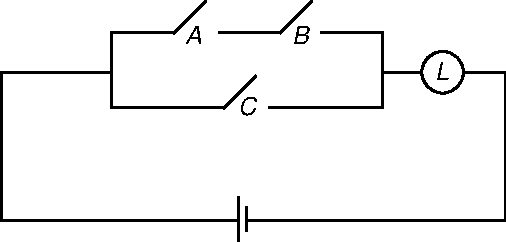
\includegraphics[scale=0.6]{img/circuito-pro-4}
 \]
si la probabilidad de estar cerrado el interruptor $A$ es $0.8$, el $B$ $0.9$ y el $C$ $0.7$, ¿cuál es la probabilidad
de que esté encendida la lámpara $L$?
}
%SOLUCIÓN
{}
%RESOLUCIÓN
{}


\newproblem{pro-5}{med}{}
%ENUNCIADO
{La probabilidad de contraer hepatitis a partir de una unidad de sangre es 0'01. Un paciente recibe dos unidades de
sangre durante su estancia en el hospital.
¿Cuál es la probabilidad de que contraiga hepatitis como consecuencia de ello?}
%SOLUCIÓN
{$0.0199$.}
%RESOLUCIÓN
{}


\newproblem*{pro-6}{far}{}
%ENUNCIADO
{En un lapso de tiempo una ameba puede morir con probabilidad 1/4 y dividirse en dos con probabilidad 1/2.
Durante el siguiente lapso de igual duración con cada ameba, independientemente de su origen, ocurre lo mismo.
¿Cuántas amebas y con qué probabilidad pueden existir al final del segundo intervalo de tiempo?
}
%SOLUCIÓN
{}
%RESOLUCIÓN
{}


\newproblem*{pro-7}{gen}{*}
%ENUNCIADO
{Supongamos los sucesos independientes $A_{1}$ y $A_{2}$ con probabilidades $p_{1}$ y $p_{2}$ respectivamente, e
incompatibles ambos con el suceso $A_{3}$ con probabilidad $p_{3}$ ($A_{1}$, $A_{2}$ y $A_{3}$ son sucesos de un mismo
espacio muestral).
Calcular en función de $p_{1}$, $p_{2}$ y $p_{3}$ las probabilidades de los siguientes sucesos:
\begin{enumerate}
\item  $A_{1}-(A_{2}\cup A_{3})$.
\item  $\overline{A_{1}\cup A_{2}\cup A_{3}}$.
\item  $A_{1}/(A_{2}\cup A_{3})$.
\end{enumerate}
}
%SOLUCIÓN
{}
%RESOLUCIÓN
{}


\newproblem{pro-8}{gen}{}
%ENUNCIADO
{Sean $A$ y $B$ sucesos de un mismo espacio muestral, tales que $P(A)=0.6$ y $P(A\cup B)=0.9$.
Calcular $P(B)$ si:
\begin{enumerate}
\item  $A$ y $B$ son independientes.
\item  $A$ y $B$ son incompatibles.
\end{enumerate}
}
%SOLUCIÓN
{
\begin{enumerate}
\item $P(B)=0.75$.
\item $P(B)=0.3$.
\end{enumerate}
}
%RESOLUCIÓN
{}


\newproblem{pro-9}{med}{*}
%ENUNCIADO
{En un estudio sobre el tabaco, se informa que el 40\% de los fumadores tiene un padre fumador, el 25\% tiene una madre
fumadora, y el 52\% tiene al menos uno de los dos padres fumadores. Se elige una persona fumadora al azar.
Calcular:
\begin{enumerate}
\item Probabilidad de que la madre sea fumadora si lo es el padre.
\item Probabilidad de que la madre sea fumadora si no lo es el padre.
\item ¿Son independientes el tener padre fumador y el tener madre fumadora?
\end{enumerate}
}
%SOLUCIÓN
{Llamando $PF$ al suceso que consiste en tener un padre fumador y $MF$ a tener una madre fumadora:
\begin{enumerate}
\item $P(MF/PF)=0.325$.
\item $P(MF/\overline{PF})=0.2$.
\item No son independientes.
\end{enumerate}
}
%RESOLUCIÓN
{Llamando $PF$ al suceso que consiste en tener un padre fumador y $MF$ a tener una madre fumadora, del enunciado se
tiene que $P(PF)=0.4$, $P(MF)=0.25$ y $P(PF\cup MF)=0.52$.
\begin{enumerate}
\item Nos piden la probabilidad de tener madre fumadora condicionada por tener padre fumador. Según la definción de
probabilidad condicionada se tiene
\[
P(MF/PF) = \frac{P(MF\cap PF)}{P(PF)}.
\]
A su vez, la probabilidad de la intersección de tener madre y padre fumadores puede calcularse a partir de la fórmula
de la unión:
\[
P(MF\cup PF) = P(MF)+P(PF)-P(MF\cap PF) \Leftrightarrow P(MF\cap PF) = P(MF)+P(PF)-P(MF\cup PF) = 0.4+0.25-0.52= 0.13,
\]
de modo que la probabilidad condicionada queda
\[
P(MF/PF) = \frac{P(MF\cap PF)}{P(PF)} = \frac{0.13}{0.4}=0.33.
\]
\item Ahora nos piden la probabilidad de tener madre fumadora condicionada por tener padre no fumador. De nuevo, según
la definición de probabilidad condicionada se tiene
\[
P(MF/\overline{PF}) = \frac{P(MF\cap \overline{PF})}{P(\overline{PF})}.
\]
Como el suceso $MF\cap \overline{PF}$ es la diferencias del suceso $MF$ y el suceso $PF$, su probabilidad se puede
calcular como
\[
P(MF\cap \overline{PF}) = P(MF)-P(MF\cap PF) = 0.25-0.13 = 0.12,
\]
de modo que la probabilidad condicionada queda
\[
P(MF/\overline{PF}) = \frac{P(MF\cap \overline{PF})}{P(\overline{PF})} = \frac{0.12}{1-0.4}=0.2.
\]
\item Como $P(MF)=0.25\neq 0.33=P(MF/PF)$ se puede concluir que los sucesos no son independientes. 
\end{enumerate}
}


\newproblem{pro-10}{med}{}
%ENUNCIADO
{El tétanos es mortal en el 70\% de los casos.
Si tres personas contraen el tétanos, ¿Cuál es la probabilidad de que mueran al menos dos de los tres?
}
%SOLUCIÓN
{$0.784$.}
%RESOLUCIÓN
{}


\newproblem{pro-11}{med}{*}
%ENUNCIADO
{Un equipo de atención primaria de salud realiza un estudio de la población, para evaluar la incidencia de hipertensión
e hipercolesterolemia.
Para ello analizan a 1000 personas de dicha población, seleccionadas aleatoriamente, encontrándose que 180 presentan
hipertensión, 140 hipercolesterolemia y 800 ninguna de ambas.
Se pide calcular la probabilidad de que una persona tomada al azar.
\begin{enumerate}
\item  Presente ambas enfermedades.
\item  Presente hipertensión si no presenta hipercolesterolemia.
\end{enumerate}
}
%SOLUCIÓN
{Llamando $HT$ a tener hipertensión y $HC$ a tener hipercolesterolemia:
\begin{enumerate}
\item $P(HT\cap HC)=0.12.$
\item $P(HT/\overline{HC})=0.0698.$
\end{enumerate} 
}
%RESOLUCIÓN
{}


\newproblem{pro-12}{gen}{*}
%ENUNCIADO
{Tras observar los resultados de la prueba de selectividad se sabe que el 40\% de los alumnos aprueba el examen de
Matemáticas, el 30\% el examen de Física y el 55\% suspenden los dos.
Si se elige un alumno al azar, calcular:
\begin{enumerate}
\item Probabilidad de que haya aprobado al menos uno de los dos exámenes.
\item Probabilidad de que haya aprobado Matemáticas si ha aprobado Física.
\item Probabilidad de que haya aprobado Física si ha suspendido Matemáticas.
\item ¿Son independientes aprobar Matemáticas y aprobar Física?
\end{enumerate}
}
%SOLUCIÓN
{Llamando $M$ al suceso correspondiente a aprobar Matemáticas y $F$ a aprobar Física:
\begin{enumerate}
\item $P(M\cup F)=0.45$.
\item $P(M/F)=0.83$.
\item $P(F/\overline{M})=0.08$.
\item No son independientes.
\end{enumerate}
}
%RESOLUCIÓN
{}


\newproblem{pro-13}{fis}{*}
%ENUNCIADO
{La probabilidad de que una lesión $A$ se reproduzca es $4/5$, la de que se reproduzca otra lesión $B$ es $1/2$, y la de que ambas se
reproduzcan $1/3$. Hallar la probabilidad de que:
\begin{enumerate}
\item Sólo se reproduzca la lesión $B$.
\item Al menos una se reproduzca.
\item Se reproduzca la lesión $B$ si se ha reproducido la $A$.
\item Se reproduzca la lesión $B$ si no se reproduce la lesión $A$.
\end{enumerate}
}
%SOLUCIÓN
{Llamando $A$ y $B$ a los sucesos consistentes en que se reproduzcan las respectivas lesiones, se tiene:
\begin{enumerate}
\item $P(B\cap\overline{A})=1/6$.
\item $P(A\cup B)=29/30$.
\item $P(B/A)=5/12$.
\item $P(B/\overline{A})=5/6$.
\end{enumerate}
}
%RESOLUCIÓN
{Llamemos $A$ y $B$ a los sucesos consistentes en que se reproduzcan las respectivas lesiones. Según el enunciado tenemos
$P(A)=4/5$, $P(B)=1/2$ y $P(A\cap B)=1/3$.

\begin{enumerate}
\item Para que sólo se reproduzca la lesión $B$ debe cumplirse el suceso $B-A$, es decir $B\cap\overline{A}$.
\[P(B\cap\overline{A})=P(B)-P(A\cap B)=1/2-1/3=1/6.\]

\item Para que se reproduzca al menos una lesión debe cumplirse el suceso $A\cup B$.
\[P(A\cup B)=P(A)+P(B)-P(A\cap B)=4/5+1/2-1/3=29/30.\]

\item El suceso consistente en que se reproduzca la lesión $B$ si se ha reproducido la $A$ es $B/A$.
\[P(B/A)=\frac{P(A\cap B)}{P(A)}=\frac{1/3}{4/5}=5/12.\]

\item El suceso consistente en que se reproduzca la lesión $B$ si no se ha reproducido la $A$ es $B/\overline{A}$.
\[P(B/\overline{A})=\frac{P(\overline{A}\cap B)}{P(\overline{A})}=\frac{1/6}{1-4/5}=5/6.\]
\end{enumerate}
}


\newproblem*{pro-14}{med}{}
%ENUNCIADO
{A partir de una investigación realizada, se sabe que el 10\% de las personas de 50 años sufren un tipo particular de
artritis.
Se ha desarrollado un procedimiento para detectar esta enfermedad, y por las pruebas realizadas se observa que si se
aplica el procedimiento a individuos que padecen la enfermedad, da positivo en el 85\% de los casos, mientras que
si se aplica a individuos sanos, da positivo en el 4\% de los casos.
Se pide:
\begin{enumerate}
\item  Calcular la probabilidad de que realizado el procedimiento a una persona, el resultado sea positivo.
\item  Si el resultado de aplicar el procedimiento a una persona ha sido positivo, ¿Cuál es la probabilidad de que
padezca la enfermedad?
\end{enumerate}
}
%SOLUCIÓN
{}
%RESOLUCIÓN
{}


\newproblem{pro-15}{gen}{*}
%ENUNCIADO
{En un experimento aleatorio se pueden dar dos sucesos $A$ y $B$, y se sabe que $P(B)=0.4$, $P(A/B)=0.3$ y
$P(A/\overline{B})=0.2$.
Calcular las siguientes probabilidades:
\begin{enumerate}
\item $P(A)$.
\item $P(\overline{A}\cap \overline{B})$.
\item $P(\overline{A}\cup \overline{B})$.
\end{enumerate}
}
%SOLUCIÓN
{
\begin{enumerate}
\item $P(A)=0.24$.
\item $P(\overline{A}\cap \overline{B})=0.52$.
\item $P(\overline{A}\cup \overline{B})=0.88$.
\end{enumerate}
}
%RESOLUCIÓN
{}


\newproblem{pro-16}{med}{*}
%ENUNCIADO
{En un servicio clínico digestivo se sabe que, de cada 1000 pacientes con dolor de estómago, 700 presentan gastritis,
200 presentan úlcera y 100 presentan cáncer.
En el análisis de la sintomatología gástrica, se ha comprobado que las probabilidades de presentar vómitos son $0.3$ en
el caso de gastritis, $0.6$ en el caso de úlcera y $0.9$ en el caso de cáncer.
Llega un nuevo paciente con dolor de estómago que, además, presenta vómitos.
¿Qué diagnosticaríamos?}
%SOLUCIÓN
{Llamando $G$ a tener gastritis, $U$ a tener úlcera, $C$ a tener cáncer y $V$ a tener vómitos, $P(G/V)=0.5$,
$P(U/V)=0.286$ y $P(C/V)=0.214$, de modo que se diagnosticaría gastritis.}
%RESOLUCIÓN
{}


\newproblem{pro-17}{gen}{*} 
%ENUNCIADO
{Un estudiante se somete a un examen de tipo test en el que cada pregunta tiene 3 respuestas posibles.
El estudiante se sabe el 40\% de las preguntas, y el resto las contesta al azar.
Se elige al azar una pregunta.
¿Qué probabilidad hay de que no la supiera si la contestó correctamente?
}
%SOLUCIÓN
{$1/3$.}
%RESOLUCIÓN
{}


\newproblem*{pro-18}{med}{*}
%ENUNCIADO
{Un test diseñado para diagnosticar el cáncer de cuello uterino da resultado positivo en el 10\% de los casos en los
que no existe la enfermedad, y da negativo en el 5\% de los casos en los que sí que existe la enfermedad.

Se sabe que en una cierta población de mujeres, el 4\% padece dicha enfermedad.
Si una mujer elegida aleatoriamente se somete al test, y da positivo, ¿qué probabilidad hay de que padezca la
enfermedad?}
%SOLUCIÓN
{}
%RESOLUCIÓN
{}


\newproblem{pro-19}{med}{*}
%ENUNCIADO
{Se ha desarrollado un nuevo test diagnóstico para detectar el síndrome de Down en niños recién nacidos, con un
sensibilidad del 80\% y una especificidad del 90\%.
Si en una determinada población en la que hay un 1\% de recién nacidos con el síndrome, al aplicarle el test a un niño,
da positivo, ¿cuál es la probabilidad de que tenga el síndrome?
¿le diagnosticarías la enfermedad?
¿Cuál debería ser la especificidad mínima del test para diagnosticar el síndrome en el caso de dar positivo?

Nota: La \emph{sensibilidad} de un test diagnóstico es la proporción de personas con la enfermedad que tienen un
resultado positivo en el test, mientras que la \emph{especificidad} del test es la proporción de personas sin la
enfermedad que tienen un resultado negativo en el test.}
%SOLUCIÓN
{Llamando $S$ a tener el síndrome de Down y $+$ a que el test de positivo, $P(S/+)=0.0748$ y
$P(\overline{S}/+)=0.9252$, de modo que no se diagnosticaría el síndrome al ser más probable que no lo tenga.\\
La especificidad mínima para que el test diagnostique el síndrome es $P(-/\overline{S})=0.9919$.}
%RESOLUCIÓN
{}


\newproblem{pro-20}{med}{*}
%ENUNCIADO
{En un estudio se han probado tres tipos de tratamientos $A$, $B$ y $C$ contra una determinada enfermedad. De los
pacientes participantes en el estudio, el 50\% fueron tratados con el tratamiento $A$, el 30\% con el $B$ y el 20\% con
el $C$.
Posteriormente se observaron los pacientes que sanaron y los que tuvieron algún efecto secundario, según se
muestra en la siguiente tabla:
\[
\begin{array}{|c|c|c|c|}
\hline
\text{Tratamiento} & \text{Sanados} & \text{Con efectos secundarios} \\
\hline
A & 86\% & 12\% \\
\hline
B & 92\% & 14\% \\
\hline
C & 81\% &  6\% \\
\hline
\end{array}
\]
Se pide:
\begin{enumerate}
\item Si se selecciona un enfermo al azar, ¿cuál es la probabilidad de que haya sanado?
¿Y de que haya tenido algún efecto secundario? 
\item Si un enfermo ha sanado, ¿qué tratamiento es más probable que haya recibido?
¿Y si en vez de decirnos que ha sanado nos dicen que no ha tenido efectos secundarios?
\item Si en total hay un 8\% pacientes que no sanaron pero que tampoco tuvieron efectos secundarios, ¿cuál es la
probabilidad de que un enfermo se haya curado sin tener efectos secundarios?
\end{enumerate}
}
%SOLUCIÓN
{Llamado $S$ a sanar y $E$ a tener efectos secundarios:
\begin{enumerate}
\item $P(S)=0.868$ y $P(E)=0.114$.
\item $P(A/S)=0.495$, $P(B/S)=0.318$ y $P(C/S)=0.187$.\\
$P(A/\overline{E})=0.497$, $P(B/\overline{E})=0.291$ y $P(C/\overline{E})=0.212$.\\
En ambos casos el tratamiento más probable es el $A$.
\item $P(S\cap \overline{E})=0.806$.
\end{enumerate}
}
%RESOLUCIÓN
{}


\newproblem*{pro-21}{nut}{}
%ENUNCIADO
{En una plantación hay tres variedades de uvas A,B y C en un 45\%, 35\% y 20\% respectivamente. Se sabe que el porcentaje de vides infectadas por una bacteria es del 5\% en la variedad A, del 12\% en la variedad B y del 18\% en la C. Si se toman uvas de una vid elegida al azar, ¿cuál es la probabilidad de que estén infectadas? Si las uvas cogidas de una vid están infectadas, ¿de qué variedad es más probable que sean?
}
%SOLUCIÓN
{}
%RESOLUCIÓN
{}


\newproblem*{pro-22}{amb}{}
%ENUNCIADO
{Se sabe que el 25\% de las plantas afectadas por un vertido tóxico están contaminadas. Se ha
desarrollado un procedimiento para detectar la contaminación, y por las
pruebas realizadas se observa que si se aplica el procedimiento a plantas contaminadas, da positivo en el 96\% de los casos, mientras que
si se aplica plantas no contaminadas, da positivo en el 8\% de los casos. Se pide:

\begin{enumerate}
\item  Calcular la probabilidad de que al aplicar el procedimiento a una planta elegida al azar, el resultado sea positivo.

\item  Si el resultado de aplicar el procedimiento a una planta ha sido
positivo, ¿Cuál es la probabilidad de que esté contaminada?
\end{enumerate}
}
%SOLUCIÓN
{}
%RESOLUCIÓN
{}


\newproblem*{pro-23}{amb}{}
%ENUNCIADO
{Un test para detectar la contaminación del agua tiene una sensibilidad del $97.5$\% y una especificidad del 95\%. Se pide:
\begin{enumerate}
\item ¿Qué relación existe entre la probabilidad de que el agua esté contaminada y la de que el test de positivo?
\item Si se aplica el test a muestras de 20 embalses y resulta positivo en 5 de las muestras, según la relación anterior, ¿qué porcentaje de embalses se estima que están contaminados?
\item Suponiendo que el porcentaje real de embalses contaminados es del 12\%, ¿cuál es la probabilidad de que un embalse esté contaminado si el resultado del test es negativo?
\end{enumerate}
}
%SOLUCIÓN
{}
%RESOLUCIÓN
{}


\newproblem*{pro-24}{med}{*}
% ENUNCIADO
{El dolor intenso sin derrame en una zona concreta de la articulación de la rodilla es síntoma de esguince en el Ligamento Lateral Externo
de la misma (L.L.E.). Si los esguinces en dicho ligamento se clasifican como: de grado 1, cuando hay simple distensión, que se presenta en
un 60\% de los casos; de grado 2, cuando hay ruptura parcial, que se presenta en un 30\% de los casos; y de grado 3, cuando hay ruptura
total, que se presenta en un 10\%. Y teniendo en cuenta que el síntoma se presenta en un 80\% de los que tienen el esguince de grado 1, en
un 90\% de los de grado 2, y en un 100\% de los de grado 3:
\begin{enumerate}
\item Si una persona se produce un esguince de L.L.E., ¿cuál es la probabilidad total de que padezca dolor intenso sin
derrame?
\item Si una persona llega a una consulta con dolor intenso sin derrame en la zona adecuada de la rodilla, ¿cuál sería
el diagnóstico?
\item De un total de 10000 personas analizadas con dolor intenso sin derrame en la zona adecuada de la rodilla,
¿cuántas se espera que hayan sufrido un esguince de grado 1?
¿Y de grado 2?
¿Y de grado3?
\item Si mantenemos iguales el resto de probabilidades dadas como dato, ¿cuáles deben ser las probabilidades de
esguince de grado 2 y de grado 3 para que la probabilidad de esguince de grado 2 si se padece el síntoma sea igual a la
de grado 3 si se padece el síntoma?
\end{enumerate}
}
%SOLUCIÓN
{}
%RESOLUCIÓN
{}


\newproblem{pro-25}{med}{*}
%ENUNCIADO
{En una población se ha vacunado a la tercera parte de los individuos contra la gripe.
Trascurrido el invierno, se comprueba que la probabilidad de estar vacunado si se tiene la gripe es $0.2$, y que el
10\% de los vacunados tuvieron gripe.
\begin{enumerate}
\item ¿Cuál fue la incidencia de la epidemia de gripe?\\
(Nota: La incidencia de una epidemia es la probabilidad de
personas infectadas).
\item ¿Cuál es la probabilidad de que una persona no vacunada contraiga la gripe?
\item ¿Se puede afirmar que la vacuna tiene alguna eficacia?
\end{enumerate}
}
%SOLUCIÓN
{Llamando $G$ al suceso consistente en tener la gripe y $V$ a estar vacunado:
\begin{enumerate}
\item $P(G)=1/6$.
\item $P(G/\overline{V})=0.2$.
\item Si resulta eficaz, aunque poco.
\end{enumerate}
}
%RESOLUCIÓN
{}


\newproblem*{pro-26}{amb}{*}
%ENUNCIADO
{Una zona de un Parque Nacional se ha repoblado con 10000
árboles, de los cuales 5000 han sido pinos, 4000 encinas y 1000
fresnos. Al cabo de un año se hace recuento y se observa que han
sobrevivido 4500 pinos, 2000 encinas y 900 fresnos. Suponiendo que
los resultados obtenidos son aplicables a una nueva zona del Parque
Nacional que se va a repoblar:
\begin{enumerate}
\item ¿Cuál es la probabilidad de que un árbol que se va a plantar
muera durante el primer año?
\item ¿Cuál es la probabilidad de que muera y sea pino?
\item Si sabemos que el árbol ha vivido, ¿cuál es la probabilidad de
que sea un fresno?
\item Si sabemos que el árbol ha muerto, ¿cuál es la probabilidad de
que sea una encina?
\end{enumerate}
}
%SOLUCIÓN
{}
%RESOLUCIÓN
{}


\newproblem*{pro-27}{gen}{}
%ENUNCIADO
{Sean $A$, $B$ y $C$ sucesos arbitrarios de un experimento
aleatorio. Se consideran los siguientes sucesos:
\begin{quote}
    $E_1$=\{al menos dos de los sucesos ocurren\},\\
    $E_2$=\{exactamente dos de los sucesos ocurren\},\\
    $E_3$=\{al menos uno de los sucesos ocurre\},\\
    $E_4$=\{exactamente uno de los sucesos ocurre\},\\
    $E_5$=\{no m\'{a}s de dos sucesos ocurren\}.
\end{quote}
Expresar $E_1$, $E_2$, $E_3$, $E_4$ y $E_5$ en función de $A$,$B$ y $C$.
}
%SOLUCIÓN
{}
%RESOLUCIÓN
{}


\newproblem*{pro-28}{gen}{}
%ENUNCIADO
{La probabilidad de que un hombre siga vivo dentro de 25 años es 3/5, y la de que su esposa lo esté es 2/3. Si
ambos sucesos son independientes, hallar la probabilidad de que en ese momento:
\begin{enumerate}
\item Ambos estén vivos.
\item Sólo el hombre viva.
\item Sólo viva la esposa.
\item Al menos uno esté vivo.
\item Viva el hombre si vive la esposa.
\item Viva el hombre si no vive la esposa.
\end{enumerate}
}
%SOLUCIÓN
{}
%RESOLUCIÓN
{}


\newproblem*{pro-29}{gen}{}
%ENUNCIADO
{La probabilidad de que un hombre siga vivo dentro de 25 años es 3/5, la de que su esposa lo esté es 2/3 y la de que
ambos vivan es 1/2. Hallar la probabilidad de que en ese momento:
\begin{enumerate}
\item Sólo el hombre viva.
\item Sólo viva la esposa.
\item Al menos uno esté vivo.
\item Viva el hombre si vive la esposa.
\item Viva el hombre si no vive la esposa.
\end{enumerate}
}
%SOLUCIÓN
{}
%RESOLUCIÓN
{}


\newproblem*{pro-30}{gen}{}
%ENUNCIADO
{El 40\% de los alumnos que han suspendido matemáticas deciden preparar el examen extraordinario en una academia, el
35\% decide asistir a las clases que organiza la propia universidad y el resto lo prepara por su cuenta.
De experiencias previas, se sabe que el 30\% de los alumnos de academia consigue aprobar el examen, de los alumnos que
asisten a la universidad aprueban el 45\%, y del resto de los alumnos aprueban el 25\%.
Se pide:
\begin{enumerate}
\item ¿Cuál es la probabilidad de que un alumno elegido al azar apruebe el examen?
\item Si un alumno ha suspendido, ¿cuál es la probabilidad de que haya asistido a una academia?
\end{enumerate}
}
%SOLUCIÓN
{}
%RESOLUCIÓN
{}


\newproblem*{pro-31}{gen}{}
%ENUNCIADO
{Se dispone de dos urnas, la primera con 10 bolas blancas y 6 bolas negras, y la segunda con 5 bolas rojas, 8 bolas
azules y 3 bolas verdes.
Construir el espacio muestral del experimento que consiste en sacar una bola de cada urna, y
del experimento que consistiría en sacar dos bolas de cada urna.}
%SOLUCIÓN
{}
%RESOLUCIÓN
{}


\newproblem*{pro-32}{amb}{}
%ENUNCIADO
{Una ciudad se abastece de agua de tres pantanos: $A$ en un 50\%, $B$ en un 40\% y $C$ en un 10\%. El agua del pantano $A$ produce diarrea en un 3\% de los casos, la del $B$ en un 1\% y la del $C$ en un $7\%$. ¿Cual es la probabilidad de que una persona que beba agua en la ciudad tenga diarrea? Si una persona presenta diarrea por causa del agua, ¿de qué pantano es más probable que provenga dicha agua?
}
%SOLUCIÓN
{}
%RESOLUCIÓN
{}

\newproblem*{pro-33}{gen}{}
%ENUNCIADO
{Construir el espacio muestral de los siguientes experimentos aleatorios:
\begin{enumerate}
\item Seleccionar una persona al azar y medir su sexo y si es fumadora o no. 
\item Seleccionar una persona al azar y medir su grupo sanguíneo y si es fumadora o no.
\item Seleccionar una persona al azar y medir su sexo, grupo sanguíneo y se es fumadora o no.
\end{enumerate}
}
%SOLUCIÓN
{}
%RESOLUCIÓN
{}


\newproblem*{pro-34}{amb}{*}
%ENUNCIADO
{Un test diagnóstico permite detectar la presencia de un tóxico en el pescado con una sensibilidad del 96\% y una especificidad del 92\%. Si un vertido ha afectado a las tres quintas partes del pescado de un lago, se pide:
\begin{enumerate}
\item ¿Cuál es la probabilidad de que al aplicar el test a un pescado  elegido al azar de negativo?
\item Si el test da negativo en un pescado, ¿es más probable que esté contaminado o que no lo esté?
\item ¿Podríamos decir lo mismo en un lago donde el 90\% de los pescados hayan sido contaminados?
\end{enumerate}
}
%SOLUCIÓN
{}
%RESOLUCIÓN
{}


\newproblem*{pro-35}{amb}{}
%ENUNCIADO
{Se han realizado tres campañas $A$, $B$ y $C$ de sensibilización para el reciclaje de vidrio y papel. La campaña $A$ se ha aplicado al 50\% de la población, la $B$ al 20\%, y al resto se la ha aplicado la $C$. Posteriormente se observaron las personas que acabaron reciclando habitualmente el vidrio y el papel, obteniendo los siguientes resultados
\begin{center}
\begin{tabular}{|c|c|c|}
\hline
$A$ & 56\% & 42\% \\
\hline
$B$ & 52\% & 46\% \\
\hline
$C$ & 71\% & 38\% \\
\hline
\end{tabular}
\end{center}
Se pide:
\begin{enumerate}
\item Si se selecciona un individuo al azar, ¿cuál es la probabilidad de que recicle vidrio? ¿Y de que recicle papel?
\item Si un individuo recicla vidrio, ¿qué campaña es más probable que haya recibido? ¿Y si en vez de decirnos que recicla vidrio nos dicen que recicla papel?
\item Si en total hay un 18\% de personas que no reciclan ni vidrio ni papel, ¿cuál es la probabilidad de que una persona recicle vidrio si no recicla papel?
\end{enumerate}
}
%SOLUCIÓN
{}
%RESOLUCIÓN
{}


\newproblem*{pro-36}{far}{*}
%ENUNCIADO
{Una enfermedad se trata con 3 fármacos diferentes, $A$, $B$ y $C$. El fármaco $A$ se aplica a un 30\% de los hombres y a un 50\% de las mujeres; el fármaco $B$ se aplica a un 60\% de los hombres y a un 20\% de las mujeres; y el fármaco $C$ a un 10\% de los hombres y al 30\% de las mujeres. Además, se sabe que del total de afectados por la enfermedad el 40\% son hombres y el 60\% mujeres.

Teniendo en cuenta que cada persona enferma es tratada únicamente con un fármaco, se pide:
\begin{enumerate}
\item Si tenemos un paciente con esa enfermedad, ¿cuál es el fármaco que con más probabilidad se le aplicaría?
\item Si tenemos un paciente tratado con $B$, ¿cuál es la probabilidad de que sea hombre?
\item Si tenemos un paciente que no ha sido tratado con $C$, ¿cuál es la probabilidad de que se mujer?
\end{enumerate}
}
%SOLUCIÓN
{}
%RESOLUCIÓN
{}


\newproblem{pro-37}{far}{*}
%ENUNCIADO
{Una enfermedad se trata con 3 medicamentos diferentes: A en un 50\% de los casos, B en un 30\% y C en un 20\%, todo
ello independientemente de si se es hombre o mujer.
Si sabemos que el medicamento A produce efectos secundarios en un 5\% de los hombres y en un 10\% de las mujeres, el B
en un 15\% de los hombres y en un 5\% de las mujeres, y el C en un 8\% de los hombres y en un 13\% de las mujeres, se pide:
\begin{enumerate}
\item ¿En qué colectivo resulta más probable que haya efectos secundarios, en hombres o en mujeres?
Justificar adecuadamente la respuesta.
\item Calcular la probabilidad de que un hombre que presenta efectos secundarios haya sido tratado con C, y la de que
una mujer que no los presenta haya sido tratada con A.
\item Si en total de enfermos hay un 65\% de hombres y un 35\% de mujeres, ¿qué probabilidad hay de que un enfermo que
no presenta efectos secundarios sea mujer?
\end{enumerate}
}
%SOLUCIÓN
{Llamando $EH$ a que un hombre tenga efectos secundarios y $EM$ a que los tenga una mujer:
\begin{enumerate}
\item $P(EH)=0.086$ y $P(EM)=0.091$.
\item $P(C/EH)=0.186,$ y $P(A/\overline{EM})=0.495$.
\item $P(M/\overline E )= 0.349$.
\end{enumerate}
}
%RESOLUCIÓN
{Según el enunciado, si llamamos $A$ al suceso haber sido tratado con el medicamento A, y de forma similar a los sucesos $B$ y $C$, entonces sus respectivas probabilidades son: $P(A)=0.5$, $P(B)=0.3$ y $P(C)=0.2$, y todo ello tanto para hombres como para mujeres.

Además, también se nos dan como datos las sucesivas probabilidades condicionadas de que se produzcan efectos secundarios al tomar cada uno de los fármacos, tanto en hombres como en mujeres. Si llamamos $EH$ al suceso efectos secundarios en hombres y $EM$ al suceso efectos secundarios en mujeres, entonces los datos del problema son: $P(EH/A)=0.05$, $P(EM/A)=0.10$, $P(EH/B)=0.15$, $P(EM/B)=0.05$, $P(EH/C)=0.08$, y $P(EM/C)=0.13$. De lo anterior pueden deducirse fácilmente las probabilidades de sus complementarios: $P(\overline{EH}/A)=0.95$, $P(\overline{EM}/A)=0.90$, $P(\overline{EH}/B)=0.85$, $P(\overline{EM}/B)=0.95$, $P(\overline{EH}/C)=0.92$, y $P(\overline{EM}/C)=0.87$.
\begin{enumerate}
\item Teniendo en cuenta las probabilidades anteriores y aplicando el teorema de probabilidad total:
\begin{align*}
P(EH) &=P(A)P(EH/A)+P(B)P(EH/B)+P(C)P(EH/C)=\\
&=0.5\cdot0.05+0.3\cdot0.15+0.2\cdot0.08=0.086,\\
P(EM) &=P(A)P(EM/A)+P(B)P(EM/B)+P(C)P(EM/C)=\\
&=0.5\cdot0.1+0.3\cdot0.05+0.2\cdot0.13=0.091.
\end{align*}
Por lo tanto, resulta más probable que sean las mujeres las que tengan efectos secundarios.

\item Según el teorema de Bayes, la probabilidad de que un hombre que presenta efectos secundarios haya sido tratado con C es:
\[
P(C/EH) = \frac{{P(C)P(EH/C)}}{{P(EH)}} = \frac{{0.2 \cdot 0.08}}{{0.086}} = 0.186.
\]

De manera muy parecida, la probabilidad de que una mujer que no presenta efectos secundarios haya sido tratada con A vale:
\[
P(A/\overline {EM} ) = \frac{{P(A)P(\overline {EM} /A)}}{{P(\overline {EM} )}} = \frac{{0.5 \cdot 0.9}}{{1 - 0.091}} = 0.495.
\]

\item Si en el total de enfermos hay un 65\% de hombres ($P(H)=0.65$) y un 35\% de mujeres ($P(M)=0.35$), y teniendo en cuenta que ya hemos calculado en el primer apartado las probabilidades de padecer efectos secundarios si se es hombre ($P(EH)=0.086$) y de efectos secundarios si se es mujer ($P(EM)=0.091$), aplicando el teorema de Bayes:
\[
P(M/\overline E ) = \frac{{P(M)P(\overline {EM} )}}{{P(H)P(\overline {EH} ) + P(M)P(\overline {EM} )}} = \frac{{0.35 \cdot 0.909}}{{0.65 \cdot 0.914 + 0.35 \cdot 0.909}} = 0.349.
\]
\end{enumerate}
}


\newproblem{pro-38}{gen}{}
%ENUNCIADO
{Se sabe que los grupos sanguíneos en una determinada población se distribuyen con las siguientes frecuencias:
\[
0: 30\% \quad A:45\% \quad B: 18\% \quad AB:7\% 
\]
Por otro lado, también se sabe que la octava parte de los individuos del grupo $0$ tienen RH negativo, así como la
cuarta parte del grupo $A$, la mitad del grupo $B$, y la tercera parte del grupo $AB$.

Se pide:
\begin{enumerate}
\item ¿Cuál es la probabilidad de que un indiviudo elegido al azar sea del tipo $A$ y tenga RH positivo?
\item ¿Cuál es la probabilidad de que un individuo elegido al azar tenga RH negativo o sea del grupo universal?
\item Si un individuo elegido al azar tiene RH positivo, ¿cuál es la probabilidad de que pertenezca al grupo $B$?
\end{enumerate} 
}
%SOLUCIÓN
{Llamando $0$ a tener grupo 0, $A$ a tener grupo $A$, $B$ a tener grupo $B$, $AB$ a tener grupo $AB$, $+$ a tener RH
positivo y $-$ a tener RH negativo:
\begin{enumerate}
\item $P(A\cap +)=0.34.$
\item $P(-\cup 0)=0.53.$
\item $P(B/+)=0.12$.
\end{enumerate}
}
%RESOLUCIÓN
{Llamando $0$ a tener grupo 0, $A$ a tener grupo $A$, $B$ a tener grupo $B$, $AB$ a tener grupo $AB$, $+$ a tener RH
positivo y $-$ a tener RH negativo, del enunciado se tiene:
\[
\begin{array}{lllll}
P(0)=0.3 & \quad & P(-/0)= 1/8 & \quad & P(+/0)=1-1/8=7/8,\\
P(A)=0.45 & & P(-/A)=1/4 & & P(+/A)=1-1/4=3/4,\\
P(B)=0.18 & & P(-/B)=1/2 & & P(+/B)=1-1/2=1/2,\\
P(AB)=0.07 & & P(-/AB)=1/3 & & P(+/AB)=1-1/3 = 2/3.
\end{array}
\]
\begin{enumerate}
\item La probabilidad que nos piden es la de la intersección del suceso $A$ y el suceso $+$, que vale
\[
P(A\cap +)=P(A)P(+/A)=0.45\frac{3}{4} = 0.34.
\]
\item La probabilidad que nos piden es la de la unión del suceso $-$ con el suceso $0$, que vale
\[
P(-\cup 0) = P(-)+P(0)-P(-\cap 0).
\]
A su vez, para calcular la probabilidad de tener RH negativo podemos utilizar el teorema de la probabilidad total,
partiendo de que los grupos sanguíneos forman un sistema completo de suceso, de manera que
\[
P(-) = P(0)P(-/0)+P(A)P(-/A)+P(B)P(-/B)+P(AB)P(-/AB) = 0.3\frac{1}{8}+0.45\frac{1}{4}+0.18\frac{1}{2}+0.07\frac{1}{3} =
0.26.
\]
Por otro lado, 
\[
P(-\cap 0) = P(0)P(-/0)=0.3\frac{1}{8}=0.04.
\]
Así que, finalmente la probabilidad que nos piden es
\[
P(-\cup 0) = P(-)+P(0)-P(-\cap 0) = 0.26 + 0.3 - 0.04 = 0.53.
\]
\item Ahora nos piden la probabilidad del suceso $B$ condicionado por el suceso $+$, que puede calcularse utilizando el
teorema de Bayes:
\[
P(B/+) = \frac{P(B)P(+/B)}{P(+)} = \frac{P(B)P(+/B)}{1-P(-)} = \frac{0.18\cdot 0.5}{1-0.26} = 0.12.
\]
\end{enumerate}
}


\newproblem{pro-39}{psi}{}
%ENUNCIADO
{Sabemos que el test de Bender para detectar alteraciones cerebrales tiene una sensibilidad del 88\% y una
especificidad del 96\%. 
Por otro lado, sabemos que en una población la probabilidad de que un individuo elegido al azar tenga alteraciones
cerebrales y además de positivo en el test es $0.08$.
Se pide: 
\begin{enumerate}
\item Calcular el porcentaje de personas que tienen alteraciones cerebrales en la población.
\item ¿Es efectivo el test en esta población para detectar la ausencia de alteraciones cerebrales?
\end{enumerate}
}
%SOLUCIÓN
{Llamando $E$ a presentar alteraciones cerebrales y $+$ y $-$ a que el test de positivo y negativo respectivamente:
\begin{enumerate}
\item $P(E)=0.0901$, es decir, un $9.09\%$.
\item $P(\overline{E}/-)= 0.99$, lo cual indica que es muy efectivo para detectar la ausencia de alteraciones
cerebrales.
\end{enumerate}
 }
%RESOLUCIÓN
{}


\newproblem{pro-40}{psi}{}
%ENUNCIADO
{Los estudios epidemiológicos indican que el 20\% de las personas mayores sufren un deterioro neuropsicológico.
También se sabe que la tomografía axial computerizada (TAC) puede detectar ese trastorno en el 90\% de los que lo
padecen, pero que también puede diagnosticarlo en el 5\% de las personas que no lo tienen.
Si se toma una persona al azar y el TAC da positivo, ¿cuál es la probabilidad de que realmente esté enfermo? } 
%SOLUCIÓN
{Llamando $E$ a sufrir el deterioro neuropsicológico y $+$ a que el TAC de positivo: $P(E/+)=0,82$.
}
%RESOLUCIÓN
{La tomografía axial computerizada es un test diagnostico que se utiliza para detectar el deterioro neuropsicológico,
así que, si llamamos $E$ a sufrir el deterioro neuropsicológico, entonces $P(E)=0.2$ ya que el 20\% de la población
tienen esta enfermedad, y si llamamos $+$ al que el TAC de positivo, entonces $P(+/E)=0.9$ pues el test detecta la
enfermedad en el 90\% de los pacientes enfermos, y $P(+/\overline{E})=0.05$ pues el test también la diagnostica en el
5\% de los pacientes sin esta enfermedad.

Para saber cuál es la probabilidad de que una persona en la que el test da positivo tenga la enfermedad, necesitamos
calcular la probabilidad de estar enfermo, condicionado por que el test de positivo, y para calcularla podemos utilizar
el teorema de Bayes, ya que $E$ y $\overline{E}$ forman un sistema completo de sucesos:
\[
P(E/+) = \frac{P(E)P(+/E)}{P(+)} = \frac{P(E)P(+/E)}{P(E)P(+/E)+P(\overline{E})P(+/\overline{E})} = \frac{0.2\cdot
0.9}{0.2\cdot 0.9+0.8\cdot 0.05} = 0.82.
\]
}


\newproblem{pro-41}{fis}{*}
%ENUNCIADO
{Un fisioterapeuta dispone de dos técnicas $A$ y $B$ para rehabilitar una determinada lesión. Se sabe que dicha lesión es 3 veces más
frecuentes en personas mayores de 30 años que en personas jóvenes. También se sabe que en las personas jóvenes, la técnica $A$ es efectiva
en el 30\% de los casos y la técnica $B$ en el 60\%, mientras que en personas mayores, la técnica $A$ es efectiva en el 50\% de los casos y
la técnica $B$ en el 70\%. Si, independiente de la edad, aplica la técnica $A$ el mismo número de veces que la técnica $B$, se pide:
\begin{enumerate}
\item ¿Cual es la probabilidad de que una persona joven elegida al azar se cure? ¿y la de que se cure una persona mayor?
\item ¿Cuál es la probabilidad de que una persona cualquiera se cure?
\item Si una persona mayor no se ha curado, ¿cuál es la probabilidad de que fuese tratado con la técnica $A$?
\end{enumerate}
} 
%SOLUCIÓN
{Llamemos $J$ al suceso consitente en que una persona con la lesión sea joven, $C$ al suceso consistente en curarse, y $A$ y $B$ a los sucesos consistentes en aplicar las respectivas técnicas de
rehabilitación:
\begin{enumerate}
\item $P(C/J)=0.45.$ y $P(C/\overline{J})=0.6$.
\item $P(C)=0.5625$.
\item $P(A/\overline{J}\cap \overline{C})=0.625$.
\end{enumerate}
}
%RESOLUCIÓN
{Llamemos $J$ al suceso consitente en que una persona con la lesión sea joven. Según el enunciado $P(\overline{J})=3P(J)$. Como además, se
cumple que $P(J)+P(\overline{J})=1$, tenemos que $P(J)+3P(J)=4P(J)=1$, con lo que $P(J)=1/4=0.25$ y $P(\overline{J})=0.75$.

Por otro lado, llamemos $C$ al suceso consistente en curarse, y $A$ y $B$ a los sucesos consistentes en aplicar las respectivas técnicas de
rehabilitación. Según el enunciado, la técnica $A$ cura al 30\% de los jóvenes con lesión, lo que, traducido a probabilidad, puede
escribirse como $P(C/J\cap A)=0.3$. Del mismo modo, del resto del enunciado se deduce $P(C/J\cap B)=0.6$, $P(C/\overline{J}\cap A)=0.5$ y
$P(C/\overline{J}\cap B)=0.7$.

Con estos datos, pasamos a contestar a las preguntas.
\begin{enumerate}
\item El suceso consistente en que una persona joven se cure puede expresarse como $C/J$. Para calcular su probabilidad podemos utilizar el
teorema de la probabilidad total aprovechando que $A/J$ y $B/J$ forma un sistema completo de sucesos.
\[
P(C/J)=P(A/J)P(C/J\cap A)+P(B/J)P(C/J\cap B).
\]
Como ambas técnicas se aplican el mismo número de veces independientemente de la edad, tenemos que $P(A/J)=0.5$ y $P(B/J)=0.5$, y por tanto,
\[
P(C/J)=0.5\cdot 0.3+0.5\cdot 0.6=0.45.
\]

Del mismo modo, la probabilidad de que se cure una persona mayor es
\[
P(C/\overline{J})=P(A/\overline{J})P(C/\overline{J}\cap A)+P(B/\overline{J})P(C/\overline{J}\cap B)=0.5\cdot 0.5+0.5\cdot 0.7=0.6.
\]

\item De nuevo, para calcular la probabilidad de que una persona lesionada se cure, podemos utilizar el teorema de la probabilidad total,
aprovechando que $J$ y $\overline{J}$ también forman un sistema completo de sucesos. Así, tenemos 
\[
P(C)= P(J)P(C/J)+P(\overline{J})P(C/\overline{J})= 0.25\cdot 0.45+0.75\cdot 0.6=0.5625.
\]

\item Por último, para calcular la probabilidad de que una persona mayor fuese tratada con la técnica $A$ si se ha curado, podemos utilizar
el teorema de Bayes:
\[
P(A/\overline{J}\cap \overline{C})=\frac{P(A/\overline{J})P(\overline{C}/\overline{J}\cap A)}{P(\overline{C}/\overline{J})}=
\frac{P(A/\overline{J})(1-P(C/\overline{J}\cap A))}{1-P(C/\overline{J})}=\frac{0.5\cdot(1-0.5)}{1-0.6}= 0.625.
\]
\end{enumerate}
}


\newproblem{pro-42}{med}{*}
%ENUNCIADO
{Para comprobar la eficacia de un test diagnóstico se lleva a cabo una experiencia cuyos resultados se recogen en la siguiente tabla:
\begin{center}
\begin{tabular}{|l|r|r|}
\cline{2-3}
\multicolumn{1}{l|}{} & Test $+$ & Test $-$ \\
\hline
Enfermos & 4680 & 120 \\
\hline
No Enfermos & 80 & 2020 \\
\hline
\end{tabular}
\end{center}
Calcular para dicho test:
\begin{enumerate}
\item Las probabilidades de verdadero negativo, verdadero positivo, falso negativo y falso positivo.
\item Los valores predictivos, tanto el positivo como el negativo.
\item La probabilidad de diagnóstico acertado.
\end{enumerate}
} 
%SOLUCIÓN
{
}
%RESOLUCIÓN
{
}


\newproblem{pro-43}{med}{*}
%ENUNCIADO
{Para diagnosticar una misma enfermedad se utilizan dos test $A$ y $B$ completamente independientes. Si la prevalencia de la enfermedad en
una población es de un 2\%, la sensibilidad de $A$ es de un 95\%, la sensibilidad de $B$ es de un 97\%, la especificidad de $A$ es de un
90\%, y la de $B$ de un 85\%, calcular:
\begin{enumerate}
\item El valor predictivo positivo del test $A$.
\item La probabilidad de que, aplicados ambos a un individuo cualquiera de la población, alguno de los test dé positivo.
\item La probabilidad de que, aplicados ambos a un individuo cualquiera de la población, los dos den diagnóstico erróneo.
\end{enumerate}
} 
%SOLUCIÓN
{
}
%RESOLUCIÓN
{
}


\newproblem{pro-44}{med}{*}
%ENUNCIADO
{Al aplicar un test diagnóstico a una población se obtuvieron un 1\% de personas enfermas en las que el test dio negativo, un 2\% de
personas sanas en las que el test dio positivo, y un 90\% de personas sanas en las que el test dio negativo.  
Se pide:
\begin{enumerate}
\item Calcular la prevalencia de la enfermedad.
\item Calcular la sensibilidad del test.
\item Calcular la especificidad del test.
\end{enumerate} 
} 
%SOLUCIÓN
{\begin{enumerate}
\item $P(E)=0.08$.
\item $P(+/E) = 0.875$.
\item $P(-/\overline{E})= 0.9783$.
\end{enumerate}
}
%RESOLUCIÓN
{El espacio muestral del experimento correspondiente a la aplicación del test diagnóstico aparece en el siguiente árbol
% \begin{center}
% \psset{treesep=0.6cm, levelsep=2.5cm, tpos=0.6}
% \renewcommand{\psedge}[2]{\ncdiag[armA=0.8cm,angleA=180,angleB=0,armB=0cm]{#2}{#1}} 
% \pstree[treemode=R, nodesep=1pt]{\Tp*}{
% 	\pstree[linestyle=none]{\TR[edge=none]{Enfermedad}}{
% 		\pstree{\TR{Test}}{
% 			\pstree{\TR{$E$}}{\TR{$P$}}
% 		}
% 	}
% 	\pstree{\TR{$E$}\taput{\scriptsize $P(E)$}}{
% 		\pstree[linestyle=none]{\TR{$+$}\taput{\scriptsize $P(+/E)$}}{
% 			\pstree{\TR{$(E,+)$}}{\TR{?}}
% 		}
% 		\pstree[linestyle=none]{\TR{$-$}\taput{\scriptsize $P(-/E)$}}{
% 			\pstree{\TR{$(E,-)$}}{\TR{$0.01$}}
% 		}
% 	}
% 	\pstree{\TR{$\overline E$}\taput{\scriptsize $P(\overline E)$}}{
% 		\pstree[linestyle=none]{\TR{$+$}\taput{\scriptsize $P(+/\overline E)$}}{
% 			\pstree{\TR{$(\overline E,+)$}}{\TR{$0.02$}}
% 		}
% 		\pstree[linestyle=none]{\TR{$-$}\taput{\scriptsize $P(-/\overline E)$}}{
% 			\pstree{\TR{$(\overline E,-)$}}{\TR{$0.9$}}
% 		}
% 	}
% 	\pstree[linestyle=none]{\Tp[edge=none]}{\Tp}
% }
% \end{center}

Como la probabilidad el espacio muestral es 1, se puede deducir que la probabilidad que falta $P(E,+))= 1- 0.01 -0.02 -0.9 = 0.07$.

\begin{enumerate}
\item La prevalencia de la enfermedad es 
\[
P(E) = P(E,+)+P(E,-) = 0.07 + 0.01 = 0.08,
\]
es decir, un 8\% de las personas de la población tienen la enfermedad.

\item La sensibilidad el test es
\[
P(+/E) = \frac{P(E\cap +)}{P(E)} = \frac{0.07}{0.08} = 0.875.
\]

\item La especificidad del test es 
\[
P(-/\overline{E}) = \frac{P(\overline E\cap -)}{P(\overline E)} = \frac{0.90}{1-0.08} = 0.9783.
\]
\end{enumerate}
}



\newproblem{pro-45}{med}{*}
%ENUNCIADO
{Según la clasficación de la New York Heart Association, el grado funcional de insuficiencia 
 cardiaca se clasifica en 4 categorías dependiendo del esfuerzo físico para que se produzca disnea (dificultad respiratoria o falta de aire):
\begin{itemize}
\item A la categoría $A$ pertenecen los pacientes en los que la disnea se produce sólo en niveles de esfuerzo altos.
\item A la categoría $B$ pertenecen los que la disnea se produce en niveles de esfuerzo medianos.
\item A la categoría $C$ pertenecen los que la disnea se produce en niveles de esfuerzo pequeños. 
\item A la categoría $D$ pertenecen los que la disnea se produce incluso en reposo.
\end{itemize}

En un hospital se está investigando la evolución en el grado funcional de insuficiencia cardíaca como consecuencia de un tipo determinado de
intervención en el corazón. Para los pacientes en los que se procedería a realizar la intervención, se observó que el 10\%  pertenecían a la
categoría $A$, el 20\% a la categoría $B$, el 30\% a la categoría $C$ y el 40\% a la $D$. Después de la intervención todos los pacientes de
la categoría $A$ siguieron en $A$; el 50\% de los de $B$ pasó a $A$ y el resto siguió en $B$; el 30\% de los de $C$ pasó a $A$, el 40\%
pasó a $B$ y el resto se quedó en $C$; el 10\% de los de $D$ pasó a $A$, el 30\% pasó a $B$, el 40\% pasó a $C$ y el resto siguió en $D$.

Se pide:
\begin{enumerate}
\item Si se toma al azar un paciente de dicho hospital que cumple los criterios para la intervención, ¿cuál es la probabilidad de que después de la misma esté en la categoría $C$?
\item Si sabemos que un paciente después de intervenido pertenece a la categoría $B$, ¿cuál es la categoría de la que resulta más probable que proceda?
\item Si el hospital trabaja con un total de 10000 pacientes intervenidos, ¿cuántos en ningún caso han pertenecido a la categoría $C$, ya sea antes o después de la intervención? ¿Y cuántos han pertenecido a la categoría $A$, ya sea antes o después de la intervención? 
\end{enumerate}
} 
%SOLUCIÓN
{Llamando $a$, $b$, $c$ y $d$ a los sucesos consistentes en pertenecer a las categorías $A$, $B$, $C$, y $D$ respectivamente antes de la
intervención, y $A$, $B$, $C$, y $D$ a los sucesos consistentes en pertenecer a esas categorías después:
\begin{enumerate}
\item $P(C) = 0.25$.
\item $P(b/B) = 0.2941$, $P(c/B) = 0.3529$, $P(d/B) = 0.3529$.
\item $P(\overline c\cap \overline C)=0.54$ y $10000\cdot 0.54= 5400$ personas no han pertenecido nunca a la categoría $C$. $P(a\cup
A)=0.33$ y $10000\cdot 0.33=3300$ personas que han estado en la categoría $A$ antes o después de la intervención.
\end{enumerate}
}
%RESOLUCIÓN
{Llamando $a$, $b$, $c$ y $d$ a los sucesos consistentes en pertenecer a las categorías $A$, $B$, $C$, y $D$ respectivamente antes de la
intervención, y $A$, $B$, $C$, y $D$ a los sucesos consistentes en pertenecer a esas categorías después, el árbol correspondiente al experimento es el siguiente
% \begin{center}
% \psset{treesep=0.6cm, levelsep=2.5cm, tpos=0.6}
% \renewcommand{\psedge}[2]{\ncdiag[armA=0.9cm,angleA=180,angleB=0,armB=0cm]{#2}{#1}} 
% \pstree[treemode=R, nodesep=1pt]{\Tp*}{
% 	\pstree[linestyle=none]{\TR[edge=none]{Antes}}{
% 		\pstree{\TR{Después}}{
% 			\pstree{\TR{$E$}}{\TR{$P$}}
% 		}
% 	}
% 	\pstree{\TR{$a$}\taput{\scriptsize $0.1$}}{
% 		\pstree[linestyle=none]{\TR{$A$}\taput{\scriptsize $1$}}{
% 			\pstree{\TR{$(a,A)$}}{\TR{$0.1\cdot 1$}}
% 		}
% 	}
% 	\pstree{\TR{$b$}\taput{\scriptsize $0.2$}}{
% 		\pstree[linestyle=none]{\TR{$A$}\taput{\scriptsize $0.5$}}{
% 			\pstree{\TR{$(b,A)$}}{\TR{$0.2\cdot 0.5$}}
% 		}
% 		\pstree[linestyle=none]{\TR{$B$}\taput{\scriptsize $0.5$}}{
% 			\pstree{\TR{$(b,B)$}}{\TR{$0.2\cdot 0.5$}}
% 		}
% 	}
% 	\pstree{\TR{$c$}\taput{\scriptsize $0.3$}}{
% 		\pstree[linestyle=none]{\TR{$A$}\taput{\scriptsize $0.3$}}{
% 			\pstree{\TR{$(c,A)$}}{\TR{$0.3\cdot 0.3$}}
% 		}
% 		\pstree[linestyle=none]{\TR{$B$}\taput{\scriptsize $0.4$}}{
% 			\pstree{\TR{$(c,B)$}}{\TR{$0.3\cdot 0.4$}}
% 		}
% 		\pstree[linestyle=none]{\TR{$C$}\taput{\scriptsize $0.3$}}{
% 			\pstree{\TR{$(c,C)$}}{\TR{$0.3\cdot 0.3$}}
% 		}
% 	}
% 	\pstree{\TR{$d$}\taput{\scriptsize $0.4$}}{
% 		\pstree[linestyle=none]{\TR{$A$}\taput{\scriptsize $0.1$}}{
% 			\pstree{\TR{$(d,A)$}}{\TR{$0.4\cdot 0.1$}}
% 		}
% 		\pstree[linestyle=none]{\TR{$B$}\taput{\scriptsize $0.3$}}{
% 			\pstree{\TR{$(d,B)$}}{\TR{$0.4\cdot 0.3$}}
% 		}
% 		\pstree[linestyle=none]{\TR{$C$}\taput{\scriptsize $0.4$}}{
% 			\pstree{\TR{$(d,C)$}}{\TR{$0.4\cdot 0.4$}}
% 		}
% 		\pstree[linestyle=none]{\TR{$D$}\taput{\scriptsize $0.2$}}{
% 			\pstree{\TR{$(d,D)$}}{\TR{$0.4\cdot 0.2$}}
% 		}
% 	}
% %	\pstree[linestyle=none]{\Tp[edge=none]}{\Tp}
% }
% \end{center}


\begin{enumerate}
\item De acuerdo al árbol de probabilidad se tiene
\[
P(C) = P(c,C) + P(d,C) = 0.3 \cdot 0.3 + 0.4 \cdot 0.4 = 0.25.
\]

\item Si la persona está en la categoría $B$ después de la intervención, está claro que antes de la intervención sólo podía estar en $b$, $c$ o $d$. Las respectivas probabilidades condicionadas son:
\begin{align*}
P(b/B) &= \frac{P(b\cap B)}{P(B)} = \frac{P(b,B)}{P(b,B)+P(c,B)+P(d,B)} = \frac{0.2 \cdot 0.5}{0.2 \cdot 0.5+0.3 \cdot 0.4+0.4 \cdot 0.3} = \\
& = \frac{0.1}{0.34} = 0.2941,\\
P(c/B) &= \frac{P(c\cap B)}{P(B)} = \frac{P(c,B)}{P(b,B)+P(c,B)+P(d,B)} = \frac{0.12}{0.34} = 0.3529,\\
P(d/B) &= \frac{P(d\cap B)}{P(B)} = \frac{P(d,B)}{P(b,B)+P(c,B)+P(d,B)} = \frac{0.12}{0.34} = 0.3529.
\end{align*}

Luego es igualmente probable que proceda de las categorías $c$ o $d$.

\item La probabilidad de que una persona no haya pertenecido a la categoría $C$ ni antes ni después de la intervención es 
\begin{align*}
P(\overline c\cap \overline C) &= P(a,A)+p(b,A)+p(b,B)+p(d,A)+p(d,B)+P(d,D) =\\
& = 0.1 \cdot 1 + 0.2 \cdot 0.5 + 0.2 \cdot 0.5 + 0.4 \cdot 0.1 + 0.4 \cdot 0.3 + 0.4 \cdot 0.2 = \\
& = 0.54.
\end{align*}
Por tanto, si en la población hay $10000$ pacientes intervendidos, el número de personas que no han pertenecido a la categoría $C$
ni antes ni después de la intervención será $10000\cdot 0.54 = 5400$.

Por otro lado, la probabilidad de que una persona haya estado en la categoría $A$ antes o después de la intervención es
\begin{align*}
P(a\cup A) &= P(a,A) + p(b,A) + p(c,A) + p(d,A) =\\
&=   0.1 \cdot 1 +  0.2 \cdot 0.5 +  0.3 \cdot 0.3 +  0.4 \cdot 0.1 \\
&=  0.33.
\end{align*}
y el número de personas que han estado en la categoría $A$ antes o después de la intervención es $10000\cdot 0.33 = 3300$.
\end{enumerate}
}


\newproblem*{pro-46}{gen}{*}
%ENUNCIADO
{Dos cajas contienen bolas con diferentes colores. 
La primera caja contiene 3 bolas blancas y 2 negras, y la segunda caja contiene 2 bolas azules, 1 bola roja y 1 bola verde.
Construir el espacio muestral de los siguientes experimentos aleatorios:
\begin{enumerate}
\item Tomar una bola al azar de cada caja. 
\item Tomar dos bolas al azar de cada caja. 
\end{enumerate}
}
%SOLUCIÓN
{}
%RESOLUCIÓN
{}


\newproblem*{pro-47}{gen}{*}
%ENUNCIADO
{Las leyes de Morgan establecen que dados dos sucesos aleatorios $A$ y $B$ de un mimo espacio muestral,  $\overline{A\cup B}=\bar A
\cap \bar B$ y $\overline{A\cap B}=\bar A \cup \bar B$.
Demostrar ambas igualdades usando diagramas de Venn.
}
%SOLUCIÓN
{}
%RESOLUCIÓN 
{}


\newproblem{pro-48}{gen}{*}
%ENUNCIADO
{Calcular la probabilidad de los siguientes sucesos del experimento aleatorio consistente en lanzar 3 monedas:
\begin{enumerate}
\item Obtener exactamente una cara.  
\item Obtener exactamente dos cruces.
\item Obtener dos o más caras.
\item Obtener alguna cruz. 
\end{enumerate}
}
%SOLUCIÓN
{
\begin{enumerate}
\item $P(\mbox{1 cara})=0.375$. 
\item $P(\mbox{2 cruces})=0.375$. 
\item $P(\mbox{2 o más caras})=0.5$. 
\item $P(\mbox{alguna cruz})=0.875$.
\end{enumerate}
}
%RESOLUCIÓN
{}


\newproblem{pro-49}{med}{*}
%ENUNCIADO
{Para evaluar la efectividad de un test diagnóstico se aplicó el test a una muestra de personas con los siguientes resultados:
\begin{center}
\begin{tabular}{|l|c|c|}
\cline{2-3}
\multicolumn{1}{l|}{} & Test $+$ & Test $-$ \\
\hline
Enfermos & 2020 & 140 \\
\hline
Sanos & 80 & 7760 \\
\hline
\end{tabular}
\end{center}

Calcular para este test:
\begin{enumerate}
\item La sensibilidad y la especificidad.
\item Los valores predictivo positivo y negativo.
\item La probabilidad de un diagnóstico acertado. 
\end{enumerate}
}
%SOLUCIÓN
{Llamando $E$ y $\bar E$ a los eventos consistentes en estar enfermo y sano respectivamente. 
\begin{enumerate}
\item Sensibilidad $P(+|E)=0.9352$ y especificidad $P(-|\bar E)=0.9898$. 
\item VPP $P(E|+)=0.9619$ y VPN $P(\bar E|-)=0.9823$.
\item $P((E\cap +)\cup (\bar E\cap -))= 0.978$.
\end{enumerate}
}
%RESOLUCIÓN
{}


\newproblem{pro-50}{med}{*}
%ENUNCIADO
{Se dispone de dos test $A$ y $B$ para diagnosticar una enfermedad.
El test $A$ tiene una sensibilidad del 98\% y una especificidad del 80\%, mientras que el test $B$ tiene una sensibilidad del 75\% y una especificidad del 99\%.
\begin{enumerate}
\item ¿Qué test es mejor para confirmar la enfermedad?
\item ¿Qué test es mejor para descartar la enfermedad?
\item A menudo un test se utiliza para descartar una enfermedad rara un gran numero de personas aparentemente sanas. 
Este tipo de test se conocen como \emph{test de cribado}.
¿Cuál de los dos test funcionaría mejor como test de cribado?
¿Cuál es el valor predictivo positivo (VPP) de este test si la prevalencia de la enfermedad es $0.01$?
¿Y si la prevalencia de la enfermedad es $0.2$?
\item El valor predictivo positivo de un test de cribado no suele ser alto.
¿Cómo se pueden combinar ambos test para tener una confianza mayor en el diagnóstico de la enfermedad?
Calcular la probabilidad a posteriori de tener la enfermedad con la combinación de ambos test si el resultado de ambos test es positivo y la prevalencia de la enfermedad es $0.01$.
\end{enumerate}
}
%SOLUCIÓN
{
\begin{enumerate}
\item El test $B$ ya que tiene una mayor especificidad. 
\item El test $A$ ya que tiene una mayor sensibilidad. 
\item El test $A$ funcionará mejor como un test de cribado.\\  
Para una prevalencia de $0.01$ el VVP es $P(E|+)=0.0472$ y el VPN es $P(\bar E|-)=0.9997$.\\
Para una prevalencia de $0.2$ el VVP es $P(E|+)=0.5506$ y el VPN es $P(\bar E|-)=0.9938$.
\item Aplicando primero el test $A$ a todo el mundo y luego el test $B$ a los resultados positivos de $A$.\\
$P(E|+A\cap +B)=0.7878$. 
\end{enumerate}
}
%RESOLUCIÓN
{}

\newproblem{pro-51}{med}{}
%STATEMENT
{En una población con 10000 personas hay 15 con tuberculosis en un momento concreto.
Después de 5 años, 5 de ellas murieron y otras 3 cogieron la tuberculosis. 
Suponiendo que el tamaño de la población no cambió en esos 5 años, calcular
\begin{enumerate}
\item La prevalencia inicial de la tuberculosis.
\item La incidencia acumulada de tuberculosis en el periodo de 5 años.
\item La tasa de incidencia (riesgo absoluto) de tuberculosis ese mismo periodo. 
\item La prevalencia de la tuberculosis al final de ese periodo.
\end{enumerate} 
}
%SOLUTION
{
\begin{enumerate}
\item $P(T)=0.0015$.
\item $R(T)=0.0003$, es decir, 3 por cada 10000 personas en 5 años.
\item $R(T)=0.00006$, es decir, $0.6$ por cada 10000 personas-año. 
\item $P(T)=0.0013$.
\end{enumerate}
}
%RESOLUTION
{}


\newproblem{pro-52}{med}{}
%STATEMENT
{En un brote de varicela, esta fue diagnosticada a 18 de 160 niños vacunados y en 30 de 70 niños no vacunados.
\begin{enumerate}
\item Calcular e interpretar el riesgo relativo de sufrir varicela en niños vacunados.
\item Calcular e interpretar el odds ratio (oportunidad relativa) de sufrir la varicela en niños vacunados.
\item ¿Qué medida de asociación es más apropiada para este tipo de estudio, el riesgo relativo o el odds ratio?
\end{enumerate}
}
%SOLUTION
{
\begin{enumerate}
\item $RR(V)=0.2625$.
\item $OR(V)=0.169$.
\item El odds ratio, ya que se trata de un estudio retrospectivo.
\end{enumerate}
}
%RESOLUTION
{}


\newproblem{pro-53}{med}{}
%STATEMENT
{Un ensayo clínico trata de determinar el efecto de un programa de ejercicios de preparación para el parto sobre los traumas perineales.
La siguiente table resume los resultados.
\begin{center}
	\begin{tabular}{lcc}
		\toprule
		 & Episotomía & No episotomía\\
		 Madres siguiendo el programa de ejercicios & 62 & 420 \\
		 Madres no siguiendo el programa de ejercicios & 328 & 840\\
		\bottomrule
	\end{tabular}
\end{center}

\begin{enumerate}
\item Calcular el riesgo absoluto y relativo de episotomía en las madres que siguieron el programa de ejercicios.
¿Qué se puede decir sobre la efectividad del programa de ejercicios de preparación al parto?
\item Calcular e interpretar el odds ratio de episotomía en las madres que siguieron el programa de ejercicios.
\item ¿Qué medida de asociación es más apropiada para este tipo de estudio, el riesgo relativo o el odds ratio?
\end{enumerate}
}
%SOLUTION
{
\begin{enumerate}
\item $R(E)=0.1476$ y $RR(E)=0.378$.
\item $OR(E)=0.2703$.
\item Ambas son válidas.
\end{enumerate}
}
%RESOLUTION
{}
% Author Alfredo Sánchez Alberca (asalber@ceu.es)

\newproblem{vad-1}{gen}{}
%ENUNCIADO
{Sea $X$ una variable aleatoria discreta cuya ley de probabilidad es
\[
\begin{array}{|c|c|c|c|c|c|}
\hline
X & 4 & 5 & 6 & 7 & 8 \\ 
\hline
f(x) & 0.15 & 0.35 & 0.10 & 0.25 & 0.15 \\ 
\hline
\end{array}
\]
\begin{enumerate}
\item  Calcular y representar gráficamente la función de distribución.
\item  Obtener:
\begin{enumerate}
\item  $P(X<7.5)$.
\item  $P(X>8)$.
\item  $P(4\leq X\leq 6.5)$.
\item  $P(5<X<6)$.
\end{enumerate}
\end{enumerate}
}
%SOLUCIÓN
{
\begin{enumerate}
\item \[
F(x)=
\begin{cases}
0 & \text{si $x<4$,}\\
0.15 & \text{si $4\leq x<5$,}\\
0.5 & \text{si $5\leq x<6$,}\\
0.6 & \text{si $6\leq x<7$,}\\
0.85 & \text{si $7\leq x<8$,}\\
1 & \text{si $8\leq x$.}
\end{cases}
\]
\item $P(X<7.5)=0.85$, $P(X>8)=0$, $P(4\leq x\leq 6.5)=0.6$ y $P(5<X<6)=0$.
\end{enumerate}
}
%RESOLUCIÓN
{}


\newproblem{vad-2}{gen}{}
%ENUNCIADO
{Sea la variable aleatoria X con la siguiente función de distribución:
\[
F(x)=
\begin{cases}
0 & \text{si $x<1$,} \\
1/5 & \text{si $1\leq x< 4$,} \\
3/4 & \text{si $4\leq x<6$,} \\
1 & \text{si $6\leq x$.}
\end{cases}
\]
Se pide:
\begin{enumerate}
\item  Distribución de probabilidad.
\item  Obtener:
\begin{enumerate}
\item  $P(X=6)$.
\item  $P(X=5)$.
\item  $P(2<X<5.5)$.
\item  $P(0\leq X<4)$.
\end{enumerate}
\end{enumerate}
}
%SOLUCIÓN
{
\begin{enumerate}
\item \[
\begin{array}{|c|c|c|c|}
\hline
X & 1 & 4 & 6 \\
\hline
f(x) & 1/5 & 11/20 & 1/4\\
\hline
\end{array}
\]
\item $P(X=6)=1/4$, $P(X=5)=0$, $P(2<X<5.5)=11/20$ y $P(0\leq X<4)=1/5$.
\end{enumerate}
}
%RESOLUCIÓN
{}


\newproblem{vad-3}{med}{*}
%ENUNCIADO
{Se realiza un experimento aleatorio consistente en inyectar un virus a tres tipos de ratas y observar si sobreviven o
no.
Se sabe que la probabilidad de que viva el primer tipo de rata es $0.5$, la de que viva el segundo es $0.4$ y la de
que viva el tercero $0.3$.
Se pide:
\begin{enumerate}
\item Construir la variable aleatoria que mida el número de ratas vivas y su función de probabilidad.
\item Calcular la función de distribución.
\item Calcular $P(X\leq 1)$, $P(X\geq 2)$ y $P(X=1.5)$.
\item Calcular la media y la desviación típica.
\end{enumerate}
}
%SOLUCIÓN
{
\begin{enumerate}
\item \[
\begin{array}{|c|c|c|c|c|}
\hline
X & 0 & 1 & 2 & 3 \\
\hline
f(x) & 0.21 & 0.44 & 0.29 & 0.06\\
\hline
\end{array}
\]
\item \[
F(x)=
\begin{cases}
0 & \text{si $x<0$,}\\
0.21 & \text{si $0\leq x<1$,}\\
0.65 & \text{si $1\leq x<2$,}\\
0.94 & \text{si $2\leq x<3$,}\\
1 & \text{si $3\leq x$.}
\end{cases}
\]
\item $P(X\leq 1)=0.65$, $P(X\geq 2)=0.35$ y $P(X=1.5)=0$.
\item $\mu=1.2$ ratas, $\sigma^2=0.7$ ratas$^2$ y $\sigma=0.84$ ratas.
\end{enumerate}
}
%RESOLUCIÓN
{}


\newproblem*{vad-4}{gen}{}
%ENUNCIADO
{Una tómbola asegura que en cada 1000 boletos hay 500 con ``siga intentándolo'', 100 con un premio de 1\euro, 60 con un premio de 2\euro, 30 con un premio de 3\euro, y 10 con un premio de 10\euro. Un individuo decide comprar un boleto que cuesta 1\euro. Se pide:

\begin{enumerate}
\item Construir una variable aleatoria que mida la ganancia (o pérdida) con la compra de un boleto.
\item ¿Cual es la probabilidad de que pierda dinero?
\item ¿Qué ganancia espera obtener?
\end{enumerate}
}
%SOLUCIÓN
{}
%RESOLUCIÓN
{}


\newproblem{vad-5}{med}{}
%ENUNCIADO
{La probabilidad de curación de un paciente al ser sometido a un determinado tratamiento es $0.85$.
Calcular la probabilidad de que en un grupo de $6$ enfermos sometidos a tratamiento:
\begin{enumerate}
\item se curen la mitad.
\item se curen al menos $4$.
\end{enumerate}
}
%SOLUCIÓN
{Llamando $X$ al número de pacientes curados de los 6 sometidos al tratamiento, se tiene que $X\sim B(6,\,0.85)$.
\begin{enumerate}
\item $P(X=3)=0.041$.
\item $P(X\geq 4)=0.9526$.
\end{enumerate}
}
%RESOLUCIÓN
{}


\newproblem*{vad-6}{gen}{*}
%ENUNCIADO
{En una mesa de juego, en 1654, Meré propuso a Pascal la siguiente afirmación: ``es más probable obtener al menos un as con cuatro dados, que al menos un doble as en veinticuatro tiradas de dos dados''.

Demostrar que Meré tenía razón.
}
%SOLUCIÓN
{}
%RESOLUCIÓN
{}


\newproblem{vad-7}{med}{}
%ENUNCIADO
{Se sabe que la probabilidad de que aparezca una bacteria en un mm$^3$ de cierta disolución es de $0.002$.
Si en cada mm$^3$ a los sumo puede aparecer una bacteria, determinar la probabilidad de que en un cm$^3$ haya como
máximo $5$ bacterias.}
%SOLUCIÓN
{Llamando $X$ al número de bacterias en 1 cm$^3$ de disolución, se tiene $X\sim B(1000,\,0.002)\approx P(2)$.\\
$P(X\leq 5)=0.9834$.
}
%RESOLUCIÓN
{}


\newproblem*{vad-8}{med}{}
%ENUNCIADO
{Diez individuos entran en contacto con un portador de tuberculosis. La probabilidad de que la enfermedad se contagie del portador a un sujeto cualquiera es $0.10$.
\begin{enumerate}
\item ¿Qué probabilidad hay de que ninguno se contagie?
\item ¿Qué probabilidad hay de que al menos dos se contagien?
\item ¿Cuántos se espera que contraigan la enfermedad?
\end{enumerate}
}
%SOLUCIÓN
{}
%RESOLUCIÓN
{}


\newproblem*{vad-9}{gen}{*}
%ENUNCIADO
{Las matrículas de los coches constan de una parte numérica formada por cuatro cifras, y una parte literal. Se pide:

\begin{enumerate}
\item  Hallar la probabilidad de que al pasar 30 coches haya menos de dos cuya parte numérica sea capicúa.
\item  ¿Cuántos coches deben pasar para que la probabilidad de que alguno tenga la parte numérica capicúa sea mayor
que 0.1?
\end{enumerate}
}
%SOLUCIÓN
{}
%RESOLUCIÓN
{}


\newproblem*{vad-10}{med}{}
%ENUNCIADO
{La probabilidad de que al administrar una vacuna dé una determinada reacción es $0.001$. Si se vacunan 2000 personas, ¿Cuál es la probabilidad de que aparezca una reacción adversa?
}
%SOLUCIÓN
{}
%RESOLUCIÓN
{}


\newproblem{vad-11}{gen}{*}
%ENUNCIADO
{El número medio de llamadas por minuto que llegan a una centralita telefónica es igual a 120.
Hallar las probabilidades de los sucesos siguientes: 

\begin{enumerate}
\item  $A=\{\text{durante 2 segundos lleguen a la centralita menos de 4 llamadas}\}$.
\item  $B=\{\text{durante 3 segundos lleguen a la centralita 3 llamadas como mínimo}\}$.
\end{enumerate}
}
%SOLUCIÓN
{
\begin{enumerate}
\item Si $X$ es el número de llamadas en 2 segundos, entonces $X\sim P(4)$ y $P(X<4)=0.4335$.
\item Si $Y$ es el número de llamadas en 3 segundos, entonces $Y\sim P(6)$ y $P(Y\geq 3)=0.938$.
\end{enumerate}
}
%RESOLUCIÓN
{}


\newproblem*{vad-12}{nut}{}
%ENUNCIADO
{En un laboratorio de análisis de alimentos se sabe, de experiencias anteriores, que la probabilidad de que una muestra de café contenga plomo en cantidades superiores a las permitidas por la legislación vigente es $0.2$. Si se reciben $50$ muestras de café, ¿cuál es la probabilidad de rechazar al menos $5$?
¿Cuál será el número medio de muestras que rechazaremos?
}
%SOLUCIÓN
{}
%RESOLUCIÓN
{}


\newproblem{vad-13}{far}{}
%ENUNCIADO
{Un proceso de fabricación de un fármaco produce por término medio 6 fármacos defectuosos por hora.
¿Cuál es probabilidad de que en un hora se produzcan menos de 3 fármacos defectuosos?
¿Y la de que en la próxima media hora se produzcan más de un fármaco defectuoso?}
%SOLUCIÓN
{Llamando $X$ al número de fármacos defectuosos en 1 hora, se tiene $X\sim P(6)$ y $P(X<3)=0.062$.\\
Llamando $Y$ al número de fármacos defectuosos en $1/2$ hora, se tiene $Y\sim P(3)$ y $P(Y>1)=0.8009$.}
%RESOLUCIÓN
{}


\newproblem{vad-14}{gen}{}
%ENUNCIADO
{Una mecanógrafa comete, en promedio, una errata cada 2000 caracteres que escribe.
Suponiendo que escribe un folio con treinta líneas y setenta caracteres por línea, ¿cuál es la probabilidad de que
cometa más de un error en dicho folio?}
%SOLUCIÓN
{Llamando $X$ al número de errores en un folio, se tiene que $X\sim B(2100,\,1/2000)\approx P(1.05)$, y $P(X>1)=0.2826$.
}
%RESOLUCIÓN
{}


\newproblem{vad-15}{gen}{}
%ENUNCIADO
{Un examen de tipo test consta de 10 preguntas con tres respuestas posibles para cada una de ellas.
Se obtiene un punto por cada respuesta acertada y se pierde medio punto por cada pregunta fallada.
Un alumno sabe tres de las preguntas del test y las contesta correctamente, pero no sabe las otras siete y las contesta
al azar.
¿Qué probabilidad tiene de aprobar el examen?}
%SOLUCIÓN
{Llamando $X$ al número de preguntas acertadas de las 7 contestadas al azar, se tiene $X\sim B(7,\,1/3)$ y $P(X\geq
4)=0.1733$.}
%RESOLUCIÓN
{}


\newproblem*{vad-16}{gen}{*}
%ENUNCIADO
{Un equipo de fútbol tiene 7 delanteros. Se sabe que por término medio, cada delantero se pierde 5 partidos por lesión en una temporada de 40 partidos. Suponiendo que todos los delanteros tienen la misma probabilidad de lesionarse, se pide:
\begin{enumerate}
\item  ¿Cuál es la probabilidad de que en un partido determinado tenga menos de 5 delanteros en condiciones de jugar?
\item  ¿Cuál es la probabilidad de que a lo largo de la temporada haya más de un partido en que tenga menos de 5  delanteros en condiciones de jugar?
\end{enumerate}
}
%SOLUCIÓN
{}
%RESOLUCIÓN
{}


\newproblem*{vad-17}{amb}{}
%ENUNCIADO
{Para reforestar un bosque se compran árboles a un vivero en el que el 4\% de los árboles suele morir debido a una enfermedad. Si la repoblación se efectúa por parcelas en las que se ponen 10 árboles, se pide:
\begin{enumerate}
\item Calcular la probabilidad de que no muera ningún árbol en una parcela.
\item Calcular la probabilidad de no mueran más de 2 árboles en una parcela.
\item Si en total se reforestan 3000 parcelas, ¿cuál es la probabilidad de que haya alguna en la que mueran más de dos árboles?
\end{enumerate}
}
%SOLUCIÓN
{}
%RESOLUCIÓN
{}


\newproblem{vad-18}{med}{*}
%ENUNCIADO
{En un estudio sobre un determinado tipo de parásito que ataca el riñón de las ratas, se sabe que el número medio de
parásitos en cada riñón es 3.
Se pide:
\begin{enumerate}
\item  Calcular la probabilidad de que una rata tenga más de 8 parásitos.\\
(Nota: se supone que una rata normal tiene dos riñones).
\item  Si se tienen 10 ratas, ¿cuál es la probabilidad de que haya al menos 9 con parásitos?
\end{enumerate}
}
%SOLUCIÓN
{
\begin{enumerate}
\item Si $X$ es el número de parásitos en una rata, $X\sim P(6)$ y $P(X>8)=0.1528$.
\item Si $Y$ es el número de ratas con parásitos en un grupo de 10 ratas, entonces $Y\sim B(10,\,0.9975)$ y $P(Y\geq
9)=0.9997$.
\end{enumerate}
}
%RESOLUCIÓN
{}


\newproblem*{vad-19}{med}{*}
% ENUNCIADO
{Se ha comprobado experimentalmente que una de cada 20 billones de células expuestas a un determinado tipo de radiación muta volviéndose
cancerígena. Sabiendo que el cuerpo humano tiene aproximadamente 1 billón de células por kilogramo de tejido, calcular la probabilidad de
que una persona de 60 kg expuesta a dicha radiación desarrolle cáncer. Si la radiación ha afectado a 3 personas de 60 kg, ¿cuál es la
probabilidad de que desarrolle el cáncer más de una? }
% SOLUCIÓN
{}
% RESOLUCIÓN
{}


\newproblem{vad-20}{med}{*}
%ENUNCIADO
{En un servicio de urgencias de cierto hospital se sabe que, en media, llegan 2 pacientes a la hora.
Calcular:
\begin{enumerate}
\item Si los turnos en urgencias son de 8 horas, ¿cuál será la probabilidad de que en un turno lleguen más de 5 pacientes?
\item Si el servicio de urgencias tiene capacidad para atender adecuadamente como mucho a 4 pacientes a la hora, ¿cuál
es la probabilidad de que a lo largo de un turno de 8 horas el servicio de urgencias se vea desbordado en alguna de las
horas del turno?
\end{enumerate}
}
%SOLUCIÓN
{
\begin{enumerate}
\item Llamando $X$ al número de pacientes en un turno, se tiene que $X\sim P(16)$ y $P(X>5)=0.9986$.
\item Llamando $Y$ al número de horas en el que el servicio se vea desbordado porque lleguen más de 4 pacientes, se
tiene que $Y\sim B(8,\,0.0527)$ y $P(Y\geq 1)=0.3515$.
\end{enumerate}
}
%RESOLUCIÓN
{}


\newproblem*{vad-21}{amb}{}
%ENUNCIADO
{En un Parque Nacional se contabilizan 15 linces. Si sabemos, por estudios previos, que mueren en promedio 1 de cada 10 individuos a lo largo de un año (ya sea por accidentes, caza de furtivos o por causas naturales):
\begin{enumerate}
\item ¿Cuál es la probabilidad de que en el Parque Nacional se contabilicen más de 2 muertes de linces en un año?
\item Suponiendo un periodo de 12 años, ¿cuál es la probabilidad de que en el Parque Nacional haya algún año
en el que mueran 2 linces?
\end{enumerate}
}
%SOLUCIÓN
{}
%RESOLUCIÓN
{}


\newproblem{vad-22}{med}{*}
%ENUNCIADO
{El síndrome de Turner es una anomalía genética que se caracteriza porque las mujeres tienen sólo un cromosoma $X$.
Afecta aproximadamente a 1 de cada 2000 mujeres.
Además, aproximadamente 1 de cada 10 mujeres con síndrome de Turner, como consecuencia, también sufren un
estrechamiento anormal de la aorta.
Se pide:
\begin{enumerate}
\item En un grupo de 4000 mujeres, ¿cuál es la probabilidad de que haya más de 3 afectadas por el síndrome de Turner?
¿Y de que haya alguna con estrechamiento de aorta como consecuencia de padecer el síndrome de Turner?
\item En un grupo de 20 chicas afectadas por el síndrome de Turner, ¿cuál es la probabilidad de que menos de 3 sufran
un estrechamiento anormal de la aorta?
\end{enumerate}
}
%SOLUCIÓN
{
\begin{enumerate}
\item Si $X$ es el número de mujeres afectadas por el síndrome de Turner en el grupo de 4000 mujeres, entonces $X\sim
B(4000,\,1/2000)\approx P(2)$ y $P(X>3)=0.1429$.\\
Si $Y$ es el número de mujeres con estrechamiento de la aorta en el grupo de 4000 mujeres, entonces $Y\sim
B(4000,\,1/20000)\approx P(0.2)$ y $P(Y>0)=0.1813$.
\item Si $Z$ es el número de mujeres con estrechamiento de la aorta en el grupo de 20 mujeres con el síndrome de
Turner, entonces $Z\sim B(20,\,1/10)$ y $P(Z<3)=0.6769$.
\end{enumerate}
}
%RESOLUCIÓN
{}


\newproblem{vad-23}{amb}{}
%ENUNCIADO
{Por estudios previos se sabe que, en una comarca, hay dos tipos de larvas que parasitan, de forma completamente
independiente, los chopos, y que producen su muerte.
Si la larva de tipo $A$ está parasitando un 15\% de los chopos, y la $B$ un 30\%, y en una zona concreta de la comarca
hay 10 chopos:
\begin{enumerate}
\item ¿Qué probabilidad hay que de estén siendo parasitados por $A$ más de dos?
\item ¿Qué probabilidad hay de que estén libres de $B$ más de 8?
\item ¿Qué probabilidad hay de que más de 1 tenga los dos tipos de larva?
\item ¿Qué probabilidad hay de que más de 3 tengan algún tipo de larva?
\end{enumerate}
}
%SOLUCIÓN
{
\begin{enumerate}
\item $X_A$ es el número de chopos parasitados por larvas del tipo $A$, entonces $X_A\sim B(10,\,0.15)$ y
$P(X_A>2)=0.1798$.
\item Si $X_{\overline{B}}$ es el número de chopos no parasitados por larvas del tipo $B$, entonces
$X_{\overline{B}}\sim B(10,\,0.7)$ y $P(X_{\overline{B}}>8)=0.1493$.
\item Si llamamos $X_{A\cap B}$ al número de chopos parasitados por larvas de ambos tipos, entonces $X_{A\cap B}\sim
B(10,\,0.045)$ y $P(X_{A\cap B}>1)=0.0717$.
\item Si llamamos $X_{A\cup B}$ al número de chopos parasitados por algún tipo de larva, entonces $X_{A\cup B}\sim
B(10,\,0.405)$ y $P(X_{A\cup B}>3)=0.6302$.
\end{enumerate}
}
%RESOLUCIÓN
{}


\newproblem*{vad-24}{amb}{*}
%ENUNCIADO
{En un Parque Regional se contabilizan 10 parejas de buitre leonado. Si sabemos que el 70\% de las parejas de esta especie logran que alguna de sus crías sobreviva:
\begin{enumerate}
\item ¿Cuál es la probabilidad de que 8 parejas de buitre leonado del Parque logren que alguna de sus crías sobreviva?
\item ¿Cuál es la probabilidad de que alguna pareja logre que alguna de sus crías sobreviva?
\item Si sabemos que en dicho Parque Regional nidifican, en promedio, 8 parejas al año, ¿cuál es la probabilidad de que en un año concreto nidifiquen más de 6?
\end{enumerate}
}
%SOLUCIÓN
{}
%RESOLUCIÓN
{}


\newproblem*{vad-25}{gen}{}
%ENUNCIADO
{Al lanzar 100 veces una moneda, ¿cuál es la probabilidad de obtener entre 40 y 60 caras?
}
%SOLUCIÓN
{}
%RESOLUCIÓN
{}


\newproblem{vad-26}{psi}{}
%ENUNCIADO
{El trastorno de pánico aparece en 1 de cada 75 personas.
¿Cuál es la probabilidad de que en un grupo de 100 personas aparezca alguna con trastorno de pánico?
¿Cuál es el número esperado de personas con trastorno de pánico en ese grupo?
}
%SOLUCIÓN
{Llamando $X$ al número de personas que sufren trastorno del pánico en el grupo de 100 personas, se tiene que $X\sim
B(100,\,1/75)$ y $P(X\geq 1)=0.7379$.}
%RESOLUCIÓN
{}


\newproblem{vad-27}{med}{}
%ENUNCIADO
{Se sabe que 2 de cada 1000 pacientes son alérgicos a un fármaco $A$, y que 6 de cada 1000 lo son a un fármaco $B$.
Además, el 30\% de los alérgicos a $B$, también lo son a $A$.
Si se aplican los dos fármacos a 500 personas,
\begin{enumerate}
\item ¿Cuál es la probabilidad de que no haya ninguna con alergia a $A$?
\item ¿Cuál es la probabilidad de que haya al menos 2 con alergia a $B$?
\item ¿Cuál es la probabilidad de que haya menos de 2 con las dos alergias?
\item ¿Cuál es la probabilidad de que haya alguna con alergia?
\end{enumerate}
}
%SOLUCIÓN
{
\begin{enumerate}
\item Llamando $X_A$ al número de personas alérgicas al fármaco $A$ en el grupo de 500 personas, se tiene que $X_A\sim
B(500,\,0.002)\approx P(1)$ y $P(X_A=0)=0.3678$.
\item Llamando $X_B$ al número de personas alérgicas al fármaco $B$ en el grupo de 500 personas, se tiene que $X_B\sim
B(500,\,0.006)\approx P(3)$ y $P(X_B\geq 2)=0.8009$.
\item Llamando $X_{A\cap B}$ al número de personas alérgicas a ambos fármacos $A\cap B$ en el grupo de 500 personas, se
tiene que $X_A\sim B(500,\,0.0018)\approx P(0.9)$ y $P(X_{A\cap B}<2)=0.7725$.
\item Llamando $X_{A\cup B}$ al número de personas alérgicas a alguno de los fármacos $A\cup B$ en el grupo de 500
personas, se tiene que $X_A\sim B(500,\,0.0062)\approx P(3.1)$ y $P(X_{A\cup B}\geq 1)=0.9550$.
\end{enumerate}
}
%RESOLUCIÓN
{}


\newproblem{vad-28}{gen}{}
%ENUNCIADO
{En una clase hay 40 alumnos de los cuales el 35\% son fumadores.
Si se toma una muestra aleatoria con reemplazamiento de 4 alumnos, ¿cuál es la probabilidad de que haya al menos 1
fumador?
¿Cuál sería dicha probabilidad si la muestra se hubiese tomado sin reemplazamiento?}
%SOLUCIÓN
{Si $X$ es el número de fumadores en una muestra aleatoria con reemplazamiento de tamaño $4$, entonces $X\sim
B(4,\,0.35)$ y $P(X\geq 1)=0.8215$.\\
Si la muestra es sin reemplazamiento $P(X\geq 1)= 0.8364$.}
%RESOLUCIÓN
{}


\newproblem{vad-29}{med}{*}
%ENUNCIADO
{Se sabe que por término medio 2 de cada 10000 niños que nacen son albinos.
\begin{enumerate}
\item Si en una región nacen cada año 22000 niños ¿cuál es la probabilidad de que un año nazcan al menos 4 albinos?
\item ¿Cuál es la probabilidad de que en esa región, en un periodo de 10 años no nazca ningún niño albino?
\end{enumerate}
}
%SOLUCIÓN
{
\begin{enumerate}
\item Llamando $X$ al número de niños albinos que nacen en un año, se tiene que $X\sim B(22000,\,2/10000)\approx
P(4.4)$ y $P(X\geq 4)=0.6406$.
\item Llamando $Y$ al número de niños albinos que nacen en 10 años, se tiene que $Y\sim B(220000,\,2/10000)\approx
P(44)$ y $P(Y=0)=0$.
\end{enumerate}
}
%RESOLUCIÓN
{}


\newproblem{vad-30}{med}{*}
%ENUNCIADO
{Suponiendo una facultad en la que hay un 60\% de chicas y un 40\% de chicos:
\begin{enumerate}
\item  Si un año van 6 alumnos a hacer prácticas en un hospital, ¿qué probabilidad hay de que vayan más chicos que chicas?
\item En un período de 5 años, ¿cuál es la probabilidad de que más de 1 año no haya ido ningún chico?
\end{enumerate}
}
%SOLUCIÓN
{\begin{enumerate}
\item Si $X$ es el número de chicos, $X\sim B(6,\,0.4)$  y $P(X\geq 4)=0.1792$.
\item Si $Y$ es el número de años que no ha ido ningún chico, $Y \sim B(5,\,0.0467)$ y $P(Y>1)=0.0199$.
\end{enumerate}
}
%RESOLUCIÓN
{\begin{enumerate}
\item Si consideramos un total de $n=6$ alumnos, con un $60\%$ de chicas y un $40\%$ de chicos, la variable $X$ que es el número de alumnos chicos que van a hacer las prácticas de un total de 6, sigue una distribución binomial de 6 intentos y probabilidad de éxito igual a $0.4$: $X\sim B(6\,,\,0.4)$. Como nos piden la probabilidad de que haya más chicos que chicas, eso se consigue si el número de chicos es 4 o más. Por lo tanto, nos piden la probabilidad de que $X$ sea mayor o igual que 4:
\[
P(X \ge 4) = P(X = 4) + P(X = 5) + P(X = 6)
\]
Calculando estas probabilidades con la función de probabilidad de la variable binomial, tenemos
\begin{align*}
P(X = 4) &= \binom{6}{4}\cdot 0.4^4  \cdot (1-0.4)^{6-4}  = 12\cdot 0.4^4\cdot 0.6^2 = 0.1382,\\
P(X = 5) &= \binom{6}{5}\cdot 0.4^5  \cdot (1-0.4)^{6-5}  = 6\cdot 0.4^5 \cdot 0.6 = 0.0369,\\
P(X = 6) &= \binom{6}{6}\cdot 0.4^6  \cdot (1-0.4)^{6-6}  = 1\cdot 0.4^6 \cdot 0.6^0 = 0.0041
\end{align*}
Y sumando los tres resultados obtenidos:
\[
P(X \ge 4) = P(X = 4) + P(X = 5) + P(X = 6)= 0.1382+0.0369+0.0041=0.1792.
\]

\item Si consideramos, en un total de 5 años, la probabilidad de que más de un año no haya ido ningún chico, la variable a tener en cuenta $Y$ será el número de años en el total de 5 sin ningún chico, y de nuevo esta variable sigue una distribución binomial, esta vez con 5 intentos, cuyo éxito viene dado por la probabilidad de que en un año concreto no haya ningún chico: $Y \sim B(5\,,\,p)$, donde $p=P(X=0)$.
\[
p = P(X = 0) = \binom{6}{0}\cdot 0.4^0  \cdot (1-0.4)^{6-0}  = 1\cdot 0.4^0\cdot 0.6^6 = 0.0467.
\]
Por lo tanto, $Y \sim B(5\,,\,0.0467)$.

Además, nos piden la probabilidad de más de una año en el total de 5; es decir: 
\[
P(Y>1)=1-P(Y\leq 1) = 1-P(Y=0)-P(Y=1).
\]
Aplicando, de nuevo, la fórmula de la función de probabilidad de la binomial, obtenemos:
\begin{align*}
P(Y = 0) &= \binom{5}{0}\cdot 0.0467^0  \cdot (1 - 0.0467)^{5-0} = 1\cdot 0.0467^0\cdot 0.9533^5  = 0.7873,\\
P(Y = 1) &= \binom{5}{1}\cdot 0.0467^1  \cdot (1 - 0.0467)^{5-1} = 5\cdot 0.0467^1\cdot 0.9533^4  = 0.1928.
\end{align*}
Teniendo lo anterior en cuenta, la probabilidad que nos piden vale:
\[
P(Y>1)=1-P(Y=0)-P(Y=1)=1-0.7873-0.1928=0.0199.
\]
\end{enumerate}
}


\newproblem*{vad-31}{med}{*}
%ENUNCIADO
{La probabilidad de que en un grupo de 5 individuos mayores de 70 años todos padezcan arterioesclerosis cerebral es de $12,5$ por mil.
\begin{enumerate}
\item ¿Cuál es la probabilidad de padecer la enfermedad entre los mayores de 70 años?
\item En un grupo de 1000 personas, ¿cuál es la probabilidad de que padezcan la enfermedad más de 450?
\end{enumerate}
}
%SOLUCIÓN
{}
%RESOLUCIÓN
{}


\newproblem{vad-32}{gen}{*}
%ENUNCIADO
{¿Cuánto habría que restar a cada pregunta errada en un examen de tipo test de 5 preguntas con cuatro opciones y sólo
una correcta, para que un individuo que responda al azar tenga una puntuación esperada de 0? 
}
%SOLUCIÓN
{$1/3$.}
%RESOLUCIÓN
{Si llamamos $X$ al número de preguntas acertadas, está claro que $X$ sigue una distribución binomial $B(5,\,1/4)$ ya
que el examen tiene 4 preguntas, y la probabilidad de acertar cualquiera de ellas al azar es $1/4$ ya que hay cuatro
opciones y sólo una es la correcta.
}


\newproblem{vad-33}{psi}{}
%ENUNCIADO
{Se sabe que el $6.8$\% las personas presentan a lo largo de su adolescencia un trastorno de hiperactividad, de los
cuales tres cuartas partes son mujeres.
Si en la población hay el mismo número de hombres y mujeres, se pide:
\begin{enumerate}
\item Calcular la probabilidad de que en una muestra de tres hombres, haya alguno que haya tenido hiperactividad en su
adolescencia. 
\item Calcular la probabilidad de que en una muestra de 2 hombres y 2 mujeres, haya alguno que haya tenido
hiperactividad en su adolescencia. 
\end{enumerate}
}
%SOLUCIÓN
{
\begin{enumerate}
\item Si llamamos $X$ al número de hombres que han tenido hiperactividad en su adolescencia en una muestra de 3
hombres, se tiene que $X\sim B(3,\,0.034)$ y $P(X\geq 1)=0.0986$.
\item Si llamamos $X_H$ al número de hombres que han tenido hiperactividad en su adolescencia en una muestra de 2
hombres y $X_M$ al número de mujeres que han tenido hiperactividad en su adolescencia en una muestra de 2 mujeres,
entonces $X_H\sim B(2,\,0.034)$ y $X_M(2,\,0.102)$. Entonces $P(X_H\geq 1\cup X_M\geq 1)=0.2475$.
\end{enumerate}
}
%RESOLUCIÓN
{}


\newproblem{vad-34}{gen}{*}
%ENUNCIADO
{A un hospital llegan pacientes por la mañana a efectuarse extracciones de sangre. Se ha medido la frecuencia de llegada de los mismos en
intervalos de 15 minutos. La distribución de probabilidad (medida de forma frecuentista) se  muestra en la siguiente tabla:
\[
\begin{array}{c|c|c|c|c|c|c|c|}
  X   &  0  &  1  &  2   &  3   &  4   &  5  &  6   \\
\hline
 P(x) & 0.1 & 0.2 & 0.25 & 0.15 & 0.15 & 0.1 & 0.05 \\
\end{array}
\]
Se pide:
\begin{enumerate}
\item Calcular la probabilidad de que en un intervalo de 15 minutos lleguen 2 o más personas, y probabilidad de que lleguen menos de 8
personas.
\item ¿Cuál es el número medio esperado de personas que llegarán a sacarse sangre cada 15 minutos?
\item Suponiendo que el número de personas que llegan a sacarse sangre en 15 minutos sigue una distribución de Poisson de media la  
calculada en el apartado anterior, ¿cuál es la probabilidad de que llegue alguna en 15 minutos? ¿Y de que llegue alguna en 5 minutos? 
\end{enumerate}
} 
%SOLUCIÓN
{Llamemos $J$ al suceso consitente en que una persona con la lesión sea joven, $C$ al suceso consistente en curarse, y $A$ y $B$ a los sucesos consistentes en aplicar las respectivas técnicas de
rehabilitación:
\begin{enumerate}
\item Llamando $X$ al número de personas que llegan en un intervalo de 15 minutos: $P(X\geq 2)=0.7$ y $P(X<8)=1$.
\item $\mu=2.55$ personas.
\item Suponiendo $X\sim P(2.55)$, $P(X\geq 1)=0.9219$.\\
Llamando $Y$ al número de personas que llegan en un intervalo de 5 minutos, $P(Y\geq 1)=0.5726$.
\end{enumerate}
}
%RESOLUCIÓN
{\begin{enumerate}
\item Teniendo en cuenta que nos dan la distribución de probabilidad de la variable aleatoria discreta $X$ que expresa el número de
pacientes que llegan en 15 minutos, nos están pidiendo $P(X\geq 2)$ y $P(X<8)$. Estas probabilidades son:
\begin{align*}
P(X\geq 2) & =1-P(X<2)=1-P(X=0)-P(X=1)=1-0.2-0.3=0.7,\\
P(X<8)& =1-P(X\geq 8)=1.
\end{align*}
\item El número esperado es la media de la variable aleatoria:
\[
\mu =\sum xf(x)=0\cdot 0.1+1\cdot 0.2+2\cdot 0.25+3\cdot 0.15+4\cdot 0.15+5\cdot 0.1+6\cdot 0.05=2.55 \text{ personas}.
\]

\item Suponiendo que $X$ sigue una distribución de Poisson con $\lambda =2.55$, $X\sim P(2.55),$ la probabilidad de que llegue alguna
persona en 15 minutos vendrá dada por:
\[
P(X\geq 1)=1-P(X=0)=1-e^{-2.55}\dfrac{2.55^{0}}{0!}=0.9219.
\]

Para la segunda pregunta, teniendo en cuenta que el número medio de personas que llegan cada 15 minutos es $2.55$, en 5 minutos llegarán en
media $2.55/3 = 0.85$ personas, y, por tanto, tenemos una nueva variable aleatoria $Y$, que seguirá una distribución de Poisson con $\lambda
^{\prime }=0.85.$
\[
P(Y\geq 1)=1-P(Y=0)=1-e^{-0.85}\dfrac{0.85^{0}}{0!}=0.5726.
\]
\end{enumerate}
}


\newproblem{vad-35}{gen}{*}
%ENUNCIADO
{En las siguientes tablas, indicar razonadamente, en los caso que sea posible,
los valores de $h$ que deben ponerse en cada tabla para que se tenga una
distribución de probabilidad:
\[
\begin{array}{c|c}
x & f(x) \\
\hline
-2 & 0.3  \\
5 & h  \\
8 & 0.1
\end{array}
\qquad
\begin{array}{c|c}
x & f(x) \\
\hline
 1 & -0.2 \\
 3 & 0.7 \\
 4 & h
\end{array}
 \qquad
\begin{array}{c|c}
x & f(x) \\
\hline
 2 & h \\
 3 & 0.5 \\
 4 & 0.6
\end{array}
\]

En las tablas que constituyan una distribución de probabilidad:
\begin{enumerate}
\item Representar gráficamente la función de distribución.
\item Calcular media y desviación típica.
\item Calcular la mediana.
\item Si a los valores de $x$ se multiplican por una constante $k<0$, ¿cómo se ve afectada la media? ¿Y la desviación típica?
\end{enumerate}
} 
%SOLUCIÓN
{La única tabla que puede ser una distribución de probabilidad es la primera para $h=0.6$.
\begin{enumerate}[start=2]
\item $\mu=3.2$ y $\sigma=3.516$.
\item $Me=5$.
\item $\mu_y=k\mu_x$ y $\sigma_y=|k|\sigma_x$.
\end{enumerate}
}
%RESOLUCIÓN
{La segunda tabla no puede ser una distribución de probabilidad pues $f(1)=-0.2$ y la función de probabilidad no puede tomar valores
negativos. Por otro lado, la tercera tabla tampoco puede ser una distribución de probabilidad ya que la suma de todas las probabilidades
debe ser 1, y para ello debería ser $h=-0.1$, lo cual no es posible al no poder tomar valores negativos. Así pues la única tabla que puede
ser una distribución de probabilidad es la primera, y como la suma de todas las probabilidades tiene que ser 1, $0.3+h+0.1=1$, se deduce que
$h=0.6$. Trabajaremos pues, con la distribución
\[
\begin{array}{r|r}
 x  & f(x) \\
\hline
 -2 & 0.3  \\
 5  & 0.6  \\
 8  & 0.1  \\
\end{array}
\]

\begin{enumerate}
\item La función de distribución se define como $F(x_0)=P(X\leq x_0)$, y por tanto,  mide probabilidades acumuladas. Acumulando las
probabilidades de la tabla anterior tenemos
\[
\begin{array}{r|r|r}
 x  & \multicolumn{1}{c|}{f(x)} & \multicolumn{1}{c}{F(x)}\\
\hline
 -2 & 0.3 & 0.3 \\
 5  & 0.6 & 0.9 \\
 8  & 0.1 & 1 \\
\end{array}
\]
O lo que es lo mismo, expresado como una función a trozos
\[
F(x)=
\left\{%
\begin{array}{ll}
   0, & \hbox{si $x<-2$;} \\
   0.3, & \hbox{si $-2\leq x<5$;} \\
   0.9, & \hbox{si $5\leq x<8$;} \\
   1, & \hbox{si $x\geq 8$.} \\
\end{array}%
\right.
\]

La gráfica de esta función es la siguiente
\begin{center}
\includegraphics[scale=0.3]{grafica1}\hspace*{1cm}
\end{center}

\item Calculamos los estadísticos que nos piden
\begin{align*}
\mu &= \sum x_if(x_i)=-2\cdot0.3+5\cdot 0.6+8\cdot 0.1=3.2,\\
\sigma^2 &= \sum x_i^2f(x_i)-\mu^2=(-2)^2\cdot 0.3+5^2\cdot 0.6+8^2\cdot 0.1-3.2^2=22.6-10.24=12.36,\\
\sigma &= \sqrt{12.36}=3.516.
\end{align*}

\item La mediana es el valor que deja acumulada una probabilidad $0.5$, es decir, $F(med)=0.5$, y mirando en la función de distribución, el
valor donde se consigue acumular esta probabilidad es el 5.

\item Sea $Y=kX$ donde $k<0$. Por las propiedades de las transformaciones lineales de variables aleatorias, tenemos que $\mu_y=k\mu_x$, y
por tanto la media quedará también multiplicada por la constante $k$. Para la desviación típica tenemos que $\sigma_y=|k|\sigma_x$ y la
desviación típica quedará multiplicada por el valor absoluto de $k$.
\end{enumerate}
}


\newproblem{vad-36}{gen}{*}
%ENUNCIADO
{En una empresa el número de días al año que los empleados están de baja es, por término medio, 5. Suponiendo que un año tiene 240 días
laborables y que cada mes tiene 20, se pide:
\begin{enumerate}
\item Calcular el porcentaje de empleados que no faltarían más de 5 días al año.
\item Calcular la probabilidad de que un empleado falte algún día en un mes.
\item ¿Cual es la probabilidad de que en un año haya más de 2 meses en los que haya faltado alguna vez?
\end{enumerate}
} 
%SOLUCIÓN
{
\begin{enumerate}
\item Llamando $X$ a la variable que mide el número de días de baja al año de cada empleado, $X\sim B(240,\,5/240)\approx P(5)$ y
$P(X\leq 5)=0.616$.
\item Llamando $Y$ a la variable que mide el número de días de baja al mes de cada empleado, $Y\sim B(20,\,5/240)$ y $P(Y\geq 1)=0.3437$.
\item Llamando $Z$ a la variable que mide el número de meses al año en que un empleado falta alguna vez, $Z\sim B(12\,,\,0.3437)$ y
$P(Z>2)=0.8379$.
\end{enumerate}
}
%RESOLUCIÓN
{
\begin{enumerate}
\item Sea $X$ la variable que mide el número de días de baja al año de cada empleado. Entonces \mbox{$X\sim B(240\,,\,5/240)$}, pero como
$n=240>30$ y $p=5/240<0.1$, podemos aproximarla como una distribución Poisson $P(5)$. La probabilidad de que un empleado no falte más de 5
días al año es
\begin{align*}
P(X\leq 5)&= P(X=0)+P(X=1)+P(X=2)+P(X=3)+P(X=4)+P(X=5)= \\
&= e^{-5}\frac{5^0}{0!}+
e^{-5}\frac{5^1}{1!}+e^{-5}\frac{5^2}{2!}+e^{-5}\frac{5^3}{3!}
+e^{-5}\frac{5^4}{4!}+e^{-5}\frac{5^5}{5!}= \\
&= 0.0067+0.0337+0.0842+0.1404+0.1755+0.1755=0.616,
\end{align*}
es decir, un $61.6\%$.

\item Sea $Y$ la variable que mide el número de días de baja al mes de cada empleado. Entonces \mbox{$Y\sim B(20,\,5/240)$}, y la
probabilidad de que algún empleado falte algún día en un mes es
\begin{align*}
P(Y\geq1)&=1-P(Y<1)=1-P(Y=0)=
1-\binom{20}{0}\left(\frac{5}{240}\right)^0\left(1-\frac{5}{240}\right)^{20}= \\
&=1-\left(\frac{235}{240}\right)^{20}=0.3437.
\end{align*}

\item Sea ahora $Z$ la variable que mide el número de meses al año en que un empleado falta alguna vez. Entonces, como la probabilidad de
que un empleado falte alguna vez en un mes, según el apartado anterior es $0.3437$, tenemos que $Z\sim B(12\,,\,0.3437)$. Así pues, la
probabilidad que nos piden  es
\begin{align*}
P(Z>2)&=1-P(Z\leq 2)=1-P(Z=0)-P(Z=1)-P(Z=2)=\\
&= 1-\binom{12}{0}0.3437^0 0.6563^{12}-\binom{12}{1}0.3437^1 0.6563^{11}-
\binom{12}{2}0.3437^2 0.6563^{10}=\\
&=1-0,0064-0,0401-0,1156=0.8379.
\end{align*}
\end{enumerate}
}


\newproblem{vad-37}{med}{*}
%ENUNCIADO
{Sabiendo que la prevalencia de la isquemia cardíaca es del 1\%, y que la aplicación de un test diagnóstico para detectar la isquemia
cardíaca tiene una sensibilidad del 90\%, y una especificidad del 95\%. Calcular:
\begin{enumerate}
\item Los valores predictivos, tanto el positivo como el negativo.
\item La probabilidad de diagnóstico acertado.
\item Si tenemos un grupo de 10 enfermos de isquemia cardíaca, ¿cuál es la probabilidad de que diagnostiquemos la enfermedad a
menos de 8?
\end{enumerate}
} 
%SOLUCIÓN
{
}
%RESOLUCIÓN
{
}


\newproblem{vad-38}{med}{*}
%ENUNCIADO
{Supongamos que para la detección de una enfermedad se utiliza un test diagnóstico tal que la probabilidad de positivo con dicho test vale
0,01, y sus valores predictivos positivo y negativo valen, respectivamente, $0.95$ y $0.98$. Se pide:
\begin{enumerate}
\item ¿Cuál es la prevalencia de la enfermedad?
\item ¿Cuánto valen la sensibilidad y la especificidad del test?
\item Si aplicamos el test a 12 individuos enfermos, ¿qué probabilidad hay de que se equivoque en alguno de ellos?
\item Si aplicamos el test a 12 individuos, ¿que probabilidad hay de que acierte en todos?
\end{enumerate}
} 
%SOLUCIÓN
{
}
%RESOLUCIÓN
{
}


\newproblem{vad-39}{med}{*}
%ENUNCIADO
{La probabilidad de que en un grupo de 5 individuos mayores de 70 años todos padezcan arterioesclerosis cerebral es de $12.5$ por mil.
\begin{enumerate}
\item ¿Cuál es la probabilidad de padecer la enfermedad entre los mayores de 70 años?
\item En un grupo de 1000 personas, ¿cuál es la probabilidad de que padezcan la enfermedad más de 450?
\end{enumerate}
} 
%SOLUCIÓN
{
}
%RESOLUCIÓN
{
}


\newproblem{vad-40}{med}{*}
%ENUNCIADO
{Si sabemos, por estudios previos, que las cepas que provocarán la gripe del siguiente otoño-invierno afectarán a un 20\% de la
población:
\begin{enumerate}
\item ¿Cuál es la probabilidad de que en una población de 10000 habitantes queden infectados menos de 1900?
\item Suponiendo que se vacunan los 10000 habitantes y sabiendo, por estudios previos, que la vacuna inmuniza al 98\% de los vacunados,
¿Cuál es la probabilidad de que queden sin inmunizar menos de 180?
\item De nuevo, suponiendo que se han vacunado los 10000 habitantes y teniendo en cuenta que, por estudios previos, la vacuna produce
reacciones alérgicas en uno de cada 5000 casos, ¿cuál es la probabilidad de que se produzca alguna reacción alérgica en dicha población?
\end{enumerate}
} 
%SOLUCIÓN
{
}
%RESOLUCIÓN
{
}


% Author Alfredo Sánchez Alberca (asalber@ceu.es)

\newproblem{vac-1}{gen}{}
%ENUNCIADO
{Una variable aleatoria continua $X$ tiene una función de densidad dada por:
\[
f(x)=
\begin{cases}
k(6-3x) & \text{si $0\leq x\leq 2$,} \\
0 & \text{si  $x<0$ o $x>2$.}
\end{cases}
\]
\begin{enumerate}
\item  Determinar el valor de $k$.
\item  Hallar $P(X\leq 1)$; $P(X>2)$; $P(X=1/4)$; $P(1/3\leq X\leq 2/3)$.
\item  Calcular $\mu$ y $\sigma$.
\item  Hallar la función de distribución $F(x)$.
\end{enumerate}
}
%SOLUCIÓN
{
\begin{enumerate}
\item $k=1/6$.
\item $P(X\leq 1)=0.75$, $P(X>2)=0$, $P(X=1/4)=0$ y $P(1/3\leq X\leq 2/3)=1/4$.
\item $\mu=2/3$, $\sigma^2=2/9$ y $\sigma=\sqrt{2}/3$.
\item \[
F(x)=
\begin{cases}
0 & \text{si $x<0$,}\\
x-\frac{x^2}{4} & \text{si $0\leq x\leq 2$,}\\
1 & \text{si $2<x$.}
\end{cases}
\]
\end{enumerate}
}
%RESOLUCIÓN
{}


\newproblem{vac-2}{gen}{*}
%ENUNCIADO
{La función de densidad de la variable aleatoria continua $X$ viene dada por la gráfica siguiente:
\begin{center}
\scalebox{0.6}{% Created by tikzDevice version 0.10.1 on 2016-11-03 09:31:09
% !TEX encoding = UTF-8 Unicode
\begin{tikzpicture}[x=1pt,y=1pt]
\definecolor{fillColor}{RGB}{255,255,255}
\path[use as bounding box,fill=fillColor,fill opacity=0.00] (0,0) rectangle (289.08,289.08);
\begin{scope}
\path[clip] ( 42.00, 42.00) rectangle (277.08,253.08);
\definecolor{drawColor}{RGB}{5,161,230}

\path[draw=drawColor,line width= 0.8pt,line join=round,line cap=round] ( 50.71, 42.00) --
	(159.54,217.90) --
	(268.37, 42.00);
\end{scope}
\begin{scope}
\path[clip] (  0.00,  0.00) rectangle (289.08,289.08);
\definecolor{drawColor}{RGB}{0,0,0}

\path[draw=drawColor,line width= 0.4pt,line join=round,line cap=round] ( 50.71, 42.00) -- (268.37, 42.00);

\path[draw=drawColor,line width= 0.4pt,line join=round,line cap=round] ( 50.71, 42.00) -- ( 50.71, 36.00);

\path[draw=drawColor,line width= 0.4pt,line join=round,line cap=round] (105.12, 42.00) -- (105.12, 36.00);

\path[draw=drawColor,line width= 0.4pt,line join=round,line cap=round] (159.54, 42.00) -- (159.54, 36.00);

\path[draw=drawColor,line width= 0.4pt,line join=round,line cap=round] (213.96, 42.00) -- (213.96, 36.00);

\path[draw=drawColor,line width= 0.4pt,line join=round,line cap=round] (268.37, 42.00) -- (268.37, 36.00);

\node[text=drawColor,anchor=base,inner sep=0pt, outer sep=0pt, scale=  1.00] at ( 50.71, 25.20) {0.0};

\node[text=drawColor,anchor=base,inner sep=0pt, outer sep=0pt, scale=  1.00] at (105.12, 25.20) {0.5};

\node[text=drawColor,anchor=base,inner sep=0pt, outer sep=0pt, scale=  1.00] at (159.54, 25.20) {1.0};

\node[text=drawColor,anchor=base,inner sep=0pt, outer sep=0pt, scale=  1.00] at (213.96, 25.20) {1.5};

\node[text=drawColor,anchor=base,inner sep=0pt, outer sep=0pt, scale=  1.00] at (268.37, 25.20) {2.0};

\path[draw=drawColor,line width= 0.4pt,line join=round,line cap=round] ( 42.00, 42.00) -- ( 42.00,253.08);

\path[draw=drawColor,line width= 0.4pt,line join=round,line cap=round] ( 42.00, 42.00) -- ( 36.00, 42.00);

\path[draw=drawColor,line width= 0.4pt,line join=round,line cap=round] ( 42.00, 77.18) -- ( 36.00, 77.18);

\path[draw=drawColor,line width= 0.4pt,line join=round,line cap=round] ( 42.00,112.36) -- ( 36.00,112.36);

\path[draw=drawColor,line width= 0.4pt,line join=round,line cap=round] ( 42.00,147.54) -- ( 36.00,147.54);

\path[draw=drawColor,line width= 0.4pt,line join=round,line cap=round] ( 42.00,182.72) -- ( 36.00,182.72);

\path[draw=drawColor,line width= 0.4pt,line join=round,line cap=round] ( 42.00,217.90) -- ( 36.00,217.90);

\path[draw=drawColor,line width= 0.4pt,line join=round,line cap=round] ( 42.00,253.08) -- ( 36.00,253.08);

\node[text=drawColor,anchor=base east,inner sep=0pt, outer sep=0pt, scale=  1.00] at ( 34.80, 38.56) {0.0};

\node[text=drawColor,anchor=base east,inner sep=0pt, outer sep=0pt, scale=  1.00] at ( 34.80, 73.74) {0.2};

\node[text=drawColor,anchor=base east,inner sep=0pt, outer sep=0pt, scale=  1.00] at ( 34.80,108.92) {0.4};

\node[text=drawColor,anchor=base east,inner sep=0pt, outer sep=0pt, scale=  1.00] at ( 34.80,144.10) {0.6};

\node[text=drawColor,anchor=base east,inner sep=0pt, outer sep=0pt, scale=  1.00] at ( 34.80,179.28) {0.8};

\node[text=drawColor,anchor=base east,inner sep=0pt, outer sep=0pt, scale=  1.00] at ( 34.80,214.46) {1.0};

\node[text=drawColor,anchor=base east,inner sep=0pt, outer sep=0pt, scale=  1.00] at ( 34.80,249.64) {1.2};

\path[draw=drawColor,line width= 0.4pt,line join=round,line cap=round] ( 42.00, 42.00) --
	(277.08, 42.00) --
	(277.08,253.08) --
	( 42.00,253.08) --
	( 42.00, 42.00);
\end{scope}
\begin{scope}
\path[clip] (  0.00,  0.00) rectangle (289.08,289.08);
\definecolor{drawColor}{RGB}{0,0,0}

\node[text=drawColor,anchor=base,inner sep=0pt, outer sep=0pt, scale=  1.00] at (159.54,  6.00) {X};

\node[text=drawColor,rotate= 90.00,anchor=base,inner sep=0pt, outer sep=0pt, scale=  1.00] at ( 13.20,147.54) {Densidad de probabilidad $f(x)$};
\end{scope}
\begin{scope}
\path[clip] ( 42.00, 42.00) rectangle (277.08,253.08);
\definecolor{drawColor}{RGB}{190,190,190}

\path[draw=drawColor,line width= 0.4pt,dash pattern=on 4pt off 4pt ,line join=round,line cap=round] ( 50.71, 42.00) -- ( 50.71,217.90);

\path[draw=drawColor,line width= 0.4pt,dash pattern=on 4pt off 4pt ,line join=round,line cap=round] (159.54, 42.00) -- (159.54,217.90);
\end{scope}
\end{tikzpicture}
}
\end{center}
Calcular:
\begin{enumerate}
\item $P(\frac{1}{2}\leq X\leq \frac{5}{4})$.
\item Función de distribución.
\item Media y desviación típica.
\end{enumerate}
}
%SOLUCIÓN
{
\begin{enumerate}
\item $P(\frac{1}{2}\leq X\leq \frac{5}{4})=19/32$.
\item \[
F(x)=
\begin{cases}
0 & \text{si $x<0$,}\\
\frac{x^2}{2} & \text{si $0\leq x\leq 1$,}\\
-\frac{x^2}{2}+2x-1 & \text{si $1<x\leq 2$,}\\
1 & \text{si $2<x$.}
\end{cases}
\]
\item $\mu=1$, $\sigma^2=1/6$ y $\sigma=1/\sqrt{6}$.
\end{enumerate}
}
%RESOLUCIÓN
{}


\newproblem*{vac-3}{gen}{*}
%ENUNCIADO
{Dada la función de densidad dada por la siguiente gráfica,
\begin{center}
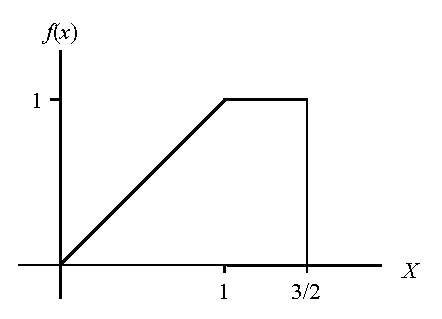
\includegraphics[scale=0.8]{img/vac-3}
\end{center}
calcular:

\begin{enumerate}
\item $P(X<1)$, $P(X>0)$, $P(X=1/4)$, $P(1/2\leq X\leq 3/2)$.
\item Media y desviación típica.
\end{enumerate}
}
%SOLUCIÓN
{}
%RESOLUCIÓN
{}


\newproblem{vac-4}{amb}{*}
%ENUNCIADO
{Se sabe que la duración de las baterías de un tipo de marcapasos (expresada en años) es una variable aleatoria cuya
función de densidad es
\[
f(x)=
\begin{cases}
0 & \text{si $x<0$,}\\
\dfrac{e^{-x/10}}{10} & \text{si $x\geq 0$.}
\end{cases}
\]
Se pide:
\begin{enumerate}
\item Comprobar que $f(x)$ es función de densidad.
\item Calcular la función de distribución.
\item Calcular la probabilidad de que la batería dure menos de 5 años, y de que dure entre 5 y 10 años.
\item Calcular la vida media de la batería.
\end{enumerate}
}
%SOLUCIÓN
{
\begin{enumerate}
\item $\int_{-\infty}^\infty f(x)\, dx = [-e^{-x/10}]_{-\infty}^\infty = 1$.
\item \[
F(x)=
\begin{cases}
0 & \text{si $s<0$,}\\
1-e^{-x/10} & \text{si $x\geq 0$.}
\end{cases}
\]
\item $P(X<5)=0.3935$ y $P(5<X<10)=0.2387$.
\item $\mu=10$ años.
\end{enumerate}
}
%RESOLUCIÓN
{}


\newproblem*{vac-5}{amb}{*}
% ENUNCIADO
{La proporción de cierto aditivo en la gasolina determina su precio. Si en la producción de gasolina la proporción de
aditivo es una variable aleatoria $X$ con función de densidad $f(x)=6x(1-x)$ para $0\leq x\leq 1$, de manera que si
$x<0,5$ la gasolina es del tipo I y se vende a $0.6$ \euro/l, si $0.5\leq x\leq 0.8$ la gasolina es del tipo II y se
vende a $0.7$ \euro/l, y si $x>0.8$ la gasolina es del tipo III que se vende a $0.8$ \euro/l, se pide:
\begin{enumerate}
\item Calcular la función de distribución de $X$.
\item Calcular los porcentajes de producción de cada tipo de gasolina.
\item Calcular el precio medio por litro.
\end{enumerate}
}
%SOLUCIÓN
{}
%RESOLUCIÓN
{}


\newproblem{vac-6}{gen}{}
%ENUNCIADO
{Un empleado suele acudir al trabajo en cualquier instante entre las 6 y las 7 con igual probabilidad. Se pide:
\begin{enumerate}
\item Calcular la función de densidad de la variable que mide el instante en que acude a trabajar y dibujarla.
\item Calcular la función de distribución y dibujarla.
\item Calcular la probabilidad de que llegue entre las 6 y cuarto y las 6 y media.
\item Calcular la hora media a la que se espera que llegue.
\end{enumerate}
}
%SOLUCIÓN
{
\begin{enumerate}
\item \[
f(x)=
\begin{cases}
0 & \text{si $x<6$,}\\
1 & \text{si $6\leq x\leq 7$,}\\
0 & \text{si $7<x$.}
\end{cases}
\]
\item \[
F(x)=
\begin{cases}
0 & \text{si $x<6$,}\\
x-6 & \text{si $6\leq x\leq 7$,}\\
1 & \text{si $7<x$.}
\end{cases}
\]
\item $P(6.25<X<6.5)=0.25$.
\item $\mu=6.5$, es decir, a las 6 horas y media.
\end{enumerate}
}
%RESOLUCIÓN
{}


\newproblem{vac-7}{gen}{}
%ENUNCIADO
{Sea $Z$ una variable aleatoria que sigue una distribución $N(0,1)$.
Determinar el valor de $t$ en cada uno de los siguientes casos: 
\begin{enumerate}
\item El área entre $0$ y $t$ es $0.4783$.
\item El área a la izquierda de $t$ es $0.6406$.
\item El área entre $-1.5$ y $t$ es $0.2313$.
\end{enumerate}
}
%SOLUCIÓN
{
\begin{enumerate}
\item $t=2.02$.
\item $t=0.36$.
\item $t=-0.53$.
\end{enumerate}
}
%RESOLUCIÓN
{}


\newproblem*{vac-8}{gen}{}
%ENUNCIADO
{Hallar las siguientes probabilidades:

\begin{enumerate}
\item  $P(-2.4$ $\leq Z\leq -1.2)$ si $Z$ es $N(0,1)$.
\item  $P(\left| Z\right| >1.2)$ si $Z$ es $N(0,1)$.
\item  $P(1.3\leq X\leq 3.3)$ si $X$ es $N(2,1)$.
\item  $P(\left| X-3\right| >2)$ si $X$es $N(3,4)$.
\end{enumerate}
}
%SOLUCIÓN
{}
%RESOLUCIÓN
{}


\newproblem*{vac-9}{gen}{*}
%ENUNCIADO
{Supongamos una variable aleatoria $X$ que sigue una distribución normal de desviación típica 1 ($\sigma =1)$, y media ($\mu )$ desconocida. Si nos dan como dato que la función de densidad en $x$=1 vale $\dfrac{1}{\sqrt{2\pi }},$ y teniendo en cuenta que la función de densidad viene dada por:
\[
f(x)=\dfrac{1}{\sigma \sqrt{2\pi }}\ e^{-\dfrac{(x-\mu )^{2}}{2\sigma ^{2}}},
\]
calcular $P(\left| X-2\right| <3)$.
}
%SOLUCIÓN
{}
%RESOLUCIÓN
{}


\newproblem{vac-10}{med}{}
%ENUNCIADO
{Se sabe que el nivel de colesterol en varones de más de 30 años sigue una distribución normal, de media 220 mg/dl y desviación típica 30 mg/dl. Realizando un estudio sobre 20000 varones mayores de 30 años,
\begin{enumerate}
\item ¿Cuántos se espera que tengan su nivel de colesterol entre 210 y 240 mg/dl?
\item Si un nivel de colesterol por encima de 250 mg/dl puede provocar trombosis, ¿cuántos tienen riesgo de trombosis?
\item ¿Cuál será el nivel de colesterol por encima del cual está el 20\% de la población?
\end{enumerate}
}
%SOLUCIÓN
{
\begin{enumerate}
\item $P(210\leq X\leq 240)=0.3781\rightarrow 7561.3$  varones. 
\item $P(X>250)=0.1587\rightarrow 3173.1$ varones. 
\item $P_{80}=245.2486$ mg/dl. 
\end{enumerate}
}
%RESOLUCIÓN
{}


\newproblem{vac-11}{med}{}
%ENUNCIADO
{Entre los diabéticos, el nivel de glucosa en la sangre en ayunas, puede suponerse de distribución aproximadamente
normal, con media 106 mg/100 ml y desviación típica 8 mg/100 ml.
\begin{enumerate}
\item Calcular la probabilidad de que una persona diabética elegida al azar tenga un nivel de glucosa inferior a  120mg/100ml.
\item ¿Qué porcentaje de diabéticos tendrá niveles entre 90 y 120 mg/100 ml?
\item Calcular e interpretar el primer cuartil del nivel de glucosa. 
\end{enumerate}
}
%SOLUCIÓN
{
\begin{enumerate}
\item $P(X\leq 120)=0.9599$.
\item $P(90< X<120)=0.9371$, es decir, un $93.71\%$.
\item $100.64$ mg/$100$ ml. 
\end{enumerate}
}
%RESOLUCIÓN
{}


\newproblem*{vac-12}{gen}{}
%ENUNCIADO
{Se sabe que la distribución de probabilidad de una variable aleatoria $X$ sigue la ley normal. Si conocemos $P(X>3.6)=0.3821$ y $P(X<5.8)=0.9192$, calcular $\mu $ y $\sigma $ de la distribución normal.
}
%SOLUCIÓN
{}
%RESOLUCIÓN
{}


\newproblem{vac-13}{med}{}
%ENUNCIADO
{En una población con 40000 personas, se sabe que 2276 tienen entre 0.80 y 0.84 miligramos de bilirrubina por decilitro
de sangre, y que 11508 tienen más de 0.84.
Suponiendo que la concentración de bilirrubina en sangre sigue una distribución normal, se pide:  
\begin{enumerate}
\item Calcular su media y su desviación típica.
\item Calcular el número de personas con más de 1 miligramo de bilirrubina por decilitro de sangre.
\end{enumerate}
}
%SOLUCIÓN
{
\begin{enumerate}
\item $\mu=0.7$ mg y $\sigma=0.25$ mg.
\item $P(X>1)=0.1151$ y el número de personas con más de 1 mg de bilirrubina es $0.1151\cdot 40000=4604$.
\end{enumerate}
}
%RESOLUCIÓN
{}


\newproblem{vac-14}{gen}{*}
%ENUNCIADO
{En un examen, el 63\% de los alumnos ha obtenido una nota superior a 5, y el 44\% entre 5 y 7.
Suponiendo que las notas siguen una distribución normal:

\begin{enumerate}
\item  Calcular la media y la desviación típica de las notas.
\item  Calcular el porcentaje de alumnos con nota superior a 8.
\item  ¿Cuál es la nota por encima de la cual está el 5\% de los alumnos?
\end{enumerate}
}
%SOLUCIÓN
{Llamando $X$ a la nota obtenida en el examen, se tiene que $X\sim N(\mu,\sigma)$.
\begin{enumerate}
\item $\mu=5.55$ puntos y $\sigma=1.65$ puntos.
\item $P(X>8)=0.0648$, es decir, el $6.48\%$ de los alumnos han tenido una nota superior a 8.
\item $8.21$ puntos.
\end{enumerate}
}
%RESOLUCIÓN
{}


\newproblem*{vac-15}{med}{*}
%ENUNCIADO
{Se realiza un estudio sobre la tensión arterial máxima en varones de edad comprendida entre 30 y 40 años. Como
consecuencia del estudio se sabe que el 40\% la tiene por encima de 140 mmHg y el 20\% por debajo de 110 mmHg.
Suponiendo que la tensión arterial máxima sigue una distribución normal, se pide:
\begin{enumerate}
\item Calcular la media y la desviación típica.
\item Calcular el porcentaje de hipertensos, si se considera hipertenso a una persona cuya tensión arterial máxima sea mayor que 150 mmHg.
\item ¿Cuál es el valor de la tensión arterial máxima por encima del cual se espera que esté el 10\% de la población?
\end{enumerate}
}
%SOLUCIÓN
{}
%RESOLUCIÓN
{}


\newproblem{vac-16}{gen}{*}
%ENUNCIADO
{Un grupo de 100 alumnos realiza un examen. Una vez corregido, el profesor observa que la nota media es $4.2$ y que 32 alumnos han tenido una calificación superior a $5$. Suponiendo que las notas siguen una distribución normal, ¿cuántos alumnos habrán obtenido una calificación superior a $7$?
}
%SOLUCIÓN
{$P(X>7)=0.0508\rightarrow 5.1$ alumnos.
}
%RESOLUCIÓN
{}


\newproblem{vac-17}{med}{*}
%ENUNCIADO
{Se supone que la tensión arterial de los habitantes de una población de 20000 habitantes sigue una distribución
normal, cuya media es 13 y su rango intercuartílico 4.
Se pide:
\begin{enumerate}
\item ¿Cuántas personas tienen una tensión por encima de 16?
\item ¿Cuánto tendrá que disminuir la tensión de una persona que tiene 16 para situarse en el 40\% de la población con
tensión más baja?
\end{enumerate}
}
%SOLUCIÓN
{
\begin{enumerate}
\item $P(X>16)=0.1587$ y el número de personas con tensión por encima de 16 mmHg es $0.1587\cdot 20000=3174$.
\item Debe disminuir $3.75$ mmHg.
\end{enumerate}
}
%RESOLUCIÓN
{}


\newproblem{vac-18}{med}{*}
%ENUNCIADO
{En una población de 30000 individuos se está interesado en medir el volumen sanguíneo de sus individuos.
Se sabe que la desviación típica de la población es $0.4$ litros y que el 50\% de los individuos tienen un volumen
superior a $4.8$ litros.
¿Cuántos individuos presentarán un volumen menor de $4.3$ litros?}
%SOLUCIÓN
{El número de individuos con menos de $4.3$ litros de sangre es $3168$.}
%RESOLUCIÓN
{}


\newproblem*{vac-19}{med}{}
%ENUNCIADO
{Se sabe que el nivel de potasio en personas sanas sigue una distribución normal de media $4.4$ mg/l y desviación típica $0.4$ mg/l. En un estudio realizado sobre 20000 personas sanas:

\begin{enumerate}
\item  ¿Cuántos se espera que tengan un nivel de potasio entre $3.7$ y $5$ mg/l?
\item  ¿Cuántos se espera que tengan un nivel de potasio por encima de $5.3$ mg/l?
\item  ¿Cuál será el nivel de potasio por encima del cual está la cuarta parte de la población?
\end{enumerate}
}
%SOLUCIÓN
{}
%RESOLUCIÓN
{}


\newproblem{vac-20}{gen}{}
% ENUNCIADO
{Se consideran las variables aleatorias $X_1$ y $X_2$. La variable $X_1$ sigue una distribución normal de media $\mu$ y
desviación típica $\sigma$, mientras que la variable $X_2$ sigue también una distribución normal de media $\mu + 1$ y
desviación típica $\sigma$. Si la probabilidad de que $X_1$ tome valores superiores a $14.2$ es $0.5636$, y la de que
$X_2$ tome valores inferiores a $17.4$ es $0.6103$, se pide:
\begin{enumerate}
\item Hallar los valores de $\mu$ y $\sigma$.
\item Si se rechazan los individuos que están fuera del intervalo $(12,18)$, hallar los porcentajes de rechazo
correspondientes a $X_1$ y $X_2$.
\item Si se desea seleccionar el $20\%$ de individuos que tengan los valores más altos de $X_1$, ¿cuál será el valor
de $X_1$ a partir del cuál se seleccionarán?
\end{enumerate}
}
%SOLUCIÓN
{
\begin{enumerate}
\item $\mu=15$ y $\sigma=5$.
\item $P(12<X_1<18)=0.4515$, luego el porcentaje de rechazos es $100\%-45.15\%=54.85\%$.\\
$P(12<X_2<18)=0.4436$, luego el porcentaje de rechazos es $100\%-44.36\% = 55.64\%$.
\item $19.21$.
\end{enumerate}
}
%RESOLUCIÓN
{}


\newproblem{vac-21}{med}{*}
% ENUNCIADO
{El peso de los recién nacidos no prematuros en una ciudad sigue una distribución normal de media y desviación típica
desconocidas.
Teniendo en cuenta que, de un total de 200 recién nacidos no prematuros, 15 han pesado más de 4 kg y 25 menos de $2,5$
kg:
\begin{enumerate}
\item ¿Cuáles son la media y la desviación típica del peso?
\item ¿Cuántos niños no prematuros habrán nacido con un peso entre $3$ y $3.5$ kg?
\item Si los médicos consideran peligrosos los pesos por debajo del percentil 10, ¿cuál será dicho peso?, ¿cuántos
niños habrán nacido con un peso por debajo de dicho percentil?
\end{enumerate}
}
%SOLUCIÓN
{Llamando $X$ al peso de los recién nacidos no prematuros, se tiene que $X\sim N(\mu,\sigma)$.
\begin{enumerate}
\item $\mu=3.17$ kg y $\sigma=0.58$ kg.
\item 66 niños.
\item $P_{10}=2.43$ kg y habrán nacido 20 niños por debajo de este peso.
\end{enumerate}
}
%RESOLUCIÓN
{}


\newproblem*{vac-22}{amb}{}
%ENUNCIADO
{La cantidad de fuel en aguas costeras próximas al hundimiento de un petrolero sigue una distribución normal de media 20 $\mu$g/l y desviación típica 8 $\mu$g/l. Si se considera que existe contaminación si el nivel de fuel excede los 5 $\mu$g/l, ¿Cual es la probabilidad de que al realizar una medición al azar no se detecte la contaminación? ¿Y si en lugar de realizar una medición, realizamos dos y tomamos la media?
}
%SOLUCIÓN
{}
%RESOLUCIÓN
{}


\newproblem*{vac-23}{med}{*}
%ENUNCIADO
{Una solución contiene virus bacteriófagos $T_4$ en una concentración de $4\cdot10^6$ por mm$^3$.
En la misma solución hay $2\cdot10^6$ bacterias por mm$^3$.
Suponiendo que todos los virus infectan bacterias y que se distribuyen al azar entre las mismas, se pide:
\begin{enumerate}
\item ¿Cuál es el porcentaje de bacterias que no están infectadas por el virus?
\item ¿Qué porcentaje de bacterias tendrá al menos 2 virus fijados sobre ellas?
\item Si tomamos un volumen pequeño de dicha solución en el que hay 4 bacterias, ¿cuál es la probabilidad de que alguna
esté infectada?
\item Si tomamos un volumen en el que hay 10000 bacterias, ¿cuál es la probabilidad de que estén infectadas al menos 8600?
\end{enumerate}
}
%SOLUCIÓN
{}
%RESOLUCIÓN
{}


\newproblem{vac-24}{psi}{}
%ENUNCIADO
{El coeficiente intelectual es una puntuación derivada de los test de inteligencia que tiene media 100 puntos y
desviación típica 15.
Si se considera que una persona por encima de 145 es una superdotada, ¿qué porcentaje de superdotados habrá en la
población?
Si se considera que el 1\% de las personas con menor coeficiente intelectual son deficientes, ¿por debajo de qué
coeficiente estarán dichas personas? }
%SOLUCIÓN
{Llamando $X$ al coeficiente intelectual, se tiene que $X\sim N(100,15)$.\\
$P(X>145)=0.0013$, luego el $0.13\%$ de las personas son superdotadas.\\
$P_1=65.10$, por debajo de este coeficiente las personas son deficientes.}
%RESOLUCIÓN
{}


\newproblem*{vac-25}{amb}{*}
%ENUNCIADO
{Si se supone que la concentración de plomo en suelo sigue una distribución normal de media 320 mg/Kg y desviación típica desconocida, y sabiendo que el 25\% de los suelos presenta una concentración de plomo por abajo de 240 mg/Kg:
\begin{enumerate}
\item ¿Cuánto vale la desviación típica de la distribución?
\item Suponiendo que niveles de Plomo por arriba de 250 mg/Kg son peligrosos para la salud, y se catalogan como contaminados todos los suelos que sobrepasen ese nivel, ¿cuál es la probabilidad de que un suelo analizado esté contaminado?
\item Si analizamos 10000 suelos diferentes, ¿cuántos esperamos que no estén contaminados?
\item ¿Cuánto vale el rango intercuartílico de la distribución? ¿Qué interpretación tienen?
\end{enumerate}
}
%SOLUCIÓN
{}
%RESOLUCIÓN
{}


\newproblem*{vac-26}{amb}{*}
%ENUNCIADO
{Para la recuperación de una lesión en encinas parasitadas por un tipo de hongo se dispone de dos tratamientos alternativos A y B. El tiempo de recuperación con el procedimiento A sigue una distribución normal de media 16 meses y desviación típica 3 meses, mientras que con el procedimiento B la media es de 20 meses y la desviación típica de 1.
\begin{enumerate}
\item ¿Qué tanto por ciento de recuperaciones se producen con cada tratamiento entre 18 y 21 meses?
\item ¿Qué tratamiento consigue antes la recuperación del 90\% de las encinas tratadas?. Justificar adecuadamente la respuesta.
\item Si a una encina le aplicamos los dos tratamientos, que suponemos que actúan de forma independiente, ¿cuál es la
probabilidad de que cure antes de 19 meses?
\end{enumerate}
}
%SOLUCIÓN
{}
%RESOLUCIÓN
{}


\newproblem*{vac-27}{gen}{}
%ENUNCIADO
{Calcular:
\begin{enumerate}
\item  $P(T\leq 1.476)$ si $T\sim T(5)$.
\item  $P(T\geq 0.69)$ si $T\sim T(16)$.
\item  El valor $t_{0}$ tal que $P(T<t_{0})=0.995$, con $T\sim T(12)$.
\item  El valor $t_{0}$ tal que $P(T>t_{0})=0.01$, con $T\sim T(8)$.
\end{enumerate}
}
%SOLUCIÓN
{}
%RESOLUCIÓN
{}


\newproblem*{vac-28}{gen}{}
%ENUNCIADO
{Calcular:

\begin{enumerate}
\item  $P(X\leq 5.23)$ si $X\sim \chi ^{2}(12)$.
\item  $P(X\geq 1.65)$ si $X\sim \chi ^{2}(8)$.
\item  El valor $x_{0}$ tal que $P(X<x_{0})=0.995$, con $X\sim \chi ^{2}(18)$.
\item  El valor $x_{0}$ tal que $P(X>x_{0})=0.25$, con $X\sim \chi ^{2}(7)$.
\end{enumerate}
}
%SOLUCIÓN
{}
%RESOLUCIÓN
{}


\newproblem*{vac-29}{gen}{}
%ENUNCIADO
{Calcular:

\begin{enumerate}
\item  El valor $f_{0}$ tal que $P(F<f_{0})=0.9$, con $F\sim F(12,8)$.
\item  El valor $f_{0}$ tal que $P(F>f_{0})=0.025$, con $F\sim F(5,7)$.
\end{enumerate}
}
%SOLUCIÓN
{}
%RESOLUCIÓN
{}


\newproblem*{vac-30}{med}{*}
%ENUNCIADO
{Suponiendo que la duración del embarazo sigue una distribución normal de media y desviación típica desconocidas, y
teniendo en cuenta que el 80\% de las mujeres dan a luz antes de 40 semanas, y que el 70\% lo hacen después de 38
semanas y 2 días, se pide:  

\begin{enumerate}
\item Calcular la media y la desviación típica de la distribución dadas en número de semanas.\\
\item Suponiendo un hospital en el que se han producido 2000 nacimientos, ¿cuántos lo habrán hecho con más de 282 días de gestación?
\item Suponiendo una mujer que ha tenido 2 embarazos y que la duración del segundo ha sido independiente del primero, ¿cuál es la probabilidad de que alguno de los partos se haya producido antes de los 275 días de embarazo?
\end{enumerate}
}
%SOLUCIÓN
{}
%RESOLUCIÓN
{}


\newproblem{vac-31}{far}{*}
%ENUNCIADO
{El gasto mensual en medicamentos de las familias españolas antes de la crisis seguía una distribución normal $X\sim
N(160,\sigma)$, mientras que ahora sigue una distribución normal $Y\sim N(\mu,2\sigma)$.
Sabiendo que antes de la crisis el $10\%$ de las familias gastaba más de 200 euros y que después el $40\%$ gastaba
menos de 100 euros, se pide:
\begin{enumerate}
\item ¿Qué porcentaje de familias gastarán ahora entre 110 y 120 euros?
\item ¿Qué percentil de la distribución actual se corresponde con el tercer decil de la distribución de antes de la crisis?
\end{enumerate}
}
%SOLUCIÓN
{$X\sim N(160,\,31.25)$ y $Y\sim N(115.625,\,62.50)$.
\begin{enumerate}
\item $P(110\leq Y\leq 120)=0.0638$.
\item El decil tercero en $X$ es $D_3=143.75$ euros y se corresponde aproximadamente con el percentil 67 de $Y$. 
\end{enumerate}
}
%RESOLUCIÓN
{\begin{enumerate}
\item Teniendo en cuenta que el gasto antes de la crisis seguía una distribución normal de media 160 euros y desviación típica desconocida, pero nos dan el dato de que antes de la crisis el $10\%$ de las familias gastaba más de 200, fácilmente podemos aprovechar este dato para calcular la desviación típica, y utilizamos esta desviación típica y el dato de que el $40\%$ de las familias gastan ahora menos de 100 euros para calcular la media del gasto después. Con ello, podemos calcular la probabilidad que nos piden: $P(110 \leq Y \leq 120)$.
Utilizamos el dato de que $P(X>200)=0.1000$:
\begin{align*}
P(X > 200) &= 1 - P(X \le 200) = 1 - P\left( {Z \le \frac{{200 - 160}}{\sigma }} \right) = 1 - P\left( {Z \le \frac{{40}}{\sigma }} \right) =\\
&= 1 - F\left( {\frac{{40}}{\sigma }} \right)=0.1000 \Leftrightarrow F\left( {\frac{{40}}{\sigma }} \right) = 0.9000.
\end{align*}

Mediante la tabla de la distribución normal tipificada vemos que $F(1.28)=0.8997$, que es la probabilidad acumulada más cercana al $0.9000$ que buscamos. Por lo tanto:
\[
\frac{{40}}{\sigma } = 1.28 \Leftrightarrow \sigma  = \frac{{40}}{{1.28}} = 31.25\;\mbox{euros}.
\]

Para calcular la media $\mu$ del gasto después, utilizamos el dato de que $P(Y<100)=0.4000$:
\begin{align*}
P(Y < 100) &= P\left({Z \le \frac{{100 - \mu }}{{2\sigma }}} \right) = P\left( {Z \le \frac{{100 - \mu }}{{2 \cdot 31.25}}} \right) = P\left( {Z \le \frac{{100 - \mu }}{{62.50}}} \right)=\\
&=F\left( {\frac{{100 - \mu }}{{62.50}}} \right)=0.4000.
\end{align*}
De nuevo, buscamos en la tabla de la normal tipificada y observamos que $F(-0.25)=0.4013$, que es la probabilidad acumulada más cercana al $0.4000$ que buscamos. Por lo tanto:
\[
\frac{{100 - \mu }}{{62.50}} =  - 0.25 \Leftrightarrow \mu  = 100 + 15.625 = 115.625\,\mbox{euros}.
\]

Por lo tanto, concluimos que $X\sim N(160\,,\,31.25)$ y $Y\sim N(115.625\,,\,62.50)$.

Por último, calculamos la probabilidad (el porcentaje) de que el gasto ahora esté entre 110 y 120 euros:
\begin{align*}
P(110 \le Y \le 120) &= P\left( {\frac{{110 - 115.625}}{{62.50}} \le Z \le \frac{{120 - 115.625}}{{62.50}}} \right) = P\left( { - 0.09 \le Z \le 0.07} \right) =\\
&= F(0.07) - F( - 0.09) \stackrel{1}{=} 0.5279 - 0.4641 = 0.0638=6.38\%.
\end{align*}
\begin{quotation}
\footnotesize (1) Mirando en la tabla de la función de distribución de la normal estándar.
\end{quotation}

\item Para calcular el tercer decil de antes de la crisis, sabemos que $P(X\leq D_3)=0.3000$. Por lo tanto:
\[
P\left( {Z \le \frac{{D_3  - 160}}{{31.25}}} \right) = F\left( {\frac{{D_3  - 160}}{{31.25}}} \right) = 0.3000
\]
Mediante la tabla de la normal tipificada, la probabilidad acumulada más cercana es: $F(-0.52)=0.3015$. Por lo tanto:
\[
\frac{{D_3  - 160}}{{31.25}} =  - 0.52 \Leftrightarrow D_3  = 143.75\,\mbox{euros},
\]
y para ver qué porcentaje de familias consumen ahora, durante la crisis, menos de $143.75$ euros:
\[
P(Y \le 143.75) = P\left( {Z \le \frac{{143.75 - 115.625}}{{62.50}}} \right) = P(Z \le 0.45) = F(0.45) = 0.6736.
\]
Por lo tanto, los $143.75$ euros son el percentil 67 de la distribución de gasto durante la crisis.
\end{enumerate}
}


\newproblem{vac-32}{psi}{}
%ENUNCIADO
{Un test diagnóstico para niños de 10 años con problemas de lectura da puntuaciones que se distribuyen normalmente con
una media de 80 y una varianza de 100.
Se pide:
\begin{enumerate}
\item Dar la probabilidad de que un niño seleccionado al azar tenga una puntuación de:
\begin{enumerate}
\item menos de 68;
\item entre 75 y 90;
\end{enumerate} 
\item El test indica que el niño tiene un problema del lenguaje si su puntuación está por debajo del 10\% de la
población que realizó el test.
¿Por debajo de qué puntuación el test diagnosticará problemas de lenguaje?
\item Si se selecciona una muestra de 16 niños:
\begin{enumerate}
\item ¿Cuantos se espera que tengan una puntuación por encima de 68?
\item ¿Cuál es la probabilidad de que su puntuación media supere los 84 puntos?
\end{enumerate}
\end{enumerate}
}
%SOLUCIÓN
{Llamando $X$ a la puntuación del test diagnóstico, se tiene que $X\sim N(80,10)$.
\begin{enumerate}
\item $P(X<68)=0.1151$ y $P(75<X<90)=0.5328$.
\item $P_{10}=67.18$ puntos.
\item $P(X>68)=0.8849$ y el número esperado niños con puntuaciones por encima de 68 es \mbox{$0.8849\cdot 16=14.16$}.\\
$\bar x\sim N(80,\,2.5)$ y $P(\bar x>84)=0.0548$.
\end{enumerate}
}
%RESOLUCIÓN
{}


\newproblem{vac-33}{fis}{*}
%ENUNCIADO
{El tiempo de recuperación de una determinada lesión de rodilla en futbolistas profesionales sigue una distribución normal de media 50 días
y desviación típica 10 días. Si dentro de 65 días hay una final, ¿cuál es la probabilidad de que un jugador profesional que acaba de
lesionarse la rodilla se pierda la final? Si las semifinales son dentro de 40 días y se acaban de lesionar la rodilla 4 jugadores, ¿cuál es
la probabilidad de que alguno de ellos pueda jugar la semifinal?
}
%SOLUCIÓN
{Llando $X$ a la variable aleatoria que mide el número de días que tarda en recuperarse un futbolista con la lesión de rodilla, 
$P(X>65)=0.0668$.\\
Llamando $Y$ a la variable aleatoria que mida el número de jugadores que tardan menos de 40 días en curarse de entre los 4 que tenemos
lesionados, $P(Y\geq 1)=0.499$.
}
%RESOLUCIÓN
{Llamemos $X$ a la variable aleatoria que mide el número de días que tarda en recuperarse un futbolista con la lesión de rodilla. Entonces,
según el enunciado, $X\sim N(50,10)$. La probabilidad de que un futbolista tarde más de 65 días en curarse es $P(X>65)$. Para calcularla, tipificamos
\[
P(X>65)=P(\frac{X-50}{10}>\frac{65-50}{10})=P(Z>1.5)=1-P(Z\leq 1.5)=1-F(1.5),
\]
y mirando en la tabla de la función de distribución de la normal estándar, la probabilidad acumulada hasta 1.5 es 0.9332. Por tanto,
$P(X>65)=1-0.9332=0.0668.$

Para responder a la segunda pregunta, necesitamos otra variable aleatoria que mida el número de jugadores que tardan menos de 40 días en
curarse de entre 4 que tenemos lesionados. Llamemos $Y$ a dicha variable. Puesto que $Y$ responde a un esquema de repetición de pruebas (una
por jugador), donde cada prueba consiste en ver si el jugador tarda menos de 40 días en curarse (éxito) o no (fracaso), entonces sigue una
distribución binomial de parámetros $n=4$ jugadores y $p=P(X<40)$.

Necesitamos, en primer lugar, calcular esta probabilidad. Al igual que antes, tipificando y mirando en la tabla de la función de
distribución de la normal estándar obtenemos
\[
P(X<40)=P(\frac{X-50}{10}<\frac{40-50}{10})=P(Z<-1)=F(-1)=0.1587.
\]
Así pues, $Y\sim B(4,0.1587)$, y la probabilidad que nos piden es
\[
P(Y\geq 1)=1-P(Y<1)=1-P(Y=0)=1-\binom{4}{0}0.1587^0 (1-0.1587)^4=1-0.8413^4=0.499.
\]
}


\newproblem{vac-34}{fis}{*}
%ENUNCIADO
{Según el teorema central del límite, se sabe que para muestras grandes ($n\geq 30$) la media muestral $\bar x$ sigue una distribución
normal $N(\mu,\sigma/\sqrt{n})$, donde $\mu$ es la media de la población y $\sigma$ su desviación típica.

Se sabe que en una población la elongación del triceps sural tiene una media de 60 cm y una desviación típica de 15 cm. Si se toma una
muestra de tamaño 30, ¿cuál es la probabilidad de obtener una media muestral mayor de 62? Si se considera que una muestra es atípica si su
media muestral está por debajo del percentil 5 de su distribución, ¿se puede considerar atípica una muestra de 60 individuos con
$\bar x=57$?}
%SOLUCIÓN
{
\begin{enumerate}
\item Llamando $\bar X$ a la variable que mide la elongación media del triceps sural en muestras de tamaño 30, $P(\bar X>62)=0.2327$.
\item Llamando $\bar Y$ a la variable que mide la elongación media del triceps sural en muestras de tamaño 60, $P_5=56.8$ cm, luego la
muestra no es atípica.
\end{enumerate}
}
%RESOLUCIÓN
{Sea $\bar X$ la variable que mide la elongación media del triceps sural en muestras de tamaño 30. Por el teorema central del límite,
puesto que tomamos una muestra grande, tenemos que $\bar X\sim N(\mu,\sigma/\sqrt{n})=N(60,15/\sqrt{30})=N(60\,,\,2.74)$. Así pues, la
probabilidad que nos piden es
\begin{align*}
P(\bar X>62)& \stackrel{(1)}{=} P\left(\frac{\bar X-60}{2.74}>\frac{62-60}{2.74}\right)= P(Z>0.73) =\\
&= 1 - P(Z\leq 0.73)=1-F(0.73)\stackrel{(2)}{=}1-0.7673=0.2327.
\end{align*}
\begin{quote}
    \footnotesize
    (1) Tipificando.\\
    (2) Mirando en la tabla de la función de distribución de la normal estándar.
\end{quote}

Para responder a la segunda pregunta, llamemos $\bar Y$ a la variable que mide la elongación media del triceps sural en muestras de tamaño
60. Al igual que antes, por el teorema central del límite, $N(\mu,\sigma/\sqrt{n})=N(60,15/\sqrt{60})=N(60\,,\,1.94)$. Para saber si una
muestra es atípica, tenemos que calcular el percentil 5 de $\bar Y$.
Dicho valor cumplirá $P(\bar Y\leq y_0)=0.05$. Tipificando tenemos
\[
P(\bar Y\leq y_0)=
P\left(\frac{\bar Y-60}{1.94}\leq\frac{y_0-60}{1.94}\right)=
P\left(Z\leq\frac{y_0-60}{1.94}\right)=F\left(\frac{y_0-60}{1.94}\right)=0.05.
\]
Y buscando en la tabla de la función de distribución de la normal estándar, tenemos que
\[
\frac{y_0-60}{1.94}=-1.65 \Leftrightarrow y_0=-1.65\cdot 1.94+60= 56.8 \text{ cm}.
\]
Como la media muestral obtenida es 57 y no está por debajo de $56.8$ que es el percentil 5, concluimos que la muestra obtenida no se puede
considerar atípica. 
}


\newproblem{vac-35}{far}{*}
%ENUNCIADO
{Para el tratamiento de una enfermedad se utilizan 3 fármacos diferentes: $A$ en un 20\% de los casos, $B$ en un 30\%, y $C$ en un 50\%. Los
tratados con $A$ curan en media al cabo de $6.2$ días con una desviación típica de $1.1$ días; los tratados con $B$ en $7.1$ días con una
desviación típica de $1.3$ y los tratados con $C$ en $7.4$ días con una desviación típica de $0.9$. Con ello:
\begin{enumerate}
\item En qué fármaco es mayor el percentil $90$, en $B$ o en $C$?
\item Qué probabilidad total hay de que tomado un enfermo al azar haya curado antes de $8.1$ días?
\item Sabiendo que un enfermo ha tardado en curar más de $7.2$ días, con qué fármaco es más probable que haya sido tratado? Justificar
adecuadamente la respuesta.
\end{enumerate}
}
%SOLUCIÓN
{Llamando $X$ al tiempo de curación y $A$, $B$ y $C$ a los sucesos consistentes en haber sido tratado respectivamente con cada uno de los
fármacos:
\begin{enumerate}
\item El percentil 90 en el fármaco $B$ es $8.7660$ días y en $C$ es $8.5534$ días, así que es mayor en el fármaco $B$.
\item $P(X<8.1)=0.8161$.
\item $P(A/X>7.2)=0.0771$, $P(B/X>7.2)=0.2989$ y $P(C/X>7.2)=0.624$, así que es más probable que haya sido tratado con el fármaco $C$.
\end{enumerate}
}
%RESOLUCIÓN
{}


\newproblem{vac-36}{far}{*}
%ENUNCIADO
{Se sabe que la concentración de urea láctica, en mg/cm$^3$, en vacas sanas sigue una distribución normal de media $28$ y desviación típica
$1.5$, mientras que en vacas con una determinada enfermedad sigue una distribución normal de media $34.5$ y desviación típica $2$. Para
detectar la enfermedad se realiza un test diagnóstico que da positivo cuando el nivel de urea láctica está por encima de $32$. Se pide:
\begin{enumerate}
\item ¿Qué sensibilidad $P(+/E)$ y qué especificidad $P(-/\overline{E})$ tiene el test diagnóstico?
\item Si el test da positivo en un 5\% de los casos analizados, ¿cuál será el porcentaje de vacas enfermas en la población?
\item Teniendo en cuenta el porcentaje de vacas enfermas anterior, ¿cuál será la probabilidad de diagnóstico acertado con este test?
\end{enumerate}
}
%SOLUCIÓN
{\begin{enumerate}
\item $P(+/E)=0.8944$ y $P(-/\overline E)=0.9962$.
\item $P(E)=0.0465$.
\item $P(E\cap +)+P(\overline E\cap -)= 0.0416 + 0.9498 = 0.99143$.
\end{enumerate}
}
%RESOLUCIÓN
{}


\newproblem{vac-37}{gen}{*}
%ENUNCIADO
{Sea $Z$ una variable aleatoria continua que sigue un modelo de distribución normal estándar $N(0,1)$.
Calcular las siguientes probabilidades utilizando la tabla de la función de distribución.
\begin{enumerate}
\item $P(Z<1.24)$
\item $P(Z>-0.68)$
\item $P(-1.35\leq Z\leq 0.44)$
\end{enumerate}
}
%SOLUCIÓN
{
\begin{enumerate}
\item $P(Z<1.24)=0.8925$.
\item $P(Z>-0.68)=0.7517$.
\item $P(-1.35\leq Z\leq 0.44)=0.5815$.
\end{enumerate}
}
%RESOLUCIÓN
{}


\newproblem{vac-38}{gen}{*}
%ENUNCIADO
{Sea $Z$ una variable aleatoria continua con distribución normal estándar.
Determinar el valor de $x$ en los siguientes casos utilizando la tabla de la función de distribución.
\begin{enumerate}
\item $P(Z<x)=0.6406$.
\item $P(Z>x)=0.0606$.
\item $P(0\leq Z\leq x)=0.4783$.
\item $P(-1.5\leq Z\leq x)=0.2313$.
\item $P(-x\leq Z\leq x)=0.5467$.
\end{enumerate}
}
%SOLUCIÓN
{
\begin{enumerate}
\item $x=0.3601$. 
\item $x=1.5498$. 
\item $x=2.0198$.
\item $x=−0.5299$. 
\item $x=0.7499$.
\end{enumerate}
}
%RESOLUCIÓN
{}


\newproblem{vac-39}{gen}{*}
%ENUNCIADO
{Sea $X$ una variable aleatoria continua con distribución normal $N(10,2)$.
\begin{enumerate}
\item Calcular $P(X\leq 10)$.
\item Calcular $P(8\leq X\leq 14)$.
\item Calcular el rango intercuartílico. 
\item Calcular el tercer decil. 
\end{enumerate}
}
%SOLUCIÓN
{
\begin{enumerate}
\item $P(X\leq 10)=0.5$.
\item $P(8\leq X\leq 14)=0.8186$. 
\item $RI=2.698$.
\item $D_3=8.9512$.
\end{enumerate}
}
%RESOLUCIÓN
{
}


\newproblem{vac-40}{nut}{*}
%ENUNCIADO
{Un estudio trata de determinar el efecto de una dieta baja en grasas sobre el tiempo de vida de un tipo de ratas. 
Las ratas se dividieron en dos grupos, uno con una dieta normal y el otro con una dieta baja en grasas. 
Se supone que el tiempo de vida sigue un modelo de distribución normal con igual varianza pero con distintas medias. 
Si el 20\% de las ratas con dieta normal vivieron más de 12 meses, el 5\% vivieron menos de 8 meses y el 85\% de las ratas con dieta baja en grasas vivieron más de 11 meses, 
\begin{enumerate}
\item ¿Cuál es la media y la desviación típica del tiempo de vida de las ratas con una dieta baja en grasas?
\item Si en el experimento había un 40\% de ratas con dieta normal y un 60\% de ratas con dieta baja en grasas, ¿cuál es la probabilidad de que una rata elegida al azar muera antes de 9 meses?
\end{enumerate}
}
%SOLUCIÓN
{Llamando $X$ al tiempo de vida de las ratas. 
\begin{enumerate}
\item $\mu=12.6673$ meses y $s=1.6087$ meses. 
\item $P(X<9)=0.068$.
\end{enumerate}
}
%RESOLUCIÓN
{}


\newproblem{vac-41}{med}{*}
%ENUNCIADO
{Un test diagnóstico para detectar el dopaje en atletas da un resultado positivo cuando la concentración de una determinada sustancia en sangre es mayor de 4 $\mu$g/ml.
Si la distribución de la concentración de a sustancia en sangre en atletas dopados sigue un modelo de distribución normal con media $4.5$
$\mu$g/ml y desviación típica $0.2$ $\mu$g/ml, y en atletas no dopados sigue un modelo de distribución normal con media $3$ $\mu$g/ml y desviación típica $0.3$ $\mu$g/ml, 
\begin{enumerate}
\item ¿cuál es la sensibilidad y la especificidad del test?
\item Si hay un $10\%$ de atelas dopados en una competición, ¿cuál es el valor predictivo positivo del test? 
\end{enumerate}
}
%SOLUCIÓN
{Llamando $D$ al suceso aleatorio consistente en estar dopado, $X$ a la concentración de la sustancia en atletas dopados e $Y$ a la concentración de la sustancia en atletas no dopados.
\begin{enumerate}
\item Sensibilidad $P(+|D)=P(X>4)=0.9938$ y especificidad $P(-|\bar D)=P(Y<4)=0.9996$.
\item VPP $P(D|+)=0.9961$.
\end{enumerate}
}
%RESOLUCIÓN
{}
% Author Alfredo S�nchez Alberca (asalber@ceu.es)

\newproblem{ico-1}{gen}{}
% ENUNCIADO
{Una muestra aleatoria de tamaño $81$ extraída de una población normal con $\sigma ^2=64$, tiene una $\overline{x}=78$.
Calcular el intervalo de confianza del $95\%$ para $\mu$.
}
%SOLUCIÓN
{$\mu\in 79\pm 1.742 = (76.258,\,79.742)$.
}
%RESOLUCIÓN
{}


\newproblem{ico-2}{nut}{}
% ENUNCIADO
{Para determinar si un pescado es o no apto para el consumo por su contenido en Hg (mercurio), se realizan $15$
valoraciones obteniendo una media de $0.44$ ppm (partes por millón) de Hg, y una desviación típica de $0.08$ ppm.
Calcular los límites de confianza para la media, a un nivel de significación $\alpha =0.1.$ }
% SOLUCIÓN
{
$\mu\in 0.44\pm 0.0376$ ppm = $(0.4024\text{ppm},\,0.4776\text{ppm})$.
}
% RESOLUCIÓN
{}


\newproblem{ico-3}{qui}{}
% ENUNCIADO
{Se obtuvieron cinco determinaciones del pH de una solución con los siguientes resultados: 
\[7.90\quad 7.85\quad 7.89\quad 7.86\quad 7.87.\]
Hallar unos límites de confianza de la media de todas las determinaciones del pH de la misma solución, al nivel de
significación $\alpha =0.01.$
}
% SOLUCIÓN
{
$\mu \in 7.874\pm 0.0426 = (7.8314,\,7.9166)$.
}
% RESOLUCIÓN
{}


\newproblem{ico-4}{med}{}
% ENUNCIADO
{Se desea saber cuál debe ser el tamaño muestral mínimo de una muestra para poder realizar la estimación de la tasa media
de glucosa plasmática de una determinada población, con un nivel de confianza $0.95$ y pretendiendo una amplitud de $2.5$
mg.

\noindent NOTA: En una muestra previa de tamaño 10 se obtuvo una desviación típica de 10 mg.
}
%SOLUCIÓN
{
249 individuos.
}
%RESOLUCIÓN
{}


\newproblem{ico-5}{far}{}
%ENUNCIADO
{Para que un fármaco sea efectivo, la concentración de un determinado principio activo debe ser 20 mg/mm$^3$.
Se recibe un lote de dicho fármaco y se analizan 10 para medir la concentración del principio activo, obteniendo los
resultados siguientes:
\[
17.6 \quad 19.2 \quad 21.3 \quad 15.1 \quad 17.6 \quad 18.9 \quad 16.2 \quad 18.3 \quad 19 \quad 16.4.
\]
En vista de los resultados, ¿podremos rechazar el lote con una confianza $0.95$ de no equivocarnos?
}
%SOLUCIÓN
{
$17.96\pm 1.278$ mg/mm$^3$ = $(16.682\text{mg/mm}^3,\,19.238\text{mg/mm}^3)$.
}
%RESOLUCIÓN
{}


\newproblem*{ico-6}{nut}{*}
%ENUNCIADO
{En un estudio sobre el consumo anual de litros de cerveza entre la población de menores de 18 años de una ciudad se
obtuvo la siguiente muestra: 
\[ 42\quad 16\quad 60\quad 29\quad 7\quad 20\quad 30\quad 25\quad 38\quad 5.\]
Se pide:
\begin{enumerate}
\item Calcular el intervalo de confianza del 95\% para la media. Si se considera que un consumo medio por encima de 40
litros es peligroso, ¿existen pruebas significativas para afirmar que la población de partida no está en peligro?
\item ¿Qué tamaño muestral mínimo hubiese sido necesario para conseguir un intervalo de confianza de amplitud 5?
\end{enumerate}
}
%SOLUCIÓN
{}
%RESOLUCIÓN
{}


\newproblem*{ico-7}{amb}{}
%ENUNCIADO
{En una explotación minera se mide el contenido en mercurio de las rocas extraídas.
Tras analizar 20 rocas, se obtiene un contenido medio del $10.8\%$ y una desviación típica de $2.7\%$. Se pide: 
\begin{enumerate}
\item Si, para que la explotación sea rentable, el porcentaje medio de contenido de mercurio debe ser superior al
10\%, ¿existen pruebas para afirmar que la explotación será rentable?
\item ¿Y si para que la explotación sea rentable, el contenido de mineral debe tener cierta uniformidad ($\sigma<3$)?
\end{enumerate}
}
%SOLUCIÓN
{}
%RESOLUCIÓN
{}


\newproblem*{ico-8}{amb}{}
%ENUNCIADO
{Para ver si una población de aves se ha visto afectada por los vertidos tóxicos de una fábrica, se pretende estimar
la proporción de aves contaminadas con metales pesados.
Para ello se realiza un sondeo preliminar con 30 aves, de las que 5 resultan estar contaminadas.
Se pide:
\begin{enumerate}
\item Construir un intervalo de confianza del 95\% para la proporción de aves contaminadas.
\item Si se desea estimar la proporción con un error máximo de $\pm 2\%$, ¿qué tamaño muestral habría que tomar?
\end{enumerate}
}
%SOLUCIÓN
{}
%RESOLUCIÓN
{}


\newproblem{ico-9}{far}{}
%ENUNCIADO
{Se realizó un estudio sobre el contenido de principio activo de un determinado fármaco a partir de una muestra,
determinándose los siguientes resultados en mg/cm$^{3}$:
\[ 46.4-46.1-45.8-47.0-46.1-45.9-45.8-46.9-45.2-46.0. \]
Obtener un intervalo de confianza del 95\% para la varianza del contenido de principio activo de dicho fármaco,
suponiendo que sigue una distribución normal.
}
%SOLUCIÓN
{
$\sigma^2 \in (0.1356(\text{mg/cm}^3)^2,\,0.9541(\text{mg/cm}^3)^2)$.
}
%RESOLUCIÓN
{}


\newproblem{ico-10}{med}{}
%ENUNCIADO
{Se desea hacer un estudio estadístico sobre el número de hematíes en las mujeres.
Se selecciona una muestra de 25 mujeres y se obtiene un número medio de hematíes de 4300000 con una desviación típica
de 200000 (en cada milímetro cúbico de sangre).
Calcular el intervalo de confianza para la media y la varianza del número de hematíes de las mujeres en la población,
con un nivel de significación $0.1$.
}
%SOLUCIÓN
{
Intervalo de confianza del 95\% para la media: $\mu \in 4.3\cdot 10^6\pm 69850$ hematíes = $(4230150,\,4369850)$.\\
Intervalo de confianza del 95\% para la varianza: $\sigma^2\in (2747\cdot 10^10,\,7246\cdot 10^10)$ hematíes$^2$. 
}
%RESOLUCIÓN
{}


\newproblem*{ico-11}{med}{*}
%ENUNCIADO
{Para determinar el nivel medio de colesterol en la sangre de una población, se realizaron análisis sobre una muestra
de 8 personas, obteniéndose los siguientes resultados:
\begin{center}
196 -- 212 -- 188 -- 206 -- 203 -- 210 -- 201 -- 198
\end{center}
Hallar intervalos de confianza para la media y la varianza de nivel de colesterol con un nivel de significación 0.1, suponiendo que el nivel de colesterol en la población sigue una distribución normal.
}
%SOLUCIÓN
{}
%RESOLUCIÓN
{}


\newproblem{ico-12}{med}{}
%ENUNCIADO
{Para determinar la concentración media de albúmina en la sangre se realizaron mediciones sobre un grupo experimental
obteniéndose los siguientes resultados, expresados en g/l: 
\[38-42-46-37-49-42-40-36.\]
Obtener un intervalo de confianza para la varianza de la población con un nivel de significación $0.05$.
}
%SOLUCIÓN
{
$\sigma^2\in (8.844\text{g}^2/\text{l}^2,\,83.728\text{g}^2/\text{l}^2)$.
}
%RESOLUCIÓN
{}


\newproblem{ico-13}{med}{}
%ENUNCIADO
{El tiempo que tarda en hacer efecto un analgésico sigue una distribución aproximadamente normal.
En una muestra de 20 pacientes se obtuvo una media de $25.4$ minutos y una desviación típica de $5.8$ minutos.
Calcular el intervalo de confianza del 90\% e interpretarlo.
¿Cuántos pacientes habría que tomar para poder estimar la media con una precisión de $\pm 1$ minuto? }
%SOLUCIÓN
{Intervalo de confianza del 90\% para $\mu$: $(23.0992,\,27.7008)$.\\
Tamaño muestral para una precisión de $\pm 1$ minuto: $n=96$.}
%RESOLUCIÓN
{}


\newproblem{ico-14}{med}{}
%ENUNCIADO
{En un estudio para el estado de la salud oral de una ciudad, se tomó una muestra elegida al azar de 280 varones entre
35 y 44 años y se contó el número de piezas dentarias en la boca.
Tras la revisión pertinente, los dentistas informaron que había 70 individuos con 28 o más dientes.
Se desea realizar una estimación por intervalo de confianza de la proporción de individuos de esta ciudad con 28
dientes o más, con un nivel de confianza $0.95$.
}
%SOLUCIÓN
{
$p\in 0.25\pm 0.0507 = (0.1993,\,0.3007)$.
}
%RESOLUCIÓN
{}


\newproblem*{ico-15}{med}{}
%ENUNCIADO
{Leemos en una revista médica que la cuarta parte de los cancerosos de cierto tumor de estómago presentan vómitos, con
una precisión o tolerancia del 10\% y con una confianza del 99\%.
¿Con cuántos pacientes se ha realizado el estudio?
}
%SOLUCIÓN
{}
%RESOLUCIÓN
{}


\newproblem{ico-16}{med}{*}
%ENUNCIADO
{Un país está siendo afectado por una epidemia de un virus.
Para valorar la gravedad de la situación se tomaron 40 personas al azar y se comprobó que 12 de ellas tenían el virus.
Determinar el intervalo de confianza para el porcentaje de infectados con un nivel de significación $0.05$.
}
%SOLUCIÓN
{
$p\in (0.1580,\,0.4420)$ con un 95\% de confianza.
}
%RESOLUCIÓN
{}


\newproblem{ico-17}{gen}{}
%ENUNCIADO
{Se desea obtener un intervalo de confianza del 95\% para la diferencia de marcas obtenidas por chicos y chicas en una
prueba física.
Se toma una muestra de 50 chicas y 75 chicos, obteniendo las chicas una marca media de 76 y los chicos de 82.
Además, se conocen las desviaciones típicas de las marcas obtenidas en las poblaciones de chicas y chicos, que son 6 y
8 respectivamente.
}
%SOLUCIÓN
{
$\mu_1-\mu_2 \in 6\pm 2.458$ puntos = $(3.542\text{puntos},\,8.458)$.
}
%RESOLUCIÓN
{}


\newproblem*{ico-18}{amb}{}
%ENUNCIADO
{Las temperaturas medias mensuales (en $^\circ$C) durante el año 2001 en Madrid y Sevilla fueron:
\begin{center}
\begin{tabular}{|l|r|r|r|r|r|r|r|r|r|r|r|r|}
\hline
Ciudad &    Ene &    Feb &    Mar &    Abr &    May &    Jun &    Jul &    Ago &    Sep &    Oct &    Nov &    Dic \\
\hline
 Madrid                  &  $7.2$ &  $8.4$ & $12.2$ & $13.7$ & $16.7$ & $23.3$ & $24.2$ & $25.5$ & $20.4$ & $16.2$ &  $8.1$ &  $4.2$ \\
\hline
 Sevilla                 & $12.1$ & $13.6$ & $16.8$ & $19.0$ & $20.9$ & $27.0$ & $26.6$ & $28.2$ & $24.7$ & $21.3$ & $13.8$ & $11.5$ \\
\hline
\end{tabular}
\end{center}
¿Existen diferencias significativas en las temperaturas medias de ambas ciudades?
}
%SOLUCIÓN
{}
%RESOLUCIÓN
{}


\newproblem{ico-19}{fis}{}
%ENUNCIADO
{Se está ensayando un nuevo procedimiento de rehabilitación para una cierta lesión.
Para ello se trataron nueve pacientes con el procedimiento tradicional y otros nueve con el nuevo, y se midieron los
días que tardaron en recuperase, obteniéndose los siguientes resultados:
\begin{center}
\begin{tabular}{ll}
Método tradicional: & 32\quad 37\quad 35\quad 28\quad 41\quad 44\quad 35\quad 31\quad 34\\
Método nuevo: & 35\quad 31\quad 29\quad 25\quad 34\quad 40\quad 27\quad 32\quad 31
\end{tabular}
\end{center}
Se desea obtener un intervalo de confianza del 95\% para la diferencia de las medias del tiempo de recuperación
obtenido con ambos procedimientos.
Se supone que los tiempos de recuperación siguen una distribución normal, y que las varianzas son aproximadamente
iguales para los dos procedimientos.
}
%SOLUCIÓN
{
$\mu_1-\mu_2\in 3.667\pm 4.712$ días = $(-1.045\text{ días},\,8.379\text{ días})$.
}
%RESOLUCIÓN
{}


\newproblem{ico-20}{med}{}
%ENUNCIADO
{En un hospital pediátrico se comprobó que de 200 niños con un determinado síndrome, 48 murieron antes de cumplir un
año de edad, mientras que sólo 25 de 125 niñas con el mismo síndrome murieron.
¿Se puede afirmar con cierta seguridad que el síndrome es más letal en los niños que en las niñas?
}
%SOLUCIÓN
{
$p_1-p_2 \in 0.04\pm 0.077 = (-0.037,\,0.117)$ luego no se puede afirmar que el síndrome sea más letal en los niños que
en las niñas con un 95\% de confianza.}
%RESOLUCIÓN
{}


\newproblem{ico-21}{med}{}
%ENUNCIADO
{Se ha realizado un estudio para investigar el efecto del ejercicio físico en el nivel de colesterol en la sangre. En el estudio
participaron once personas, a las que se les midió el nivel de colesterol antes y después de desarrollar un programa de ejercicios. Los
resultados obtenidos fueron los siguientes
\begin{center}
\begin{tabular}{ccc}
\toprule 
Persona & Nivel previo & Nivel posterior \\ 
1 & 182 & 198 \\
2 & 232 & 210 \\ 
3 & 191 & 194 \\ 
4 & 200 & 220 \\ 
5 & 148 & 138 \\ 
6 & 249 & 220 \\ 
7 & 276 & 219 \\ 
8 & 213 & 161 \\
9 & 241 & 210 \\ 
10 & 280 & 213 \\ 
11 & 262 & 226 \\ 
\bottomrule
\end{tabular}
\end{center}
Hallar un intervalo de confianza del 90\% para la diferencia del nivel medio de colesterol antes y después del ejercicio.
}
%SOLUCIÓN
{
$\mu_{x_1-x_2}\in 24.0909\pm 19.4766$ mg/dl = $(4.6143\text{mg\dl},\, 43.5675\text{mg/dl})$.
}
%RESOLUCIÓN
{}


\newproblem{ico-22}{qui}{}
%ENUNCIADO
{Dos químicos $A$ y $B$ realizan 14 y 16 determinaciones, respectivamente, de plutonio.
Los resultados obtenidos se muestran en la siguiente tabla
\begin{center}
\begin{tabular}{cc|cc}
\multicolumn{2}{c|}{$A$} & \multicolumn{2}{c}{$B$} \\ \hline
263.36 & 254.68 & 286.53 & 254.54 \\
248.64 & 276.32 & 284.55 & 286.30 \\
243.64 & 256.42 & 272.52 & 282.90 \\
272.68 & 261.10 & 283.85 & 253.75 \\
287.33 & 268.41 & 252.01 & 245.26 \\
287.26 & 282.65 & 275.08 & 266.08 \\
250.97 & 284.27 & 267.53 & 252.05 \\
&  & 253.82 & 269.81
\end{tabular}
\end{center}
Se pide:

\begin{enumerate}
\item Calcular intervalos de confianza del 95\% de confianza para cada caso.
\item ¿Se puede decir que existen diferencias significativas en la media?
\end{enumerate}
}
%SOLUCIÓN
{
\begin{enumerate}
\item Intervalo de confianza del 95\% para la media de $A$: $\mu_A \in 266.98\pm 8.681 = (258.299,\,275.661)$.\\
Intervalo de confianza del 95\% para la media de $B$: $\mu_B \in 267.91\pm 7.677 = (260.233,\,275.587)$.
\item $\mu_A-\mu_B \in -0.93\pm 11.020 = (-11.95,\,10.92)$, luego no hay diferencias significativas en las medias con
un 95\% de confianza.
\end{enumerate}
}
%RESOLUCIÓN
{}


\newproblem{ico-23}{med}{*}
%ENUNCIADO
{Un equipo de investigación está interesado en ver si una droga reduce el colesterol en la sangre.
Con tal fin se toma una muestra de 10 pacientes y determina el contenido de colesterol antes y después del tratamiento.
Los resultados expresados en miligramos por cada 100 mililitros son los siguientes:
\[
\begin{tabular}{ccccccccccc}
\toprule
Paciente & 1 & 2 & 3 & 4 & 5 & 6 & 7 & 8 & 9 & 10 \\
Antes & 217 & 252 & 229 & 200 & 209 & 213 & 215 & 260 & 232 & 216 \\ 
Después & 209 & 241 & 230 & 208 & 206 & 211 & 209 & 228 & 224 & 203 \\
\bottomrule
\end{tabular}
\]
Se pide:

\begin{enumerate}
\item Construir la variable Diferencia que recoja la diferencia entre los niveles de colesterol antes y después del
tratamiento, y calcular el intervalo de confianza con $1-\alpha =0.95$ para la media de dicha variable.
\item A la vista del intervalo anterior, ¿hay pruebas significativas de que la droga disminuye el nivel de colesterol
en sangre?
\end{enumerate}
}
%SOLUCIÓN
{
\begin{enumerate}
\item $\mu_{x_1-x_2}\in 7.4\pm 7.572$ mg/100ml = $(-0.172\text{mg/100ml},\,14.972\text{mg/100ml})$.
\item No se puede afirmar que la droga disminuya el colesterol con un 95\% de confianza.
\end{enumerate}
}
%RESOLUCIÓN
{}


\newproblem*{ico-24}{fis}{*}
%ENUNCIADO
{Se está ensayando un nuevo procedimiento de rehabilitación para una cierta lesión.
Se sabe que de 80 deportistas tratados con el procedimiento tradicional, se recuperaron perfectamente 26, mientras que
de los 20 tratados con el nuevo procedimiento se han recuperado 11.
¿Se puede afirmar con una confianza del 95\% que el nuevo procedimiento es mejor que el tradicional?
}
%SOLUCIÓN
{}
%RESOLUCIÓN
{}


\newproblem{ico-25}{amb}{*}
%ENUNCIADO
{En una muestra aleatoria de 200 personas, 114 están a favor de la fluoración de las aguas.
Se pide:
\begin{enumerate}
\item Hallar el intervalo de confianza del 96\% para la fracción de la población que está a favor de la fluoración de
las aguas.
\item ¿Qué tamaño mínimo de muestras habría que tomar para tener una confianza del 96\% de que la proporción muestral
difiere menos de $0.02$ de la proporción real de la población?
\end{enumerate}
}
%SOLUCIÓN
{
\begin{enumerate}
\item $p\in 0.375\pm 0.197 = (0.178,\,0.572)$.
\item 2634 individuos.
\end{enumerate}
}
%RESOLUCIÓN
{}


\newproblem*{ico-26}{far}{*}
%ENUNCIADO
{Para ver si una campaña de publicidad sobre un fármaco ha influido en sus ventas, se tomó una muestra de 8 farmacias
y se midió el número de fármacos vendidos durante un mes, antes y después de la campaña, obteniéndose los siguientes
resultados:
\begin{center}
\begin{tabular}{ccccccccc}
\toprule
Antes & 147 & 163 & 121 & 205 & 132 & 190 & 176 & 147  \\
Después & 150 & 171 & 132 & 208 & 141 & 184 & 182 & 145  \\
\bottomrule
\end{tabular}
\end{center}
Obtener la variable diferencia y construir un intervalo de confianza para la media de la diferencia con un nivel de
significación $0.05$.
¿Existen pruebas suficientes para afirmar con un 95 \% de confianza que la campaña de publicidad ha aumentado las
ventas?
}
%SOLUCIÓN
{}
%RESOLUCIÓN
{}


\newproblem{ico-27}{med}{*}
%ENUNCIADO
{Para comparar la eficacia de dos tratamientos $A$ y $B$ en la prevención de repeticiones de infarto de miocardio, se
aplicó el tratamiento $A$ a 80 pacientes y el $B$ a 60.
Al cabo de dos años se observó que habían sufrido un nuevo infarto 14 pacientes de los sometidos al tratamiento $A$ y
15 de los del $B$.
Se pide:
\begin{enumerate}
\item Construir un intervalo de confianza del $95\%$ para la diferencia entre las proporciones de personas sometidas a los tratamientos $A$ y $B$ que no vuelven a sufrir un infarto.
\item A la vista del resultado obtenido, razonar si con ese nivel de confianza puede afirmarse que uno de los tratamientos es más eficaz que el otro.
\end{enumerate}
}
%SOLUCIÓN
{
\begin{itemize}
\item $p_A-p_B\in (-0.2126,\,0.0626)$ con un nivel de confianza del 95\%.
\item No puede afirmarse que un tratamiento sea más eficaz que otro pues la diferencia de medias podría ser positiva,
negativa o cero. 
\end{itemize}
}
%RESOLUCIÓN
{}


\newproblem*{ico-28}{amb}{}
%ENUNCIADO
{La siguiente tabla muestra el porcentaje de industrias españolas y europeas según el consumo de energía primaria de
las mismas durante el año 2002 (se estudiaron 1000 industrias).
\[
\begin{tabular}{|l|c|c|}
\hline
Fuente energética  &  España  & Resto de Europa \\
\hline
Petróleo            & $52.2$\% &    $40.4$\%     \\
Carbón              & $15.2$\% &    $14.8$\%     \\
Nuclear             & $13.0$\% &    $15.2$\%     \\
Gas                 & $12.8$\% &    $23.5$\%     \\
Energías Renovables & $6.5$\%  &     $6.1$\%     \\
Saldo Energético    & $0.2$\%  &       0\%       \\
\hline
\end{tabular}
\]
Estudiar para qué energías el porcentaje de industrias de España es significativamente diferente del resto de Europa.
}
%SOLUCIÓN
{}
%RESOLUCIÓN
{}


\newproblem{ico-29}{nut}{*}
%ENUNCIADO
{En un análisis de obesidad dependiendo del hábitat en niños menores de 5 años, se obtienen los siguientes resultados:
\begin{center}
\begin{tabular}{|l|c|c|}
\cline{2-3}
\multicolumn{1}{l|}{} & Casos analizados & Casos con sobrepeso \\
\hline
Hábitat rural & 1150 & 480 \\
\hline
Hábitat urbano & 1460 & 660 \\
\hline
\end{tabular}
\end{center}
Se pide:

\begin{enumerate}
\item  Construir un intervalo de confianza, con un nivel de significación $0.01$, para la proporción de niños menores
de 5 años con sobrepeso en el hábitat rural. Igualmente para el hábitat urbano.
\item Construir un intervalo de confianza, con un nivel de confianza del $95\%$, para la diferencia de proporciones de
niños menores de 5 años con sobrepeso entre el hábitat rural y el urbano.
A la vista del resultado obtenido, ¿se puede concluir, con un $95\%$ de confianza, que la proporción de niños menores
de 5 años con sobrepeso depende del hábitat?
\end{enumerate}
}
%SOLUCIÓN
{
\begin{enumerate}
\item $p_R \in (0.3799,\,0.4548)$ y $p_U\in (0.4185,\,0.4856)$ con un 99\% de confianza.
\item $p_R-p_U\in (-0.0729,\,0.0036)$ con un nivel de confianza del 95\%, luego no se puede afirmar que haya
diferencias en las proporciones de niños menores de 5 años con sobrepeso.
\end{enumerate}
}
%RESOLUCIÓN
{}


\newproblem*{ico-30}{med}{}
%ENUNCIADO
{Se ha realizado un estudio con 1000 mujeres que han dado a luz recientemente, elegidas al azar entre los registros de
los diferentes hospitales de la comunidad de Madrid, para saber si un nuevo protocolo (visitas al médico y consumo de
ciertos fármacos) resulta más efectivo para prevenir las infecciones (ya sean pre, intra o postparto).
Del total, 750 han seguido el protocolo habitual, entre las cuales 35 han sufrido algún tipo de infección; mientras
que 250 han seguido el protocolo nuevo y 9 de ellas han padecido alguna infección.
¿Se puede afirmar, con un 95\% de confianza, que la proporción de mujeres que ha tenido algún tipo de infección ha
sido diferente según el protocolo utilizado?
}
%SOLUCIÓN
{}
%RESOLUCIÓN
{}


\newproblem*{ico-31}{amb}{*}
%ENUNCIADO
{La siguiente tabla muestra los datos de emisiones de CO$_2$ y CH$_4$ (en Kg/hab) y el producto interior bruto per
cápita (en miles US\$) de varios países en el último año:
\[
\begin{array}{|l|r|r|r|}
\hline
\mbox{País} & \mbox{CO}_2 & \mbox{CH}_4 & \mbox{PIB}\\
\hline\hline
\mbox{Austria}     & 7.60 & 0.97 & 38.40\\ \hline
\mbox{España}      & 6.73 & 0.81	& 30.12\\ \hline
\mbox{Francia}     & 5.71 & 0.94	& 33.19\\ \hline
\mbox{EEUU}        &19.40 & 1.72	&	45.84\\ \hline
\mbox{Alemania}    & 9.80 & 0.83	& 34.18\\ \hline
\mbox{Canadá}      &15.60 & 3.08	& 38.43\\ \hline
\mbox{Italia}      & 7.29 & 0.58	& 30.44\\ \hline
\mbox{Japón}       &	9.44 & 0.16	& 33.58\\ \hline
\mbox{Australia}   &17.48 & 6.36	& 36.26\\ \hline
\mbox{Reino Unido} & 8.99 & 0.76	& 35.13\\ \hline
\end{array}
\qquad
\begin{array}{|l|r|r|r|}
\hline
\mbox{País} & \mbox{CO}_2 & \mbox{CH}_4 & \mbox{PIB}\\
\hline\hline
\mbox{Bolivia}     & 1.05 & 3.44	& 40.13\\ \hline
\mbox{Niger}       &	0.1	 & 0.12	&	 0.67\\ \hline
\mbox{Senegal}     &	0.35 & 0.76 &  1.69\\ \hline
\mbox{Pakistán}    & 0.65 & 0.59	&  2.59\\ \hline
\mbox{Filipinas}   &	0.83 & 0.46	&  3.38\\ \hline
\mbox{Perú}        & 0.94 & 0.75	&  7.80\\ \hline
\mbox{Túnez}      & 2.17 & 0.48	&  7.47\\ \hline
\mbox{Nepal}       & 0.13 & 0.90	&  1.21\\ \hline
\mbox{Nicaragua}   & 0.7	 & 0.32	&  2.62\\ \hline
\mbox{Mauritania}  & 0.97 & 0.85	&  2.01\\ \hline
\end{array}
\]
¿Existen diferencias significativas en la emisión de CO$_2$ entre los países con un PIB superior a 10 mil US\$ y los
países con un PIB inferior? ¿Y en las emisiones de CH$_4$? Justificar la respuesta.
}
%SOLUCIÓN
{}
%RESOLUCIÓN
{}


\newproblem{ico-32}{gen}{}
%ENUNCIADO
{En una muestra de 250 estudiantes de una universidad, 146 hablaban inglés.
¿Entre qué valores estará el porcentaje de individuos de la universidad que hablan inglés, con un nivel de confianza
del 90\%?
}
%SOLUCIÓN
{
$p\in (0.5327,\,0.6353)$ con un 90\% de confianza.
}
%RESOLUCIÓN
{}


\newproblem{ico-33}{psi}{}
%ENUNCIADO
{Si el porcentaje de indivudos daltónicos de una muestra aleatoria es 18\%, ¿cuál será el mínimo tamaño muestral
necesario para conseguir una estimación del porcentaje de daltónicos con una confianza del 95\% y un error menor del 3\%?
}
%SOLUCIÓN
{
$n=2520$.
}
%RESOLUCIÓN
{}


\newproblem{ico-34}{psi}{}
% ENUNCIADO
{Un psicólogo está estudiando la concentración de una encima en la saliba como un posible indicador de la ansiedad crónica.
En un experimento se tomó una muestra de 12 neuróticos por ansiedad y otra de 10 personas con bajos niveles de ansiedad.
En ambas muestras se midió la concentración de la encima, obteniendo los siguientes resultados:
\[
\begin{array}{rcccccccccccc}
\hline
\mbox{Con ansiedad:} & 2.60 & 2.90 & 2.60 & 2.70 & 3.91 & 3.15 & 3.94 & 2.46 & 2.91 & 3.88 & 3.55 & 3.96\\
\mbox{Sin ansiedad:} & 2.37 & 1.10 & 2.55 & 2.64 & 2.20 & 2.12 & 2.47 & 2.90 & 1.66 & 2.72 \\
\hline
\end{array}
\]
¿Se puede concluir a partir de estos datos que la población de neuróticos con ansiedad y la población de personas sin
ansiedad son diferentes en el nivel medio de concentración de encimas?
Justificar la respuesta.
}
%SOLUCIÓN
{
$\frac{\sigma_1^2}{\sigma_2^2}\in (0.3383,\,4.7486)$ con un nivel de confianza del 95\%, luego se puede suponer que las
varianzas son iguales.\\
$\mu_1-\mu_2\in (0.4296,\,1.4510)$ con un 95\% de confianza, luego se puede concluir que hay diferencias entre las
medias.}
%RESOLUCIÓN
{}


\newproblem{ico-35}{gen}{}
%ENUNCIADO
{Las notas en Estadística de una muestra de 10 alumnos han sido:
\begin{center}
$6.3$, $5.4$, $4.1$, $5.0$, $8.2$, $7.6$, $6.4$, $5.6$, $4.3$, $5.2$
\end{center}
Dar una estimación puntual de la nota media, de la varianza y del porcentaje de aprobados en la clase.
}
%SOLUCIÓN
{$\bar x= 5.81$ puntos, $\hat s^2=1.7721$ puntos$^2$ y $\hat p=0.8$.}
%RESOLUCIÓN
{}


\newproblem{ico-36}{psi}{}
%ENUNCIADO
{Para estudiar si la estación del año influye en el estado de ánimo de la gente, se ha tomado una muestra 12 personas y
se ha medido su nivel de depresión en verano e invierno mediante un cuestionario con puntuaciones de 0 a 100 (a mayor
puntuación mayor depresión). Los resultados obtenidos fueron:
\begin{center}
\begin{tabular}{|l|r|r|r|r|r|r|r|r|r|r|r|r|}
\hline
Invierno & 65 & 72 & 84 & 31 & 80 & 61 & 75 & 52 & 73 & 79 & 85 & 71\\
\hline
Verano &   60 & 51 & 81 & 45 & 62 & 53 & 70 & 52 & 64 & 51 & 67 & 62\\
\hline
\end{tabular}
\end{center}
¿Se puede afirmar que la estación del año influye en el estado de ánimo de la gente con un 99\% de confianza?
¿Cómo influye?
}
%SOLUCIÓN
{
No se puede afirmar que la estación influya en el estado de ánimo ya que la media de la diferencia está en
$(-0.7498,\,19.0831)$ con un 99\% de confianza.}
%RESOLUCIÓN
{}


\newproblem{ico-37}{psi}{}
%ENUNCIADO
{Para realizar una determinada tarea se necesitan personas con un cierto nivel de pericia.
Una empresa está interesada en contratar a un grupo de personas que tengan la pericia necesaria para realizar la tarea,
pero que además sean bastante homogéneas en cuanto a la pericia, es decir, que su rendimiento sea parecido.
Para ver si un grupo de alumnos que se han formado en dicha tarea cumplen los requisitos, se ha tomado una muestra y se
les ha sometido una prueba para ver cuántas tareas son capaces de realizar con éxito en una hora.
Los resultados obtenidos fueron:
\begin{center}
16 - 12 - 14 - 21 - 11 - 15 - 17 - 15 - 18 - 24 - 10 - 14 - 17 - 14 
\end{center}
Se pide: 
\begin{enumerate}
\item Si la empresa busca un grupo de empleados capaces de realizar una media de al menos 12 tareas por hora, ¿se puede
afirmar con una confianza del 95\% que el grupo lo cumple?
\item Si la empresa busca que entre los trabajadores haya una dispersión media de $\sigma<3$ tareas, ¿se puede afirmar
con una confianza del 95\% que el grupo lo cumple? 
\end{enumerate} 
}
%SOLUCIÓN
{
\begin{itemize}
\item Lo cumple ya que $\mu\in (13.4026,\,17.7403)$ con un 95\% de confianza.
\item No lo cumple ya que $\sigma \in (2.7232,\,6,0516)$ con un 95\% de confianza.
\end{itemize}
}
%RESOLUCIÓN
{}


\newproblem*{ico-38}{psi}{}
%ENUNCIADO
{Se cree que el consumo de tabaco va ligado al consumo de alcohol y para corroborar esta hipótesis se ha realizado un
estudio en el que se han obtenido los siguientes datos
\begin{center}
\begin{tabular}{lcc}
 & Bebedores & No bebedores\\
\cline{2-3}
Fumadores & \multicolumn{1}{|c}{487} & \multicolumn{1}{c|}{137} \\
No fumadores & \multicolumn{1}{|c}{312} & \multicolumn{1}{c|}{365}\\
\cline{2-3}
\end{tabular}
\end{center}
¿Se puede afirmar que existe relación entre el consumo de tabaco y el de alcohol?
Justificar la respuesta.
}
%SOLUCIÓN
{}
%RESOLUCIÓN
{}


\newproblem{ico-39}{far}{*}
%ENUNCIADO
{Para analizar la eficacia de un determinado fármaco para aumentar las horas de sueño se realiza un estudio con 8 pacientes a los que se les
controla durante todo un mes, en el que no toman el medicamento y se cuantifica la media de las horas de sueño para cada uno de ellos. El
mismo proceso se lleva a cabo durante todo un mes en el que sí que toman el fármaco. Los resultados (en horas de sueño) aparecen en la
siguiente tabla:
\[
\begin{array}{ccc}
\hline
\text{Paciente} & \text{Sin el fármaco} & \text{Con el fármaco} \\
\hline
    1     &        8.3        &         9.0         \\
    2     &        6.9        &         8.1         \\
    3     &        7.2        &         9.2         \\
    4     &        9.1        &         9.5         \\
    5     &        8.2        &         8.5         \\
    6     &        7.5        &         9.0         \\
    7     &        6.1        &         8.0         \\
    8     &        7.4        &         7.9         \\
\hline
\end{array}
\]
¿Se puede concluir con un nivel de confianza del 99\% que el fármaco ha sido eficaz para aumentar las horas de sueño?
}
%SOLUCIÓN
{El intervalo de confianza de 99\% para la media de la diferencia entre las horas de sueño sin el fármaco y con el fármaco es
$(-1.9067\,,\,-0.2183)$, luego si se puede concluir que el fármaco ha sido eficaz para aumentar las horas de sueño.
}
%RESOLUCIÓN
{Para ver si el fármaco ha sido eficaz necesitamos calcular el intervalo de confianza para la media de la diferencia entre horas de sueño
sin y con el fármaco. Al tratarse de datos pareados, construimos una nueva variable $X$ que recoja esta diferencia.
\[
\begin{array}{cccc}
\hline
\text{Paciente} & \text{Sin el fármaco} & \text{Con el fármaco} & X=\text{Diferencia} \\
\hline 
    1     &        8.3        &         9.0         & -0.7\\
    2     &        6.9        &         8.1         & -1.2\\
    3     &        7.2        &         9.2         & -2.0\\
    4     &        9.1        &         9.5         & -0.4\\
    5     &        8.2        &         8.5         & -0.3\\
    6     &        7.5        &         9.0         & -1.5\\
    7     &        6.1        &         8.0         & -1.9\\
    8     &        7.4        &         7.9         & -0.5\\
\hline
\end{array}
\]

Puesto que tenemos una muestra pequeña (8 pacientes), debemos utilizar el intervalo de confianza de la t de Student, cuya fórmula es
\[
\bar x\pm t(n-1)_{\alpha/2}\frac{\hat s}{\sqrt{n}}.
\]
Calculamos primero los estadísticos necesarios para construir el intervalo
\begin{align*}
\bar x &= \frac{\sum x_{i}}{n}=\frac{-0.7-\cdots -0.5}{8}= \frac{-8.5}{8}=-1.0625,\\
s^2 &= \frac{\sum{x_{i}^2}}{n}-\bar x^2=\frac{(-0.7)^2+\cdots +(-0.5)^2}{8}-(-1.0625)^2= \frac{12.29}{8}-1.1289=0.4073,\\
\hat s^2 &= \frac{n}{n-1}\cdot s^2= \frac{8}{7}\cdot 0.4073 = 0.4655,\\
\hat s &= \sqrt{0.4655}=0.6823.
\end{align*}
Como nos piden una confianza del 99\%, $\alpha=0.01$ y el valor de $t(n-1)_{\alpha/2}=t(7)_{0.005}$ lo buscamos en la tabla de la función de
distribución de la t de Student con 7 grados de libertad. Dicho valor es $t(7)_{0.005}=3.499$.

Sustituyendo estos valores en la fórmula del intervalo de confianza, tenemos
\[
-1.0625\pm 3.499\frac{0.6823}{\sqrt{8}}= -1.0625\pm 0.8442,
\]
con lo que el intervalo de confianza resultante es
$(-1.9067\,,\,-0.2183)$.

Según este intervalo, al 99\% de confianza existen pruebas significativas de que la media de la diferencia de horas es negativa y por tanto
el número de horas de sueño después del fármaco aumenta por término medio. Podemos concluir, con un 99\% de confianza, que el fármaco es
eficaz.
}


\newproblem{ico-40}{med}{*}
% ENUNCIADO
{Se quiere probar si la cirrosis hepática hace variar el índice de colinesterasa en suero. Se eligen 2 muestras aleatorias e independientes,
una primera de 60 individuos normales, con media $1.6$ y desviación típica $0.3$, y la segunda de 50 individuos cirróticos, con media $1.1$
y desviación típica $0.4$. ¿Podemos concluir que existen diferencias significativas, con un 99\% de confianza, entre las medias de la
colinesterasa en individuos normales e individuos cirróticos?
}
% SOLUCIÓN
{
}
% RESOLUCIÓN
{
}


\newproblem{ico-41}{med}{*}
% ENUNCIADO
{Un grupo de investigadores obtuvo datos acerca de las concentraciones de amilasa en el suero de muestras de individuos sanos y de
individuos hospitalizados, con el objetivo de determinar si la concentración media es, o no, diferente en ambas poblaciones. Las
concentraciones, en unidades/ml, en 10 individuos sanos fueron:
\begin{center}
\begin{tabular}{llllllllll}
100 & 103 & 96 & 93 & 91 & 104 & 93 & 99 & 88 & 91 \\
\end{tabular}
\end{center}
Y en 12 individuos enfermos fueron:
\begin{center}
\begin{tabular}{llllllllllll}
118 & 115 & 101 & 104 & 116 & 114 & 112 & 113 & 117 & 123&119&121 \\
\end{tabular}
\end{center}

Suponiendo que la concentración de amilasa en suero sigue una distribución normal, tanto en individuos sanos como hospitalizados, y que las
varianzas son desconocidas pero iguales, se pide:
\begin{enumerate}
\item Calcular el intervalo de confianza para la diferencia de medias con un nivel de confianza del 95\%.
\item ¿A qué conclusión deben llegar los investigadores sobre la igualdad o no de la concentración de amilasa? Justificar la respuesta.
\end{enumerate}
}
% SOLUCIÓN
{
}
% RESOLUCIÓN
{
}


\newproblem{ico-42}{med}{*}
% ENUNCIADO
{En un estudio se pretende contrastar el efecto de una vacuna contra la alergia. Para ello, se dispone de un grupo experimental formado por
200 individuos y otro control formado por 300 individuos.
Teniendo en cuenta que en el grupo experimental sufrieron alergia 20 personas, con una duración media de 20 días y una desviación típica de
6, y en el control la sufrieron 42, con una duración media de 25 días y una desviación típica de 7.
Se pide:
\begin{enumerate}
\item Calcular el intervalo de confianza al 90\% para la diferencia de proporciones de los afectados por la alergia entre los que han sido
vacunados y los que no. ¿Se puede concluir que la vacuna ha disminuido significativamente la proporción de afectados por la alergia? Justificar adecuadamente la respuesta. 
\item Suponiendo varianzas poblacionales iguales y que la duración de la alergia sigue una distribución normal, tanto en el grupo
experimental como en el grupo control, calcular el intervalo de confianza del 95\% para la diferencia entre la duración media de la alergia
en el grupo experimental y en el grupo control. ¿Se puede concluir que la vacuna ha disminuido significativamente la duración de la alergia? Justificar adecuadamente la respuesta.  
\end{enumerate}
}
% SOLUCIÓN
{
}
% RESOLUCIÓN
{
}



\section{Estadística Descriptiva}
\begin{enumerate}[leftmargin=*]
\item \useproblem{des-57}
\item \useproblem{des-3a}
\item \useproblem{des-1a}
\item \useproblem{des-24a}
\item \useproblem{des-2a}
\item \useproblem{des-13a}
\item \useproblem{des-3b}
\item \useproblem{des-56a}
\item \useproblem{des-7}
\item \useproblem{des-23}
\item \useproblem{des-29}
\item \useproblem{des-58}
\item \useproblem{des-59}
\item \useproblem{des-20}
\item \useproblem{des-26}
\item \useproblem{des-60}
\item \useproblem{des-61}
\end{enumerate}

\section{Regresión y Correlación}
\begin{enumerate}[leftmargin=*,resume]
\item \useproblem{reg-45}
\item \useproblem{reg-8a}
\item \useproblem{reg-6}
\item \useproblem{reg-3}
\item \useproblem{reg-39}
\item \useproblem{reg-10}
\item \useproblem{reg-11}
\item \useproblem{reg-32}
\item \useproblem{reg-7}
\item \useproblem{reg-25} 
\item \useproblem{reg-41}
\item \useproblem{reg-24}
\item \useproblem{reg-26}
\item \useproblem{reg-44}
\end{enumerate}

\section{Probabilidad}
\begin{enumerate}[leftmargin=*,resume]
\item \useproblem{pro-33}
\item \useproblem{pro-46}
\item \useproblem{pro-47}
\item \useproblem{pro-48}
\item \useproblem{pro-2}
\item \useproblem{pro-3}
\item \useproblem{pro-5}
\item \useproblem{pro-8}
\item \useproblem{pro-9}
\item \useproblem{pro-13}
\item \useproblem{pro-17}
\item \useproblem{pro-16}
\item \useproblem{pro-51}
\item \useproblem{pro-52}
\item \useproblem{pro-53}
\item \useproblem{pro-49}
\item \useproblem{pro-14}
\item \useproblem{pro-19}
\item \useproblem{pro-44}
\item \useproblem{pro-50}
\item \useproblem{pro-24}
\item \useproblem{pro-41}
\end{enumerate}

\section{Variables Aleatorias Discretas}
\begin{enumerate}[leftmargin=*,resume]
\item \useproblem{vad-1}
\item \useproblem{vad-2}
\item \useproblem{vad-3}
\item \useproblem{vad-5}
\item \useproblem{vad-8}
\item \useproblem{vad-7}
\item \useproblem{vad-10}
\item \useproblem{vad-11}
\item \useproblem{vad-15}
\item \useproblem{vad-19}
\item \useproblem{vad-38}
\item \useproblem{vad-18}
\item \useproblem{vad-28}
\end{enumerate}

\section{Variables Aleatorias Continuas}
\begin{enumerate}[leftmargin=*,resume]
\item \useproblem{vac-3}
\item \useproblem{vac-6}
\item \useproblem{vac-37}
\item \useproblem{vac-38}
\item \useproblem{vac-39}
\item \useproblem{vac-11}
\item \useproblem{vac-10}
\item \useproblem{vac-16}
\item \useproblem{vac-13}
\item \useproblem{vac-17}
\item \useproblem{vac-40}
\item \useproblem{vac-41}
\item \useproblem{vac-34}
\item \useproblem{vac-33}
\end{enumerate}

% \section{Estimación de parámetros}
% \begin{enumerate}[leftmargin=*,resume]
% \item \useproblem{ico-1}
% \item \useproblem{ico-2}
% \item \useproblem{ico-3}
% \item \useproblem{ico-4}
% \item \useproblem{ico-7}
% \item \useproblem{ico-13}
% \item \useproblem{ico-14}
% \item \useproblem{ico-16}
% \item \useproblem{ico-21}
% \item \useproblem{ico-19}
% \item \useproblem{ico-23}
% \item \useproblem{ico-22}
% \item \useproblem{ico-27}
% \item \useproblem{ico-29}
% \end{enumerate}

\vspace{2cm}

\textsc{Nota}: Los problemas marcados con una estrella ($\bigstar$) son problemas de
exámenes de otros años.
\end{document}
